%&program=pdflatex

\documentclass[a4paper,final]{memoir} % for a long document

%texindy -L swedish uul804.idx

\usepackage{uul-styles-804}
\usepackage{wrapfig} 
\usepackage[swedish]{babel}
\usepackage{rotating}
\usepackage{index}
\usepackage{multicol}
\usepackage{rotating}
\usepackage{amssymb}
\usepackage{color}
\usepackage{tweaklist}

\newcommand\xfullname{Upptäck Ubuntu Linux 8.04}
\newcommand\xsubtitle{}
\newcommand\xshortname{uul804}
\newcommand\xurl{http://www.hme.se/}
\newcommand\xubuntuver{8.04}
\newcommand\xpackagecount{28~800} %http://packages.ubuntu.com/hardy/allpackages.en.txt.gz
\newcommand\xinstalloption{Ubuntu 8.04 LTS Desktop Edition -- Supported to 2011}

\setsecnumdepth{subsection}
\maxsecnumdepth{subsection}

\title{\xfullname{}}

\trimLmarks

\author{Tobias Hagberg}

\date{} % Delete this line to display the current date

%\makeindex % create an index to be included at the bottom
%\newindex{default}{idx}{ind}{Sak- och personregister}

%%%%%%%%%%

\footmarkstyle{\textsuperscript{#1}}
\setlength{\footmarkwidth}{\parindent}
\setlength{\footmarksep}{-\parindent}
\setlength{\footparindent}{1em}
%\newcommand{\foottextfont}{\footnotesize}

\widowpenalty=9999
\clubpenalty=9999

\newcommand{\xrcredit}[1]{\hbox to 0pt{\hspace*{.6\baselineskip}\begin{rotate}{90}{\usefont{T1}{phv}{m}{n}\selectfont\tiny #1}\end{rotate}}}
\newcommand\xintropic[1]{{\includegraphics[width=85mm]{#1}\xrcredit{\copyright{} Kim Johansson}}\medskip}
\newcommand\xchapter[2]{\chapter{#2}\begin{center}\xintropic{#1}\end{center}}
\newcommand{\xtitleref}[1]{\textit{\titleref{#1}}}

%\newindex{default}{idx}{ind}{Sak- och personregister}

\makeindex

\begin{document}

\renewcommand{\figurename}{Bild} % mti - måste av någon sjuk anledning defineras här för att inte omdefineras

\frontmatter

\def\tocmark{\markboth{Innehåll}{Innehåll}}
\def\indexmark{\markboth{\indexname}{\indexname}}

%\maketitle

\pagestyle{xempty}
\chapterstyle{lfngnonum}

\begin{center}

\fontfamily{fls}\selectfont

~

\vskip 0pt plus 1.125fill

\noindent\textbf{\thetitle}

\vskip 0pt plus 4fill

\end{center}

\newpage

\vbox{\vskip 1cm}

\newpage

\begin{center}

\fontfamily{fls}\selectfont

~

\vskip 0pt plus 1.125fill

\begin{centering}
\noindent
\includegraphics[width=60mm]{bilder804-all/titel}
\end{centering}

\vskip 1.5\baselineskip

\noindent\secheadstyle{\theauthor}

\vskip 0pt plus 5fill

\noindent
\includegraphics[width=22mm]{bilder804-all/logo_final_bw}

\end{center}

\newpage 

\pagestyle{xempty}

{\small{


~

\vskip 0pt plus 1fill


\noindent Boken är typsatt i \LaTeX{} med den fria typsnittsfamiljen Liberation från RedHat och Ascender Corporation. Omslaget är utformat i Inkscape och innehåller en stiliserad variant av Linuxmaskoten Tux, ritad av Larry Ewing.

\medskip

\noindent Copyright \copyright{} 2007, 2008 Tobias Hagberg. 

\medskip

\noindent Förlaget påminner om att varje form av kopiering eller annat mångfaldigande \\
\noindent av text och bild ur denna bok är förbjuden enligt lagen om upphovsrätt.

\medskip

\noindent Tryckt i EU

\medskip

\noindent Andra tryckningen, 2008

\medskip

\noindent ISBN: 978-91-972705-3-3

}}

\newpage 

\pagestyle{lfng}
\chapterstyle{lfng}

\chapter{Om den här utgåvan}

Kul att du har hittat hit! Boken är skriven för att ge dig som inte har så mycket erfarenhet av Linux, men har använt Windows eller Mac~OS en del, en flygande start i Ubuntu. Boken vill ge dig tillräckligt mycket kunskaper för att att du när du har läst ut den ska kunna utforska Ubuntu, och alla tusentals program som ingår, helt på egen hand.

Detta är den andra reviderade och kraftigt utökade utgåvan av Upptäck Ubuntu Linux. Under det knappa år som har gått sedan den första utgåvan kom ut har utvecklarna av Ubuntu hunnit släppa två nya versioner. Utvecklingen av Ubuntu går med taktfasta sjumilakliv, med en ny version en gång i halvåret. Det som är speciellt med den version som den här boken handlar om, Ubuntu 8.04, är att det är en så kallad LTS-release. LTS står för \textit{Long Term Support}, vilket betyder att den här versionen kommer att ha extra lång livslängd, med support och säkerhetsuppdateringar ända till 2011. Om du har funderat på att pröva Linux är Ubuntu 8.04 därför en särskilt bra val -- dina nyvunna kunskaper kommer att stå sig länge. 

Ett stort tack till alla engagerade läsare som har bidragit med idéer och synpunkter på den första utgåvan av boken, bland dem Ingemar Nederman, Lennart Aspenryd, Leif Sandvik, Per-Gunnar Eriksson, Gunne Steen, Martin Adolfsson och Mikael Tillenius. Ett särskilt varm tack till Kim Johansson för de charmigt fyndiga vinjettbilderna med Linuxmaskoten Tux med kompisar \textit{in action}, som inleder varje kapitel.

\vspace*{2\baselineskip}

\noindent Tobias Hagberg


\chapter{Förord}\label{cha:forord}

När jag inte skriver arbetar jag som grafisk formgivare i ett eget företag. Liksom andra grafiska formgivare har jag varit helt beroende av dyra grafik- och layoutprogram som Illustrator, Photoshop och Quark Xpress. Den största enskilda utgiftsposten utöver löpande kostnader som kontorshyra och månadslön har varit programvarulicenser. Men så, för några år sedan, bestämde jag mig för ett experiment. Istället för att använda min gamla kära men allt skraltigare Mac skulle jag köpa en billig bärbar dator och installera Linux på den. Anledningen var att jag hade fått nys om och testat ett trevligt fritt ritprogram som heter Sodipodi. Det var visserligen långt ifrån Illustrator i fråga om funktioner och finesser, men det var kaxigt och kompetent nog för att jag skulle kunna göra det jag behövde -- snabba skisser av idéer såväl som leveransklara illustrationer till kunder. Att använda programmet var till en början ovant och en del krångligare än det smidiga, polerade, Illustrator, men slutresultatet blev lika snyggt som någonsin i Adobe-programmet. Ännu bättre blev det när några av Sodipodi-utvecklarna bestämde sig för att bygga vidare på programmet och göra det mer användarvänligt. Resultatet blev Inkscape\index{Inkscape}, och från första versionen av Inkscape var jag helt såld. För mig får Illustrator-binären på Macens hårddisk numera vila i frid. Inkscape matchar alla mina behov.

Efter ett tag upptäckte jag också ett layoutprogram som heter Scribus\index{Scribus}. Även detta kändes på den tiden lite ruffigt, men utvecklarna hade djärva planer: helt fri, professionell DTP (\textit{desktop publishing}) för Linux, Windows och Mac OS~X. Scribus hade redan tidigt grymt bra stöd för kluriga proffsfunktioner som ICC-färgprofiler, CMYK-färgläge och export av tryck\-opti\-me\-ra\-de PDF-filer. Även här gick det att åstadkomma underverk med lite tålamod. När jag jobbade med programmet råkade jag   på en del buggar. Till en början ryckte jag på axlarna och hittade en väg runt problemet, precis som jag hade lärt mig under alla åren med de kommersiella programmen. Men gradvis började jag inse fördelarna med fri programvara -- som användare har man stora möjligheter att påverka. Jag testade att rapportera ett problem direkt till utvecklarna, och bara efter ett par dagar var buggen fixad. Snabbt blev också Scribus en del av min vardag.

Sedan dess har det gått ruskigt fort. Slag i slag släpps nya versioner av programmen jag använder. Jag är typen som gillar att uppdatera ofta, och nästan varje gång får jag ny inspiration och hittar nya nyttiga funktioner. De är numera lika kapabla och enkla som motsvarande Mac- och Windowsvarianter. Tillsammans med andra fri-programvaru-hittar som Firefox (solklar favorit bland webbläsarna), OpenOffice.org (för att kunna läsa och skriva Microsoft Office-kompatibla dokument), Rhythmbox (för att synka mitt musikbibliotek med min iPod), GIMP och F-spot (för digital bildbehandling och -katalogisering) har jag allt jag behöver, helt gratis. I distributionen Ubuntu Linux finns över \xpackagecount{} program och installationspaket att välja mellan. Jag kunde inte vara mer nöjd. Jag startar ibland min Mac eller öppnar en virtuell Windows-maskin direkt i Linux när jag behöver något kommersiellt, slutet program, men numera händer det väldigt sällan.

Om du är nyfiken på att själv testa Scribus och Inkscape rekommenderar jag dig att först läsa allt fram till och med \Cref{cha:programinstallation}, där du får lära dig hur du på ett busenkelt sätt kan leta efter och installera fler program på din dator.

Slutligen: det går undan i Linuxvärlden. Till exempel uppdaterar olika mjukvaruprojekt och -företag sina program ofta, med betydligt kortare mellanrum än i andra operativsystem. Det har att göra med att utvecklingen av Linuxkärnan, operativsystemet i övrigt och alla de program som körs på det sker i separata, självständiga projekt. Vissa drivs av företag som Novell, RedHat, Sun, Apple och IBM, andra i regi av frivilliga entusiaster. 

För att de olika delarna ska kunna dra nytta av alla andras framsteg så fort som möjligt släpps olika typer av uppdateringar (nya funktioner och buggfixar) kontinuerligt i små paket. Därför uppdateras också ofta de hemsidor som jag rekommenderar i boken, och ibland använder mig av i instruktionerna. Det gör hemsidan för den här boken till en viktig del av läsupplevelsen. Där läggs kontinuerligt upp information och tips om nyheter som gör din tid framför din nyinstallerade Ubuntudator ännu roligare. Adressen till hemsidan är \url{\xurl\xshortname}.

Välkommen in i Linuxland. Jag hoppas du kommer att känna dig lika hemma som jag gör.

\newpage

\settocdepth{subsubsection}

\tableofcontents* % the asterisk means that the contents itself isn't put into the ToC

\mainmatter

\xchapter{bilder804-all/Varfor_Linux}{Varför Linux?}\label{cha:hej}

\index{Linux!varför använda|(}

\xintro{Ubuntu är en mycket populär variant av Linux, ett helt fritt alternativ till Microsoft Windows och andra operativsystem. Ubuntu Linux är ovanligt lättanvänt, ovanligt snyggt och med ett ovanligt bra urval av program.}

I det senare avseendet slår Linux alla konkurrenter med hästlängder. En uppsjö program -- fler än \xpackagecount{}\footnote{http://packages.ubuntu.com/hardy/allpackages.en.txt.gz}  -- finns tillgängliga i Ubuntu med några musklick, helt gratis. Vad du än vill åstadkomma finns det ett fritt program som låter dig göra det. Allt fler upptäcker dessutom mer grundläggande skäl att använda Linux istället för Microsoft Windows eller Mac OS~X -- med Linux har du som användare en mycket större grad av olika friheter. Här går jag igenom några skäl att använda Linux i allmänhet och Ubuntu i synnerhet.

Att använda Linux är ibland ett aktivt val att inte använda Windows, av närmast religiösa skäl för vissa. Den här boken fokuserar dock på de uppenbara praktiska fördelar som finns med Linux och fri programvara, bortom politiska och filosofiska resonemang.


\section{5 skäl att använda Linux}

\subsection{Linux ger dig upptäckarlust och skaparkraft}

Med Linux kan du som användare återerövra upptäckar- och skaparlusten framför datorn. Inget står i vägen. Vill du skriva ett brev, eller för all del en hel bok? Öppna OpenOffice.org. Vill du lägga upp bilderna från semester på en hemsida? Prova F-spot. Vill redigera ihop en snygg DV-film? Installera Kino och kör igång. Mellan dig och skaparlusten står inga hinder i form av funderingar om du har råd med den nödvändiga programvaran (allt är gratis), om programvaran håller måttet (det är bara att prova dig fram tills du hittar ett program som motsvarar dina önskemål) eller om var du ska få tag på den (allt finns tillgängligt på ett och samma ställe, på några musklicks avstånd). Själv kan du fokusera energin på innehållet och din kreativitet.

I den här boken får du tips om många riktigt bra program som ger dig möjlighet att göra det du vill.

\xbildw{bilder804-all/}{laggtill-vlc}{Sök, bläddra bland och installera tusentals program med några musklick.}


\subsection{Linux bråkar inte med dig}

Med Linux behöver du aldrig stå i telefonkö för att återaktivera en licens som du redan har betalat för, eller oroa dig för att mjukvaran innehåller hemlig kod som skickar rapporter om dina förehavande till något företag. Du kommer inte råka på problem med inkompatibla filformat efter att ha uppgraderat din ordbehandlare för dyra pengar.

Linux är i nästan helt befriat från virus och spionprogram. I slutet av 2005 fanns det 114~000 kända virus för Windows\footnote{http://www.sophos.com/security}, jämfört med endast en trettiotal för Linux\footnote{http://en.wikipedia.org/wiki/List\_of\_Linux\_computer\_viruses} (av vilka inga är ett hot när du kör en modern Linuxdistribution som Ubuntu \xubuntuver{}.). 

Din dator kommer inte att bli allt långsammare med tiden. Den bara tickar på med fulla prestanda, dag efter dag. Du slipper installera om operativsystemet bara för att datorn har blivit långsam. Visst låter det härligt? Varför fungerar inte alla operativsystem så?


\subsection{Linux är gratis}

När jag vid skrivande stund kollar priset på Windows Vista på nätet får jag följande: Microsoft Windows Vista Home Premium kostar knappt 3~000 kronor inklusive moms. Om du sedan tidigare har Windows XP kan du uppgradera för en tusenlapp mindre, knappt 2~000 kronor. Skulle du vilja slå på stort och köpa lyxversionen, Microsoft Windows Vista Ultimate, får du punga ut med 5~000 kronor. Det är förresten också troligt att du måste uppgradera grafikkortet och minnet för att över huvud taget kunna köra Vista. Jag höll på att glömma: Vill du använda Microsoft Office 2007 Professional kostar det ytterligare drygt 3~300 kronor\footnote{Priser kontrollerade 2008-04-17 på \url{http://www.dustin.se}}.

Med Linux får du \textit{alltid} lyxversionen (med avancerat 3D-bling à la OS X om du vill). Dessutom får du alla program du kan tänkas behöva, inklusive fullversionen av kontorspaketet OpenOffice.org. Med det kan du bland mycket annat läsa och skriva Word-, Excel- och Powerpoint-filer. Det har också finesser som Word och Excel saknar, exempelvis möjligheten att exportera filer till PDF-format. Priset för allt detta är noll kronor.

Gratis är gott.

\subsection{Linux är fritt}

\index{Linux!fri programvara|(}
\index{fri programvara, kriterier för|(}

Nu menar jag faktiskt inte samma sak som i punkten \textit{Linux är gratis} ovan. Linux är fritt i en vidare och mycket viktigare mening: det står dig inte bara fritt att ladda ned och använda ett Linuxprogram, om du är intresserad kan du också ladda ned källkoden och anpassa programvaran till dina egna önskemål. Källkoden är den läsbara kod som en programmerare skriver för att skapa ett program. Tillgång till källkoden är nödvändigt för att en programmerare ska kunna förbättra eller utöka ett program. Du lånar eller hyr alltså inte bara rätten att under vissa förutsättningar \textit{använda} programmet (som med Microsoft Word) -- du äger per automatik den underliggande källkoden och därmed programmet i sig. 

Fri programvara respekterar fyra viktiga friheter som du som användaren har rätt till. De är följande:

\begin{itemize}

\item Första friheten är din rätt att använda programmet precis som du själv vill, när du vill.

\item Andra friheten är din rätt att läsa och ändra källkoden så att programmet gör exakt det du vill att det ska göra.

\item Tredje friheten är din rätt att dela med dig av programmet till andra (kompisar, mamma \ldots{}) närhelst du vill.

\item Fjärde friheten är din rätt att bidra med dina förbättringar och ut\-ök\-ning\-ar till andra -- friheten att kunna distribuera modifierade versioner av programmet närhelst du vill.

\end{itemize}

Även om du inte programmerar själv kan du ändå dra stor nytta av friheterna som omgärdar Linuxprogram. Till exempel blir så kallade buggar, programfel, och säkerhetsproblem ofta mycket snabbare åtgärdade i Linuxvärlden än i sluten programvara som ges ut av företag\footnote{http://blog.washingtonpost.com/securityfix/2007/01/internet\_explorer\_unsafe\_for\_2.html} (säkerhetsproblem kan vara allvarliga för den som till exempel gör sina bankaffärer på nätet). Vem som helst med en dator, internetuppkoppling och rätt kunskap kan åtgärda ett strulande program med fri källkod. Och väldig många gör det -- entusiastiska privatpersoner såväl som hela utvecklingsteam på multinationella företag. Vissa programmerar, andra letar buggar, en del översätter program eller skriver dokumentation. Det totala antalet registrerade användare på den största sajten för utveckling av fri programvara, Sourceforge.net, är när detta skrivs fler än 1~840~000\footnote{http://sourceforge.net/ (2008-05-03)}. Då är ändå inte den kanske största krafterna bakom fri programvara -- de många tusentals avlönade utvecklarna på företag som Sun, IBM, RedHat, Novell, Oracle, HP med många flera -- medräknade. Jämför det med antalet anställda som Microsoft förfogar över, 78~565\footnote{http://www.microsoft.com/presspass/inside\_ms.mspx (2008-04-17)}.

\index{Linux!fri programvara|)}
\index{fri programvara, kriterier för|)}

\subsection{Linux och fri programvara är framtidssäkra val}

Tack vare fri programvaru-licenserna är Linux och annan fri programvara helt framtidssäkra val. Du kommer alltid kunna köra dina program och läsa dina filer. 

Linux har också framtiden för sig i en annan mening: bit för bit tuggar fri programvara i sig marknadsandelar på bekostnad av programvara med sluten källkod. Bland de mest framgångsrika exemplen på fri programvara är Apache, som är en webbserver. Det är webbservrar som lagrar och visar upp nätets alla hemsidor. I mars 2008 hade Apache\index{Apache} en marknadsandel på 50 procent -- av drygt 162 miljoner hemsidor. Konkurrenten Microsoft Internet Information Server hade 35 procent\footnote{http://news.netcraft.com/archives/web\_server\_survey.html}. 

Ett annat färskt exempel är webbläsaren Mozilla Firefox som blir favorit för allt fler webbsurfare, även på Windows. Firefox tog som ganska nyfödd webbläsare i slutet av december 2005 en marknadsandel på 24 procent. I november 2006 var marknadsandelen runt 30 procent, i april 2008 låg den på 37 procent. Under samma period minskade Internet Explorer från cirka 70 till drygt 50 procent (Internet Explorer version 6 och version 7 sammanslagna)\footnote{http://www.w3schools.com/browsers/browsers\_stats.asp}. Firefox har laddats ned en bra bit över en halv miljard gånger\footnote{http://arstechnica.com/journals/linux.ars/2008/02/21/firefox-downloaded-over-500-million-times}.

Ytterligare några exempel är den extremt populära databasen MySQL, som köptes av Sun i januari 2008, och kontorspaketet OpenOffice.org, också från Sun. OpenOffice.org räknade i april 2008 antalet registrerade användare till 100 miljoner\footnote{http://www.engadgetmobile.com/2008/05/02/the-engadget-mobile-interview-jonathan-schwartz-ceo-of-sun/}.

De stora datortillverkarna börjar nu på allvar att bredda sitt utbud av datorer med Linux på hårddisken. I början av 2007 öppnade datortillverkaren Dell ett slags förslagslåda på nätet, \index{Dell}Dell IdeaStorm\footnote{http://www.dellideastorm.com}, där datorintresserade kunde lämna förslag och rösta på förbättringar av Dells datorsortiment. Det överlägset mest populära förslaget var datorer med Linux förinstallerat. Några månader senare annonserade Dell att företaget kommer börja sälja Linuxdatorer\footnote{http://linuxworld.idg.se/2.1014/1.96442} -- med Ubuntu Linux. %I april 2008, ett år senare, fortsätter efterfrågan på Dells Linuxdatorer att växa\footnote{\url{http://www.computerworld.com/action/article.do?command=viewArticleBasic&articleId=9077678}}.

I framtiden blir fri programvara var mans egendom, och kunskap om den kommer att vara särskilt efterfrågat på arbetsplatserna. 

\section{5 skäl att välja Ubuntu}

\index{Ubuntu!varför använda|(}

\subsection{Ubuntu är enkelt att installera och uppdatera}

Det enda du behöver göra för att testa om Ubuntu fungerar på datorn är att sätta in Ubuntu-cdn och starta datorn. Då startar Ubuntu från cd-skivan, utan att göra åverkan på din befintliga Windowsinstallation. För att gå vidare och installera Ubuntu på hårddisken behöver du klicka på en ikon och svara på några frågor (det tar 5 minuter). Sedan tar installationsprogrammet hand om resten. Du kan till och med behålla Windows på datorn, om du vill. I den här boken får du lära dig hur (det är en baggis).

Lika enkelt är det att hålla datorn uppdaterad. Ubuntu säger själv till när det finns uppdateringar till program och paket på datorn. För att installera dessa behöver du bara klicka på en knapp. Ubuntu tar hand om resten.

\subsection{Ubuntus urval av program håller toppklass}

Eftersom Ubuntu är baserat på Debian finns det massor av program att installera -- drygt \xpackagecount{} paket, närmare bestämt. Siffran är svindlande. Du kommer knappast hinna testa allt ens om du går in för det. Å andra sidan kan det kännas bra att veta att om du vill göra något särskilt med datorn finns det mycket sannolikt finns ett program som hjälper dig att göra det. Av alla \xpackagecount{} möjliga paket har Ubuntu-folket valt ut pärlorna -- de där riktigt bra programmen som håller världsklass -- och förinstallerat dem åt dig. Dessa bäst-i-klassen-program är standardprogram i Ubuntu. Du hittar dem i Ubuntus Program-meny. Till exempel ingår webbläsaren Mozilla Firefox i Ubuntu. Med Firefox surfar du säkrare och snabbare än i Internet Explorer. Andra exempel är kontorspaketet OpenOffice.org som är kompatibelt med Microsoft Office, bildhanteringsprogrammet F-spot och musikspelaren Rhythmbox (Linux svar på iTunes). Med den här boken lär du dig använda dessa program.

\subsection{Ubuntu fungerar på nästan alla datorer}

Roligast med Linux har du förstås om du installerar det på en supersnabb, ny dator med den senaste hårdvaran. Då går allt blixtrande snabbt. Men Ubuntu fungerar också riktigt bra på lite äldre maskiner -- med bra prestanda. Hårdvarustödet är dessutom överlag riktigt bra. Ubuntu känner nästan alltid igen komponenterna i din dator: moderkort, hårddiskar, bildskärmar, grafikkort, ljudkort, skrivare med mera. Du slipper leta efter drivrutiner på nätet. Ubuntu kan du dessutom köra lika bra på en Mac-dator som en PC-dator.  


\subsection{Ubuntu är baserat på Debian}

\index{Ubuntu!baserad på Debian|(}
\index{Debian|(}

Ubuntu är baserat på en annan populär Linuxdistribution som kallas Debian. Utan Debian hade Ubuntu aldrig existerat. De allra flesta programmen i Ubuntu är hämtade från Debian, kanske med en och annan justering eller anpassning. Fördelarna med Debian är för det första att det innehåller en stor mängd programvara av hög kvalitet, underhållna av fler än 1~000 frivilliga paketansvariga runt om i världen. Debians utvecklare är noga med att endast inkludera mjukvara som är väl testad. Dessutom, och det är det viktigaste, är Debian-folket i största allmänhet väldigt kinkiga med att alla program måste vara helt fria. De underkänner direkt program som på ett eller annat sätt minskar dina rättigheter som användare av programmet. Eftersom Ubuntu bygger vidare på Debian ärver det också alla dessa bra saker.

\index{Ubuntu!baserad på Debian|)}
\index{Debian|)}

\subsection{Ubuntu har en stor skara hjälpsamma användare}

\index{Ubuntu!användargemenskap|(}

En av fördelarna med kommersiella operativsystem som du betalar för är att du kan förvänta dig hjälp när något börjar krångla. Om ett program som följde med datorn strular behöver du bara leta reda på telefonnumret till supportavdelningen och beskriva ditt problem. Troligtvis får du då hjälp att lösa problemet. Problemlösningen ingår så att säga i priset du betalade för programmet. Nackdelen är att detta brukar gälla endast under en begränsad tidsperiod, sedan måste du betala extra för supporten. Med Windows Vista följer 90 dagars fri support, därefter kostar det 665 kronor per supportfråga, även för enkel support via e-post\footnote{http://support.microsoft.com/oas/default.aspx?ln=sv\&prid=10299 (2008-04-17)}.

Med Ubuntu Linux är det vid en första anblick inte lika självklart hur du går tillväga när något krånglar. Du kan ju inte vifta med ett kvitto och kräva hjälp med stöd av konsumentköplagen -- du har ju inte betalat för programmet. Men dina möjligheter att få hjälp är faktiskt ändå mycket goda. För det första är Linuxanvändare i allmänhet mycket hjälpsamma. Kanske är de det i ren och skär tacksamhet över allt de fått själva, och därför gärna själva delar med sig av sina kunskaper. Eller så ligger det i människans natur. Hur som helst svämmar nätet över av instruktioner, diskussionsgrupper och mejllistor där problem och lösningar diskuteras. Kruxet är snarast att hitta rätt i mängden. Då brukar Googles sökmotormagi komma väl till pass (sök  på det strulande programmets namn samt det eventuella felmeddelandet).

Om det inte skulle räcka med gratisalternativen kan det vara tryggt att veta att det finns betalsupport att tillgå även för Ubuntu Linux\footnote{http://www.ubuntu.com/support/marketplace/europe}. 

Längst bak i den här boken finns mer information om hur du går tillväga när du söker svar på en fråga eller lösning på ett problem. Men här och nu räcker det med att komma ihåg att du är omgiven av många Linuxvänner. 

\index{Ubuntu!användargemenskap|)}


\index{Ubuntu!varför använda|)}
\index{Linux!varför använda|)}


\section{Men hur kan något som är gratis vara så bra?}

Många företag och organisationer plöjer ned otroliga summor pengar och massor av tid i utvecklingen av Linux och fri programvara. Trots det är Linux helt gratis att ladda ned och installera. Det låter som en paradox. Hur går det ihop? 


\subsection{Överlägsna anpassningsmöjligheter}

\index{Linux!anpassningsmöjligheter|(}

Med relativt små insatser i pengar och resurser kan några skickliga programmerare anställda på ett företag ta en bit befintlig fri programvara och bygga på den med exakt den funktionalitet som passar företagets behov. Alternativet hade varit att leta reda på, utvärdera och köpa dyr kommersiell programvara som kanske bara nästan svarar mot kraven. Fri programvara är alltså kommersiellt vettigt på grund av anpassningsmöjligheterna och friheten företagen får, liksom den ökade säkerheten den innebär att kunna granska källkoden, snarare än att programvaran råkar vara gratis. I Hollywood används Linuxdatorer sedan länge. Effekterna till actionfilmer och datoranimerade kioskvältare som Shrek är oftast skapade med hjälp av Linuxdatorer\footnote{http://www.linuxjournal.com/article/9653}.

Några exempel på företag och organisationer som har bytt från Windows till Linux är det börsjätten Nasdaq-OMX, vars nya handelssystem är byggt på Linux\footnote{http://computersweden.idg.se/2.2683/1.96539}, biltillverkaren Peugeot som installerade Linux på 20~000 skrivbordsdatorer\footnote{http://ec.europa.eu/idabc/en/document/6674/469} -- eller lilla Gotlands kommun som gradvis vill övergå till fri programvara\footnote{http://www.computersweden.idg.se/2.2683/1.159974}.

\index{Linux!anpassningsmöjligheter|)}

\subsection{Fria programvarulicenser}

Det företag som har anpassat ett stycke programvara till sina egna behov måste dela med sig av sina ansträngningar om de vill distribuera programvaran. Sådana är helt enkelt licensvillkoren för fri programvara. Det kan låta som en nackdel för ett företag: konkurrenterna får ju tillgång till samma verktyg. Men oftast är det inte programvaran i sig som är det viktiga för ett företag. Det viktiga är vad företaget gör med programvaran -- vilka tjänster som företaget skapar och marknadsför gentemot sina kunder.

\xtip{\index{GPL, Gnu Public License}\index{FSF, Free Software Foundation}Linuxkärnan, liksom många av programmen i Ubuntu Linux, är licensierade enligt GPL, Gnu Public License. Om du är nyfiken på mer om GPL och andra licenser rekommenderar jag att du surfar in på Free Software Foundations svenska hemsida på \url{http://www.fsfeurope.org/index.sv.html}.}

\subsection{Många tycker det är kul att programmera}

Många enskilda engagerar sig i fri programutveckling för att de tycker om att programmera och gärna delar med sig av sina ansträngningar. De gör det för att  förverkliga sina idéer eller sig själva, visa upp sina kunskaper eller helt enkelt för att de helt enkelt tycker att det är kul att programmera. (Få människor ägnar sig åt segling, bergsklättring eller frimärkssamlande för att det är lukrativt.) Men frivilliga insatser från enskilda är som du märker endast en del av förklaringen till Linux framgångssaga. 


\subsection{Ett fritt program försvinner aldrig}

Oavsett om en privatperson bidrar med kod för att det är kul eller ett företag gör det för att spara/tjäna pengar blir resultatet att fri programvara ständigt blir bättre. Det gör att fri programvara förvånansvärt ofta ligger i framkanten av utvecklingen (och när det inte gör det kommer det ofta ikapp väldigt snabbt). När fri programvara väl har bitit sig fast i marknaden är det svårt för sluten programvara att ta tillbaka marknadsandelar. 

Dessutom kan ett fritt program i princip nästan aldrig försvinna. Har det en gång släppts löst finns det tillgängligt på nätet för alltid i programvaruarkiven, alltid tillgängliga via några sökningar. Om den första programmeraren tröttnar på sitt egenutvecklade program kan vem som helst ta vid.

Som användare har du allt att vinna på den här utvecklingen: du får tillgång till massor fri programvara av hög kvalitet. 

Ivrig att komma igång? Hoppa då direkt till \Cref{cha:installationsskiva} för att ordna en installationsskiva för Ubuntu Linux. Läs annars vidare om några skillnader mellan Ubuntu och andra operativsystem, som kan vara bra att känna till.

\section[Några viktiga skillnader mellan Ubuntu och Windows/Mac]{Några viktiga skillnader mellan Ubuntu och Windows/Mac}

\index{Windows!skillnader mot Linux|(}
\index{Linux!skillnader mot Windows|(}

Med Ubuntu Linux kommer du som tidigare Mac- eller Windowsanvändare säkert känna igen dig i det allra mesta. Men Linux utmärker sig på några specifika punkter, utöver de mer grundläggande skillnaderna vi gick igenom ovan. Här nämner jag några saker som kan vara bra att känna till.

\subsection{Det finns mängder av Linuxvarianter}

Det kan verka förvirrande att det finns så många Linuxvarianter med olika avsändare -- Ubuntu är bara en av hundratals så kallade \textit{distributioner}. De olika distributionerna är har alla olika styrkor och lämpar sig för olika användningsområden. Bakom dem står en brokig samling företag och organisationer. Två extremer är Debian\footnote{http://www.debian.org} som baseras helt på frivilliga insatser (poppis bland utvecklare och fri programvara-entusiaster) och SuSE\footnote{http://www.suse.com} som har den forna nätverksjätten Novell som avsändare (inriktad på företagsanvändare). Andra vanliga distributioner är det företagsinriktade Red Hat\footnote{http://www.redhat.com} från företaget med samma namn, samt dess öppna variant Fedora\footnote{http://www.fedora.org}.

Fördelarna med Ubuntu är att det är enkelt att komma igång med för nybörjaren, och att helheten är polerad och vältestad. Ubuntu har på en och samma gång en stor användargemenskap baserad på frivilliga insatser och en kommersiell uppbackning från företaget Canonical. 

När du har dykt djupare i Ubuntu-spa't kanske du någon gång i framtiden vill prova något av de andra alternativen. Jag rekommenderar dig hur som helst att ta dig tid att verkligen utforska Ubuntu. Om du är nyfiken och senare går vidare (kanske till någon av Ubuntu-syskonen Kubuntu\footnote{http://www.kubuntu.org} eller Xubuntu\footnote{http://www.xubuntu.org}) kommer du att ha stor nytta av alla dina Ubuntu Linux-kunskaper.

\subsection{Alla program är testade och finns samlade centralt}

Eftersom Ubuntu, liksom andra Linuxdistributioner, bygger på fri programvara kan Canonical och Ubuntugemenskapen justera och förbättra alla de ingående paketen och göra dem tillgängliga från en och samma källa. Vart och ett av de \xpackagecount{} paketen är kontrollerade och testade så att de funkar optimalt i Ubuntu. Och alla paket finns samlade i ett antal centrala programvarukällor. Det gör att du slipper söka, ladda ned och testinstallera en massa program från nätet när du vill ha ett program för ett visst ändamål. I Ubuntu räcker det med att starta verktyget Lägg till/Ta bort, skriva in det önskade programmets namn (eller ett valfritt sökord som beskriver vad du vill göra), markera ditt val i sökresultatet och klicka på en knapp -- det kunde inte vara enklare.

\subsection{Ubuntu håller koll på uppdateringar av alla program}

Eftersom alla program ligger samlade centralt kan din dator hjälpa dig att hålla koll på alla program i datorn. Så fort något program är uppdaterat med nya funktioner, buggfixar eller säkerhetsfixar säger Ubuntu till (se \fref{notifiering-uppdatering}). Med ett musklick kan du sedan både ladda ned och installera en uppdatering av programmet.

\xbildw{bilder804-all/}{notifiering-uppdatering}{Med Ubuntu slipper du oroa dig över uppdatering av operativsystemet och programmen. Ubuntu säger till så fort det finns en uppdaterad version -- och det gäller alla program på datorn.}

\index{Windows!skillnader mot Linux|)}
\index{Linux!skillnader mot Windows|)}

\section{Kort om utvecklingen av Linux}

\index{Linux!ursprung|(}

\subsection{Linus och Richard -- två nyckelpersoner}

\index{Linus Torvalds}\index{Richard Stallman}\index{Torvalds, Linus}\index{Stallman, Richard}Att Linux över huvud taget finns är resultatet av en räcka händelser som samspelade på ett sådant sätt att resultatet blev större än någon inblandad part från början kunde tänka sig.

Det första viktiga spåret inleddes i början av 1991 när finlandssvensken Linus Torvalds skaffade en dator. Linus var då 19 år och läste en kurs i programmering vid Helsingfors universitet. Som ett rent hobbyprojekt började Linus sätta ihop grunden, den så kallade kärnan, till ett operativsystem (han var missnöjd med operativsystemet MINIX som han använde på sin dator till en början). Något halvår senare hade Linux-kärnan blivit så pass användbar att han bestämde sig för att dela med sig av det till andra intresserade programmerare via nätet, utan kostnad. Snabbt anslöt sig en stor skara programmerare och i början av 1994 släpptes version 1.0 av Linux-kärnan. 

Det andra spåret inleddes långt tidigare, 1983, när Richard Stallman startade det så kallade GNU-projektet. GNU-projektet hade som målsättning att skapa ett fritt alternativ till de dyra UNIX-system som olika företag sålde. Richard Stallman, som arbetade med artificiell intelligens vid MIT (en teknisk högskola i USA), skrev ett ambitiöst manifest där han utformade reglerna för projektet. Richard ville att mjukvara skulle vara en lika självklar och fri tillgång för människor som luften vi andas. Detta manifest blev grunden till en speciell mjukvarulicens som Richard skrev, GNU Public License. GNU Public License är än idag den mest populära fria programvarulicensen.

GNU-projektet skapade en mängd fri programvara som behövs för att kunna använda en dator, bland annat det program som i Linux oftast används för att översätta källkod till maskinkod, kompilatorn GCC. Den del som saknades i GNU-systemet var just själva kärnan, den mest komplicerade delen av ett operativsystem -- precis den del som den kaxiga Linus Torvalds senare började skriva. 

De två spåren sammanstrålade därmed: dels kombinerade Linus Torvalds GNU-verktygen med sin kärna så att ett komplett operativsystem skapades, dels bestämde han sig för att använda GNU Public License för kärnan. Denna kombination kan kallas GNU/Linux (Richard Stallman brukar klaga om det\footnote{http://www.gnu.org/gnu/why-gnu-linux.html}), men för enkelhetens skull använder de flesta helt enkelt ordet Linux. Resten är, som det heter, historia \ldots{}

Det vi idag kallar Linux kan mycket förenklat sägas vara resultatet av en ung respektlös pojkspolings entusiasm, en originell akademikers principfasthet samt kreativiteten och generositeten bland tiotusentals hårt arbetande enskilda och företag runt om i världen.

\subsection{Projekt och distributioner driver utvecklingen}

\index{distributioner|(}Istället för en rigid företagsstruktur med olika avdelningar som ansvarar för olika delar bygger Linux på ett nätverk av flexibla och snabbfotade \textit{projekt} (brukar omfatta något enstaka eller en grupp relaterade program) som var och en driver sin del av utvecklingen framåt. När någon kommer på en ny, smart idé kan det antingen resultera i att projektet delar på sig och går i olika riktningar eller att ett nytt projekt startas. Konkurrensen mellan olika projekt med liknande mål är följaktligen ibland stenhård. Integrationen av de olika komponenterna sker sedan av distributörerna, som genom att satsa på olika lösningar utmärker sig från de övriga varianterna.

Den tekniska lösning som vinner störst gehör hos användarna brukar till slut utkristalliseras som segrare i konkurrensen. Distributioner som har satsat på ''rätt häst'' blir vinnare, andra blir förlorare. Utvecklingen drivs på av ständigt uppblossande, intensiva utvecklingsstadier kring olika idéer och teknologier. Alla som vill och kan får bidra med sin kunskap och kreativitet, vilket ytterligare snabbar på utvecklingen. Kombinationen av konkurrens och hjälpsamhet, som i princip är ''lagstadgad'' i och med fri källkodslicenserna, gör att många tycker att fri källkod och öppna standarder som grund för programvaruutveckling är överlägsen de slutna, ofta företagsspecifika, \textit{proprietära}, alternativen som traditionellt har använts i kommersiella sammanhang.

%Eftersom utvecklingen är så tydligt uppdelad slipper Ubuntu många av de slitningar mellan önskan om att släppa nya funktioner och kravet på att leverera som kan uppstå i ett slutet utvecklingsarbete -- tänk till exempel på Windows Vista, som blev 

%i dels projekt (som skapar programmen, med fokus på idéer och kreativitet) och dels distributioner (som sätter ihop och anpassar olika program till en enhet, med fokus på ) kan utvecklingen gå snabbare än i stora företag som Microsoft som på en och samma gång måste vara kreativ och 

Allt fler företag försöker därför utnyttja fördelarna med fri källkod. Sök- och annonsjättarna Yahoo och Google, liksom dator-, pryl- och musikföretaget Apple, är några av den främsta exemplen på företag som på avgörande sätt har byggt sina framgångar på fri programvara. I princip alla IT-företag som är att räkna med idag deltar i utvecklingen av och använder sig av fri programvara i sina produkter och tjänster. Till och med traditionellt mycket slutna företag som Microsoft\footnote{http://www.microsoft.com/opensource/} och Adobe\footnote{http://opensource.adobe.com} har på senaste tiden (lite sömndrucket) börjat experimentera med öppen källkod.

\index{distributioner|)}
\index{Linux!ursprung|)}


\xchapter{bilder804-all/Skaffa_installationsskiva}{Skaffa en installationsskiva}\label{cha:installationsskiva}

\index{installationsskiva!ladda ned avbildning|(}
\index{installationsskiva!beställ gratis|(}

\xintro{Som en del i marknadsföringen av Ubuntu sponsrar företaget bakom projektet, Canonical, alla användare som så önskar med gratis installationsskivor för Ubuntu Linux. Men det enklaste och snabbaste är att ladda ned installationsskivan över nätet.}

\section{Beställ en gratis installationsskiva}

Canonical\footnote{Mer om företaget finns på http://www.canonical.com} tillhandahåller installationsskivor för den version av Ubuntu som den här boken bygger på, \xubuntuver. Om du är intresserad av att beställa en eller flera installationsskivor för Ubuntu kan du göra det på \url{https://shipit.ubuntu.com}. Följ instruktionerna på hemsidan (som är på engelska). Observera dock att det kan ta ganska lång tid innan du får skivan -- vanligtvis fyra till sex veckor, ibland upp till tio veckor beroende på hur stor efterfrågan är för tillfället -- så om du verkligen vill komma igång med Linux snabbt rekommenderar jag dig att istället ladda ned en skivavbild och bränna den till en tom cd-skiva.

\xnote{Om du inte har en bredbandsuppkoppling eller är för otålig för att vänta på en gratis skiva från Canonical finns det några ytterligare alternativ. Titta på hemsidan för den här boken på \url{\xurl\xshortname} för mer information.}

\section{Ladda ned en skivavbild}

Om du inte vill vänta på en gratis cd-skiva från Ubuntu kan du ladda ned och bränna en skiva själv. Om du har en hyfsad bredbandsuppkoppling går det sannolikt ganska snabbt (kanske någon eller några timmar) och du kan komma igång omedelbart. Förutom en uppkoppling mot internet behöver du en cd-/dvd-brännare och en tom cd-skiva (storlek 80 minuter/700~MB). Har du allt som behövs? Gör så här:

\begin{enumerate}
\item Starta din favoritwebbläsare (Firefox, Internet Explorer eller någon annan \ldots{}) och gå till \url{http://www.ubuntu.com}, hemsidan för Ubuntu Linux.
\item Klicka på länken \textbf{Download} (ladda ned) i den vänstra kolumnen, under rubriken \textbf{Get Ubuntu} (skaffa Ubuntu). Du kommer nu till nedladdningssidan där du anger exakt vad du vill ladda ned (se \fref{ubuntu-nedladdning}).
\item Kontrollera att alternativet \textbf{\xinstalloption{}} är valt under sektionen ''Which release do you want?'' (Vilken version vill du ladda ned?).
\item Välj alternativet \textbf{Standard personal computer (x86 architecture, Pentium, Celeron, Athlon, Sempron)} under sektionen ''What type of computer do you have?'' (Vilken typ av dator har du?). Om du är riktigt säker på att du önskar något av de andra alternativen kan du välja det istället, med detta första alternativ är troligen det bästa alternativet för dig som är nybörjare -- även om du har en dator med 64-bitars-processor.
\item Hoppa sedan till sektionen ''Choose a location near you'' (Välj en plats nära dig), och välj en nedladdningsplats i Sverige: rulla ned tills du hittar rader som börjar med texten \textbf{Sweden}. (Om du inte kan avgöra vilken du bör välja -- ta den första. Det spelar ingen större roll vilken du väljer. Alla låter dig ladda ned precis samma skivavbild, men det kan gå snabbare att ladda ned från en plats som är relativt nära dig geografiskt.) 
\item Klicka på den gröna knappen med texten \textbf{Start Download} och ange den plats på hårddisken du vill spara filen på.
\end{enumerate}

\xbildw{bilder804-all/}{ubuntu-nedladdning}{Det snabbaste och enklaste sättet att skaffa en installationsskiva är att ladda ned en skivavbild direkt från Ubuntus hemsida och bränna den på en tom cd-skiva.}

\xnote{Installationsskivan som du laddar ned med metoden ovan har inte ett hundraprocentigt stöd för svenska när du startar den som live-skiva (eftersom skivan ska fungerar med ett mycket stort antal språk är stödet för alla andra språk än engelska begränsat till det allra nödvändigaste). När du installerar med skivan laddar dock installationsprogrammet automatiskt ned komplett svenskt språkstöd, så normalt sett påverkas du inte av de saknade översättningarna och ordlistorna. Men för dig som vill starta datorn från cd-skiva med en komplett översättning av program till svenska har Ubuntu- och GNOME-översättaren Daniel Nylander satt ihop en specialvariant med fullständigt stöd för de nordiska språken. Versionen kallas för ''Nordic Remix Edition'' och finns för Ubuntu och Kubuntu på \url{http://home.danielnylander.se/ubuntu/}. Läs mer på \url{http://www.danielnylander.se/2008/04/24/ubuntu-804-hardy-nordic-remix-edition-med-fullstandigt-sprakstod/}.}

\section{Bränn skivavbilden till en cd-skiva}

\index{installationsskiva!bränn avbildning|(}

Här följer korta instruktioner för hur du bränner din skivavbild till en cd-skiva i Windows och Mac OS~X. Notera att du behöver en cd- eller dvd-brännare samt en tom cd-skiva. 

\subsection{Om du har Windows}

Om du redan har installerat och använt en cd-brännarprogram på din dator kan du använda det för att bränna skivavbilden till en tom cd-skiva. Om du inte har installerat ett cd-brännarprogram på datorn finns det ändå hopp -- det finns ett fin-fint alternativ (gratis och fritt, precis som Linux) som heter Infra Recorder (se \fref{infrarecorder-th}). Du kan ladda ned programmet från \url{http://infrarecorder.sourceforge.net} (klicka på länken \textbf{Downloads} när du har öppnat sidan). Ladda ned och installera programmet.

\xbildw{bilder804-all/}{infrarecorder-th}{Använd gratisprogrammet Infra Recorder för att bränna din Ubuntu-skiva i Windows.}

Använd sedan Infra Recorder för att bränna din skiva så här:

\begin{enumerate}

\item Sätt i en tom cd-skiva i din cd-/dvd-brännare. Klicka på \textbf{Avbryt} om ett fönster poppar upp och frågar vad du vill göra med skivan.

\item Gå till \textbf{Start \textgreater{} Program} och klicka dig fram till och starta \textbf{Infra Recorder}.

\item Gå till menyn \textbf{Kommandon} och välj \textbf{Bränn avbild}. 

\item Leta rätt på din skivavbild med filbläddraren som öppnas, markera den och klicka på \textbf{Öppna}.

\item Nu öppnas brännarfönstret. Kontrollera inställningarna och klicka sedan på \textbf{OK} för att starta bränningen av skivavbilden.

\end{enumerate}

\subsection{Om du har Mac OS~X}

Det finns redan från början ett bra cd-brännarprogram installerat i alla datorer med Mac OS~X -- Skivverktyg. Programmet finns i \textbf{Program \textgreater{} Verktygsprogram} på hårddisken. Gör så här för att bränna en skiva med Skivverktyg:

\begin{enumerate}
\item Starta Skivverktyg.
\item Dra och släpp skivavbilden på fönstret Skivverktyg.
\item Markera din skivavbild som nu syns i den vänstra ramen.
\item Klicka på knappen \textbf{Bränn} längst upp till vänster i verktygsraden. Detta öppnar ett fönster som du kan använda för att anpassa bränningshastigheten med flera inställningar.
\item Mata in en tom cd-skiva i cd-/dvd-brännarenheten och klicka på knappen \textbf{Bränn}, så startar skrivningen av skivan.
\end{enumerate}

\index{installationsskiva!ladda ned avbildning|)}
\index{installationsskiva!beställ gratis|)}
\index{installationsskiva!bränn avbildning|)}

\xchapter{bilder804-all/Testkor_Ubuntu_fran_CD-skiva}{Testkör Ubuntu från cd-skivan}\label{cha:testkor}

\index{installationsskiva!testkör|(}
\index{Ubuntu!testkör|(}

\index{starta Linux från skiva|(}

\xintro{Nu är det dags att för första gången testa Ubuntu Linux. En mycket trevlig sak med Linux är att det ofta går att köra operativsystemet direkt från cd-skivan. Så även med Ubuntu Linux. Spänn fast säkerhetsbältet.}

Det gör det möjligt att testa Ubuntu Linux utan att installera något på din dator. Det här steget är alltså både enkelt och fullkomligt ofarligt. 

Genom att stoppa i cd-skivan som följer med den här boken i cd-läsaren och starta datorn kan du testa hur bra Ubuntu Linux känner igen hårdvaran i din dator. Inga som helst inställningar eller filer på hårddisken påverkas -- med hjälp av cd-skivan ''lånar'' Ubuntu Linux din dator endast den tid som du kör Linux. Din Windowsinstallation finns kvar med alla filer och inställningar helt intakta. Därmed bör du också komma ihåg att inga av de filer du arbetar med eller inställningar du gör i Ubuntu Linux sparas (för det behöver du först installera Ubuntu på hårddisken). Men syftet nu är helt enkelt att testköra Ubuntu Linux på din dator.

Gör så här för att testa din dator med Ubuntu-cdn utan att installera något på hårddisken:

\section{Starta datorn}

Leta reda på datorns strömbrytare och tryck på knappen! 

\section{Sätt i cd-skiva i cd-/dvd-läsaren}

\index{BIOS!ställa in|(}

Nu gäller det att hänga med i svängarna. Direkt efter att du har startat datorn och den har börjat ge från sig livstecken i form av surrande fläktar och spinnande hårddiskar (en eller flera LED-lampor tänds/blinkar troligen också på datorn) stoppar du i cd-skivan i datorns cd-/dvd-läsare. Det är viktigt att du sätter i skivan \textit{innan} Windows hinner börja starta. Om Windows ändå hinner börja laddas måste du vänta tills Windows har startat och därefter starta om datorn igen. Låt i sådana fall skivan sitta kvar i cd-/dvd-läsaren.

%Om du efter några ögonblick ser en bild som liknar den i \fref{grubstart} har du lyckats. Då kan du hoppa direkt till \Sref{sec:startalinux} nedan.

\subsection{Ändra startenhet i BIOS (om Ubuntu inte startar)}

Om din dator inte automatiskt startar från cd-skivan trots att du följer stegen ovan, utan envisas med att istället starta Windows från hårddisken behöver du ändra en inställning i datorns så kallade BIOS. (Överkurs: BIOS-programmet ligger inbäddat på datorns moderkort och är ansvarigt för att först starta datorns komponenter och sedan kicka igång ett operativsystem på datorn.) Det här låter kanske väldigt komplicerat och läskigt, men är faktiskt ofarligt och inte särskilt svårt. Om du har tillgång till instruktionsboken som följde med datorn hittar du instruktionerna där. Om du saknar instruktionsboken kan du göra så här:

\begin{enumerate}
\item Starta om datorn. Strax efter att datorn har startat bör du få se ett stycke vit text på svart bakgrund i det nedre vänstra hörnet som säger något i stil med ''Press \textsc{f1} to enter setup'' (Tryck på \textsc{f1}-tangenten). Istället för \textsc{f1} kan det istället stå \textsc{del}, \textsc{f2}, \textsc{f10} eller namnet på någon annan tangent (vilken tangent som används beror på vilken dator just du har).
\item Tryck direkt på den tangent meddelandet uppmanar dig att trycka på.
\item Nu bör det så kallade BIOS-programmet starta, liknande det i \fref{biosbootmenu}. 
\item Navigera med hjälp av tangentbordet till den bild där du kan ändra startordningen för datorns olika enheter. Se till att alternativet \textbf{cd-rom driver} (ibland används ordet \textbf{optical}) är det första alternativet. 
\item Stäng sedan ned BIOS-programmet och spara ändringarna genom att följa de engelskspråkiga instruktionerna på skärmen. Ofta är det \textsc{f10} som används, men det kan också vara någon annan tangent. 

\end{enumerate}

\xbildw{bilder804-all/}{biosbootmenu}{Ändra inställningarna i datorns BIOS så att den kan starta Ubuntu från cd-skivan (endast nödvändigt om det inte fungerar automatiskt). Observera att BIOS-skärmen kan se annorlunda ut på just din dator.}

\xnegskip\xnote{Om du trots dessa instruktioner går bet kan du hitta fler tips på \url{https://help.ubuntu.com/community/BootFromCD}.}

\index{BIOS!ställa in|)}

\section{Starta Ubuntu Linux från cd-skivan}\label{sec:startalinux}

%\xbildw{bilder804-all/}{grubstart}{Startmenyn som ger dig möjlighet att starta Ubuntu direkt från skivan.}

\index{GRUB}

%Nu har du doppat tån i vattnet. Blött känns det alldeles säkert, men så kallt är det väl ändå inte? Nu dyker vi i.

Motorn mullrar. Redo? Sätt båda händerna på ratten, så kör vi iväg.

Byt först språk till svenska, för att göra det första doppet så behagligt som möjligt. Tryck på tangenten \textsc{f2} (om inte språkmenyn öppnades automatiskt). Sse \fref{grubstart-f2-svenska}. Använd piltangenterna på tangentbordet för gå till alternativet \textbf{Svenska} och tryck sedan på \xenter{}.

\xbildw{bilder804-all/}{grubstart-f2-svenska}{Välj språk innan du startar datorn med Ubuntu Linux.}

När du åter befinner dig i startmenyn trycker du helt enkelt på \xenter{}. Rivstart!

\index{starta Linux från skiva|)}

\section{Ubuntu Linux laddas}

Nu startar Ubuntu Linux direkt från cd-skivan. Huvuddelen av tiden som Ubuntu startar visas en svart skärm med Ubuntu-logotypen och en orange statusstapel som pendlar fram och tillbaka under tiden som Ubuntu aktiverar hårdvaran i din dator och laddar alla komponenter som behövs.

Eftersom en cd-läsare är mycket långsammare än en hårddisk kommer det ta längre tid att starta datorn än vanligt. Men ta det lugnt: snart landar du på Ubuntus skrivbord. (När om du längre fram i boken installerar Ubuntu Linux på hårddisken kommer datorn att starta riktigt snabbt, sannolikt till och med snabbare än Windows XP eller Vista.)

\section{Skrivbordet}

\index{skrivbord|(}

Välkommen till Ubuntu Linux skrivbord! Om det här är första gången du testar Linux öppnas här en alldeles ny värld för dig, både snarlik det gamla bekanta Windows och annorlunda på samma gång. Du får vara beredd på en och annan överraskning, men jag vågar lova att de till absoluta huvuddelen kommer att vara av det positiva slaget. Här finns menyer och ikoner som du kommer få gott om tid att bekanta dig med längre fram i boken. Men om du vill kan du redan nu ge dig ut på upptäcksfärd bland menyerna och skrivbordsikonerna. Kom tillbaka hit när du är klar.

\xbildw{bilder804-all/}{ubuntu-skrivbord}{Snarlikt Windows, men ändå annorlunda. Upptäck skrivbordet i Ubuntu Linux.}

Om du har lekt av dig, eller väljer att gå vidare direkt, kan vi passa på att kontrollera att Ubuntu Linux har upptäckt och ställt in bildskärmen korrekt och om du kan koppla upp dig mot nätet (det senare kräver förstås att du har tillgång till en uppkoppling, exempelvis via ett ADSL- eller kabelmodem).

\xnote{Vissa menyalternativ kan vara på engelska, trots att vi valde svenska som språk när vi startade Ubuntu från cd-skivan. Om du installerar Ubuntu på hårddisken kommer dessa dock att ändras till svenska, då kompletterande språkstöd automatiskt laddas ned från internet i samband med installationen.}

\index{skrivbord|)}

\subsection{Kontrollera bildskärmsupplösningen}

\index{skärmupplösning|(}
\index{grafik!ställa in|(}

Ser bildskärmen bra ut? Har Ubuntu Linux ställt in en bra upplösning på din bildskärm? Om inte, gör så här:

\begin{enumerate}

\item Gå till \textbf{System \textgreater{} Inställningar \textgreater{} Skärmupplösning}. Fönstret Inställningar för skärmupplösning öppnas.
\item Välj den upplösning som passar din skärm i rullgardinsmenyn \textbf{Resolution} (Upplösning) och klicka på knappen \textbf{Apply} (Verkställ). 
\item Klicka på \textbf{Keep settings} (Behåll upplösning) i fönstret som poppar upp om du vill behålla dina nya inställningar, annars klickar du på \textbf{User previous settings} (Använd föregående upplösning).
\item Klicka på \textbf{Close} (Stäng) när du är klar.

\end{enumerate}

\xbild{bilder804-all/}{upplosning}{Justera upplösningen att den passar din bildskärm optimalt.}

\index{skärmupplösning|)}
\index{grafik!ställa in|)}

Då går vi vidare till internetuppkopplingen. 

\subsection{Testa att surfa}\label{networkmanager}

\index{surfa med Firefox|(}
\index{Firefox|(}

Om din dator tidigare har varit uppkopplad på internet i exempelvis Windows är det mycket sannolikt att du sätta igång att surfa direkt också i Ubuntu Linux. Vi kan i det här steget testa om det fungerar. 

Testa om du kan surfa med webbläsaren Firefox genom att gå till menyn \textbf{Program} längst upp till vänster i den övre panelen. Välj \textbf{Internet \textgreater{} Firefox}. Skriv in adressen till din favorit-hemsida, eller varför inte adressen till hemsidan för den här boken, \url{\xurl\xshortname}. Laddas sidan? Om ja -- grattis, Ubuntu Linux har automatiskt känt igen och ställt in din anslutning. 

\index{nätverk!ställa in automatiskt|(}
\index{internet!ansluta automatiskt|(}

Om inte -- titta på nätverksikonen i den övre panelen, i högra hörnet (\fref{networkmanager2}). Ikonen kan se ut antingen som ett par bildskärmar (med betydelsen fungerande trådbunden uppkoppling), helt eller delvis fyllda blå staplar (fungerande trådlös uppkoppling) eller som ett par bildskärmar med en liten orange triangel med ett utropstecken i (ingen uppkoppling). Oavsett vilket -- klicka på ikonen. Då öppnas en meny som visar alla tillgängliga uppkopplingar, både trådbundna och trådlösa. 

Det är mycket enkelt att ansluta till ett trådbundet nätverk som använder DHCP: det är bara att öppna menyn och välja det önskade alternativet. För ett trådlöst nätverk behöver du först känna till lite uppgifter om nätverket du vill ansluta till: nätverkets namn, lösenord och eventuellt den typ av kryptering som nätverket använder. Om du har tillgång till dessa uppgifter kan Ubuntu sedan ta hand om allt det krångliga.

\xbild{bilder804-all/}{networkmanager2}{Välj den nätverksuppkoppling du vill använda -- Ubuntu känner automatiskt igen om du har en trådbunden koppling mot internet, liksom alla tillgängliga trådlösa nätverk i din närhet.}

\begin{itemize}

\item Välj den trådbundna uppkopplingen om din dator är ansluten till nätet med en nätverkssladd. Klicka på alternativet \textbf{Trådbundet nätverk}. Ubuntu ställer automatiskt in uppkopplingen om din internetleverantör eller -utrustning använder så kallad DHCP för automatisk utdelning av IP-adresser. 

\item Om du vill ansluta trådlöst kan du välja mellan de trådlösa nätverk som är inom räckhåll för datorn. En orange stapel bredvid namnet på nätverket visar också hur stark signal som din dator uppfattar från den trådlösa basstationen. För nätverk som är skyddade med lösenord markeras detta med en liten grå och röd sköld. Klicka på det nätverk du vill ansluta till.

Om det nätverk du vill ansluta till inte är publikt utan hemligt syns det inte i listan. Då kan du istället välja alternativet \textbf{Anslut till annat trådlöst nätverk\ldots{}} i nederdelen av rullgardinsmenyn.

När du försöker ansluta till ett skyddat nätverk poppar det upp ett fönster som frågar efter en nyckel (lösenord eller -fras) till det skyddade nätverket (\fref{networkmanager-password}). Gör då så här:

\xbild{bilder804-all/}{networkmanager-password}{Skriv in lösenordet för det trådlösa nätverk du vill ansluta till.}

\begin{enumerate}

\item Välj den typ av säkerhetsfunktioner som det trådlösa nätverket du försöker ansluta till använder (\index{WEP, Wireless Encryption Protocol}WEP eller WPA\index{WPA, Wi-Fi Protected Access}) i rullgardinsmenyn \textbf{Säkerhet för trådlöst nätverk}. 

\item Skriv in lösenordet eller -frasen i fältet \textbf{Lösenfras} (för WEP) eller \textbf{Lösenord} (för WPA). Kryssa om du vill i rutan \textbf{Visa lösenfras} så får du i klartext se vad du skriver in i fältet -- du slipper på så sätt oroa dig för att knappa in något fel. 

\item Välj slutligen den typ av inloggning som nätverket använder i rullgardinsmenyn \textbf{Autenticering} (för WEP) eller \textbf{Typ} (för WPA) och klicka på \textbf{Logga in på nätverket}.

\index{nyckelring|(}
\item I Ubuntu finns en så kallad nyckelring som kan hjälpa dig att hålla reda på lösenord för olika saker, bland dem trådlösa nätverk. Första gången du loggar in på ett trådlöst nätverk visar därför Ubuntu fönstret Skapa standardnyckelring. Eftersom du nu har startat från en cd-skiva och inga inställningar kommer att finnas kvar efter att du har stängt ned datorn kan du här klicka på knappen \textbf{Neka}. 

\end{enumerate}

\end{itemize}

\xnegskip\xtip{Efter att du har installerat Ubuntu på datorns hårddisk rekommenderar jag dig däremot att skapa en standardnyckelring första gången du ansluter till det trådlösa nätverket. Det enda du behöver göra när du då har kommit till det här steget är att hitta på ett bra lösenord som du vet att du kommer att komma ihåg. Därefter kommer Ubuntu automatiskt att välja detta trådlösa nätverk och hjälpa dig att ansluta till det -- du behöver endast mata in lösenordet till nyckelringen så tar Ubuntu hand om resten.\index{nyckelring|)}}

Om du vet med dig att din din internetleverantör (eller din egen bredbandsutrustning) använder dynamisk tilldelning av IP-adresser med DHCP men att det ändå inte fungerar att surfa kan det bero på att Ubuntu inte korrekt har hittat och ställt in ditt nätverkskort. Om du har ett trådlöst nätverkskort är risken större än om du har ett trådbundet. Hur som helst finns det goda chanser att väcka liv även i en krånglande anslutning till nätet. Det finns Linuxanpassade drivrutiner till de flesta nätverkskort och Linux kan ofta till och med använda Windows-drivrutiner till trådlösa nätverkskort med hjälp av ett speciellt litet program.

Om du nu vill gå vidare och ta reda på hur du kan ställa in din dator så att du kan komma ut på nätet kan du genast bege dig till \Cref{cha:hardvara}. Där går vi bland annat genom inställningarna för nätverksuppkoppling, både sladdlös och trådbunden. Du kan sedan komma tillbaka hit. Men bättre är att hoppa vidare till nästa avsnitt göra inställningarna efter att du har installerat Ubuntu Linux på hårdisken. Kom ihåg att du just nu kör Ubuntu Linux från cd-skivan och att inga av dina inställningar kommer finnas kvar när du startar om datorn igen.

\index{nätverk!ställa in automatiskt|)}
\index{internet!ansluta automatiskt|)}

Nu återstår bara ett enda steg i denna första övning i Linuxland: att stänga av datorn. (Om du har upptäckt att det på skrivbordet finns en ikon med namnet Installera vill jag för ögonblicket föreslå att du hejdar din eventuella lust att klicka på den. Vi kommer i nästa kapitel lugnt gå igenom hela installationsprocessen, steg för steg.)

\index{surfa med Firefox|)}
\index{Firefox|)}

\section{Stänga av datorn}

\index{stänga av}

Gör så här för att stänga ned Ubuntu Linux: gå till System-menyn och välj Quit \ldots{} (Avsluta). En ruta dyker upp med olika alternativ. Klicka på \textbf{Shut down} (Stäng av). Detta talar om för Ubuntu Linux att städa upp efter sig och stänga av datorn. Du kommer åter att få se den svarta skärmen med Ubuntu-loggan och den orange statusstapeln. Men istället för att växa krymper stapeln tills Linux har avslutat alla komponenter som var i drift. När stapeln helt har försvunnit stänger datorn antingen av sig själv eller skriver ut en kort text som säger att du kan stänga av den. När du ser texten kan du lugnt stänga av datorn med strömbrytaren. 

Jag få be att gratulera om det här var din allra första tur med Linux. Jag hoppas att det har väckt din nyfikenhet och att du vill hänga med till nästa kapitel. Där gör vi slag i saken och installerar Ubuntu på hårddisken -- på riktigt.

\index{installationsskiva!testkör|)}
\index{Ubuntu!testkör|)}


\xchapter{bilder804-all/Installera_Ubuntu}{Installera Ubuntu}\label{cha:installera}

\index{Ubuntu!installera|(}
\index{installera Ubuntu|(}

\xintro{I den här boken får du lära dig hur du kan installera Ubuntu Linux både med och utan Windows kvar på datorn. Tack vare Ubuntus installationsprogram är båda alternativen enkla även för nybörjaren.}

Om du sedan tidigare har kört Windows och inte riktigt vill släppa taget kan du behålla Windows på datorn, parallellt med din Ubuntuinstallation. Kanske har du något Windowsspel du inte kan vara utan?

Instruktionerna hjälper dig att installera Ubuntu så att du om du vill kan välja mellan Linux och Windows varje gång du startar datorn. Alla filer och program du har i Windows innan installationen av Ubuntu kommer att finnas kvar. När du installerar Ubuntu kommer du dessutom att få tillfälle att importera filer och inställningar från din Windowspartition.

Det kan också kännas tryggt att veta att du ända fram till det sista steget i installationsprocessen kan gå tillbaka och ändra de flesta av inställningarna. Det är först i och med det sista steget som kopieringen av filer till hårddisken börjar. 

\section{Det här behöver du}

\index{installera Ubuntu!systemkrav|(}
\index{systemkrav, installation|(}

Ubuntu Linux fungerar bra med i princip alla relativt nya datorer (det vill säga datorer från 2000-talet). Om du har en Pentium-dator eller snabbare kommer det att gå bra att köra Ubuntu. Även om det fungerar rekommenderas inte äldre datorer än så för skrivbordsanvändning; de grafikkrävande programmen går helt enkelt för långsamt.

Även om de officiella kraven är lägre rekommenderar jag åtminstone 512~MB internminne (RAM)\index{RAM, Random Access Memory}\index{internminne} för att starta Ubuntu. Internminnet kallas också ibland för arbetsminne -- det är det minne datorn använder för att köra program, hantera filer och allt annat som det laborerar med i vaket tillstånd. 

För att installera Ubuntu Linux på hårddisken behöver du också allra minst 4~GB ledigt hårddiskutrymme. 

Du bör dock ta för vana att alltid multiplicera minikraven med åtminstone två för att få optimala prestanda -- du vill troligen kunna köra fler än ett program i taget och dessutom ha gott om plats över på hårddisken för dina filer och dokument. Om du har minst 1~024~MB internminne och minst 8~GB ledigt hårddiskutrymme kommer Ubuntu att bättre komma till sin rätt.

Den här boken förutsätter i övrigt att du har ett nätverkskort på datorn, antingen ett trådbundet eller ett trådlöst. Dessutom behöver du en fungerande internetuppkoppling. Du kommer inte kunna följa instruktionerna för hur du installerar nya program i de kommande kapitlen om du inte har ett nätverkskort. Du behöver förstås också ett grafikkort och en bildskärm. För bästa upplevelse bör utrustningen klara minst 1024\texttimes{}768 bildpunkter.

Du behöver alltså följande:

\begin{itemize}

\item Internminne (RAM): minst 256~MB, helst 512~MB eller mer
\item Hårddisk: minst 4~GB, helst 8~GB eller mer
\item Nätverkskort: trådbunden eller trådlös
\item En internetuppkoppling: via modem, kabelmodem, ADSL eller fast uppkoppling
\item Grafikkort som klarar minst 1024\texttimes{}768 bildpunkter

\end{itemize}

\xnegskip\xnote{Om du har för avsikt att installera Ubuntu Linux parallellt med en befintlig Windowsinstallation behöver du en hel del mer diskutrymme. Jag skulle inte rekommendera mindre än 15~GB, helst rejält mycket mer. Du vill ju inte riskera att skapa trängsel för båda operativsystemen -- det förtar hela tjusningen. Och även om du tänker att du inte behöver särskilt mycket utrymme just nu kan det snabbt ändras om du börjar lagra platskrävande digitalbilder, musik eller filmer på hårddisken.}

\xnegskip\xtip{\index{installera Ubuntu!på Mac-dator}Om du vill installera Ubuntu Linux på en Macintosh går det också bra, såväl på en Mac med PowerPC- som Intel-processor. Ubuntu fungerar som sagt med de flesta datorer. Men installationsinstruktionerna för Mac är lite annorlunda än för en standard-PC. Du som har en Mac och vill komma igång med Ubuntu kan titta in på \url{\xurl\xshortname} för tips och länkar.}

\index{installera Ubuntu!systemkrav|)}
\index{systemkrav, installation|)}

\section{Förbered dig och datorn på Ubuntu}

%\subsection{En snabb översikt}

I \Cref{cha:testkor} prövade vi hur Ubuntu Linux fungerar med datorn genom att starta från cd-skivan och sedan utforska skrivbordet. Kanske lade du då märke till en av ikonerna på skrivbordet, den med namnet Installera. Nu har vi kommit till den punkt då vi kommer använda oss av den ikonen.

\index{backup}För alla eventualiteters skull: gör en säkerhetskopia på de viktiga filer du har på din dator (exempelvis e-post, bilder och brev). Du bör alltid ta för vana att göra en säkerhetskopia på sådant du inte vill riskera att förlora innan du installerar om din dator -- oavsett om du installerar om med Linux eller något annat. Även om Ubuntu-installationen är utformad för att inte ta bort några filer på datorn om du inte uttryckligen ber om det kan det hända något oförutsägbart -- kanske går strömmen i din fastighet så att hårddisken kraschar eller så spiller du en kanna kaffe över datorn.

Alltså: gör en säkerhetskopior på alla viktiga filer. 

Installationen innefattar totalt sju steg som tar ungefär 5--10 minuter att genomföra. I det här avsnittet går vi genom dessa steg för steg. Varje etapp förklaras utförligt med texter och bilder. När vi har fyllt i alla uppgifter som behövs tar installationsprogrammet hand om resten: delar upp hårddisken, kopierar alla nödvändiga filer till den och skapar ett personligt användarkonto åt dig på datorn. Det enda du då behöver göra är att ta en fikapaus -- installationsprogrammet behöver ungefär 20--30 minuter på sig för att installera och ställa in allt.

%\subsection{En kort översikt}

\index{installera Ubuntu!översikt|(}

I korthet består installationen av följande steg:

\begin{itemize}

\item Starta Ubuntu Linux från cd-skivan, precis som du gjorde när du testkörde Ubuntu Linux i \Cref{cha:testkor}.
\item Starta installationsprogrammet genom att klicka på ikonen Installera som ligger på skrivbordet.
\item Välja språk. Ubuntu har stöd för närmare 60 olika språk. Välj det språk du vill helst vill använda -- förmodligen svenska eller engelska.
\item Ange i vilken tidszon du befinner dig (så att tiden på datorn visas korrekt).
\item Ställa in rätt språk för ditt tangentbord (så att å, ä och ö hamnar rätt om du har ett svenskt tangentbord).
\item Ställa in hur du vill dela upp (partitionera) hårddisken för optimal prestanda. Det är också i det här steget som du avgör om du vill behålla Windows på hårddisken, parallellt med Ubuntu. I sådana fall krymper om möjligt installationsprogrammet din Windows-partition till den storlek som du anger, och använder återstoden för Ubuntu.
\item Kopiera över dokument och inställningar från en eventuellt befintlig Windows-installation. Det enda du behöver göra är välja vilka filer du vill kopiera över från Windows till Ubuntu, installationsprogrammet tar hand om resten.
\item Välja ett användarnamn och ett lösenord, som du därefter använder varje gång du startar datorn (så att du får ha alla dina filer och inställningar i fred).
\item \ldots{} och slutligen: klicka på knappen Installera.

\index{installera Ubuntu!översikt|)}

\end{itemize}

Redo? Tänk på något positivt. Gå och nalla en kaka i skafferiet. Det här kommer att gå galant. När du är klar kommer du att bli belönad med en toppad dator med optimala prestanda och en mängd roliga program. 

\section{Installera Ubuntu på hårddisken}

%\subsection{Starta datorn från cd-skivan}

Börja med att starta datorn, direkt sätta i cd-skivan och starta Ubuntu Linux, precis som du gjorde i kapitlet ovan när du testade Ubuntu första gången. Vänta tills Ubuntu Linux har laddats och du ser skrivbordet. Kom ihåg att välja svenska som installationsspråk i menyn med Ubuntuloggan. Tryck på tangenten \textsc{f2} så öppnas språkmenyn (se \fref{grubstart-f2-svenska}).

Vänta sedan tills datorn har startat från skivan, och du ser Ubuntuskrivbordet.

\subsection{Starta installationsprogrammet}

Starta installationsprocessen genom att dubbelklicka på startaren \textbf{Installera} som ligger på skrivbordet. Detta startar installationsprogrammet, som består av sju enkla steg. Den här boken håller dig i handen (eller om det nu är tvärtom) under hela installationsprocessen. Dessutom är installationsprogrammet smart nog att föreslå vettiga inställningar automatiskt, till exempel väljer det svenskt tangentbordslayout om du tidigare har angett svenska som standardspråk. Se \fref{installera}.

\xbildw{bilder804-all/}{installera}{Installationen av Ubuntu sker i sju enkla steg.}

\subsection{Välkommen}

I det här första steget visas en kort informationstext om hur installationen går till. Dessutom frågar installationsprogrammet dig om vilket språk du vill använda under installationen. Samma språk blir också huvudspråk i det installerade systemet. Välj det språk du känner dig mest bekväm med i listan längst till vänster. (Du kan alltid lägga till stöd för flera språk senare när du har installerat systemet, liksom ändra vilket språk som ska vara standardspråk.) Klicka sedan på knappen \textbf{Framåt}.

\subsection{Var befinner du dig?}

\index{installera Ubuntu!ange plats}

I det andra steget frågar installationsprogrammet dig om var du befinner dig på jordklotet. Du kan antingen peka och klicka på kartan för att ange en stad som ligger i din tidszon (för muspekaren till Sverige på kartan och klicka på den lilla pricken vid Stockholm), eller välja bland städerna i rullgardinsmenyn i den nedre vänstra delen av fönstret. Klicka sedan på knappen \textbf{Framåt}.

\subsection{Tangentbordslayout}

\index{installera Ubuntu!välja tangentbord}
\index{tangentbordslayout}

I det tredje steget anger du vilket språk ditt tangentbord är anpassat för. Om du befinner dig i Sverige har du troligen ett tangentbord med knapparna å, ä och ö. I sådana fall ska du välja språkområdet \textbf{Sweden} i den vänstra kolumnen och tangentbordslayouten \textbf{Sweden} i den högra. Om du valde svenska som standardspråk i steg ett är detta redan vara förvalt. Klicka på knappen \textbf{Framåt}.

\subsection{Förbered diskutrymme}\label{sec:dualboot}

\index{installera Ubuntu!partitionera hårddisken|(}
\index{installera Ubuntu!dubbelstart|(}
\index{dubbelstart!Ubuntu och Windows|(}
\index{Windows!krymp partition för|(}
\index{dualboot|see{dubbelstart}}

Läs endast ett av de två följande alternativen: \textbf{Ubuntu} för dig som endast vill ha Linux på datorn, eller \textbf{Dubbel} för dubbelstart för dig som vill ha både Linux och Windows.

\xposskip\xlin{För dig som har bestämt dig för att endast ha Ubuntu Linux installerat på datorn är det här fjärde steget mycket enkelt. Välj alternativet \textbf{Guidad -- använd hela disken} och klicka \textbf{Framåt}. Observera att du i och med detta också raderar \textit{all information} som finns på hårddisken.}

\xwin{Om du vill behålla en befintlig Windowsinstallation på hårddisken och kunna välja mellan att starta denna och Ubuntu när du slår på datorn (dubbelstart, eller \textit{dualboot} på engelska) gör du så här: välj alternativet \textbf{Guidad -- ändra storleken på \textit{hårddisk-typ och partition} och använd frigjort utrymme} (den kursiverade texten \textit{hårddisk-typ och partition} är på din datorskärm utbytt mot en beskrivning av din hårddisktyp och den partition som Windows ligger på). Se \fref{installation-diskutrymme-windows}. På raden under finns skjutreglaget \textbf{Ny partitionsstorlek}, som du kan använda för att bestämma hur stor din befintliga Windowspartition ska vara efter att installationsprogrammet har krympt den. Den befintliga partitionens nya storlek markeras i orange, återstoden av utrymmet kommer att användas av Ubuntu. Klicka på \textbf{Framåt} om du är nöjd med installationsprogrammets förslag, eller efter att du själv justerat storlekarna på partitionerna. Nu poppar ett fönster upp som frågar dig om du verkligen vill krympa Windowspartitionen (se \fref{installation-diskutrymme-bekrafta-storleksandring}). Klicka på \textbf{Fortsätt}. Observera att krympningen av hårddisken kan ta lång tid att utföra -- ha tålamod.}

\xbildw{bilder804-all/}{installation-diskutrymme-windows}{Välj Guidad -- ändra storlek om du vill krympa din befintliga Windowspartition för att ge plats för Ubuntu. Välj önskad storlek på den krympta partitionen med skjutreglaget. Om du vill radera hela innehållet på hårddisken och låta Ubuntu ta upp hela utrymmet väljer du istället alternativet Guidad -- använd hela disken.}

\xbild{bilder804-all/}{installation-diskutrymme-bekrafta-storleksandring}{Klicka på Fortsätt för att krympa Windowspartitionen och bereda plats för Ubuntu.}

\index{installera Ubuntu!partitionera hårddisken|)}
\index{installera Ubuntu!dubbelstart|)}
\index{dubbelstart!Ubuntu och Windows|)}
\index{Windows!krymp partition för|)}

\subsubsection{Migrera dokument och inställningar}

\index{installera Ubuntu!migrera från Windows|(}
\index{Windows!migrera dokument från|(}
\index{migrera dokument|(}

Det här steget visas endast om du har Windows på datorn sedan tidigare. Här kan du välja att importera dokument och inställningar från befintliga konton på datorns hårddisk (se \fref{installation-migrera-windowsfiler-skapa-konto}).

\xbildw{bilder804-all/}{installation-migrera-windowsfiler-skapa-konto}{Med hjälp av installationsprogrammet kan du automatisk föra över filer och inställningar från Windows till ditt användarkonto i Ubuntu.}

Om du inte har ett befintligt konto eller inte vill kopiera över något kan du direkt klicka på \textbf{Framåt}.

Du kan kopiera över både favoriter/bokmärken från Mozilla Firefox, Internet Explorer, skrivbordsbakgrunder och kontakter som du har sparat i olika program på Windows, exempelvis kommunikationsprogrammen AOL IM och Yahoo IM. Dessutom kan du  kopiera över dina mappar och dokument från Windows.

Om du vill kopiera över filer och inställningar från Windows behöver du också i det här steget tala om för installationsprogrammet till vilket användarkonto på Linux som filerna ska kopieras. Fyll därför i dina uppgifter: \textbf{Fullständig namn} samt det \textbf{Inloggningsnamn} och det \textbf{Lösenord} du vill använda i Ubuntu. Skriv in samma lösenord en gång till i fältet \textbf{Bekräfta}. Klicka sedan på \textbf{Framåt}.

\index{installera Ubuntu!migrera från Windows|)}
\index{Windows!migrera dokument från|)}
\index{migrera dokument|)}

\subsection{Vem är du?}

I det sjätte steget skriver du in ditt namn, det användarnamn och det lösenord du vill använda när du loggar in på datorn.

%Om du i föregående steg valde att låta installationsprogrammet kopiera över filer och inställningar från en Windowsinstallation behöver du endast gå till rullgardinsmenyn \textbf{Vilket namn vill du använda för att logga in?}, öppna menyn och välja ditt användarnamn. Övriga fält fylls i automatiskt med de uppgifter du skrev in i förra steget. 

%Annars fyller du i följande uppgifter:

\begin{itemize}

\item I textfältet bredvid frågan \textbf{Vad heter du?} skriver du in ditt namn. 
\item I textfältet bredvid \textbf{Vilket namn vill du använda för att logga in?} anger du ett namn som du kommer att använda när du loggar in. Installationsprogrammet föreslår visserligen att du använder ditt förnamn, men du kan fritt välja något annat namn om du vill. Kanske föredrar du ett smeknamn, dina initialer, eller något annat. Ditt inloggningsnamn får endast bestå av små bokstäver samt siffror.
\item I de två textfälten under \textbf{Välj ett lösenord} för att hålla ditt konto säkert skriver du in ditt önskade lösenord. Du måste skriva in lösenordet två gånger, för säkerhet skull. Om du skulle råka skriva något fel kan installationsprogrammet upptäcka det genom att jämföra de två textfälten. Använd ett lösenord som är svårt för någon annan än du att gissa sig till. Du kan (och bör!) blanda siffror och både små och stora bokstäver i ditt lösenord. Läs mer om hur du kan hitta på riktigt säkra lösenord i \Sref{sec:securepasswords}.
\item Slutligen ger du datorn ett namn i textfältet \textbf{Vad är namnet på den här datorn?} Installationsprogrammet föreslår ett namn som är baserat på ditt användarnamn, men du kan skriva in något annat om du vill. Du bestämmer!

\end{itemize}

När du är klar klickar du på knappen \textbf{Framåt}.

\xnote{Den användare du skapar på datorn får rätt att utföra administratörshandgrepp på datorn. Det innebär att du med hjälp av ditt lösenord kan göra genomgripande ändringar på datorn. Om du vill att fler ska få tillgång till datorn kan du lägga till vanliga användarkonton utan administratörsrättigheter för dessa personer senare (instruktioner för detta finns i \Cref{cha:referens}).}


\subsection{Klar att installera}

I detta sjunde och sista steg ger installationsprogrammet dig en översikt över alla val du har gjort i de tidigare stegen. Om allt ser bra ut kan du nu gå vidare med själva installationen genom att klicka på knappen Installera. (Om du ångrar något av dina tidigare val kan du utan att oroa dig stega dig bakåt genom att använda Bakåt-knappen. När du har justerat inställningarna kan du stega framåt igen genom att använda Framåt-knappen -- alla värden du har matat in ligger kvar.)

Ser allt bra ut? Då finns det ingen anledning att tveka! Klicka på knappen \textbf{Installera}!

Nu tar installationsprogrammet över -- du behöver inte göra något särskilt. Installationsprogrammet kommer att visa dig hur installationen fortskrider. Under tiden kan du hämta en kopp kaffe eller fortsätta använda datorn: surfa lite, kolla mejl eller något annat. Installationen bör ta ungefär 20--30 minuter, men kan gå både snabbare och långsammare. Allt beror på hur snabb datorns cd-läsare och övrig hårdvara är. När allt är klart kommer installationsprogrammet säga till att du behöver starta om datorn. Klicka på knappen \textbf{Starta om nu} och vänta till alla program är nedsläckta. När nedstängningsprocessen nästan är klar säger Ubuntu åt dig att ta ut skivan ur läsaren. Gör det och tryck på \xenter{}.

\subsection{Klart!}

\index{dubbelstart!välja operativsystem|(}

\textit{Voilà}, nu startar datorn med din nya fina Ubuntu Linux-installation.  

%Det första du ser är Ubuntu startmeny (se \fref{grub-valj-os}). Tryck på \xenter{} eller vänta några sekunder så startar Ubuntu.

\xbildw{bilder804-all/}{grub-valj-os}{Varje gång du startar datorn kan du aktivera Ubuntus startmeny. Tryck på \xkey{esc} precis efter att datorn har startat, när du ser texten \textbf{Grub loading, please wait ...} i vitt mot en svart bakgrund. Om du valde att behålla en tidigare Windows-installation på hårddisken ser du Windows längst ned i listan. Använd nedåt-piltangenten för att gå till Windows-alternativet och klicka \xenter{} för att starta Windows.}

\index{dubbelstart!välja operativsystem|)}

\section{Installera Ubuntu direkt från Windows med Wubi}

\index{installera Ubuntu!direkt från Windows|(}
\index{installera Ubuntu!dubbelstart|(}
\index{dubbelstart!Ubuntu och Windows|(}
\index{Windows!installera från|(}
\index{Wubi|(}

Den senaste versionen av Ubuntus live-cd innehåller ett program som att installera Ubuntu på ett superenkelt sätt direkt från Windows. Med hjälp av programmet Wubi kan du installera Ubuntu på hårddisken direkt inifrån Windows XP eller Windows Vista, helt utan att du måste partitionera om hårddisken. Wubi installerar Ubuntu i en skivavbild på din gamla vanliga Windows-hårddisk samt ändrar Windows startladdare så att du kan välja mellan Windows och Ubuntu vid datorstart. Wubi-installationen har ytterligare en viktig fördel: lika enkelt som du kan använda Wubi för installera Ubuntu kan du också avinstallera det. 

\xbildw{bilder804-all/}{wubi-1}{Installera Ubuntu direkt från Windows.}

Finns det några nackdelar? Jo, faktiskt. Med Wubi-installationen av Ubuntu får du inte i alla lägen riktigt lika bra prestanda som om du installerar Ubuntu på en egen Linux-partition. Prestandan blir aningen lägre när Ubuntu måste läsa från skivavbilden som ligger på Windows-filsystemet, och vilo- och väntelägena fungerar inte i Ubuntu (för det behöver Ubuntu egen kontroll över hårddisken).

Allt sammantaget är rådet att använda Wubi om du är lite nyfiken på Linux och snabbt vill kolla om Ubuntu kan vara något för dig. Du får nästan all prestanda och funktionalitet i en vanlig Ubuntuinstallation, men full frihet att avinstallera Ubuntu med hjälp av Windows egen programhanterare om du skulle tröttna på allt du kan göra i Linux \ldots{}

Gör så här för att installera Ubuntu i en skivavbild på Windows-hårddisken:

\begin{enumerate}

\item Starta Windows som vanligt och sätt i Ubuntu-installationsskivan som du laddade ned och brände i enlighet med instruktionerna i \Cref{cha:installationsskiva}.

\item Gå till \textbf{Startmenyn \textgreater{} Dator} i Windows. Detta öppnar ett Explorer-fönster som visar alla enheter på datorn. 

\item Dubbelklicka på \textbf{Ubuntu 8.04 i386} för att se innehållet på skivan.

\item Dubbelklicka på installationsfilen \textbf{wubi} för att starta Wubi. Om du kör Windows Vista visas nu fönstret Kontroll av användarkonto. Klicka på \textbf{Tillåt} för att tillåta Wubi att fortsätta. Wubi-fönstret Ubuntu Installation visas (se \fref{wubi-1}).

\item Fönstret Ubuntu Installation upplyser dig om att du är på väg att installera Ubuntu 8.04. Eftersom det är precis vad vi vill göra kan vi kontrollera och komplettera de 6 uppgifter som visas i fönstret.

\begin{description}
	
\item[Installationsenhet] Välj den Windows-enhet du vill installera på i rullgardinsmenyn. Bredvid rubriken visas hur mycket plats som finns kvar på den valda enheten.

\item[Installationsstorlek] Välj önskad storlek på den skivavbild som Ubuntu ska installeras i. Ju större, desto bättre, eftersom du får plats med fler filer och dokument när du använder Ubuntu. Välj minst 10~GB (förutsatt att du har så mycket ledigt utrymme på den valda installationsenheten).

\item[Skrivbordsmiljö] Välj \textbf{Ubuntu}.

\item[Språk] Välj \textbf{Swedish} (svenska).

\item[Användarnamn] Skriv in det användarnamn du önskar använda i Ubuntu. Du kan välja vilket namn du vill.

\item[Lösenord] Skriv slutligen in det önskade lösenordet två gånger. (Läs mer om hur du kan skapa ett säkert lösenord som ändå är lätt att komma ihåg i \Sref{sec:securepasswords}.)

\xtip{Om du skulle vilja anpassa din Ubuntuinstallation för maximal tillgänglighet kan du klicka på knappen \textbf{Tillgänglighetsfunktioner}, som öppnar fönstret Tillgänglighetsprofil. I fönstret kan du bland annat slå på utseende med hög kontrast, bildförstorare, skärmläsare och skärmtangentbord. Ubuntu installeras därefter med de valda tillvalet påslagna från början.}

\end{description}

\item Klicka på \textbf{Installera}, så startar första etappen av installationsprocessen. Kom ihåg att installationen med Wubi är helt ofarlig, eftersom den inte påverkar din Windowsinstallation eller dina Windowsprogram på något sätt. 

Första etappen av installationsprogrammet kollar automatiskt att installationsskivan inte har några fel, skapar skivavbilden, installerar Ubunta i skivavbilden och lägger till Ubuntu till Windows startmeny. Under installationen visar statusstaplar hur installationen fortskrider. Detta steg tar mellan 5 till 15 minuter med en hyfsat modern dator. 

\xbildw{bilder804-all/}{wubi-2}{Första etappen -- Wubi installerar Ubuntu i en skivavbild på Windowsfilsystemet.}

\item När första etappen är klar visas Avslutar installationsguiden för Ubuntu. Om du är ivrig att direkt ge dig i kast med Ubuntu väljer du alternativet \textbf{Starta om nu}, annars väljer du \textbf{Jag vill starta om själv senare}. Klicka sedan på \textbf{Slutför} för att avsluta installationen.

\xbildw{bilder804-all/}{wubi-3}{Starta om och gå genom de sista installationsstegen i Ubuntu.}

\item När datorn startat om visas Windows Starthanterare, med vit text på svart bakgrund. Välj alternativet \textbf{Ubuntu} för att starta Ubuntu. 

\item Detta startar datorn från din nya Ubuntu-skivavbild. Efter några ögonblick ser du Ubuntu-logotypen mot en svart bakgrund, med en orange statusstapel som visar hur Ubuntu laddas. Ubuntu tar hand om den sista etappen i installationsprocessen, helt automatiskt. Under tiden ser du fönstret Kontrollerar installationen\ldots{}. När allt är klart startar Ubuntu själv om.

\item När datorn åter har startat väljer du alternativet \textbf{Ubuntu} på skärmen Windows Starthanterare för att starta Ubuntu. Nu laddas din färdiga Ubuntuinstallation.

\end{enumerate}

Grattis, nu är allt klart! Nu kan du genast ge dig i kast med GNOME-skrivbordet.

\index{installera Ubuntu!dubbelstart|)}
\index{dubbelstart!Ubuntu och Windows|)}
\index{installera Ubuntu!direkt från Windows|)}
\index{Windows!installera från|)}
\index{Wubi|)}

\index{Ubuntu!installera|)}
\index{installera Ubuntu|)}

\xchapter{bilder804-all/Valkommen_till_gnome}{Välkommen till GNOME-skrivbordet}\label{cha:valkommen}

\index{GNOME skrivbordsmiljö|(}

\xintro{Installationen är färdig, nu återstår allt det roliga. Vi börjar med att bekanta oss med GNOME\footnote{Om du undrar vad GNOME betyder så är svaret att det egentligen inte finns någon enighet kring det. Det lite krångliga \textit{GNU Network Object Model Environment} har föreslagits, men vi kan nöja oss med att konstatera att gnome är engelska för gnom, en ''nisse'' eller annan mytologisk liten tomteliknande dvärg, samt att det är en lättanvänd och genomtänkt skrivbordsmiljö för Linux.}-skrivbordet, som är grunden för all interaktion med datorn.}

Det här kapitlet går igenom det mesta av det bästa med skrivbordet och filbläddraren i Ubuntu Linux. Nästan allt som beskrivs i det här kapitlet handlar om Nautilus, den inbyggda filbläddraren som också hanterar ditt skrivbord och ikonerna på det. Titta igenom kapitlet och rubrikerna för att få en överblick över allt det du kan göra med Nautilus -- det är en hel del du kan göra utan att starta något annat program.

\section{Lär känna skrivbordsmiljön GNOME}

\index{inloggningsskärm}
\index{skrivbord|(}

När du startar datorn kommer du efter en liten stund till en inloggningsskärm där du matar in ditt användarnamn och ditt lösenord (se \fref{login-screen}). Användarnamnet och lösenordet garanterar att endast du kommer åt dina filer. Dina dagboksanteckningar förblir hemliga även om ni är flera som delar på datorn. När du har loggat in kommer du att landa på ditt eget personliga skrivbord. Här hittar du allt som du behöver för att kunna arbeta med datorn: program, filer och inställningar.

\xbildw{bilder804-all/}{login-screen}{Logga in på datorn med ditt eget användarnamn och lösenord -- dina filer får du har i fred.}

\index{KDE skrivbordsmiljö}
\index{Kubuntu}

\xtip{I Linux finns det flera olika så kallade skrivbordsmiljöer, som alla ser ut och fungerar lite olika. De mest populära är GNOME och KDE. I Ubuntu Linux används GNOME som standard, den här boken är därför nästan helt inriktad på GNOME. Om du så småningom vill testa också KDE rekommenderas Ubuntu-varianten Kubuntu varmt (\url{http://www.kubuntu.org}).} 

Skrivbordet i Ubuntu Linux är likt det i Windows och Mac OS~X. Men det finns några skillnader. I Windows ligger Start-menyn i en panel längst ned i fönstret. I Ubuntu finns det två paneler. Istället för en enda Start-meny finns det tre olika menyer: Program, Platser och System.

I det här kapitlet får du lära dig hur allt hänger ihop. På vägen kommer du att lära dig några riktigt häftiga funktioner som bara finns i Linux. Följ med!

\subsection{Paneler}

\index{panel!topp|(}
Längst upp och längst ned på bildskärmen ser du paneler. Den övre panelen (se \fref{gnome-panel-topp}) innehåller följande, från vänster till höger:

\begin{itemize}

\xitem{Program-menyn}{Här hittar du installerade program på datorn.\index{meny!program}}
\xitem{Platser-menyn}{Hit går du för att leta efter, öppna och hantera dina filer.\index{meny!platser}}
\xitem{System-menyn}{Här ställer du in datorn och din utrustning.\index{meny!system}}
\xitem{Programstartaren Webbläsare}{Webbläsaren Firefox lätt åtkomlig.\index{programstartare!Firefox}\index{programstartare!webbläsare}}
\xitem{Programstartaren E-post}{E-postprogrammet Evolution lätt åtkomligt.\index{programstartare!Evolution}\index{programstartare!e-post}}
\xitem{Programstartaren Hjälp}{Här hittar du Ubuntus hjälp-central, med information och hjälp för Ubuntu och installerade program.\index{programstartare!hjälp}}
\xitem{Notifieringsyta}{Den här platsen använder olika program på datorn för att upplysa dig om viktiga händelser. Det är i notifieringsytan som programmet Uppdateringshanterare visar en ikon som säger att det finns uppdateringar att ladda ned och installera på din dator.\index{notifieringsyta}}
\xitem{Panelprogrammet Nätverksstatus}{Här visar datorn vilket eventuellt nätverk datorn är anslutet till. Du kan också se och välja mellan alla tillgängliga trådlösa nätverk i din närhet om du har ett korrekt konfigurerat trådlöst nätverkskort i datorn.\index{panelprogram!nätverksstatus}}
\xitem{Panelprogrammet Ljudvolym}{Med den här kan du dels höja och sänka ljudet generellt på datorn, dels göra fininställningar i en mixer för alla ljudkanaler som ditt ljudkort stödjer.\index{panelprogram!ljudvolym}}
\xitem{Panelprogrammet Datum och tid}{Använd den här för att se dagens datum och den aktuella tiden. Här finns också en enkel kalender som du kan se om du klickar på datumet.\index{panelprogram!datum och tid}}
\xitem{Panelprogrammet Avsluta}{Här kan du klicka för att logga ut, låsa skärmen, stänga ned eller starta om datorn.\index{panelprogram!avsluta}}

\end{itemize}

\xnegskip\xnote{Om du kör Ubuntu på en bärbar dator kan ytterligare ikoner visas, till exempel en batteristatusikon. Om du har en Bluetooth-enhet i datorn kan en statusikon för den också visas här.\index{panelprogram!batteristatus}\index{panelprogram!bluetooth}}

\xbildw{bilder804-all/}{gnome-panel-topp}{I toppanelen hittar du bland annat programstartare, platser och inställningar.}

\index{panel!topp|)}

\index{panel!botten|(}

Den nedre panelen innehåller följande, från vänster till höger (se \fref{gnome-panel-botten}):

\begin{itemize}

\xitem{Knappen visa skrivbordet}{\index{panelprogram!visa skrivbordet}\index{skrivbord!visa}Den här kan du använda för att minimera alla öppna fönster och visa skrivbordet. Det kan vara smidigt när du har många fönster öppna och samtidigt vill komma åt en fil på skrivbordet. Klicka på knappen så minimeras alla öppna fönster. Då ser du hela skrivbordet och kan komma åt alla filer och programstartare på det. Om du åter vill maximera fönsterna du nyss minimerade kan du klicka igen på knappen.}
\xitem{Fönsterlista\index{panelprogram!fönsterlista}}{En liggande lista med alla öppna fönster, som du kan använda för att växla mellan och hantera öppna fönster. Om du klickar på namnet för ett öppet fönster som visas i fönsterlistan minimeras det. Du kan maximera det igen helt enkelt genom att trycka på knappen en gång till.} 
\xitem{Arbetsytebytare\index{panelprogram!arbetsytebytare}\index{arbetsyta!växla mellan}}{Den här kan du använda för att växla mellan dina olika arbetsytor. Arbetsytor är ett slags virtuella skrivbord som du kan har flera av. Du kan använda en arbetsyta för surfning med Firefox samtidigt som du använder en annan arbetsyta för att skriva ett brev i OpenOffice.org. Med arbetsytebytaren kan du hoppa mellan dina arbetsytor. Läs mer om funktionen på \pref{arbetsytor-vaxla}.} 
\xitem{Papperskorg\index{panelprogram!papperskort}\index{papperskorg}}{Hit kan du dra och släppa filer som du vill bli av med. Filerna ligger kvar i papperskorgen tills du tömmer den, du kan fiska upp dem igen om du ångrar dig. Men efter att du har tömt papperskorgen är filerna oåterkalleligt borta.}

\end{itemize}

\xbildw{bilder804-all/}{gnome-panel-botten}{Med den nedre panelen kan du växla mellan fönster och arbetsytor. Här finns också papperskorgen.}

\index{panel!botten|)}

\subsection{Menyer}

\subsubsection{Program-menyn}\index{meny!program|(}

Program-menyn innehåller program som är installerade på datorn. Programmen är indelade i kategorier, som visas som undermenyer. Exempelvis finns bildredigeringsprogrammet GIMP i Grafik-undermenyn, musikspelaren Rhythmbox i Ljud och video-undermenyn, och så vidare (se \fref{meny-program}).

\xbild{bilder804-all/}{meny-program}{Här hittar du de flesta program på datorn. Du kan också enkelt installera fler program med Lägg till/ta bort längst ned i menyn.}

Utforska gärna undermenyerna och programmen i Program-menyn på egen hand. Klicka dig runt och se vad du hittar -- här finns många guldkorn som glänser väl så mycket som de kommersiella motsvarigheterna för Windows- och Mac OS~X. I kommande kapitel kommer du att få lära dig mer om några av de mest populära och användbara programmen.

\index{installera!program, enkelt|(}
\index{program!installera|(}
\index{program!ta bort|(}

Längst ned i Program-menyn finns också alternativet Lägg till/ta bort program. Det mycket smidiga Lägg till/ta bort-verktyget kommer du att använda många gånger i följande kapitel för att söka efter och installera nya program på datorn. Personligen tycker jag att sättet som Ubuntu Linux (och många andra Linux-distributioner) hanterar programinstallation överglänser metoderna i både Mac OS~X och Windows. Som namnet antyder kan du också använda verktyget för att på ett enkelt och säkert sätt ta bort program från datorn som du inte använder.

\index{installera!program, enkelt|)}
\index{program!installera|)}
\index{program!ta bort|)}

\index{meny!program|)}

\subsubsection{Platser-menyn}

\index{meny!platser|(}

Till Platser-menyn går du för att hitta, öppna, flytta eller radera filer och dokument på din dator, men också hantera externa hårdiskar, digitalkameror och minneskort som du använder med datorn. Här hittar du också Ubuntus inbyggda cd- och dvd-brännare, som du kan använda för att göra säkerhetskopior. Här kan du dessutom koppla ihop din dator med andra datorer på nätverket, även om de kör Windows eller Mac OS~X. Det är smidigt om du använder en annan dator som lagringsplats för filer, exempelvis för dina MP3-musikfiler och videofilmer, eller för att göra säkerhetskopior av dina filer. Slutligen finns här också en bra sökfunktion som du kan använda för att söka efter filer och mappar på hårddisken.

\xbild{bilder804-all/}{meny-platser}{Här hittar du olika platser på hårddisken lätt åtkomliga, liksom möjlighet att ansluta till andra datorer. Här finns också sökverktyget.}

\index{meny!platser|)}

\subsubsection{System-menyn}

\index{meny!system|(}

Här gör du in dina personliga inställningar och ställer in datorn. De inbyggda hjälpsidorna finns också här. Det är även hit du går när du vill avsluta -- logga ut, söva, starta om eller stänga ned datorn.\index{stänga av}

\xbild{bilder804-all/}{meny-system}{Det viktigaste alternativet i System-menyn är förmodligen ikonen längst ned -- det är den du går till för att logga ut eller stänga ner datorn.}

\index{meny!system|)}

\subsection{Skrivbordet -- en mapp som alla andra}

\index{skrivbord!mapp för filer|(}
\index{Desktop|see{skrivbord}}

Skrivbordet inkluderar allt du ser på skärmen innan du har startat något program. Här kan du lägga filer och programstartare som du vill ha snabbt åtkomliga. Dessutom kan du ställa in GNOME så att löstagbara hårddiskar, cd- och dvd-skivor samt andra enheter visas på skrivbordet. Var någonstans på hårddisken ligger filer och mappar som du lägger på skrivbordet, har du kanske undrat? I en vanlig mapp som heter Skrivbord och som ligger i din hemmapp, är svaret. För någon som är van vid Windows eller Mac OS~X kanske det låter självklart (de hanterar skrivbordet på ett liknande sätt), men för en datornybörjare kan det kanske vara lite förvirrande. Mappen i din hemkatalog heter Skrivbord (eller Desktop om du har engelska som standardspråk). Om du lägger en fil i Skrivbord-mappen med hjälp av filhanteraren Nautilus dyker den också på skrivbordet. Om du slänger en fil på skrivbordet i papperskorgen försvinner den följaktligen också från Skrivbord-mappen. 

Läs mer om hur du använder Nautilus för att hantera filer och mappar -- inklusive skrivbordsmappen -- i resten av kapitlet.

\index{skrivbord!mapp för filer|)}

\section{Filhantering med Nautilus (frivillig introduktion)}\label{sec:nautilus}

\index{Nautilus!använda|(}
\index{filbläddrare|see{Nautilus}}

Det här avsnittet är främst avsett för dig som är datornovis eller vill friska upp dina kunskaper -- om du är van vid andra operativsystem kommer du tycka att det mesta är sig likt. Mer avancerade saker, som exempelvis hur du bränner en cd/dvd eller ansluter till en Windowsdator med Nautilus,  finns samlade i \Cref{cha:referens}.

För att kunna bläddra bland filer på hårddisken, byta namn på dem och flytta dem mellan olika mappar, behöver du använda en filhanterare. I Windows heter filhanteraren Explorer, i Mac OS~X Finder. I Ubuntu Linux heter den Nautilus.

Liksom Explorer och Finder är Nautilus ett helt vanligt program. Det är ett Nautilus-fönster som öppnas när du klickar på hemmapp-ikonen i den övre panelen. Det är ett Nautilus-fönster som öppnas när du går till Platser-menyn och väljer Dator för att leta efter en fil på hårddisken. Det är till och med Nautilus som visar upp filerna på ditt skrivbord. Programmet Nautilus är alltid igång på din dator, alltid redo att hjälpa dig hantera dina filer och mappar.

Nautilus har många inbyggda funktioner. Här går vi genom de mest grundläggande som du garanterat kommer att ha mycket stor nytta av. 

\subsection{Håll koll på var du är någonstans}

Innan vi börjar skapa och flytta mappar och filer med hjälp av Nautilus måste vi förstås ha koll på var någonstans i mappstrukturen vi befinner oss. Öppna ett Nautilus-fönster genom att klicka på \textbf{Platser \textgreater{} Hemmapp}.


\xbild{bilder804-all/}{nautilus-knappar}{Navigera med hjälp av framåt- och bakåt-pilarna, eller knapparna med mappnamnen.}

Du kan nu hoppa tillbaka till hemmappen genom att klicka på Bakåt-knappen. Ett annat sätt att göra samma sak är att klicka direkt på knappen med ditt inloggningsnamn. För att det ska vara enkelt att hoppa fram och tillbaka mellan mappar som du arbetar med ligger Skrivbord-knappen snällt kvar. Du kan växla mellan mapparna med ett enkelt klick (särskilt användbart är detta när du ofta behöver byta mellan två mappar som befinner sig långt ifrån varandra i strukturen).

Men var hamnar du om du hoppar ett snäpp bakåt i strukturen från din hemmapp? Testa den lilla helsvarta vänsterpilknappen bredvid hemmappsknappen! Du ser du en knapp som heter home, samt ytterligare en knapp med en hårddisk. Alltså: din hemmapp ligger i en mapp som heter home som i sin tur ligger längs ned på hårddisken, på botten, eller i roten som det vanligtvis kallas. 

\xbild{bilder804-all/}{nautilus-homeknapp}{Hitta hem. Du ser alltid var du är någonstans i mappstrukturen.}

\xtip{Om du vill se hela sökvägen till en mapp kan du testa knappen med pappers\-arket och den lilla pennan. Då ser du sökvägen utskriven i en textadressrad (som i en webbläsare) istället för i form av knappar. Du kan hoppa till vilken del av hårddisken som helst genom att skriva in den kompletta sökvägen och trycka på \xenter{}, ungefär som när du skriver in webbadresser i din webbläsare. Och precis som många webbläsare kompletterar Nautilus om möjligt automatiskt det du skriver. Om den föreslagna sökvägen stämmer kan du bekräfta den genom att trycka på \textsc{tab}-tangenten. Experimentera en stund så förstår du hur det fungerar.}

\subsection{Skapa en ny mapp}

\index{Nautilus!skapa mapp|(}
\index{mapp!skapa ny|(}

Mappar är mycket bra att använda för att ordna filerna på hårddisken, eftersom de är så flexibla. Du kan själv döpa dem och använda dem till det du vill. Själv har jag bland annat en speciell mapp för mina digitalfoton, en för privata brev och en mapp för mina digitalvideofilmer. 

Gör så här för att skapa en ny mapp:

\begin{enumerate}

\item Gå till din hemmapp genom att gå till \textbf{Platser}-menyn i den övre panelen och klicka på \textbf{Hemmapp}-ikonen. Ett fönster med innehållet i din hemmapp öppnas. I den finns ännu så länge en mapp som heter Skrivbord och som innehåller alla ikoner och filer som syns på skrivbordet. 
\item Gå till \textbf{Arkiv}-menyn i Nautilusfönstret och klicka på \textbf{Skapa mapp}.
\item En ny mapp visas i fönstret, men den har ännu så länge endast (det paradoxala) namnet namnlös mapp. Som du ser är texten markerad, så för att ändra namnet till något mer vettigt kan du direkt trycka på \textsc{del}-tangenten och skriva in ett nytt namn. Skriv i det här fallet in \textbf{Test} och tryck på tangenten \xenter{}.

\end{enumerate}

Lätt som en plätt -- du har just skapat en ny mapp. För de kommande kapitlen behöver du några ytterligare mappar som du kan passa på att skapa nu (det är en bra övning). Skapa följande mappar med metoden du lärde dig ovan: \textbf{Dokument}, \textbf{Video}\label{videomapp} och \textbf{Musik}\label{musikmapp}.

\xtip{När du har använt menyerna kanske du har lagt märke till att det till höger om kommandonamnen finns namn på olika tangenter på skrivbordet. Detta är tangentbordsgenvägar som du kan använda istället för de respektive menykommandona om du vill spara lite tid och minska på musklickandet. Till exempel är tangentbordsgenvägen för att skapa en ny mapp tangenterna \textsc{ctrl} och \textsc{n}, som du måste trycka på samtidigt. Testa gärna själv: gå till din hemmapp genom att gå till \textbf{Platser}-menyn. Tryck på tangenterna \textsc{ctrl} + \textsc{n}\index{kortkommando!ny (CTRL+N)}. Genast poppar en ny mapp med namnet ''namnlös mapp'' upp. Döp den till något annat, exempelvis \textbf{Diverse}, för dina blandade filer av svårsorterad karaktär.}

\index{Nautilus!skapa mapp|)}
\index{mapp!skapa ny|)}

\subsection{Flytta mappar och filer mellan olika platser}

\index{Nautilus!flytta mapp/fil|(}
\index{mapp!flytta|(}
\index{fil!flytta|(}

Om du sedan tidigare är Windows- eller Mac OS-användare vet du att det är enkelt att flytta filer och mappar med hjälp av musen. Dra-och-släpp, så är det klart. Precis så enkelt är det också i Linux.

Gör så här för att flytta en mapp eller fil från en mapp till en annan:

\begin{enumerate}

\item Gå till din hemmapp genom att gå till \textbf{Platser}-menyn. Ett fönster med innehållet i din hemmapp öppnas. Om du följde instruktionerna i avsnittet ovan bör din hemmapp innehålla en mapp med namnet Test. 
\item Ta tag i mappen \textbf{Test} och släpp den på mappen \textbf{Skrivbord}. 

\end{enumerate}

Nu ligger mappen Test i din skrivbordsmapp.

Att kopiera en mapp fungerar förstås på precis samma sätt, liksom att kopiera en större uppsättning filer och/eller mappar.

\xtip{Precis som i exemplet ovan finns det några tangentbordsgenvägar som kan vara bra att känna till, särskilt om du vill flytta en fil mellan mappar i en komplicerad mapphierarki. Då kan du göra så här: gå till och markera filen/mappen du vill flytta genom att klicka på den en gång med vänster musknapp. Tryck sedan på tangenterna \textsc{ctrl} och \textsc{x} samtidigt. Detta talar om för datorn att du vill klippa ut dem. Använd därefter ett Nautilus-fönster för att navigera dig fram till den mapp du vill klistra in filen/mappen. När du är framme trycker du på tangenterna \textsc{ctrl} + \textsc{v} samtidigt. Detta talar om för datorn att klistra in filerna. Dessa genvägar är generella och fungerar i nästan alla program som stöder klippa och klistra, till exempel i kontorspaketet OpenOffice.org\index{kortkommando!kopiera (CTRL+C)}\index{kortkommando!klippa ut (CTRL+X)}.}

\xnegskip\xtip{Om du istället för att flytta vill kopiera filer/mappar kan du först använda kommandot \textsc{ctrl} + \textsc{c} (kopiera), gå till platsen du vill kopiera dem till och använda kommandot \textsc{ctrl} + \textsc{v} (klistra in)\index{kortkommando!klistra in (CTRL+V)}.}

\index{Nautilus!flytta mapp/fil|)}
\index{mapp!flytta|)}
\index{fil!flytta|)}

\subsection{Byt namn på en fil eller mapp}

\index{Nautilus!byta namn på mapp/fil|(}
\index{mapp!byta namn|(}
\index{fil!byta namn|(}

Det är lätt att ångra sig om man råkar ge en fil eller en mapp ett felaktigt namn. Säg exempel att du vill ändra namnet på en mappen Test som vi skapade ovan till Nedladdat.

\begin{enumerate}

\item Gå till din \textbf{Platser \textgreater{} Hemmapp}. Om du följde instruktionerna i avsnittet ovan bör din hemmapp bland annat innehålla en mapp med namnet Test. Skapa den annars nu.
\item Markera mappen Test genom att klicka på den (endast \textit{en gång}, om du dubbelklickar på den öppnar du den istället).
\item Gå till \textbf{Redigera}-menyn i Nautilusfönstret och välj på \textbf{Byt namn \ldots{}}.
\item Nu markeras texten Test, och du kan direkt trycka på \textsc{del}-tangenten och skriva in ett nytt namn. Skriv \textbf{Nedladdat} och tryck på tangenten \xenter{}. 

\end{enumerate}

Inte heller så värst klurigt, väl?

\xtip{\index{tangentbordsgenväg|see{kortkommando}}\index{kortkommando!byt namn (F2)}Tangentbordsgenvägen för Byt namn \ldots{} är tangenten \textsc{f2}. Ett snabbare sätt att genomföra namnbytet i exemplet ovan är att markera mappen Test med musen, trycka \textsc{f2}, skriva in \textbf{Nedladdat} och trycka \xenter{}.}

\index{Nautilus!byta namn på mapp/fil|)}
\index{mapp!byta namn|)}
\index{fil!byta namn|)}

\subsection{Radera en fil eller mapp}

\index{Nautilus!radera mapp/fil|(}
\index{mapp!radera|(}
\index{fil!radera|(}
\index{papperskorg|(}

Ibland är man på humör att städa bland filer och mappar (det har hänt också mig). Gör så här för att slänga en mapp eller en fil i papperskorgen:

\begin{enumerate}

\item Markera mappen eller filen du vill ta bort genom att klicka på den (endast \textit{en gång}, om du dubbelklickar på den öppnar du den istället).
\item Dra och släpp filen eller mappen på papperskorgen längst till höger på skärmen, i den nedre panelen. 

\end{enumerate}

Klart! Nu har du flyttat filen eller mappen till papperskorgen. Den ligger kvar där tills du manuellt tömmer papperskorgen.

\xtip{\index{kortkommando!radera (DEL)}Liksom för det mesta finns det en tangentbordsgenväg för att slänga filer: tangenten \textsc{del}. Om du snabbt vill bli av med en fil kan du således markera filen (eller mappen) med ett klick med vänster musknapp och trycka på \textsc{del}. Då skickas filen direkt till papperskorgen.}

\subsection{Töm papperskorgen}

Papperskorgen innehåller som sagt filer och mappar som du vill bli av med. Men de försvinner inte från hårddisken permanent förrän du manuellt tömmer papperskorgen. På så sätt kan du ångra dig och fiska upp ett dokument som du kommer på att du behöver.

Vill du göra rent hus och helt förinta innehållet i papperskorgen kan du helt enkelt högerklicka på papperskorgen och välja alternativet \textbf{Töm papperskorgen} i menyn som poppar upp.

För att ytterligare förhöja nöjet poppar datorn upp ett fönster med frågan Tömma alla objekt i papperskorgen? Klicka på \textbf{Töm papperskorgen} för omedelbar destruktion eller på \textbf{Avbryt} om du får separationsångest.

\index{Nautilus!radera mapp/fil|)}
\index{mapp!radera|)}
\index{fil!radera|)}
\index{papperskorg|)}

\subsection{Använda bokmärken}

\index{Nautilus!bokmärke|(}
\index{bokmärke!i Nautilus|(}

När du surfar på nätet kan du använda bokmärken för att spara adresser till sidor som du gillar och enkelt vill kunna återvända till. På precis samma sätt kan du skapa bokmärken i Nautilus, så att du snabbt och smidigt kan hoppa till en viss mapp utan att behöva klicka dig fram i mappstrukturen.

Det är enkelt att använda bokmärken i Nautilus. Gör så här:

\begin{enumerate}

\item Gå till din hemmapp genom att gå till \textbf{Platser}-menyn.
\item Gå till och öppna den mapp du vill skapa ett bokmärke för.
\item Välj \textbf{Bokmärken \textgreater{} Lägg till bokmärke}. 
\item Nu skapas ett bokmärke i bokmärkesmenyn med samma namn som mappen du står i. 

\end{enumerate}

Du kan när som helst hoppa direkt till mappen som bokmärket pekar på genom att gå till menyn \textbf{Bokmärken} och klicka på bokmärket.

\index{Nautilus!bokmärke|)}
\index{bokmärke!i Nautilus|)}
\index{GNOME skrivbordsmiljö|)}

\section{Söka efter filer/mappar}

\index{Nautilus!söka filer/mappar|(}

Mitt minne spelar mig fula spratt ibland. Inte sällan glömmer jag bort var jag lade från mig mina nycklar dagen innan. Lösningen på det problemet brukar vara någon kvarts frustrerande finkammande av hatthylla, jackfickor och klädhögar (innan jag hittar dem i, säg, kylskåpet). 

Dessbättre behöver jag sällan leta särskilt länge efter filer som jag har jobbat med på datorn. Ubuntus enkla sökfunktioner hjälper mig att hitta rätt på några ögonblick. 

\subsection{Använda fönstret Sök efter filer}

Med hjälp av fönstret Sök efter filer kan du luska reda på minsta fil i det mest avlägsna skrymsle på din hårddisk. Du kan även söka i textfilers innehåll, utan att du behöver veta vad filen du letar efter har för namn.

\xbildw{bilder804-all/}{sokfonster}{Sök efter filer på datorn med GNOMEs sökfunktion.}

\begin{enumerate}

\item Gå till \textbf{Platser \textgreater{} Sök efter filer\ldots{}} för att öppna fönstret (\fref{sokfonster}).
\item Skriv in hela eller en del av det filnamn du vill söka efter i fältet \textbf{Namnet innehåller}. Här kan du använda så kallade jokertecken. Om du till exempel vill hitta alla mp3-filer kan du skriva in *.mp3.
\item Öppna rullgardinsmenyn \textbf{Leta i mappen} och välj den mapp eller partition du vill söka i. 
\item Det här steget är helt frivilligt. Om du vill göra avancerade sökningar kan du också klicka på den lilla pilen \textbf{Välj fler alternativ}. Då visas fler sökfält i fönstret. Du kan själv lägga till och ta bort sökfält med hjälp av knapparna \textbf{Lägg till} och \textbf{Ta bort}. Ett av sökfälten som du kan använda är \textbf{Innehåller texten}. Med detta alternativ kan du söka efter textfiler som innehåller en viss mening eller ett visst ord. 
\item Klicka sedan på \textbf{Sök}, så visas efter några ögonblick sökträffarna i ramen \textbf{Sökresultat}. (Om du söker i filinnehållet tar sökningen längre tid.)

\end{enumerate}

\subsection{Söka direkt i ett Nautilusfönster}

Du kan också direkt söka efter filer i den mapp du har öppen i ett Nautilus-fönster. 

\begin{enumerate}

\item Gå till valfri mapp, exempelvis din hemmapp genom att gå till \textbf{Platser}-menyn och välja \textbf{Hemmapp}.
\item Gå till \textbf{Gå}-menyn i Nautilusfönstret och välj på \textbf{Sök efter filer\ldots{}}.
\item Nu ändras knappraden som visar var någonstans på hårddisken du befinner dig på mot en sökrad.
\item Skriv in söktexten och tryck på tangenten \xenter{}. Nautilus kommer att leta efter filer och mappar som innehåller söktexten i sitt namn och som ligger i mappen du har öppet i Nautilus-fönstret, i det här fallet din hemmapp.
\item Nu ändras Nautilusfönstret så att det visar sökresultatet istället för hela innehållet i den mapp du står i. Efter hand som Nautilus hittar filer och mappar med det sökta innehållet visas dem här. Så länge sökningen pågår animeras den lilla GNOME-logotypen (en fot med viftande tår) i det övre högra hörnet. När animationen slutar har Nautilus sökt genom hela din hemmapp.
\item Du kan nu direkt dubbelklicka på en mapp eller fil för att öppna den, precis som om innehållet hade legat i en vanlig mapp. Du kan klicka på bakåtknappen för att gå tillbaka till hela innehållet i mappen du befann dig i innan du började sökningen.

\end{enumerate}

\xnegskip\xtip{Kortkommandot för att ta fram sökraden är \textsc{ctrl} + \textsc{f}\index{kortkommando!sök (CTRL+F)}. Skriv in söktexten och tryck på \xenter{} så startar sökningen.}

I Nautilusfönstret som visar sökresultatet (steg 5 ovan) ser du också de kriterier som använts för din sökning. I standardläget söker alltid Nautilus efter filer och mappar i den mapp du befinner dig i. Om du vill att Nautilus ska söka i någon annan mapp än i din hemmapp kan du dubbelklicka på rullgardinsmenyn som visar ditt användarnamn (till höger om rullgardinsmenyn som visar texten \textbf{Plats}) och välja \textbf{Annan\ldots{}}. Detta öppnar fönstret Välj mapp att söka i, som du kan använda för att klicka dig fram till den mapp du vill att datorn ska leta i.

Du kan göra dina sökningar mer precisa om du vill. Titta närmare i den orange bården överst i sökresultat-fönstret. Längst upp till höger kan du klicka på ett plus-tecken för att lägga till fler sökkriterier, till exempel typ av fil som du söker efter (musik, video, bild\ldots{} och så vidare). Med minustecknet kan du ta bort kriterier som du har lagt till. Det går också bra att söka enbart på filtyp. Kanske har du glömt bort vad du döpte en fil till när du jobbade med den tidigare, men vet att det var ett bilddokument. Då kan det vara smidigt att kunna be Nautilus visa alla musikfiler i den mapp du anger.

\xbild{bilder804-all/}{nautilus-sokresultat}{Du kan ändra sökningen genom att lägga till/ändra sökplats och ange vilken filtyp du söker efter.}

\index{Nautilus!söka filer/mappar|)}



\section{Avsluta}

\index{logga ut|(}
\index{låsa skärmen|(}
\index{växla användare|(}
\index{användare! växla mellan|(}
\index{vänteläge|(}
\index{viloläge|(}
\index{stänga av|(}

Du kan stänga av datorn genom att välja \textbf{System \textgreater{} Avsluta\ldots{}} -- men inte bara det. I fönstret som dyker upp finns några fler alternativ som är värda att nämna. 

\begin{itemize}

\xitem{Logga ut}{Om du väljer detta alternativ loggar du ut från ditt personliga GNOME-skrivbord. Därefter visas inloggningsskärmen som du och andra användare på datorn kan använda för att logga in igen.}

\xitem{Lås skärm}{Med detta alternativ fortsätter du att vara inloggad på ditt personliga användarkonto, men datorns skärm blir svart. Den låsta skärmen låter ingen annan använda datorn utan att rätt lösenord för det för tillfället inloggade kontot matas in. Kan användas när du tillfälligt lämnar din dator (över lunchen?) och inte vill att någon annan ska kunna komma åt dina filer på den.}

\xitem{Växla användare}{Genom att välja Växla användare kan du fortsätta vara inloggad på ditt konto, samtidigt som en annan användare på datorn kan logga in. Kan komma till användning när din sambo vill låna din dator för några ögonblick men du inte vill avsluta alla öppna program och dokument. Om du väljer det här alternativet visas inloggningskärmen, \textit{samtidigt som du fortfarande är inloggad på ditt konto}. Användare nummer två kan därefter logga in, göra sina ärenden, och sedan logga ut, varpå användare ett kan återgå till sitt skrivbord precis i det skick det lämnades.}

\xitem{Vänteläge}{Med detta alternativ försätts datorn i ett lättare strömsparläge än viloläget. De flesta av datorns komponenter stängs av, men strömmen till arbetsminnet är fortfarande på. Om du väljer det här alternativet kan du mycket snabbt väcka datorn och fortsätta arbeta med öppna filer och program.}

\xitem{Viloläge}{I Windowsvärlden kallas det här alternativet \textit{hibernation}, dvala, vilket är precis vad det är. Strömmen till datorn stängs av helt, men arbetsminnet sparas ned på hårddisken. När du startar datorn kan du därför ta vid arbetet precis där du lämnade det, med alla öppna dokument och program intakta.}

\xitem{Starta om}{Startar om datorn. Använd denna efter en programuppdateringen när datorns så kallade kärna har ersatts av en ny.}

\xitem{Stäng av}{Stänger ned datorn helt.}

\end{itemize}

\index{logga ut|)}
\index{låsa skärmen|)}
\index{växla användare|)}
\index{användare! växla mellan|)}
\index{vänteläge|)}
\index{viloläge|)}
\index{stänga av|)}

\index{skrivbord|)}
\index{Nautilus!använda|)}

\xchapter{bilder804-all/Lagg_Till_ta_bort_program}{Lägga till/ta bort program}\label{cha:programinstallation}

\index{installera!program, enkelt|(}
\index{pakethanterare!enkel|(}
\index{program!installera|(}
\index{program!ta bort|(}

\xintro{Kanske har du något specialintresse som kräver specialprogramvara? Du kommer säkert kunna hitta en favorit bland Ubuntus \xpackagecount{} installationspaket. Alla program är tillgängliga med några musklick.}

%Jag kan ändå inte låta bli att berätta om hur enkelt det är att söka efter och installera nya program i Linux. Dels för att den smidiga paketinstallationen är en av de tydligaste fördelarna med Ubuntu (och andra Linuxvarianter) jämfört med Windows och OS~X, dels för att utbudet är så stort. Du kommer garanterat att hitta egna favoriter, oavsett vilka dina böjelser eller intressen än är (nåja, inom rimliga gränser).

Släktforskar du? Prova GRAMPS Genealogisystem. Är du såld på du planeter och stjärnor? Använd Celestia Space Simulator. Har du snöat in på att skapa egna animerade filmer à la Wallace \& Gromit? Installera Stopmotion. I princip \textit{allt} du behöver hittar du på ett och samma ställe, och kan installera med några musklick. Det är lika enkelt att ta bort ett program som du inte behöver.

\section{Lägg till program}

Programmet Lätt till/ta bort\ldots{} finns enkelt åtkomligt längst ned i Program-menyn. Starta det genom att gå till \textbf{Program \textgreater{} Lägg till/ta bort\ldots{}}, varpå fönstret Lägg till/ta bort program öppnas. 

\xbild{bilder804-all/}{laggtill-vlc}{Sök, bläddra bland och installera tusentals program med Lägg till/ta bort-programmet.}

Här kan du göra följande:

\begin{itemize}

\item Söka efter program
\item Bläddra bland program, sorterade i olika kategorier
\item En kombination av båda ovanstående punkter: du kan också söka efter program i en viss kategori
\item Lägga till och ta bort program

\end{itemize}

\xnote{För att du ska kunna ladda ned och installera nya program måste du ha en fungerande internetuppkoppling.}

\subsection{Söka efter och installera program}\label{vlc}

\index{program!söka|(}

Att söka efter ett program är precis så enkelt som det låter: skriv in programmets namn eller början av namnet. Lägg till/ta bort program kommer själv att hitta alla program som matchar ditt sökord. Det går också lika bra att söka efter ord som beskriver programmet. I sökresultatlistan kan du se hur populära programmen bland är bland andra Linuxanvändare med hjälp av en rad stjärnor -- femstjärniga program är mest poppis.

\subsubsection{Installera mediaspelaren VLC}

Låt oss passa på att här och nu installera en riktig bra dvd- och mediaspelare som du säkert kommer att ha stor nytta av. Programmet VLC är ett slags schweizisk fickkniv med förmåga att spela i stort sett vilka slags mediafiler som helst (bland andra MPEG, MPEG2, MPEG4, DivX, MOV, WMV, QuickTime, MP3 och Ogg/Vorbis). VLC finns också till Windows och Mac OS, så kanske har du redan bekantat dig med programmet på någon av de plattformarna.

Gör så här för att installera VLC med hjälp av sökfunktionen (i exemplet nedan söker vi på ordet dvd, men du skulle lika gärna kunna skriva in vlc):

\begin{enumerate}

\item Kontrollera att alternativet \textbf{Alla tillgängliga program} är valt i rullgardinsmenyn \textbf{Visa}.
\item Skriv in \textbf{dvd} i sökrutan. Efter några sekunder visas en lista med alla program som innehåller ordet dvd i sitt namn och/eller i texten som beskriver det. 
\item Rulla ned i resultatlistan till höger tills du hittar \textbf{Mediaspelaren VLC}. Markera kryssrutan till vänster om namnet. Nu dyker det upp ett fönster som frågar om du vill installera gemenskapsunderhållen programvara. Klicka på \textbf{Installera}.
\item Klicka sedan på knappen \textbf{Verkställ ändringar}. Fönstret Verkställ följande ändringar dyker upp.
\item Klicka på knappen \textbf{Verkställ} för att starta. Nu dyker ett fönster upp som frågar om ditt lösenord.
\item Skriv in ditt lösenord och klicka på \textbf{OK}, så börjar nedladdningen och installationen. När allt är klart visas fönstret Nytt program har installerats. 
\item Du kan dubbelklicka på programmet i listan i fönstret Nytt program har installerats för att starta det direkt. Klicka på \textbf{Stäng} för att avsluta, eller klicka på knappen Lägg till/Ta bort fler program för att återgå till fönstret Lägg till/ta bort program.

\end{enumerate}

Du kommer att få lära dig mer om VLC och hur du du tittar på dvd-filmer med programmet i \Cref{cha:dv}.

\xbild{bilder804-all/}{laggtill-nyaprogram}{Lätt som en plätt att installera: välj program, klicka på Verkställ \ldots{} och kör igång programmet.}

Som du märker är det på många sätt och vis enklare att installera nya program i Linux än i Windows och Mac OS, eftersom programmen finns samlade på ett och samma ställe. Du slipper leta installationsfiler på olika sajter eller råka ut för program som vägrar avinstallera sig. Och det lär dröja länge innan du börjar sakna något -- du har tillgång till drygt \xpackagecount{} olika program och andra paket i Ubuntu Linux. 

\subsection{Bläddra bland och installera program}

\index{program!bläddra|(}

När vi nu är igång med nedladdning och installation av program med den snabba Linuxmetoden kan vi passa på att också ladda ned det alpina pingvinactionspelet Planet Penguin Racer (se \Cref{cha:spel} för fler kul Linuxspel).

Den här gången bläddrar vi oss fram till programmet istället för att använda sökrutan:

\subsubsection{Installera spelet Planet Penguin Racer}

\begin{enumerate}

\item Välj kategorin \textbf{Spel} i kolumnen till vänster.
\item Rulla ned i listan till höger tills du hittar \textbf{Planet Penguin Racer}. Markera kryssrutan till vänster om namnet. Klicka sedan på knappen \textbf{Verkställ ändringar}. Fönstret Verkställ följande ändringar dyker upp.
\item Klicka på knappen \textbf{Verkställ} för att starta. Nu dyker ett fönster upp som frågar om ditt lösenord.
\item Skriv in ditt lösenord och klicka på \textbf{OK}, så börjar nedladdningen och installationen. När allt är klart visas fönstret Nytt program har installerats. 
\item Du kan dubbelklicka på programmet i listan i fönstret Nytt program har installerats för att starta det direkt. Klicka på \textbf{Stäng} för att avsluta, eller klicka på knappen Lägg till/Ta bort fler program för att återgå till fönstret Lägg till/ta bort program.

\end{enumerate}

Om du letar efter ett visst program, eller en viss funktion som du söker ett program för, är bläddringsläget enklast. Det kan också vara ett bra sätt för den i största allmänhet nyfikna att hitta nya program att testa.

\index{program!söka|)}
\index{program!bläddra|)}

\index{installera!program, enkelt|)}
\index{program!installera|)}

\section{Ta bort program}

Lika lätt som det är att lägga till är det att ta bort program, om inte enklare. Vi använder här Planet Penguin Racer som vi installerade i steget ovan som exempel. Du behöver inte oroa dig för att sakna den slalomåkande sillätaren, du kan ju när du vill installera programmet igen.

Gör så här:

\begin{enumerate}

\item Skriv in \textbf{Planet Penguin Racer} i sökrutan. Efter några sekunder visas en lista med alla program som innehåller ordet dvd i sitt namn och/eller i texten som beskriver det. 
\item I resultatlistan till höger visas \textbf{Planet Penguin Racer}. Kryssa den här gången \textit{ur} rutan till vänster om namnet. Klicka sedan på knappen \textbf{Verkställ ändringar}. Fönstret Verkställ följande ändringar dyker upp.
\item Klicka på knappen \textbf{Verkställ} för att påbörja avinstallationen. När allt är klart visas fönstret Programvara har installerats. 
\item Klicka \xstang{} i fönstret Programvara har installerats.

\end{enumerate}

Om du nu vet med dig bestämt att du vill installera Planet Penguin Racer igen kan du hoppa upp till avsnittet ovan detta och göra det på en gång. Flexibiliteten med Ubuntu Linux programhantering är en av dess verkliga styrkor.

\index{program!ta bort|)}

\section{Lägg till en programstartare i panelen}\label{enkelprogramstartare}

\index{programstartare!lägg till i panelen|(}

Vissa program använder man mer än andra. Jag brukar sätta en startare i den övre panelen för program som jag använder ofta, så att jag kan starta det med ett klick. Gör så här för att lägga till en startare i den övre panelen för ett program som du har installerat på datorn (vi använder bildredigeringsprogrammet F-spot som exempel):

\begin{enumerate}

\item Gå till \textbf{Program \textgreater{} Grafik \textgreater{} Fotohanteraren F-spot}.
\item Högerklicka på ikonen eller texten \textbf{Fotohanteraren F-spot}. Nu poppar en meny upp.
\item Välj \textbf{Lägg till den här programstartaren på panelen} i menyn.

\end{enumerate}

Voilà, nu sitter det en programstartare för F-spot i menyn. Du kan starta programmet med ett klick.

Det finns ytterligare ett sätt att lägga till programstartare i panelen, även för sådana program som inte finns tillgängliga i Program-menyn. Läs mer om detta på \pref{panelprogram-programstartare} i \Cref{cha:referens}.

\index{pakethanterare!enkel|)}

\index{programstartare!lägg till i panelen|)}

\index{programstartare!flytta|(}
\index{programstartare!ta bort|(}

Om du vill ordna programstartare på ett visst sätt, exempelvis i en viss ordning baserat på användningsområde (internetprogram för sig, fotoprogram för sig och så vidare) kan du enkelt flytta programstartaren till önskad plats. Högerklicka på programstartaren i panelen och välj \textbf{Flytta} i menyn som poppar upp. Muspekaren förvandlas nu till en bild av en greppande hand. Rör muspekaren till önskad plats och bekräfta att du vill flytta programstartaren dit med ett vanligt vänsterklick.

Det är lika enkelt att ta bort en programstartare. Högerklicka på programstartaren och välj \textbf{Ta bort från panelen} i menyn som poppar upp. Programstartaren försvinner direkt. Om du ångrar dig och vill lägga tillbaka den kan du följa instruktionerna ovan och fiska upp den ur Program-menyn.

\index{programstartare!flytta|)}
\index{programstartare!ta bort|)}

\section{Hålla datorn uppdaterad}

\index{uppdatera datorn|(}
\index{pakethanterare!uppdateringshanterare|(}

Då och då släpps uppdateringar till olika program på datorn. Det kan röra sig om att ett fel i ett program har blivit åtgärdat, en så kallad buggfix, att en säkerhetslucka har täppts till eller att drivrutiner för ny hårdvara har släppts. Detta gäller \textit{alla} program på din dator -- inte bara själva operativsystemet. Med Ubuntu Linux får du alltid den allra senaste och säkraste versionen av ett program.

Som tidigare Windows- och Mac~OS~X-användare kanske detta ter sig lite märkligt: hur kan datorn hålla reda på uppdateringar till alla paket? Hemligheten är att Ubuntu (liksom de flesta andra Linuxdistributioner) samlar all programvara i centrala så kallade programvarukällor. Alla program i en källa är garanterat testade och anpassade för att fungera med varandra. Ubuntu kontrollerar regelbundet (dagligen i standardläget) sin egen databas med installerade program mot programkällorna på nätet och säger själv till om något av paketen har blivit uppdaterat. Så fort en eller flera uppdateringar finns tillgängliga visas en liten ikon i notifieringsytan i den övre panelen (\fref{notifiering-uppdatering}). 

Det finns två sorters notifieringsikoner:

\medskip

\fbox{
\includegraphics[width=8mm]{bilder804-all/software-update-available-x}}

\medskip

Uppdateringar finns tillgängliga. Denna visas när det finns uppdateringar till ett eller flera program eller delar av systemet. 

\medskip

\fbox{
\includegraphics[width=8mm]{bilder804-all/software-update-urgent-x}}

\medskip

Kritiska säkerhetsuppdateringar finns tillgängliga. Denna indikerar att det finns uppdateringar som täpper till säkerhetsluckor i program. Du bör alltid installera uppdateringar av detta slag.

\xbildw{bilder804-all/}{notifiering-uppdatering}{Klicka på uppdateringsikonen för att se vilka uppdateringar som du kan installera.}

Gör så här när uppdateringar finns tillgängliga:

\begin{enumerate}

\item Kontrollera att din dator är ansluten till nätet, annars kan Ubuntu inte ladda ned uppdateringarna. 

\item Klicka på uppdateringsikonen.

\item Strax därpå visas ett fönster med alla tillgängliga uppdateringar. Du kan kryssa ur de uppdateringar du inte vill installera för tillfället (även om jag rekommenderar dig att alltid installera rubbet -- uppdateringar släpps bara när det finns en bra anledning). Klicka på \textbf{Installera uppdateringar}.

\item Nu tar Ubuntu hand om resten. Uppdateringarna laddas ned och installeras. När allt är klart säger ett fönster till att uppdateringen är färdig. Klicka då på \xstang{}. 

\item Efter några sekunder landar du åter i fönstret Uppdateringshanterare, som säger att ditt system är uppdaterat (\fref{alltuppdaterat}). Klicka på \xstang{}, så är saken klar!

\end{enumerate}

\xbild{bilder804-all/}{alltuppdaterat}{Systemet är uppdaterat och din dator är i tipp-topp skick.}

Oftast är detta allt du behöver göra. Någon enstaka gång kan det hända att du måste starta om datorn för att slutföra uppdateringen. I dessa fall talar Ubuntu om det för dig genom att visa en ikon med två blå pilar i en cirkel i den övre panelen. Då kan du klicka på den ikonen, så visas ett fönster som du kan använda för att starta om datorn.

Om du manuellt vill starta fönstret Uppdateringshanterare hittar du det under \textbf{System \textgreater{} Administration \textgreater{} Uppdateringshanterare}. På \pref{autouppdatering} kan du läsa mer om funktionen samt hur du kan anpassa den till dina egna önskemål. Du kan bland annat ställa in Ubuntu så att säkerhetsuppdateringar installeras automatiskt.

\xnote{Du kommer att märka att det släpps många fler uppdateringar till Ubuntu än det gör till Windows eller OS~X. Det betyder inte nödvändigtvis att det finns fler säkerhetsproblem i Linux än i andra operativsystem, utan endast att Linuxutvecklarna är duktiga på att snabbt fixa även små potentiella problem -- långt innan de hinner utvecklas till något allvarligt. Resultatet blir att du som datoranvändare kan känna dig tryggare och slipper oroa dig över riskerna med virus, spionprogram och annat som dagligen plågar användare av Windows.}

\index{uppdatera datorn|)}


\section[Installera slutna mediaformat, insticksmoduler och drivrutiner]{Installera slutna mediaformat, insticks\-moduler och drivrutiner}

Här finns information om hur du kan installera icke-fria insticksmoduler och drivrutiner, liksom stöd för slutna mediaformat. Hoppa direkt till \Cref{cha:internet} om du inte vill installera icke-fri programvara.

I \Cref{cha:hej} finns 5 skäl att använda Linux och Ubuntu, varav ett var att det endast innehåller fri programvara. Det skälet är ett av de starkaste -- de fyra friheterna vi gick igenom är grunden till den snabba utvecklingen av riktigt bra program som sker i Linux- och fri programvaruvärlden. Denna utveckling kommer dig tillgodo. Ubuntu Linux är ett av de senaste och mest imponerande bevisen på detta. 

%Frihet och öppna standarder är också en av grundpelarna för nätets intåg i våra vardagsliv: vem som helst kan publicera innehåll och andra användare kan fritt komma åt det, när som helst och var de än befinner sig. Orsaken till att det fungerar så bra är det faktum att HTML både är fritt och öppet. Vem som helst kan titta på källkoden till en hemsida (i Firefox med hjälp av \textbf{Visa \textgreater{} Källkod}), se och lära sig hur informationen presenteras, och bli inspirerad att själv skapa nytt, eget, innehåll. Internet ökar \textit{allas} utrycksmöjligheter tack vara öppna standarder.

Samtidigt är det tyvärr nästan omöjligt att bege sig ut på nätet utan att stöta på innehåll som inte är öppet och enkelt åtkomligt. Ett exempel är filer i formatet Flash från Adobe, ett annat olika videoformat från Microsoft. Denna helt slutna information skulle få vilja klara sig utan -- vad vore webben utan spel och videofilmer (à la videosajten YouTube, \url{http://www.youtube.com})?

%\xbildw{bilder804-all/}{firefox-flash-saknas}{Utan Flash-stöd går det inte att titta på filmer på YouTube.}

%\xbildw{bilder804-all/}{firefox-flash-inst1}{Utan Flash-stöd går det inte att titta på filmer på YouTube.}

%\xbildw{bilder804-all/}{firefox-flash-inst2}{Utan Flash-stöd går det inte att titta på filmer på YouTube.}

%ange lösenord

%följ instruktionerna

I det här avsnittet får du lära dig hur du installerar tillägg och stöd för de vanligaste icke-fria filformaten på nätet, bland annat Flash. På köpet får du stöd för MP3-ljudfiler och kan spela upp dvd-filmer med regionkoden satt på din dator. Dessutom installeras populära typsnitt från Microsoft som Times New Roman och Arial.\label{msttcorefonts}

Om du väljer att installera de icke-fria insticksmodulerna hjälper du åtminstone företagen bakom att förstå att Linuxanvändare gillar programmen. Och kanske inser de så småningom att de kommer att nå en ännu större grupp användare och -utvecklare om de släpper programvaran fri. (Gradvis öppnas mycket riktigt en del filformat. I slutet av 2006 meddelade Adobe att företaget släpper en del av Flash-koden helt fri.\footnote{http://www.mozilla.com/en-US/press/mozilla-2006-11-07.html})

\xbildw{bilder804-all/}{firefox-flash-inte-installerat}{Utan Flash-insticksmodulen till Firefox kan du inte ta del av exempelvis Flash-filmer på Youtube.}

\subsection{Installera stöd för Flash, Windows Media med flera}\label{restricted}

\index{slutna format, stöd för|(}
\index{Firefox!Flash|(}
\index{Flash, installera|(}
\index{Firefox!Windows Media|(}
\index{Windows!multimediaformat|(}
\index{Firefox!Java|(}
\index{Java!installera|(}
\index{MP3!installera stöd för|(}
\index{dvd!regionkod, stöd för|(}
\index{typsnitt!från Microsoft, installera |(}

\begin{enumerate}

\item Starta Lägg till/ta bort genom att gå till \textbf{Program \textgreater{} Lägg till/ta bort\ldots{}}, varpå fönstret Lägg till/ta bort program öppnas.
\item Välj alternativet \textbf{Alla tillgängliga program} i rullgardinsmenyn \textbf{Visa}. 
\item Skriv in \textbf{restricted} i sökrutan. Efter några sekunder visas \textbf{Ubuntu restricted extras}. Markera kryssrutan till vänster om namnet. Nu poppar det upp ett fönster som upplyser dig om att programvaran är begränsad och utan support (\fref{laggtill-restricted}). Klicka på \textbf{Installera} för att ändå gå vidare.
\xbild{bilder804-all/}{laggtill-restricted}{Du måste manuellt godkänna att installera begränsad, proprietär, programvara.}
\item Klicka sedan på knappen \textbf{Verkställ ändringar}. Fönstret Verkställ följande ändringar dyker upp.
\item Klicka på knappen \textbf{Verkställ} för att starta. Nu dyker ett fönster upp som frågar om ditt lösenord.
\item Skriv in ditt lösenord och klicka på \textbf{OK}, så börjar nedladdningen och installationen. 
\item Under installationen poppar det upp ett fönster som heter Konfigurerar msttcorefonts. Du kan lugnt klicka på \textbf{Framåt}, så fortsätter installationen. När allt är klart visas fönstret Programvara har installerats. 
\item Klicka \xstang{} i fönstret Programvara har installerats. 

\end{enumerate}

%\xbild{bilder804-all/}{java-godkann}{Du måste godkänna licensvillkoren för Java innan du kan fortsätta installationen.}

\xbildw{bilder804-all/}{firefox-flash-installerat}{Efter att ha installerat paketet Ubuntu restricted extras fungerar Flash perfekt.}

\index{slutna format, stöd för|)}
\index{Firefox!Flash|)}
\index{Flash, installera|)}
\index{Firefox!Windows Media|)}
\index{Windows!multimediaformat|)}
\index{Firefox!Java|)}
\index{Java!installera|)}
\index{MP3!installera stöd för|)}
\index{dvd!regionkod, stöd för|)}
\index{typsnitt!från Microsoft, installera |)}

\subsection{Installera Java-insticksmodul till Firefox}

Med en java-insticksmodul till Firefox kan du använda så kallade \textit{applets} (betyder ungefär småprogram på svenska) i webbläsaren. En mycket trevlig sak med detta är att du kan ladda ned och installera en digital legitimation av slaget Bank-ID från din internetbank i Sverige. Med ditt Bank-ID kan du göra en massa praktiska saker direkt på nätet, exempelvis deklarera, beställa hem medicin från Apoteket, ansöka om studiemedel hos CSN, söka bygglov i vissa kommuner, eller anmäla föräldradagar till Försäkringskassan. För att kunna hämta ett Bank-ID behöver du ett svenskt personnummer. Läs mer om Bank-ID på \url{http://www.e-legitimation.se}, där du också ser vilka banker som erbjuder Bank-ID. Observera att du behöver ett Bank-ID som en fil du laddar ned till datorn, inte på kort, för att det ska fungera i Linux.\index{Java!applets}\index{Bank-ID}\index{e-legitimation|see{Bank-ID}}

Om du installerade paketet Ubuntu restricted extras (se \Sref{restricted}) följde det med en java-insticksmodul till Firefox och många andra webbläsare. Dessvärre fungerar inte den insticksmodulen lika bra som insticksmodulen Sun Java 6.0 Plugin från Sun Microsystems (som har en icke-fri licens). Insticksmodulen Sun Java 6.0 Plugin är ett mycket bättre val.

Gör så här för att installera Sun Java 6.0 Plugin:

\begin{enumerate}

\item Starta Lägg till/ta bort genom att gå till \textbf{Program \textgreater{} Lägg till/ta bort\ldots{}}, varpå fönstret Lägg till/ta bort program öppnas.
\item Välj alternativet \textbf{Alla tillgängliga program} i rullgardinsmenyn \textbf{Visa}. 
\item Skriv in \textbf{java} i sökrutan. 
\item En lista med paket som matchar sökningen visas. Kryssa i rutan för \textbf{Sun Java 6.0 Plugin}.
\item Kryssa \textit{ur} rutan för \textbf{Icedtea Java Plugin}, om den är ikryssad.
\item Klicka sedan på knappen \textbf{Verkställ ändringar}. Fönstret Verkställ följande ändringar dyker upp.
\item Klicka på knappen \textbf{Verkställ} för att starta. Nu dyker ett fönster upp som frågar om ditt lösenord.
\item Skriv in ditt lösenord och klicka på \textbf{OK}, så börjar nedladdningen och installationen. 
\item Under installationen dyker fönstret Konfigurerar sun-java6-bin upp. Kryssa i rutan \textbf{Do you agree with the DLJ license terms} och klicka sedan på \textbf{Framåt}. När allt är klart visas fönstret Programvara har installerats. 
\item Klicka \xstang{} i fönstret Programvara har installerats. 

\end{enumerate}

\subsection{Använda tredjepartsförråd för mediaprogram}\label{medibuntu}

För att helt fullborda din avstickare till sluten, icke-fri, programvara kan du passa på att installera fullödigt stöd också för Quicktime och olika Windows-format. Dessa paket finns inte i någon av Ubuntu programkällor (se \pref{sec:kallor}) utan måste installeras från en tredjepartskälla. Hoppa tillfälligt till \Cref{cha:referens} om du är ivrig att installera stöd för dessa format, där en instruktion finns för hur du aktiverar tredjepartsförrådet Medibuntu.

Läs mer om vilka program du kan installera från Medibuntu-förrådet på \url{https://help.ubuntu.com/community/Medibuntu} (på engelska).

Därefter är din dator förberedd för nästan allt den kan tänkas stöta på där ute på det vildvuxna nätet.


\index{pakethanterare!uppdateringshanterare|)}

\xchapter{bilder804-all/Upptack_mer_internett}{Upptäck mer av internet}\label{cha:internet}

\index{internet!program|(}

\xintro{Internet är så mycket mer än bara webben och mejl -- du kan tjatta, prata i telefon och ladda ned filer med ett Bittorrent-program. Upptäck hela potentialen med Ubuntu.}

Men vi börjar med det mest uppenbara -- webben och mejl. Om du sedan tidigare är van vid Internet Explorer kommer du säkert att gilla Firefox skarpt -- den har alla funktioner som finns i Explorer, samt några extra finesser som snabbt brukar bli favoriter.

\section{Surfa på nätet med Firefox}

%FIXME 
%http://www.dria.org/wordpress/archives/2008/04/22/629/

\index{internet!webbläsare|(}
\index{webbläsare|(}
\index{Firefox!surfa med|(}

Mozilla Firefox är standardwebbläsare i Ubuntu Linux -- och det är av goda skäl. Firefox är säker, snabb och mycket flexibel. %När du surfar med Firefox på en Linuxdator kan du i princip helt sluta oroa dig för att råka ladda ned och installera spionprogram och virus. 

Med hjälp av olika tillägg kan du anpassa Firefox så att det passar precis dina behov, både funktions- och utseendemässigt.  I det här avsnittet får du tips om speciella funktioner i Firefox och smarta tillägg som gör webbsurfandet både roligare och mer effektivt.

Men vi börjar med något enkelt: hur du ställer in din startsida i webbläsaren. Vem annan än du vet vad du är mest intresserad av?

\subsection{Startsida}

\index{Firefox!startsida, ange|(}

Det kanske verkar trivialt, men den här övningen fyller två bra syften: dels får vi tillfälle att bekanta oss med fönstret Firefox-inställningar, dels kan vi byta ut den förinställda startsidan i Firefox, en Firefox-anpassad variant av Google, till något som är mer relevant för just dig (kanske hemsidan för den här boken, adressen till din webbmejl eller en nyhetssajt \ldots{}).

Gör så här: gå till \textbf{Redigera \textgreater{} Inställningar} så öppnas fönstret Firefox-inställningar. Om kategorin Allmänt inte redan är vald klickar du på kategorin \textbf{Allmänt} längst upp till vänster. Skriv in den önskade adressen på raden \textbf{Startsida} (\url{\xurl\xshortname} eller något annat). Det var allt!  Nu kan du klicka på \textbf{Stäng} längst ned till höger. Nästa gång du startar ett webbläsarfönster laddas startsidan automatiskt.

\xnote{Använd tangentbordsgenvägen \textsc{ctrl} + \textsc{n} för öppna ett nytt webbläsarefönster med den valda startsidan.\index{kortkommando!nytt fönster (CTRL+N)} Använd \textsc{ctrl} + \textsc{l} för att placera textmarkören i adressraden.\index{kortkommando!adressraden (CTRL+L)}}

\index{Firefox!startsida, ange|)}

\subsection{Surfa med flikar}

\index{Firefox!flikar, använda|(}
\index{flikar, i Firefox|(}

En av Firefox mest uppskattade funktioner är möjligheten att ha flera sidor öppna samtidigt i samma webbläsarfönster med så kallade flikar. Flikarna gör det mycket enkelt att ha flera olika webbsidor öppna utan att hela skrivbordet täcks av en massa fönster. Funktionen är påslagen redan från början och du kan finjustera inställningarna enligt eget tycke och smak. Men innan vi gör det testar vi funktionen:

Starta ett nytt Firefox-fönster genom att klicka på Firefox-startaren i den övre panelen. Firefox laddar nu innehållet i din startsida. Nu kan vi öppna ytterligare en webbsida i en ny flik genom att gå till \textbf{Arkiv \textgreater{} Ny flik}. Detta öppnar en ny flik i samma fönster. Nu kan skriva in adressen till valfri sida i adressraden (exempelvis \url{http://www.dn.se}). Nu kan du växla mellan de båda flikarna med ett enkelt klick. Du kan öppna så många flikar du vill, men tänk på att datorn blir långsam om du har extremt många flikar öppna samtidigt. 

Mest användbar tycker jag personligen finessen är när jag läser en webbsida och hittar en länk till en annan sida som jag vill läsa senare. Om du vill öppna en länk som du hittar på en sida i en ny flik kan du göra det genom att högerklicka på länken och välja alternativet \textbf{Öppna länk i ny flik}.

Om du vill ändra på inställningarna för flikar kan du gå till \textbf{Redigera \textgreater{} Inställningar}. Detta öppnar fönstret Firefox-inställningar. Välj kategorin \textbf{Flikar} (andra från vänster). Här kan du bland annat ställa in Firefox så att flikar laddas bakom istället för framför den för tillfället öppna fliken och om du vill att Firefox ska varna dig om du stänger ett Firefox-fönster med flera öppna flikar.

\xnote{Du kan också använda tangentbordsgenvägen \textsc{ctrl} + \textsc{t} för att öppna en ny flik.\index{kortkommando!ny flik (CTRL+T)}. Använd \textsc{ctrl} + \textsc{w} för att stänga en flik.\index{kortkommando!stänga fönster/flik (CTRL+W)}}

\index{Firefox!flikar, använda|)}
\index{flikar, i Firefox|)}

\subsection{Sök på Google och andra sajter med sökfältet}

\index{Firefox!sökfältet, använda|(}
\index{Google, söka i Firefox|(}
\index{Wikipedia, söka i Firefox|(}

En stor del av tiden på nätet ägnas som bekant åt att söka efter information på Google och andra sökmotorer. I Firefox kan du söka efter information i Google utan att först gå till hemsidan. Skriv bara in sökordet eller sökorden i sökfältet längst upp till höger i Firefox-fönstret och tryck på \xenter{}. Firefox skickar vidare frågan direkt till Google, som visar sökresultatet i Firefoxfönstret. 

Du kan också söka i andra sökmotorer och databaser, det fria uppslagsverket Wikipedia, och andra resurser. Klicka på Google-ikonen, så öppnas en rullgardinsmeny med alla redan inlagda söktjänster. Du kan byta till någon av dessa tjänster genom att markera det. Då kopplas sökfältet istället till det valda alternativet.

\xnote{Använda tangentbordsgenvägen \textsc{ctrl} + \textsc{k} för att placera textmarkören i sökrutan uppe till höger. Skriv in texten och tryck på \xenter{} så visas sökresultatet direkt.\index{kortkommando!sök (CTRL+K)}}

\index{Firefox!sökfältet, använda|)}
\index{Google, söka i Firefox|)}
\index{Wikipedia, söka i Firefox|)}

\subsection{Sök efter text på den aktuella sidan}

\index{Firefox!söka i sida|(}

När kan har kommit till en tidigare okänd sida med mycket text, efter att exempelvis ha klickat på en länk från Googles sökresultat, kan det vara svårt att snabbt värdera om sidan verkligen innehåller den information man är ute efter. Då kan det vara ett bra knep att söka efter ett relevant nyckelord i sidans text.

Det är enkelt att söka efter text i Firefox. Gå till \textbf{Redigera \textgreater{} Sök}. Då visas en sökrad allra längst ned i Firefox-fönstret. Skriv in det nyckelord du vill söka efter i fältet \textbf{Sök} och tryck på \xenter{}. Om du får en träff visas den första träffen på sidan genom med en grönmarkering. Om du vill hoppa till nästa träff (om det finns någon) går du till \textbf{Redigera \textgreater{} Sök igen}.

\xnote{Använd tangentbordsgenvägarna \textsc{ctrl} + \textsc{f} för visa sökraden längst ned i fönstret. Skriv in texten och tryck på \xenter{} så första träffen.\index{kortkommando!sök (CTRL+F)} För att hitta nästa förekomst av nyckelordet kan du trycka på \textsc{ctrl} + \textsc{g}.\index{kortkommando!sök igen (CTRL+G)}}

\index{Firefox!söka i sida|)}

\subsection{Blockera popup-fönster}

\index{Firefox!popup-fönster, blockera|(}

Liksom flikar är Firefox automatiska blockering av popup-fönster som en gudasänd gåva för den flitiga webbsurfaren. Allför många webbsidor visar annonser i irriterande, ständigt uppoppande, pockande fönster. Med Firefox slipper du nästan alla sådana annonser.

Öppna fönstret Firefox-inställningar genom att gå till \textbf{Redigera \textgreater{} Inställningar}. Välj kategorin \textbf{Innehåll} (tredje från vänster). 

Längst upp i Innehålls-vyn ser du kryssrutan \textbf{Blockera popup-fönster}. Om du följer raden åt höger hittar du en knapp med texten \textbf{Undantag}. Här kan du ställa in vilka sajter (om några) som du vill tillåta popup-fönster för. 

\xbildw{bilder804-all/}{firefox-popup}{Firefox berättar att den har blockerat ett popup-fönster. Klicka på knappen Inställningar om du vill tillåta popup-fönster för den sajt du besöker.}

Firefox har också vänligheten att upplysa dig varje gång den blockerar ett popup-fönster. Det gör webbläsaren genom att ovanför webbsidans innehåll visa en ljusgul rad med texten ''Firefox har förhindrat att popup-fönster öppnats av den här platsen''. Längst till höger i den ljusgula raden finns knappen \textbf{Inställningar} där du direkt kan göra ett undantag sajten du besöker i det fall du verkligen vill se popup-fönstret.

Med Firefox får du åtminstone \textit{ett} bekymmer mindre i livet.

\index{Firefox!popup-fönster, blockera|)}

\subsection{Använda bokmärken}

\index{Firefox!bokmärke|(}
\index{bokmärke!i Firefox|(}

Det går blixtsnabbt att lägga till ett bokmärke för en webbsida i Firefox, så att du snabbt kan återkomma till sidan. Klicka helt enkelt på den lilla ikonen som ser ut som en vit stjärna till höger i adressraden (se \fref{firefox-bokmarkesstjarna}).

\xbildw{bilder804-all/}{firefox-bokmarkesstjarna}{Lägg till ett bokmärke för en sida genom att klicka på stjärnikonen i adressfältet.}

Klicka direkt på den numera ifyllda gula stjärnan för att visa fönstret Bokmärkt sida. 

Om du vill ta bort bokmärket kan du klicka på knappen \textbf{Ta bort bokmärke}. 

Om du vill redigera bokmärket kan du göra följande:

\begin{enumerate}

\item Kontrollera bokmärkets namn i fältet \textbf{Namn} (som standard får de samma namn som titeln på sidan). Du kan döpa bokmärket till precis vad du vill.

\item I Firefox kan du spara bokmärken i olika mappar (dessa mappar används endast av Firefox) och har inget med de vanliga mapparna för filer och dokument i Nautilus att göra). Välj den mapp du vill spara bokmärket i rullgardinsmenyn \textbf{Mapp}.

De olika bokmärkesmapparna är:

\begin{description}

\item[Bookmarks Toolbar (bokmärkesfältet)] Bokmärken som du sparar i den här mappen visas i Firefox bokmärkesfält, som du kan visa/gömma genom att gå till \textbf{Visa \textgreater{} Verktygsfält \textgreater{} Bokmärkesfältet}. Bokmärkesfältet är utmärkt för bokmärken som du behöver ha snabb tillgång till, med endast ett klick.

\item[Bookmarks Menu (bokmärkesmenyn)] Det är här bokmärken alltid sparades i tidigare versioner av Firefox och i andra webbläsare. Du kan använda alla bokmärken du sparar i bokmärkesmenyn genom att gå till meny \textbf{Bokmärken}. Om du vill kan du sortera bokmärkena i undermappar, exempelvis i olika ämneskategorier. Detta kan du göra genom att gå till \textbf{Bokmärken \textgreater{} Ordna bokmärken\ldots{}}.

\item[Unfiled Bookmarks (osorterade bokmärken)] Bokmärken som du sparar i den här mappen visas inte på något av de två ovanstående ställena. Du kan använda den här mappen för att sätta bokmärken på sådana sidor som du hittar när du surfar och som du vill granska senare, när du har mer tid. Funktionen är perfekt exempelvis när söker och utvärderar olika källor. Senare kan du flytta dem till önskad bokmärkesmapp genom att gå till \textbf{Bokmärken \textgreater{} Ordna bokmärken\ldots{}}.

\end{description}

\item Slutligen kan du skriva in etiketter, eller taggar, på bokmärket i fältet \textbf{Taggar}. 

\item Klicka på Avbryt om du vill stänga fönstret utan åtgärd, eller \textbf{Klar} om du vill spara ändringarna du gjorde i bokmärket.

\end{enumerate}

\index{kortkommando!bokmärke (CTRL+D)}

\xnegskip\xtip{Använd tangentbordsgenvägen \textsc{ctrl} + \textsc{d} för att sätta ett bokmärke för den aktuella sidan.}

\subsubsection{Sök, sortera, tagga och döp om bokmärken}

Du kan se alla bokmärken i respektive mapp med fönstret Bibliotek. Gå till \textbf{Bokmärken \textgreater{} Ordna bokmärken} för att öppna fönstret Bibliotek. Kontrollera att alternativet \textbf{All bookmarks} (alla bokmärken) är valt i ramen till vänster i fönstret, så kan du bläddra dig fram till den mapp du vill leta i. I fönstret Bibliotek kan du flytta, döpa om och ordna dina bokmärken enligt eget huvud. 

\xbild{bilder804-all/}{firefox-bibliotek-bokmarken}{Sortera, tagga, döp om och exportera dina bokmärken med fönstret Bibliotek.}

\begin{description}

\item[Flytta mellan mappar] Flytta ett bokmärke genom att dra och släppa från en mapp till en annan, eller använd \textbf{Ordna \textgreater{} Klipp ut} och \textbf{Ordna \textgreater{} Klistra in} för att flytta det. Detta kan komma till användning när du vill flytta ett bokmärke som du använder ofta från bokmärkesmenyn till bokmärkesraden så att det alltid är lätt åtkomligt. 

\item[Kopiera mellan mappar]Om du vill kopiera kan du dra och släppa samtidigt som du håller ned \xkey{ctrl}-knappen, eller så använder du \textbf{Ordna \textgreater{} Kopiera} och \textbf{Ordna \textgreater{} Klistra in}.

\item[Ta bort] Ta bort ett bokmärke med \textbf{Ordna \textgreater{} Klipp ut} och \textbf{Ordna \textgreater{} Ta bort}.

\item[Redigera] Du kan ändra alla de uppgifter du matade in när du skapade bokmärket. Markera bokmärket och ändra uppgifterna i panelen längst ned till höger i fönstret Bibliotek.

\item[Söka] Sök bland dina bokmärken genom att skriva in ett sökord i sökrutan längst upp till höger. Genast kollar Firefox genom alla dina bokmärken och visar alla de som matchar ditt sökord i fönstret Bibliotek. Du kan begränsa sökningen till en viss bokmärkesmapp, eller söka i alla. Du kan dessutom lägga till ett valfritt antal sökvillkor.

\end{description}

\subsection{Använda taggar (etiketter)}\label{firefox-taggar}
\index{Firefox!tagg|(}

Taggar (här med betydelsen etikett, från engelskans \textit{tag}, snarare än något vasst som sitter på rosenstjälkar) är valfria ord som du kan associera med olika sidor på det här sättet. Senare kan du använda taggarna för att göra det enklare att hitta en sida. En sida med recept kan få taggarna ''recept'' och ''favorit'', en sidan om silversmide taggen ''smycken'', och så vidare. 

Du kan se bokmärken sorterade efter inmatade taggar genom att gå till \textbf{Bokmärken \textgreater{} Ordna bokmärken}. Detta öppnar fönstret Bibliotek. Öppna \textbf{Tags} (taggar) den vänstra ramen för att se de taggar som du har matat in. Välj en tagg för att se alla sidor som taggen har satts på.

\subsection{Använda sidhistoriken}

\index{Firefox!sidhistorik|(}

Du har kanske hamnat i den frustrerande belägenheten att du försöker komma ihåg något viktigt du läste någonstans för några dagar sedan, men att du trots idogt letande på Google inte åter hittar tillbaka till den där viktiga sidan. Kanske ångrar du att du inte gjorde ett bokmärke eller taggade sidan. Men tappa inte hoppet. Firefox kan både det ena och det andra -- även göra resor bakåt i tiden.

Du kan gå fram och tillbaka mellan de sidor du har besökt i det fönster du har öppet för tillfället med \textbf{Bakåt}- och \textbf{Framåt}-knapparna. Om du vill se en snabb lista över alla sidor som finns i historiken för det aktuella fönstret kan du klicka på den lilla pilen alldeles till höger om framåtknappen. Om du klickar på pilen visas en meny med alla sidor som du har besökt.

\subsubsection{Sortera och sök i historiken, skapa smart bokmärke}

Du kan också se en komplett lista med alla sidor som du har besökt med webbläsaren. Gå till \textbf{Historik \textgreater{} Visa all historik} för att öppna fönstret Bibliotek. Kontrollera att alternativet \textbf{History} (historik) är valt i ramen till vänster i fönstret. Du ser då en lista över alla webbsidor du har besökt den senaste tiden till höger. Leta genom listan tills du hittar den sida du söker. 

\xbildw{bilder804-all/}{firefox-bibliotek-historik}{Vänd på varje sten. Sökfunktionen i Bibliotek låter dig söka i både historiken och bokmärkena. Och genom att spara en sökning som ett smart bokmärke kan du helt automatiskt ha koll på vilka sidor du har besökt inom ett visst ämnesområde.}

Sök bland dina bokmärken genom att skriva in ett sökord i sökrutan längst upp till höger. Sökresultatet visas genast i fönstret Bibliotek. Kontrollera att alternativet \textbf{Historik} är valt på raden \textbf{Sök}. Som standard är sökningen begränsad till historiken för dagens datum, men du kan ta bort eller lägg till valfritt antal sökvillkor för att anpassa sökningen.

Alldeles under sökrutan finns en liten knapp, \textbf{Spara}. Denna knapp låter dig spara din sökning som ett smart bokmärke som automatiskt uppdaterar sig utifrån de sidor som du besöker. På så sätt kan du helt automatiskt gå till det smarta bokmärket och snabbt få en överblick över vilka sidor du har tittat på i ett visst ämnesområde. Klicka på \textbf{Spara}, så öppnas fönstret Spara sökning. Skriv in ett namn på det smarta bokmärket i fältet \textbf{Namn} och klicka sedan på \textbf{OK}. Klart! Se \fref{firefox-bibliotek-historik}.

I takt med att du surfar fylls sedan det smarta bokmärket på med sidor som matchar sökningen. Du hittar ditt nya smarta bokmärke om du öppnar \textbf{Bokmärken} i Firefox-fönstret.

Varför själv göra jobbet, när Firefox kan göra det åt dig?

\subsubsection{Radera sidhistoriken}

Det är inte alltid ett gott minne är av godo, exempelvis om du har surfat på känsliga sidor på exempelvis ett internetcafé eller en biblioteksdator och inte vill lämna några privata spår efter dig. Läs mer i \Sref{firefox-radera} om hur du kan radera historiken och andra potentiellt känsliga uppgifter.

\subsubsection{Exportera och importera bokmärkesfilen}

I fönstret Bibliotek hittar du också en kanske mindre känd men i sammanhanget mycket smart funktion: du kan exportera dina bokmärken till en HTML-fil. Filen kan du sedan mejla till en kompis som du vill dela dina bokmärken med eller spara på ett USB-minne som säkerhetskopia eller för att ta med dig till en annan dator. Gå till \textbf{Importera och säkerhetkopiera \textgreater{} Exportera\ldots{}}, så öppnas fönstret Exportera bokmärkesfilen. Skriv ett namn i fältet \textbf{Namn}, ange var på hårddisken du vill spara filen och klicka på \textbf{Spara}.

Med hjälp av \textbf{Importera och säkerhetkopiera \textgreater{} Importera\ldots{}} kan du på motsvarande sätt importera innehållet i en bokmärkesfil.

\index{Firefox!tagg|)}
\index{Firefox!bokmärke|)}
\index{bokmärke!i Firefox|)}
\index{Firefox!sidhistorik|)}

\subsection{Prenumerera på RSS-flöden}

\index{Firefox!RSS-flöden, använda|(}
\index{RSS, Really Simple Syndication!i Firefox|(}

Kanske har du sett en liten orange ikon liknande den i \fref{rss-ikon} när du har surfat på nätet? Då har du stött på ett så kallat RSS-flöde. Man kan utläsa förkortningen RSS lite olika, men en vanlig tolkning är att det betyder \textit{Really Simple Syndication}, vilket ungefär betyder att det underlättar möjligheterna att sprida och publicera information på många platser samtidigt. Ett RSS-flöde är egentligen inget märkvärdigt -- en alltid aktuell lista, eller flöde, av länkar till de senaste artiklarna som har publicerats i en viss kategori på en webblogg eller en nyhetssajt. Det intressanta är att du kan prenumerera på artikelflödet med hjälp av ett program och som smidigt kan sammanställa artiklar från flera av dina favoritsajter samtidigt. Allt utan att du behöver besöka sajterna först. 

\xbild{bilder804-all/}{rss-ikon}{Ikonen för RSS-flöden. Med RSS-flöden är det lätt att hålla sig à jour med flera olika webbplatser på samma gång, så slipper du bevaka allt själv och kan kan plocka godbitarna ur det ständiga flödet av nyheter och artiklar.}

En populär sajt som använder RSS är Dagens Nyheters hemsida. Surfa in på \url{http://www.dn.se}. Titta i adressraden efter RSS-ikonen (\fref{rss-ikon}) -- den betyder att hemsidan har ett RSS-flöde som du kan prenumerera på. Gör så här för att lägga till RSS-flödet i Firefox:

\begin{enumerate}

\item Klicka på RSS-ikonen. Nu dyker en lista upp med de RSS-flöden som finns tillgängliga. I DNs fall är det ett ganska stort antal. Klicka på det ämne du gillar bäst (själv är jag såld på vetenskapsnyheter, så jag väljer \textbf{DN - Vetenskap}). 
\item Nu öppnas en förhandsvisning av med de senaste nyheterna i vald kategori (\fref{firefox-rss-visning}). Kontrollera att alternativet \textbf{Aktiva bokmärken} är valt i rullgardinsmenyn överst.
\item Klicka på knappen \textbf{Prenumerera}. Detta öppnar fönstret \textbf{Lägg till aktivt bokmärke} (\fref{firefox-rss-laggtill}).
\item Kontrollera att \textbf{Bookmarks Toolbar} (bokmärkesfält) är förvalt i rullgardinsmenyn \textbf{Spara i}.
\item Klicka på \textbf{Lägg till}. Nu skapas ett aktivt bokmärke i bokmärkesfältsraden.

\end{enumerate}

Nu kan du när som helst klicka på det aktiva bokmärket när du vill se de senaste nyheterna inom det valda ämnesområdet.

\xbildw{bilder804-all/}{firefox-rss-visning}{Firefox förhandsvisar artiklarna i det valda RSS-flödet. Klicka på Prenumerera-knappen för att alltid hålla dig à jour med de senaste nyheterna i flödet.}

\xbild{bilder804-all/}{firefox-rss-laggtill}{Lägg till RSS-flödet som ett aktivt bokmärke, så finns RSS-flödet enkelt alltid lätt åtkomligt.}

\index{Firefox!RSS-flöden, använda|)}
\index{RSS, Really Simple Syndication!i Firefox|)}


%\subsection{Avancerade tips och tricks (valfritt)}

%Den här sektionen är valfri -- den innehåller avancerade tips och tricks. Firefox är uppskattad för att den är så enkel, snabb och avskalad. Men det gör för den skull inte Firefox begränsad, den har många funktioner som gör webbsurfandet både säkrare och enklare. Om med bland annat tillägg och teman kan du ställa in Firefox som passar just dig bäst. 

\subsection{Utöka Firefox -- sök och installera tillägg och teman}\label{sec:tillagg}

\index{Firefox!installera teman|(}
\index{Firefox!installera tillägg|(}

En av anledningarna till att Firefox är så populär är den stora mängden av tillägg som finns till webbläsaren. De allra flesta tilläggen är skapade av tredjepartsutvecklare. Det finns bland annat tillägg som du kan använda för att synkronisera dina bokmärken mellan flera olika datorer (kanske mellan jobbdatorn och hemdatorn), tillägg som ger Firefox ytterligare möjligheter att hantera RSS-flöden och tillägg som gör livet för webbutvecklare enklare genom att erbjuda smarta testverktyg för HTML- och CSS-kod.

Det enklaste sättet att söka och installera tillägg är att gå till \url{https://addons.mozilla.org/} (på engelska). %Klicka på länken \textbf{Recommended add-ons} (Rekommenderade tillägg) för ett antal kvalitetsgranskade tillägg att börja utforska. 

Gör så här för att installera något av tilläggen direkt i Firefox:

\begin{enumerate}

\item Leta reda på det tillägg du vill installera genom att bläddra bland kategorierna på \url{https://addons.mozilla.org/}. Klicka på det önskade tilläggets namn så kommer du till installationssidan.

\item Klicka på den gröna knappen med texten \textbf{Add to Firefox} (lägg till i Firefox). Detta öppnar Firefox-fönstret Programvaruinstallation. I fönstret visas vilket tillägg du är på väg att installera. 

\item Klicka på knappen \textbf{Installera nu} för att ladda ned och installera tillägget. Firefox laddar ned och installerar tillägget åt dig.

\item När Firefox är klar öppnas fönstret Tillägg, som upplyser den dig om att du måste starta om Firefox för att slutföra installationen. Klicka på knappen \textbf{Starta om Firefox} så stängs och öppnas Firefox (och alla webbsidor du har öppna) automatiskt.

\end{enumerate}

Om du inte är nöjd med utseendet på Firefox kan du enkelt modifiera det med hjälp av olika teman. Med teman kan du ändra utseendet på Firefox så att det passar just din smak. Dessa teman är lika enkla att ladda ned, installera och använda som tillägg. Det enklaste sättet att söka och installera teman är att gå till \url{https://addons.mozilla.org/}. Klicka på länken \textbf{Themes} (Teman) i kategorilistan. Installationsinstruktionerna är desamma som för tillägg (se ovan).

\index{Firefox!avinstallera teman|(}
\index{Firefox!avinstallera tillägg|(}

Om du ångrar dig och vill avinstallera ett tillägg eller ett tema går du till \textbf{Verktyg \textgreater{} Tillägg} i ett Firefoxfönster. Detta öppnar fönstret Tillägg. Markera det tillägg du vill ta bort och klicka på knappen \textbf{Avinstallera}. Precis som vid installation måste du starta om Firefox för att aktivera ändringen.

\index{Firefox!avinstallera teman|)}
\index{Firefox!avinstallera tillägg|)}

\index{Firefox!installera teman|)}
\index{Firefox!installera tillägg|)}

\subsection{Surfa säkrare med varningar}

\index{Firefox!bluffwebbplatser, varna för|(}

Firefox kan med hjälp av olika register på nätet varna dig för misstänkta bluffwebbplatser (exempelvis fejkade sajter för olika internetbanker). Firefox kan också hjälpa dig att ha kontroll över från vilka sajter det ska gå att installera tillägg.

Öppna fönstret Firefox-inställningar genom att gå till \textbf{Redigera \textgreater{} Inställningar} om du vill se inställningarna för funktionen. Välj kategorin \textbf{Säkerhet} (andra från höger). Se \fref{firefox-sakerhet}.

\xbild{bilder804-all/}{firefox-sakerhet}{Firefox hjälper dig att surfa säkrare på nätet.}

Längst upp i Innehålls-vyn ser du kryssrutan \textbf{Varna när webbplatser vill installera tillägg}. Om du följer raden åt höger hittar du en knapp med texten \textbf{Undantag}. Här kan du ställa in vilka webbplatser som du litar på för installation av tillägg. 

På raderna under finns \textbf{Varna mig om platsen som besöks är en misstänkt skadlig plats} och \textbf{Varna mig om platsen som besöks är en misstänkt bluff}. Jag rekommenderar dig att alltid ha dessa ikryssade. Det kan hjälpa dig att undvika att logga in på en webbplats som utger sig för (och ser ut som) din internetbank, men egentligen är en bluffplats. (Ett annat bra sätt är att vara uppmärksam och kontrollera att webbadressen som syns i adressraden i webbläsaren verkligen är den rätta.)

\index{Firefox!bluffwebbplatser, varna för|)}

\subsection{Hantera certifikat}

\index{Firefox!hantera certifikat|(}
\index{certifikat, i Firefox|(}

Om du använder dig av en internetbank som behöver certifikat installerade i din webbläsare för att fungera -- Skandiabanken är en sådan bank i Sverige -- kan det vara bra att känna till hur du kan hantera de certifikat du har installerat. (Instruktionerna för installation av certifikat varierar mellan olika webbplatser. Du bör få instruktioner av din internetbank.) Gör så här för att komma åt inställningarna för certifikat:

Öppna fönstret Firefox-inställningar genom att gå till \textbf{Redigera \textgreater{} Inställningar} om du vill se inställningarna för funktionen. Välj kategorin \textbf{Avancerat} (längst till höger). Klicka sedan på fliken \textbf{Kryptering}. Se \fref{firefox-certifikat}.

\xbild{bilder804-all/}{firefox-certifikat}{Om ni är flera som delar samma inloggning på datorn men har varsitt konto på en internetbank som använder certifikat är det smidigt att kunna välja personlig certifikat vid inloggningen.}

I den undre delen av fönstret finns rubriken \textbf{Certifikat}. Här kan du ställa in om Firefox ska fråga vilket certifikat som ska användas varje gång du besöker en sida som kräver ett sådant. Detta kan vara mycket bra att känna till om du delar samma inloggning på datorn med någon som har ett annat internetbankskonto och som också behöver kunna logga in ibland -- om du kryssar i \textbf{Fråga varje gång} frågar datorn vilket certifikat som ska användas vid varje inloggning på den skyddade sidan.

Med ett klick på knappen \textbf{Visa certifikat} öppnar du fönstret Certifikathanteraren, i vilket du både kan säkerhetskopiera och importera certifikat, liksom studera certifikaten i detalj.

\index{Firefox!hantera certifikat|)}
\index{certifikat, i Firefox|)}

\subsection{Rensa webbläsaren på känslig information}\label{firefox-radera}

\index{Firefox!radera känslig information|(}

Om du använder Firefox på en lånad dator, eller om ni är flera som delar på en och samma inloggning kan du kanske ibland vilja sopa igen spåren efter ditt webbsurfande. Kanske har du besökt en internetbank eller någon annan sida med personlig och/eller känslig information. 

När du surfar sparas en hel del information på datorns hårddisk. Dels sparas en historik över alla sidor som du har besökt (som webbläsaren använder när du klickar på fram- och tillbakaknapparna, bland annat) och alla filer som du har laddat ned. Dels sparas ofta en kopia av HTML-sidorna med tillhörande bilder på hårddisken, så att webbläsaren snabbare ska kunna visa sidan när du går tillbaka till den. Utöver detta sparar många webbplatser en så kallad kaka, en liten textfil som innehåller personlig information, på datorns hårddisk. Som om inte detta vore nog lägger Firefox på minnet information som du matar in in formulär, liksom en historik över dina sökningar i rutan längst upp till höger.

Alltså: om du inte vill att någon ska se vilka sidor du har besökt (i alla fall inte på något enkelt sätt) bör du radera all information som Firefox har lagrat.

Det är enkelt att i ett svep radera all känslig information. Gå till \textbf{Verktyg}-menyn och välj alternativet \textbf{Rensa ut känslig data \ldots{}}. Detta öppnar fönstret Rensa ut känslig data. Klicka på knappen \textbf{Rensa nu} för att radera nästan all känslig information. Om du helt vill eliminera alla spår efter dina förehavanden kan du kryssa i alla rutor, inklusive \textbf{Kakor} och \textbf{Sparade lösenord} innan du klicka på \textbf{Rensa nu}. 

\index{Firefox!radera känslig information|)}


\begin{comment}

Följande åtgärder ä
I advise :

   1. Deny all cookies and add trusted sites, allowing only for session.
   2. Install NoScript. Again block all and add trusted sites to a white list.
   3. Install Safe History
   4. Adblocking : I block with a hosts file rather then Adblock Plus or Adblock Filterset.G because a hosts file protects more then just firefox.
          * http://www.mvps.org/winhelp2002/hosts.htm
          * Linux script : http://hostsfile.mine.nu/downloads/updatehosts.sh.txt

- antivirusprogram i evolution



\end{comment}



\index{internet!webbläsare|)}
\index{webbläsare|)}
\index{Firefox!surfa med|)}

\section{Mejla (med mera) med Evolution}

\index{internet!e-post|(}
\index{e-post|(}
\index{Evolution!skicka e-post|(}

Med Ubuntu följer ett bra och lättanvänt mejlprogram som heter Evolution. Programmet är mångsidigt, med flera inbyggda funktioner utöver e-post: det har en kalender (som du kan publicera automatiskt på internet eller ett intranät), en adressbok, en dagboksfunktion och en att-göra-lista. Du kan tänka på Evolution som ett fritt alternativ till Microsoft Outlook. Liksom Outlook fungerar Evolution bra i företagsnätverk. Evolution fungerar till och med med Microsoft Exchange, en vanlig e-postserver i företagsnätverk, men också med en uppsjö andra vanliga typer av e-postservrar. Bland övriga finesser märks ett pricksäkert skräppostfilter och en avancerad sökfunktion som låter dig spara sökningar som mappar (Evolution uppdaterar automatiskt dina sökmappar utifrån dina sökkriterier när du får ny e-post). Om du har en handdator kan Evolution synkronisera innehållet med den. Kort och gott gör Evolution livet lite enklare för dig som är uppkopplad nästan jämt. 

I instruktionerna nedan ligger hur som helst fokus på e-post. Att beskriva allt du kan göra med Evolution skulle kräva en bok i sig.

\xtip{Du behöver förstås ett e-postkonto för att det ska vara meningsfullt att ställa in Evolution. Det är mycket troligt att du fick en e-postadress i samband med att du skaffade din internetuppkoppling. Titta i dina papperen du har fått av din internetleverantör, eller ring kundtjänsten och fråga. Om du inte ännu har en e-postadress (eller vill skaffa en ny som är oberoende av din internetleverantör) finns det flera gratisalternativ på nätet. Ett sådant som är mycket poppis är Gmail från Google. Förutom ett bra webbgränssnitt har Google också stöd för hämtning av e-post till ett e-postprogram via protokollet POP, som stöds av Evolution. Du kan skaffa ett gratis Gmail-konto på \url{http://www.gmail.com}. En bonus är att du kan använda samma konto för direktmeddelandetjänsten Google Talk (se avsnittet om Pidgin nedan).\index{e-post!skaffa gratis konto}}

\xbildw{bilder804-all/}{evolution-inkorg}{Med Evolution får du (och alla andra du vill dela informationen med) stenkoll både på din e-post, din kalender och dina anteckningar.}

\subsection{Ställa in ett e-postkonto}

\index{e-post!ställa in|(}
\index{Evolution!ställa in e-post|(}

Första gången du startar Evolution hjälper en guide dig igång med alla nödvändiga inställningar för ditt e-postkonto. Du kan senare lägga till flera konton (så många du vill och behöver) när du har gått igenom guiden. 

Starta Evolution genom att gå till \textbf{Program \textgreater{} Internet \textgreater{} Evolution e-post}. Detta startar guiden som består av sju steg:

\begin{enumerate}

\xitem{Välkommen}{I det första steget behöver du bara klicka på knappen \textbf{Framåt}.}

\xitem{Återställ från säkerhetskopia}{Använd denna sida för att återställa från en tidigare sparad säkerhetskopia för Evolution. Om du kör Evolution första gången kan bara klicka på knappen \textbf{Framåt} för att gå vidare.}

\xitem{Identitet}{Fyll i ditt \textbf{Fullständiga namn} och den \textbf{e-postadress} som gäller för ditt konto. Klicka sedan på knappen \textbf{Framåt}.}

\xitem{Mottagande av e-post}{Du kan använda Evolution med många typer av servrar. De vanligaste är IMAP, Microsoft Exchange och POP. Vilket alternativ som just du ska välja beror på vilket slags e-post\-konto du har. Kontrollera inställningarna du har fått av din e-post\-leve\-ran\-tör. Därefter behöver du fylla i den specifika informationen för just det kontoslaget. \textbf{Server} och \textbf{Användarnamn} är de viktigaste uppgifterna. Om det i dina papper står att du ska koppla upp dig mot servern med en säker anslutning anger du vilken slags kryptering som ska användas i rullgardinsmenyn \textbf{Använd säker anslutning}. Kryssa också i rutan \textbf{Kom ihåg lösenord} så slipper du skriva in ditt lösenord varje gång du kontrollerar din e-post framöver. (För Microsoft Exchange behöver du endast mata in uppgifter om \textbf{Användarnamn} och \textbf{OWA-URL}. Läs dina personliga uppgifter som du bör ha fått av den som driver din e-postserver, eller hör med din datoradministratör om du jobbar på ett företag.) Klicka på knappen \textbf{Framåt} när du är klar.)}

\xbildw{bilder804-all/}{evolution-epost}{Välj den servertyp och de inställningar för mottagande av e-post (exempelvis POP, IMAP eller Exchange) du har fått av din internetleverantör eller systemadministratör. Om du är osäker: fråga din leverantör!}

\xitem{Alternativ för mottagning}{I det här steget rekommenderar jag att du kryssar i rutan \textbf{Leta efter nya meddelanden var \textit{10} minut}. Du kan ändra siffran 10 i rullgardinsmenyn till något annat värde som passar dig bättre om du vill. På så sätt kontrollerar Evolution om du har fått ny e-post med den valda periodiciteten. Du anger också här om du vill \textbf{Lämna kvar meddelanden på servern} genom att kryssa i rutan. Klicka sedan på \textbf{Framåt}.}

\xitem{Sändning av e-post}{Liksom för mottagande av e-post finns det olika typer av servrar för sändning av e-post: med SMTP eller lokalt. Om du skickar e-post via en annan dator (vilket är högst sannolikt) väljer du \textbf{SMTP} i rullgardinsmenyn \textbf{Servertyp} och fyller sedan i fältet \textbf{Server} med den adress som du har fått av din systemadministratör eller internetleverantör. Klicka sedan på \textbf{Framåt}.}

\xbildw{bilder804-all/}{evolution-sandning}{Fyll i de inställningar för sändning av e-post med SMTP som gäller för ditt konto. Om du är osäker: fråga din leverantör!}

\xitem{Kontohantering}{I fältet \textbf{Namn} ger du ditt konto ett godtyckligt namn -- du kan skriva precis vad du vill här, innan du klickar på \textbf{Framåt}.}

\xitem{Tidszon}{Klicka i kartan på den lilla pricken som utmärker Stockholm, så ställer du in Evolution att använda den tidszon som Sverige ligger i. Om du befinner dig någon annanstans på jordklotet väljer du förstås en annan stad i din närhet. Klicka sedan på \textbf{Framåt}.}

\xitem{Klar}{Värre än så är det inte att ställa in ett konto i Evolution. Klicka på \textbf{Verkställ} för att bekräfta dina inställningar och starta programmet. Klicka \textbf{Bakåt} om du vill ändra något.}

\end{enumerate}

Om du senare vill lägga till fler konton manuellt kan du göra det genom att gå till \textbf{Redigera \textgreater{} Inställningar} och i fönstret Inställningar för Evolution välja vyn \textbf{E-postkonton} och klicka på \textbf{Lägg till}. Då öppnas inställningsguiden på nytt och du kan fylla i uppgifterna för ditt nya konto. Det nya kontot ersätter inte det gamla, utan kompletterar det.

\index{e-post!ställa in|)}
\index{Evolution!ställa in e-post|)}

\subsection{Hämta och läsa e-post}

\index{e-post!hämta|(}
\index{Evolution!hämta e-post|(}

Nu när du har ställt in ditt konto räcker det att klicka på knappen \textbf{Skicka/Ta emot} (andra från vänster i menyraden) för att hämta hem din e-post. Första gången du hämtar e-post måste du fylla i ditt lösenord (\fref{evolution-losenord}).

\xbild{bilder804-all/}{evolution-losenord}{Skriv in ditt lösenord och kontrollera att rutan Kom ihåg detta lösenord är ikryssat, så slipper du skriva in lösenordet i framöver.}

\index{e-post!hämta|)}
\index{Evolution!hämta e-post|)}

\subsection{Skriva och skicka e-post}\label{evolution-skicka}

\index{e-post!skriva|(}
\index{Evolution!skriva e-post|(}

Att skriva ett nytt meddelande är förstås inte svårt. Kontrollera att du befinner dig i E-post-vyn och klicka på knappen \textbf{Nytt} (längst till vänster i menyraden). Detta öppnar fönstret Skriv ett meddelande. När du har skrivit klart meddelandet och fyllt i raderna \textbf{Till} och \textbf{Ämne} klickar du på knappen \textbf{Skicka}. Detta lägger meddelandet i mappen Utkorg. Nästa gång du trycker på knappen \textbf{Skicka/Ta emot} skickas meddelandet (alternativt när Evolution självt kollar/skickar mejl i enlighet med de inställningar du har gjort).

\index{e-post!skriva|)}
\index{Evolution!skriva e-post|)}

\subsection{Skapa ny e-postmapp}

I listan till vänster ser du dina mappar (mapparna Inkorg, Papperskorg, Skickat, Skräp, Utkast och Utkorg är standardmappar). Du kan lägga till fler mappar med egna namn genom att gå till klicka på den lilla pilen bredvid Nytt-knappen i menyraden och välja \textbf{E-postmapp}. Sedan kan du antingen organisera dina mejl manuellt genom att dra och släppa dem till önskad egen mapp, eller sortera dem automatiskt med hjälp av filterfunktionen (se nedan för mer information). 

\subsection{Markera ett meddelande som skräppost}\label{evolution-junk}

\index{e-post!skräppost}
\index{Evolution!skräppost}

Om du har fått ett meddelande i din inkorg som är reklam/skräp kan du markera det och zappa bort det med ett klick på skräppostknappen (den andra till höger om utskriftsikonen). Då hamnar meddelandet i mappen Skräp.

\subsection{Evolution-programmets olika fönster}

\index{Evolution!fönster, översikt|(}

Man kan se på Evolution som flera program i ett. Var och en av de ingående komponenterna har ett eget fönster. Du kan växla mellan de olika fönsterena med knapparna längst ned till vänster i Evolution (se \fref{evolution-vaxla}).

\xbild{bilder804-all/}{evolution-vaxla}{Växla mellan de olika fönsterna med ett musklick på respektive knapp.}

Namnen på de olika fönsterna är ganska självförklarande, men jag går igenom dem en och en för att nämna några särskilt intressanta knappar och funktioner. Om du följer med i stegen nedan får du en snabb introduktion till Evolutions huvudsakliga funktioner.

\begin{itemize}
\xitem{E-post}{Detta fönster är snarlikt de flesta andra e-postprogram. Med \textbf{Nytt} längst upp till höger i menyraden kan du skapa ett nytt meddelande.}
\xitem{Kontakter}{\index{Evolution!kontakter}Med \textbf{Nytt} längst upp till höger i menyraden kan du skapa en ny kontakt, vilket öppnar fönstret Kontaktredigerare. Med Kontaktredigerare kan du mata in namn och alla möjliga slags kontaktuppgifter. De kontakter du har sparat kan du sedan använda för att ange mottagare när du skriver ett nytt e-brev.}
\xitem{Kalender}{\index{Evolution!kalender}Med Kalender-fönstret kan du organisera ditt liv på detaljnivå (om du vill -- själv är jag ganska oorganiserad men nöjd ändå). Med knapparna längst upp till höger i menyraden kan du växla mellan dags-, vecko- och månadsvyer. Som du kanske kan gissa fungerar knappen \textbf{Nytt} längst till vänster i menyraden här för att skapa ett nytt möte i din kalender. Detta öppnar fönstret Möte. Här kan du ange vad mötet handlar om (textfälten \textbf{Sammanfattning} och \textbf{Beskrivning}), liksom var (fältet \textbf{Plats}) och när (rullgardinsmenyerna \textbf{Tid}) det äger rum. Med knappen \textbf{Upprepning} kan du ange om mötet ska upprepas, dagligen, en gång i veckan, eller med någon annan periodicitet. Du kan också använda dig av knappen \textbf{Alarm} i fönstret Möte för att ställa in Evolution så att det automatiskt påminner dig i önskad tid före mötet.}
\xbildw{bilder804-all/}{evolution-kalender}{Du kan använda Evolutions kalender för att planera din tid, här en föredömligt lugn och skön vecka.}
\xbild{bilder804-all/}{evolution-kalendernot}{Som en bonus hittar du dagens inbokade händelser med ett klick på tid-knappen i den övre panelen.}
\xitem{Memon}{\index{Evolution!dagboksanteckningar}Med \textbf{Nytt} längst upp till höger i menyraden kan du här skapa en ny dagbokspost. Tänk på dagboksposterna som anteckningar du kan göra för att snabbt sätta en grym idé på pränt, klottra ned ett receptet på fluffiga muffins eller varför inte en spontan haiku om kontorslivets glädjeämnen.}
\xitem{Uppgifter}{\index{Evolution!uppgifter}När du behöver struktur och ordning i ditt liv kan du öppna Uppgifter-fönstret och klicka på \textbf{Nytt} för att ge dig själv (eller kanske hellre någon annan) en uppgift att utföra vid önskad tidpunkt. I fönstret Uppgift kan du ange både \textbf{Startdatum}, \textbf{Förfallodatum} och en \textbf{Beskrivning} av uppgiften. Med knappen \textbf{Statusdetaljer} i fönstret Uppgift kan du till och med ange vilken \textbf{Prioritet} uppgifter har.}
\end{itemize}

Mitt uppe i allt detta finplanerande av tidsenheter får man lust att utbrista \textit{''Att slå ihjäl tiden, detta monster, är vår allra vanligaste och mest tillåtna sysselsättning''} -- Charles Baudelaire\footnote{http://www.livet.se/ord/kategori/Tid}, eller möjligen \textit{''Tiden är en illusion, och lunchtid i dubbel grad''} -- Douglas Adams, Liftarens guide till galaxen\footnote{http://sv.wikiquote.org/wiki/Tid}.

\index{Evolution!fönster, översikt|)}

\index{Evolution!skicka e-post|)}
\index{internet!e-post|)}
\index{e-post|)}

\section{Tjatta med Pidgin}

\index{internet!tjatta med Pidgin|(}
\index{Pidgin|(}

Nu får du förlåta mig om du inte tål stavningen av tjatta. Men chatta låter för eländigt om man uttalar det på svenska som det skrivs (säg ''charmerande'' högt så förstår du vad jag menar). Nåväl, tjatta kan du i alla fall göra i Linux. Programmet Pidgin har den trevliga egenskapen att det klarar av inte bara ett utan en hel mängd slags tjatt-konton. Pidgin pratar bokstavlig talat flytande AIM, Bonjour, Gadu-Gadu, Google Talk, Groupwise, ICQ, IRC, MSN, MySpaceIM, QQ, SILC, SIMPLE, Sametime, XMPP, Yahoo och Zephyr. Du kan till och med vara inloggad på flera olika sådana direktmeddelandekonton samtidigt.

Att Pidgin också är snyggt, snabbt och lätt att använda gör inte saken sämre.

\xtip{För att kunna använda Pidgin behöver du ett konto i något av direktmeddelandesystemen. Du kan gå till en av dessa leverantörers hemsida och skaffa ett konto, det är gratis. De mest populära torde vara AIM (\url{http://www.aim.com}) från företaget AOL, Windows Live Messenger (\url{http://im.live.com} från Microsoft och Yahoo Messenger (\url{http://messenger.yahoo.com}). Men uppstickare som Google Talk (\url{http://www.google.com/talk}) och klassiker som ICQ (\url{http://www.icq.com}) fungerar precis lika bra. En fördel med Google Talk är att det använder den öppna standarden Jabber, eller XMPP som det ibland kallas, för direktmeddelandena. Det gör det lätt att använda samma konto i flera olika slags program på olika operativsystem. Ett och  samma konto funkar toppen i Pidgin på Linux, Apple iChat på OS~X och Trillian Pro på Windows. Om du redan har ett Gmail-konto hos Google fungerar det automatiskt också i Google Talk, du behöver inte registrera ett nytt. Men välj först och främst kontoslag utifrån vad de flesta av dina kompisar använder -- poängen är ju att kunna hålla kontakten med sina nära och kära.}

Starta Pidgin genom att gå till \textbf{Program \textgreater{} Internet \textgreater{} Pidgin Meddelandeklient}. 

\subsection{Ställa in ett användarkonto}

Första gången du startar Pidgin öppnas fönstret Konton, som upplyser dig om att du inte har ställt in något konto ännu. Klicka på knappen \textbf{Lägg till} så öppnas fönstret Lägg till konto och vi kan börja avhjälpa kontobristen (se \fref{pidgin-laggtill}).

\xbild{bilder804-all/}{pidgin-laggtill}{Fyll i dina kontouppgifter. Du kan använda Pidgin för alla dina direktmeddelandekonton -- du behöver inte tappa kontakten med någon.}

Fyll i de här uppgifterna:

\begin{enumerate}
\item Välj kontotyp i rullgardinsmenyn \textbf{Protokoll}.
\item Skriv in ditt \textbf{Skärmnamn} (detsamma som ditt användarnamn exklusive @-tecknet och domännamnet i din e-postadress om du använder Google Talk).
\item Fyll i fältet \textbf{Server} (med \textbf{gmail.com} om du använder Google Talk).
\item Ignorera fältet Tillgång och hoppa till \textbf{Lösenord} (skriv in ditt Gmail-lösenord om du använder Google Talk).
\item Låt Local alias vara tomt. Kryssa i rutan bredvid \textbf{Kom ihåg lösenord} och klicka på \textbf{Spara} när du är klar.
\end{enumerate}

Nu när allt är inställt kan du skicka direktmeddelanden till alla dina vänner, förutsatt att det också har ett direktmeddelandekonto. 

\xnote{Om du söker efter information på nätet om Pidgin kan det vara bra att veta att programmet innan maj 2007 hette GAIM. Namnändringen gjordes av varumärkesrättsliga skäl.}

\index{internet!tjatta med Pidgin|)}
\index{Pidgin|)}
\index{GAIM|see{Pidgin}}

\section{IP-telefonera gratis med Ekiga}

\index{internet!prata i telefon med Ekiga|(}
\index{Ekiga|(}
\index{IP-telefoni!Ekiga|(}

Nu för tiden är det telefoni över internet (IP-telefoni) som gäller. Bredbandsbolagen försöker kränga IP-telefoniabonnemang till höger och vänster, konkurrensen är hård. För dig som konsument är fördelen rejält billigare telefoni, eftersom samtalen kan kopplas via internet. Att ringa till någon på andra sidan jordklotet blir lika billigt som att slå en pling till grannen. 

Men du behöver inte ge upp din gamla hederliga och trygga men ack så dyra analoga telefonlinje bara för att du vill ringa billigt (eller till och med gratis) ibland. Du kan få det bästa av två världar om du kompletterar med ett bra IP-telefoniprogram på datorn. Mest populär är utan tvekan det slutna programmet Skype som finns både till Mac OS~X, Windows och Linux (läs mer om programmet på \pref{skype}). Men det finns andra minst lika bra alternativ som är öppna och fungerar på alla plattformar med hjälp av den fria IP-telefonistandarden SIP. Ett program som klarar SIP -- och till och med videosamtal -- som är förinstallerat i Ubuntu Linux är Ekiga. 

\xtip{I Windows använder bland annat Microsoft Windows Messenger standarden SIP. På Macen kan du använda Apple iChat. Det betyder att om du skaffar ett SIP-konto hos någon av alla internettelefonileverantörer kan du både själv fritt välja operativsystem/program i framtiden och ringa vem som helst med ett SIP-konto, oavsett utrustningen i andra änden. Att SIP också stödjer videosamtal gör inte saken sämre. Visst är det härligt med öppna standarder?}

Det enda du eventuellt behöver förutom datorn, Ubuntu och en internetuppkoppling är ett headset (hörlurar + mikrofon i ett), eller en speciell telefonlur som du pluggar in i datorns USB-port. Det brukar också gå bra att använda en webbkamera med mikrofon eller datorns inbyggda mikrofon (åtminstone bärbara datorer brukar vara utrustade med en sådan) och högtalare, men risken för burkigt ljud med konstiga ekon ökar då avsevärt eftersom mikrofonen tar upp ljud från högtalarna. Använd alltså åtminstone ett par vanliga hörlurar.

Starta programmet genom att gå till \textbf{Program \textgreater{} Internet \textgreater{} Programtelefonen Ekiga}. 

\subsection{Ställa in ett SIP-konto}

\index{IP-telefoni!SIP}

Första gången du startar programmet Ekiga startar en guide som hjälper dig att ställa in ett SIP-konto. I guiden finns det möjlighet att skapa ett alldeles färskt, gratis SIP-konto hos IP-telefonileverantören Ekiga.net om du inte redan har ett SIP-konto hos någon annan leverantör. Guiden är ganska omständlig, men tack och lov behöver du bara göra den en enda gång.	

Gör så här:

\begin{enumerate}

\item I det första steget behöver du bara klicka \textbf{Framåt}.

\item Fyll i ditt namn i fältet \textbf{Ange ditt förnamn och ditt efternamn}. Klicka sedan på \textbf{Framåt}.

\item I steg tre  (\fref{ekiga-kontouppgifter-ekiganet}) har du två val. Om du redan har ett SIP-konto från ekiga.net (om du har ett SIP-konto från en annan leverantör måste du avsluta guiden och ställa in kontot manuellt). Fyll i fälten \textbf{Ange ditt användarnamn} och \textbf{Ange ditt lösenord}. Klicka sedan på \textbf{Framåt}. 

\xbild{bilder804-all/}{ekiga-kontouppgifter-ekiganet}{Skriv in dina kontouppgifter för ekiga.net, eller klicka på länken \textbf{Skaffa ett SIP-konto på ekiga.net}.}

Annars följer du instruktionerna som följer i punktform:

\index{Ekiga!ställa in|(}

\begin{itemize}

\index{IP-telefoni!skaffa SIP-konto}

\item Om du saknar ett SIP-konto kan du skaffa ett -- helt gratis -- genom att klicka på länken \textbf{Skaffa ett SIP-konto på ekiga.net}. Detta öppnar adressen \url{http://www.ekiga.net} i ett Firefox-fönster (sidan är på engelska).

\xnegskip\xnote{Ekiga-utvecklarna tillhandahåller Ekiga.net-SIP-konton till dem som önskar på frivillig basis och tar inget betalt för tjänsten. Även om tjänsten funkar mycket bra bör du veta att inga garantier ges för driftsäkerheten. Säg alltså för allt i världen inte upp ditt vanliga telefonabonnemang bara för att du skaffar ett gratis ekiga.net-konto \ldots{}}

\item Klicka här på länken \textbf{Subscribe!} Du kommer nu till en sida där du skriver in dina personliga uppgifter samt väljer ett användarnamn. 

\item Skriv in ditt förnamn i fältet \textbf{first name} och ditt efternamn i fältet \textbf{last name}.

\item Skriv in din e-postadress i fältet \textbf{email}. Du kan hoppa över fältet comment.

\item Välj \textbf{Europe/Stockholm} i rullgardinsmenyn \textbf{timezone} om du befinner dig i Sverige (annars väljer du en annan lämplig stad i din närhet).

\item Skriv in det användarnamn som du önskar för tjänsten. Det är med hjälp av det här användarnamnet andra personer kommer kunna ringa upp dig. Namnet hittar du på alldeles själv -- det kan vara ett smeknamn eller något annat enkelt med ändå unikt (tänk på att välja något som du kan tänka dig att dela med dig av till andra som du vill ska kunna nå dig via IP-telefoni, använd alltså inget helt utflippat namn här).

\item Skriv också in ett lösenord (som du själv hittar på) i fältet \textbf{pick password}. Repetera samma lösenord i fältet \textbf{confirmation password}. (Läs mer om hur du kan skapa ett säkert lösenord som ändå är lätt att komma ihåg i \Sref{sec:securepasswords}.)

\item Ögna sedan igenom avtalstexten. Om du godkänner den kryssar du i rutan \textbf{I accept}. När du är klar klickar du på knappen \textbf{Register}.

\item Du kommer nu till en sidan som bekräftar din kontoansökan. Dessutom skickar ekiga.net ett e-brev till dig med en länk som du måste klicka på för att slutföra registreringen och aktivera ditt konto. Följ instruktionerna i e-brevet och kom åter hit när du är klar.

\item Nu återstår bara att skriva in dina nya kontouppgifter i steg tre av guiden. Klicka sedan på \textbf{Framåt}. 

\end{itemize}

\item I det fjärde steget anger du vilken typ av internetanslutning som du har. Om du har ett ADSL- eller kabelmodem eller är osäker på vilken typ av anslutning du har väljer du \textbf{xDSL/Kabel}. Klicka på \textbf{Framåt}.

\item I steg fem klickar du på knappen \textbf{Identifiera NAT-typ}. Detta öppnar ett fönster som säger att Identifiering pågår. Därefter visas ett fönster som säger att Identifiering av din NAT-typ är färdig. Följ instruktionerna i fönstret: klicka alltså \textbf{Ja} om du får rekommendationen att aktivera STUN. Klicka sedan på \textbf{Framåt}.

\xnegskip\xnote{Om du är osäker på resultatet av NAT-identifieringen kan alltså först prova inställningarna genom att ringa ett testnummer efter att du har avslutat guiden. Om det sedan visar sig att det krånglar kan du läsa mer på \url{http://www.ekiga.org/index.php?rub=3}.}

\item I steg sex kontrollerar du att alternativet \textbf{ALSA} är valt i rullgardinsmenyn \textbf{Välj din ljudhanterare}. Klicka på \textbf{Framåt}.

\item I steg sju (\fref{ekiga-ljudkanaler}) gäller det att hålla tungan rätt i mun. Sätt på dig hörlurarna och kontrollera att mikrofonen är inkopplad. Nu ska vi nämligen ställa in Ekiga så att det använder rätt ljudenheter. I rullgardinsmenyn \textbf{Välj ljudutgångsenhet} bör du med all sannolikhet välja \textbf{Default}. I rullgardinsmenyn \textbf{Välj ljudingångsenhet} bör du däremot välja namnet på din mikrofon som du har inkopplad på datorn. Om datorn har en inbyggd mikrofon är det rätta alternativet troligen \textbf{Default} här också. Du behöver dock inte chansa helt vilt. Klicka på knappen \textbf{Testa inställningarna} kan du prova att inställningarna stämmer. Följ instruktionerna i fönstret Audio test running och klicka sedan \textbf{OK}. Om det inte fungerade väljer du ett annat alternativ i rullgardinsmenyn och testar inställningarna igen. När du har hittar rätt inställningar klickar du på \textbf{Framåt}.

\xbild{bilder804-all/}{ekiga-ljudkanaler}{Ställ in Ekiga att använda dina hörlurar och din mikrofon.}

\item Välj \textbf{V4L} i rullgardinsmenyn \textbf{Välj din videohanterare} och klicka \textbf{Framåt}.

\item Det här steget är endast relevant för dig som har en webbkamera kopplad till datorn. Liksom för ljudinställningarna måste du ange vilken videoingångsenhet du vill använda. Välj enhet i rullgardinsmenyn \textbf{Välj videoingångsenhet} och klicka på knappen \textbf{Testa inställningarna}. Klicka \textbf{Framåt} när du är klar.

\item I sista steget behöver du bara bekräfta dina val i de tidigare stegen genom att klicka på \textbf{Verkställ}. (Om du först vill ändra någon inställning kan du stega dig tillbaka med hjälp av \textbf{Bakåt}-knappen.)

\end{enumerate}

Äntligen klara med inställningsguiden. Nu ser du Ekiga-fönstret. 

Börja med att provringa ett samtal till testnumret 500@ekiga.net. Gör så här: skriv in \textbf{sip:500@ekiga.net} i adressraden längst upp i Ekiga-fönstret (\fref{ekiga-ring}). Klicka sedan på kontakt-knappen direkt till höger om adressraden. Du bör höra en kort kopplingston och sedan en automatisk röst som på engelska förklarar att du har ringt ett provnummer. Du kan därefter testa att allt fungerar genom att prata i mikrofonen. Efter något ögonblick bör du höra ett eko av dig själv. Ju kortare tid till ekot, desto bättre. Du kan också göra dig en uppfattning om ljudkvaliteten i testet.

\xbild{bilder804-all/}{ekiga-ring}{Testa dina inställningar genom att ringa 500@ekiga.net.}

Fungerade allt? Grattis i sådana fall! Om inte, se \url{http://www.ekiga.org/index.php?rub=3} (på engelska) för rekommendationer.

\index{Ekiga!ställa in|)}

\subsection{Ringa och ta emot samtal}

\index{Ekiga!ringa}

Det är lika enkelt att ringa en person som att ringa testnumret. Det enda du behöver är vederbörandes SIP-adress. Skriv in SIP-adressen i adressraden längst upp i Ekiga-fönstret (\fref{ekiga-ring}) och klicka sedan på kontakt-knappen.

Du kan stänga Ekiga-fönstret om du vill använda skärmytan till något annat. När Ekiga startar stoppar den in en liten ikon i notifieringsytan till höger i den övre panelen. Ikonen ser ut som en liten telefon. Du kan visa/gömma Ekiga-fönstret genom att klicka på ikonen med vänster musknapp. Om du klickar med höger musknapp på ikonen dyker det upp en meny med olika snabbalternativ som Ring och Lägg på.

\xbild{bilder804-all/}{ekiga-notifieringsyta}{Högerklicka på Ekiga-ikonen i notifieringsytan för att se olika snabbinställningar.}

Att ta emot samtal är om möjligt ännu enklare. Så fort någon ringer dig poppar det upp ett litet fönster (\fref{ekiga-inkommande}) samtidigt som du hör hur det ringer i hörlurarna.

\xbild{bilder804-all/}{ekiga-inkommande}{Godta (det vill säga svara) eller avvisa ett inkommande samtal.}

\index{internet!prata i telefon med Ekiga|)}
\index{Ekiga|)}
\index{IP-telefoni!Ekiga|)}

\section{Fler bra internetprogram}

Ubuntu formligen svämmar över av olika program som du kan använda på nätet. Det vore omöjligt att berätta om dem alla. Här följer dock ett litet urval riktigt trevliga bekantskaper som du kan göra.

\index{internet!Bittorrent|(}
\index{Bittorrent|(}

\subsection{Ladda ned filer med Bittorrent}

Bittorrent är en metod att sprida stora mängder data till många användare. Varje gång du laddar ned något med bittorrent laddar du också upp till andra, automatiskt. Så är systemet uppbyggt. Det finns ingen central server som distribuerar själva filen till användarna, informationen sprids istället genom att användarna själva byter delar av filen med varandra. 

Innan du börjar ladda ned en önskade filen måste du hitta en så kallad torrent-fil som innehåller information om vilken central dator, så kallad \textit{tracker} som har information om vilka andra användare som för närvarande laddar ned samma fil. Sedan öppnar du torrent-filen i ditt bittorrent-program, och ned- och uppladdningen startar genom att du blir medlem i gruppen av ned- och uppladdare. När en användare har hämtat hem all data fortsätter den att sprida önskade bitar till alla andra som laddar ned filen tills bittorrent-programmet avslutas.

Man kan på goda grunder anta att det mesta av bittorrent-trafiken på nätet utgörs av upphovsrättskyddat material. Att sprida upphovsrättskyddat material är med de nya strängare lagarna i EU-länderna förbjudet, men svårigheterna att exakt tolka vad som faktiskt utgör distribution med bittorrent-teknologin gör det hela till något av en gråzon. Polisens räd mot den svenska bittorrent-sajten Piratebay.org i slutet av maj 2006 och den påföljande debatten gör sig kanske påminda. Personerna bakom Piratebay.org försvarar sig med att de endast tillhandahåller en \textit{tracker} för bittorrent-filer och att bittorrent-filerna i sig inte innehåller något skyddat material.

Bittorrent-teknologin i sig är förstås helt laglig och används av många fler än nätpirater. Bittorrent är en vanlig metod för att distribuera fri information, som Linux-installationsskivor. I Ubuntu finns det förinstallerat ett enkelt litet bittorrent-program som med fördel kan användas för att ladda ned filer med, till exempel en Ubuntu-installationsskiva.

\xbildw{bilder804-all/}{hitta-torrent}{Det första du måste göra för att ladda ned med bittorrent är att hitta en så kallad torrent-fil för det du vill ladda ned.}

\xnote{Tänk på att du måste ha en bredbandsuppkoppling för att kunna ladda ned med bittorrent. Gamla hederliga analoga modem (sådana där som tjuter och lever runt) klarar inte av att skicka upp tillräckligt mycket data för att det ska fungera bra.}

Du behöver alltså göra följande steg för att ladda ned en fil med bittorrent:

\begin{enumerate}
\item Hitta en torrent-fil för den fil du vill ladda ned.
\item Ladda ned torrent-filen till din dator.
\item Öppna torrent-filen med ett bittorrent-program.
\item Starta ned- och uppladdningen av filen.
\end{enumerate}

Gör så här för att ladda ned en torrent-fil för installations-dvd av Ubuntu-varianten Kubuntu, med KDE istället för GNOME som skrivbordsmiljö, samt starta nedladdningen:

\begin{enumerate}

\item Starta Firefox och gå till \url{http://releases.ubuntu.com/kubuntu/\xubuntuver}. Där hittar du en bland annat torrent-filer för de olika tillgängliga datortyperna som det finns installationsskivor till. Klicka på den torrent-fil som heter \textbf{kubuntu-\xubuntuver-desktop-i386.iso.torrent}. 
\item Detta öppnar ett Firefox-fönster som frågar om du vill öppna filen med ett förvalt program eller spara den till disk (\fref{hitta-torrent}). Välj alternativet \textbf{Öppna med} och programmet \textbf{BitTorrent} i rullgardinsmenyn. Klicka på \xok{}. Då laddar Firefox ned torrent-filen till din dator, och öppnar den med bittorrent-programmet.
\item Bittorrent-programmet öppnar fönstret \textbf{Save location for BitTorrent-session} (plats för att spara den nedladdade filen). Se \fref{torrent-spara}. 
\item Välj mapp i rullgardinsmenyn, förslagsvis mappen \textbf{Nedladdat} (som vi skapade tidigare, på \pref{musikmapp}) i din hemmapp och klicka \xok{}. Detta öppnar själva nedladdningsfönstret (\fref{torrent-laddaned}).
\item När nedladdningen är klar hittar du ned nedladdade filen på den plats som du angav i stegen ovan. Jag rekommenderar dig att behålla nedladdningsfönstret öppet en stund till efter avslutad nedladdning, åtminstone lika länge som nedladdningen pågick. På så sätt hjälper du andra som vill ladda ned filen -- på samma sätt som du själv fick hjälp.

\end{enumerate}

\xbild{bilder804-all/}{torrent-spara}{Öppna torrent-filen i ditt bittorrent-program.}

\xbild{bilder804-all/}{torrent-laddaned}{Bittorrent-programmet laddar sedan ned den önskade filen snabbt och smidigt. På köpet hjälper du andra som vill ha samma information.}

\xnote{Om du vill pröva ett fullfjädrat Bittorrentprogram med fler funktioner och bättre kontroll över ned- och uppladdningar kan du testa Transmission. Gå till \textbf{Program \textgreater{} Internet \textgreater{} Transmission}.}\index{Transmission}

\index{internet!Bittorrent|)}
\index{Bittorrent|)}

\subsection{Ansluta till en FTP-server med gFTP}\label{gFTP}

\index{internet!FTP|(}
\index{FTP, File Transfer Protocol|(}
\index{SFTP, Secure File Transfer Protocol|(}
\index{gFTP|(}

Ibland kan man behöva ansluta till en hederlig gammal FTP-server, kanske för att ladda upp filer till en webbserver på ett webbhotell.  Då kan det vara bra att känna till att det i Ubuntu finns ett bra program för ändamålet, gFTP (\fref{gFTP}). gFTP klarar också av FTP över säkra SSH-anslutningar (SFTP, Secure FTP).

\xbildw{bilder804-all/}{gFTP}{Ladda upp och ned filer med FTP-programmet gFTP.}

gFTP finns inte installerat från början i Ubuntu, men är enkelt att lägga till med Lägg till/ta bort program. Gå till \textbf{Program \textgreater{} Lägg till/ta bort\ldots{}}, sök på \textbf{gFTP} och installera programmet i enlighet med instruktionerna i \Cref{cha:programinstallation}.

När du har installerat programmet kan du hitta det i \textbf{Program \textgreater{} Internet \textgreater{} gFTP}. Detta öppnar fönstret gFTP. Logga in på den FTP-server du har uppgifter för genom att skriva adressen till servern i fältet \textbf{Värd} samt skriva in användarnamnet i fältet \textbf{Användare} och lösenordet i fältet \textbf{Lösen}. Välj sedan typ av anslutning i rullgardinsmenyn bredvid lösenordsfältet och tryck på \xenter{} på tangentbordet.

\index{internet!FTP|)}
\index{FTP, File Transfer Protocol|)}
\index{SFTP, Secure File Transfer Protocol|)}
\index{gFTP|)}

\subsection{Ringa gratis med Skype}\label{skype}

\index{internet!prata i telefon med Skype|(}
\index{Skype|(}
\index{IP-telefoni!Skype|(}

Förutom den utmärkta och helt fria IP-telefoniprogrammet Ekiga kan du som Linuxanvändare också använda Skype för att prata i telefon via datorn. Skype är varken fritt eller bygger på en öppen standard. Nackdelen med Skype är således att du inte fritt kan välja leverantör eller byta program om du behöver fler funktioner i framtiden. Å andra sidan är Skype väldigt populärt, så chansen att dina kompisar har Skype är ganska stor.

\xnote{Liksom för Ekiga måste du förstås ha hörlurar/högtalare och en mikrofon (inbyggd i datorn, inbyggd i en webbkamera eller en separat) för instruktionerna i den här sektionen ska komma till någon praktiskt nytta.}

\subsubsection{Installera Skype}

\index{Skype!installera}

Skype finns inte med i någon av de officiella Ubuntu-programvarukällorna. Det enklaste sättet att installera programmet är att starta Firefox och gå till Skypes hemsida på \url{http://www.skype.com} (instruktionerna nedan utgår från att du använder Firefox). 

\begin{enumerate}

\item Klicka på länken \textbf{Ladda ned} i den övre navigationsmenyn på Skype-hemsidan. Du bör då automatiskt landa på nedladdningssidan för Skype för Linux. 
\item Ladda ned Skype genom att klicka på \textbf{Ubuntu 7.04+} bredvid Ubuntu-logotypen. Firefox öppnar ett fönster och frågar dig om du vill spara filen. 
\item Klicka på \textbf{Spara fil}. Detta påbörjar nedladdningen, och du kan följa nedladdningen i Firefox-fönstret Filhämtaren.
\item Dubbelklicka på filnamnet i fönstret Filhämtaren när nedladdningen är klar. Detta startar fönstret Paketinstallatör (\fref{gdebi-skype}). Klicka på knappen \textbf{Installera paket}.
\item Nu ombeds du skriva in ditt lösenord. Skriv lösenordet och klicka \xok{}. Fönstret Paketinstallatör tar hand om resten och öppnar fönstret Installationen färdig när allt är klar. 
\item Klicka \xstang{} för att återvända till fönstret Paketinstallatör. Stäng programmet genom att gå till \textbf{Arkiv \textgreater{} Avsluta}.

\end{enumerate}

\xbild{bilder804-all/}{skype-firefox-oppna}{Du kan installera enstaka paket i deb-format genom att klicka på en länk till ett sådant paket i webbläsaren Firefox. I exemplet ovan installeras Skype.}

\xbild{bilder804-all/}{gdebi-skype}{Klicka Installera paketet för att påbörja installationen.}

\subsubsection{Skaffa ett Skype-konto}

\index{Skype!använda|(}

Starta Skype genom att gå till \textbf{Program \textgreater{} Internet \textgreater{} Skype}. 

\begin{enumerate}

\item Första gången du startar Skype öppnas först ett fönster med Skype användarlicens. Klicka på \textbf{Accept} (acceptera) om du accepterar villkoren. 

\item I fönstret Welcome to Skype (Välkommen till Skype) kan du antingen logga in med ett befintligt Skype-konto, eller skapa ett nytt. Om du redan har ett Skype-konto fyller du i fälten \textbf{Skype Name} (Skype-namn) och \textbf{Password} (lösenord). Klicka sedan på \textbf{Sign in} (logga in). Om du inte har ett konto klickar du på \textbf{Don't have a Skype Name yet} (har du inget Skype-namn ännu). 

\begin{itemize}

\item Fyll i fälten \textbf{Full Name} (fullständigt namn) och \textbf{Email address} (e-postadress). E-postadressen kan du använda för att hämta ditt lösenord om du glömmer bort det. Skriv in ditt önskade Skype-namn i \textbf{Choose Skype Name} samt ditt önskade lösenord i \textbf{Password}. Upprepa samma lösenord i fältet \textbf{Verify Password}.

\item Hoppa ned till kryssrutan \textbf{Yes, I have read and I accept the Skype End User Licence Agreement\ldots{}}. Klicka på länkarna om du vill läsa avtalen som du godkänner i och med att du skapar kontot (det är en god idé, även om det tar lite tid). Kryssa i rutan när du är säker på att du godkänner villkoren.
 
\item Klicka på \textbf{Sign up} (skaffa konto) nr du är klar. 

\end{itemize}

\end{enumerate}

\xbild{bilder804-all/}{skypeme2}{Tjatta och prata med personerna i din kontaktlista (här har vi ännu inte hunnit lägga till några kontakter).}

\subsubsection{Testa inställningarna}

När du är klar med inställningarna ser du Skype-fönstret (\fref{skypeme2}). 

Längst upp till höger på bildskärmen, i notifieringsytan i den övre panelen, ser du också en grön Skype-ikon som du kan använda för att gömma/visa Skype-fönstret.

Du kan ändra din egen närvarostatus med hjälp av en meny som gömmer sig bakom den lilla gröna Skype-ikonen bredvid ditt Skype-namn. Då dyker en meny upp med följande alternativ: Skype Me (inbjuder att ringa/tjatta via Skype), Tillfälligt borta, Ej tillgänglig, Stör ej, Osynlig och Offline. Det alternativ du väljer är visas upp för de personer som har lagt till dig som kontakt. Du bestämmer själv vilken närvarostatus du vill visa dina kompisar, helt och hållet efter pratlust och humör.

Ännu så länge har du inte lagt till några kompisar, så fönstret är tomt sånär som på Skypes standardkontakt med namnet Skype Test Call. Innan du lägger till och ringer en polare kan du testa att inställningarna för högtalare/hörlurar och mikrofon genom att ringa Skypes testnummer. Koppla in och sätt på dig hörlurarna (eller slå på högtalarna), kontrollera att mikrofonen är inkopplad och klicka på kontakten \textbf{Skype Test Call}. Om allt går som det ska kommer du att höra en röst och kan dessutom spela in ett provmeddelande som sedan spelas upp direkt. Om det fungerar behöver du inte ändra något och kan hoppa direkt till nästa sektion.

Om du inte kunde höra någon röst som svarade eller om du inte kunde höra inspelningen av ditt eget meddelande måste du kontrollera att dina hörlurar och mikrofon verkligen är inkopplade. Gå sedan till inställningarna för Skype för att kontrollera att rätt in- och utgångar används för ljud. Gör så här:

\begin{enumerate}

\item Klicka på det lilla Skype-ikonen längst ned till vänster i fönstret och välj alternativet \textbf{Options} (alternativ) så öppnas inställningsfönstret (\fref{skype-installningar2}). 
\item Välj alternativet \textbf{Sound Devices} (Ljudenheter).  
\item Välj din mikrofon i rullgardinsmenyn \textbf{Sound In} (Ljud in). Välj dina hörlurar/högtalare i rullgardinsmenyn \textbf{Sound Out} (Ljud ut). Välj slutligen förslagsvis dina eventuella högtalare för rullgardinsmenyn \textbf{Ringing} (Ringsignal) så att du hör om det ringer även när du inte har hörlurarna på dig.
\item Klicka \textbf{Apply} (tillämpa inställningarna) för att spara sedan på \textbf{Close} (stäng).
\end{enumerate}

\xnegskip\xnote{Observera att ljud in- och ljud ut-valen kan vara en och samma enhet om du använder en USB-telefonlur.}

\xbild{bilder804-all/}{skype-installningar2}{Välj rätt ljudenheter i Skype.}

Prova åter att ringa testkontakten. Om du är osäker på vilket av alternativen som är det rätta i de olika rullgardinsmenyerna kan du prova dig fram. Välj en inställning och provring sedan testkontakten igen. När allt funkar är det dags att lägga till en riktigt kontakt och göra ett första riktigt samtal.

\subsubsection{Söka och lägga till kontakter}

Du måste förstås känna någon som har ett Skype-konto för att kunna ringa gratis med Skype. Du kan söka efter personer för att kolla om de har ett konto. Gör så här för att söka efter personer:

\begin{enumerate}

\item Klicka på den gröna ikonen med ett plustecken i längst ned i Skype-fönstret. Detta öppna fönstret Add a Skype Contact (lägg till en Skype-kontakt). 
\item Skriv in det fullständiga namnet eller smeknamnet på personen du söker i sökfältet  klicka på \textbf{Search} (Sök). Du kan också begränsa sökningen till en visst land och en viss stad, liksom din kontakts kön och ålder. Skype börjar nu söka efter kontakter som matchar din sökning.
\item Om du hittar den person du söker efter kan du markera namnet och klicka på den \textbf{Add Contact} (lägg till kontakt). Detta öppnar fönstret Say Hello to (säg hej till). I det här fönstret kan du begära att få se när användaren är online samt skicka information om ditt nya Skypekonto till personen. 
\item Klicka \xok{} när du är klar så läggs personen till i din kontaktlista. (Den andra personen får din förfrågan så fort han eller hon loggar in på Skype, först när du är godkänd kommer du att kunna se kontaktens online-status.)

\end{enumerate}


\subsubsection{Ringa och skicka direktmeddelanden}

Nu när du har fyllt på din kontaktlista med en eller flera kontakter kan du sätta igång att telefonera. Inga minutkostnader, inga öppningskostnader. 

Markera helt enkelt den kontakt du vill ringa i kontaktlistan och klicka på den gröna ikonen med en telefonlur som visas för att ringa upp. Under samtalet visas ett fönster som heter Call with \textit{användarnamn}. I fönstret finns en röd ikon med en telefonlur. Använd denna för att lägga på och avsluta samtalet.

Det är lika enkelt att skicka direktmeddelanden till en kontakt. Markera kontaktens namn och klicka på den blå ikonen med en pratbubbla i. Då öppnas ett tjatt-fönster. Du kan skriva in dina egna meddelanden i ramen längst ned i fönstret. Dina meddelanden plus kontaktens svar visas i det övre fönstret.

\index{Skype!använda|)}

\index{internet!prata i telefon med Skype|)}
\index{Skype|)}
\index{IP-telefoni!Skype|)}


\subsection{Surfa snabbare med Opera}

\index{internet!webbläsare|(}
\index{webbläsare|(}
\index{Opera|(}

Den norska webbläsaren Opera kämpar om att behålla en marknadsandel på någon procent -- jätten Internet Explorer och uppstickaren Firefox lägger beslag på resten. Opera är en rackarns kaxig webbläsare vars funktioner ofta kopieras av de andra. Operas största styrkor är att den är snabb, att den ofta är först med nyttiga funktioner (som flikar) samt att den ligger mycket långt fram vad gäller att stödja olika öppna standarder för kodning av webbsidor. En annat trevlig finess är att den stödjer bittorrent-nedladdningar, utan något externt program. Om du vill prova på Opera kan du ladda ned den direkt från \url{http://www.opera.no} (\fref{opera-webblasare}).

\xbildw{bilder804-all/}{opera-webblasare}{För dig som inte tycker att Firefox är ett nog alternativt alternativ finns Opera, den snabba lilla uppstickaren.}

\index{internet!webbläsare|)}
\index{webbläsare|)}
\index{Opera|)}

\index{internet!program|)}

\xchapter{bilder804-all/Upptack_ny_musik}{Upptäck ny musik med Rhythmbox}

\index{musikprogram|(}
\index{Rhythmbox!hantera musik|(}

\xintro{Utan musik vore livet mycket tristare. I Ubuntu hjälper Rhythmbox dig att rippa din favoritmusik, ladda ned pod-radio, bränna musikskivor och synkronisera ditt bibliotek med din iPod. Du kan också upptäcka ny musik med smarta nättjänster.}

Apples program iTunes är en klar föregångare i musikspelargenren. Programmet Rhythmbox är tydligt inspirerat av iTunes. Liksom med iTunes kan du lyssna på utdelad musik från på en annan dator, strömmad över nätverket -- smidigt om du vill lyssna på något ur arbetsdatorns musikbibliotek i vardagsrummets mediadator. Rhythmbox kommer också mycket bra överrens med MP3- och iPod-musikspelare.

\xbildw{bilder804-all/}{rhythmbox-spelar}{Organisera och spela musik med Rhythmbox. Programmet klarar även av att spela upp musik direkt från iTunes- och Rhythmbox-bibliotek på andra datorer i nätverket.}

\begin{comment}
\section{Ställa in Rhythmbox}

\index{Rhythmbox!ställ in|(}

Börja utforska Rhythmbox genom att gå till \textbf{Program \textgreater{} Ljud och video \textgreater{} Musikspelaren Rhythmbox}. Som så ofta i Ubuntu öppnas en guide som hjälper dig att ställa in programmet första gången du startar det:

\begin{enumerate}

\item I det första steget behöver du bara klicka på \textbf{Framåt} för att komma igång.

\item I det andra steget måste du för att kunna hantera musiken välja en mapp som innehåller dina nuvarande och framtida musikfiler. Välj alternativet \textbf{Ange plats} och klicka på knappen \textbf{Bläddra}. Detta öppnar fönstret Läs in mapp till bibliotek som du kan använda för att klicka dig fram till rätt mapp och markera den. Om du följde instruktionerna i \Cref{cha:valkommen} på \pref{musikmapp} kan du förslagsvis välja mappen \textbf{Musik}. (Om mappen inte finns kan du när du står i din hemmapp klicka på knappen \textbf{Skapa mapp} i det övre högra hörnet och döpa den nya mappen till \textbf{Musik}.) Klicka på \textbf{Öppna} när du är klar.

\item Åter i inställningsguiden klickar du på \textbf{Framåt}. Du kommer då till sista steget. Klicka där på \textbf{Verkställ} för att stänga guiden och starta Rhythmbox-fönstret.

\end{enumerate}

\index{Rhythmbox!ställ in|)}

\end{comment}


\section{Bläddra bland och lyssna på musik}

\index{Rhythmbox!lyssna på musik|(}

Överst i Rhythmbox finns en knapprad med ikoner. De första är tämligen självförklarande: (från vänster till höger) Spela/Pausa, hoppa till Föregående låt, hoppa till Nästa låt, Upprepa låt/album och Blanda låtar. Därefter följer knappen Bläddra som du kan använda för att växla mellan en enklare listvy med låtar i bokstavsordning, eller en vy med låtarna ordnade efter artister och album. Återstående plats används för olika knappar beroende på vad du gör i Rhythmbox.

I den vänstra ramen under knappraden finns det en lista med olika musikkällor:

\begin{itemize}

\xitem{Spelkö}{Hit kan du dra och släppa låtar. Låtarna spelas upp i den ordning du lägger dem i spelkön.}
\xitem{Musik}{Här finns alla dina låtar som ligger i din Musik-mapp.}
\xitem{Podsändningar}{Här dyker alla pod-sändningar du prenumererar på upp.}
\xitem{Radio}{Här syns alla internetradiostationer som du har lagt till.}

\end{itemize}

Utöver ovanstående kan fler källor visas, exempelvis olika musiktjänster som du lägger till (se nedan för mer information). Dessutom finns det ett antal ''smarta'' listor som uppdateras automatiskt, bland dem Senast spelade som visar de låtar som du har spelat senast och Mina högst rankade som visar de låtar som du har gett högst betyg.

Du kan spela en låt/podsändning/radioutsändning genom att välja \textbf{Källa}, och sedan bläddra dig fram till det du vill lyssna på och sedan klicka på knappen \textbf{Spela}.

Rhythmbox hittar automatiskt utdelade iTunes-, Rhythmbox- och Banshee\footnote{Banshee är ytterligare en iTunes-liknande musikspelare i Linux, du kan installera det via Lägg till/ta bort program om du vill.}-bibliotek på ditt nätverk. 

Har du ännu ingen musik att lyssna på? Prova då att rippa en skiva som du äger, eller upptäck ny musik med smarta musiktjänster, direkt i Rhythmbox. Lär dig mer om detta i följande sektioner.

\index{Rhythmbox!lyssna på musik|)}

\section{Föra över musik från cd-skivor}

\index{Rhythmbox!för över musik från cd|(}
\index{cd!rippa ljud|(}

När du öppnar Rhythmbox första gången är det sannolikt alldeles tomt på musik (om du inte redan har hunnit lägga några musikfiler i Musik-mappen, vill säga). Det enklaste sättet att avhjälpa problemet är förmodligen att kopiera över musik från en skiva i din cd-hylla. 
%För ändamålet använder du programmet Sound Juicer (\fref{soundjuicer-rippar}), som kan spara musiken i den mapp du ställde in Rhythmbox att använda för musikbiblioteket. 
Gör så här för att rippa musik från cd:

\begin{enumerate}

\item Stoppa in den cd-skiva du vill rippa i cd-/dvd-läsaren. Efter några ögonblick dyker en ikon för cd-skivan upp på i den vänstra ramen i Rhythmbox.  Om du är uppkopplad på internet söker programmet på en databas på nätet och tar reda på skivans och låtarnas namn. Dessutom laddas en bild av skivomslaget ned. Denna visas i det nedre vänstra hörnet av Rhythmbox.

%\item Dubbelklicka på ikonen \textbf{Ljudskiva}. Detta öppnar programmet Sound Juicer. Om du är uppkopplad på internet söker Sound Juicer på en databas på nätet och tar reda på skivans och låtarnas namn. Sound Juicer visar uppgifterna prydligt uppradade i fönstret.

\item Innan vi rippar låtarna ställer vi in Rhythmbox att spara den rippade musiken i det format vi vill använda för låtarna. Dessa inställningar behöver vi endast göra första gången vi rippar musik. Gå till \textbf{Redigera \textgreater{} Inställningar} så öppnas fönstret Inställningar.

\item Välj fliken \textbf{Musik}.

\item Öppna rullgardinsmenyn \textbf{Föredraget format} och väljer det ljudformat du vill att de rippade låtarna ska sparas i. Om du är osäker på vilket av följande format du ska välja rekommenderar jag MP3-formatet. 

\index{Rhythmbox!ljudformat|(}

\xnegskip\xnote{Formaten AAC och MP3 nedan är endast tillgängliga om du tidigare har installerat stöd för formatet, eftersom det är ett slutet format. Se installationsinstruktioner för flera olika slutna format på \pref{restricted}.} 

\begin{itemize}

\xitem{Cd-kvalitet, AAC (MPEG-4-ljud)}{Ett format som krymper filstorleken till ungefär hälften jämfört med originalet, utan att ljudkvaliteten försämras nämnvärt. Är Apples standardformat, används bland annat i iTunes, iPod och iPhone.}

\xitem{Cd-kvalitet, förlustfri (FLAC-ljud)}{Ett format som krymper filstorleken till ungefär hälften jämfört med originalet, utan att ljudkvaliteten påverkas alls. Stöds endast av ett fåtal bärbara musikspelare -- kolla manualen för din spelare. Är det bästa formatet om du vill rippa musiken för backupändamål, men inte vill kompromissa med ljudkvaliteten.}

\xitem{Cd-kvalitet, med förluster (Ogg-multimedia)}{Ett kraftigt platsbesparande alternativ som bibehåller nästan alla nyanser i musiken. Rekommenderas om din musikspelare stöder formatet -- kolla manualen för din spelare.}

\xitem{Cd-kvalitet, MP3 (MP3-ljud)}{Är liksom Ogg kraftigt platsbesparande, om än inte av lika hög kvalitet. Stöds av i princip alla bärbara musikspelare på marknaden.}

\xitem{Röst, förlust (Speex-ljud)}{Endast lämpligt för egna röstinspelningar, när du använder datorn som diktafon. Ej lämpligt för musikspelare.}

\xitem{Röst, förlustfri (WAV-ljud)}{Ett helt förlustfritt format som tar dubbelt så stor plats som FLAC, men stöds å andra sidan ofta av musikspelare. Rekommenderas dock ej på grund av den stora filstorleken.}

\end{itemize}

\index{Rhythmbox!ljudformat|)}

%\xbild{bilder804-all/}{soundjuicer-rippar}{Med Sound Juicer kan du spara låtar från en cd-skiva i flera olika format på hårddisken i Ogg- MP3- och andra format.}

Klicka på \textbf{Stäng} längst ned till höger i fönstret Inställningar när du är klar.

\item Nu återstår endast att klicka på knappen \textbf{Kopiera till bibliotek}, så kopieras de valda låtarna från cd-skivan till mappen Musik i din hemmapp. Under rippningen visas en statusstapel samt uppskattad återstående tid längst ned till höger i Rhythmbox-fönstret. När allt är klart (och om allt gick bra) visas ett fönster som säger att spåren kopierades utan problem. %Klicka på \xstang{} i fönstret. Sedan kan du stänga Sound Juicer genom att gå till \textbf{Skiva \textgreater{} Avsluta}.

\end{enumerate}

Rippat och klart! Nu kan du börja lyssna på dina musikfiler direkt i Rhythmbox, eller föra över dem till din bärbara spelare. Gå direkt till \Sref{ipod} på \pref{ipod} om du vill föra över musik till en musikspelare.

\index{Rhythmbox!för över musik från cd|)}
\index{cd!rippa ljud|)}

\section{Upptäcka och ladda ned ny musik}

\index{Rhythmbox!upptäck ny musik|(}
\index{Jamendo musiktjänst|(}
\index{Magnatune musiktjänst|(}

Om du börjar tröttna på din skivsamling och inte tilltalas av radiokanalernas topplistor kan du ge dig ut på upptäcksfärd efter ny musik direkt i Rhythmbox. I Rhythmbox finns inbyggt stöd för ett antal musiktjänster som du kan använda för att upptäcka nya artister och lyssna på hela låtar -- gratis. Om du gillar låtarna kan du köpa dem och ladda ned dem i högre kvalitet direkt i programmet. Webbtjänsten Magnatune (\url{http://magnatune.com}) säljer album för cirka 5 amerikanska dollar, ungefär 35 kronor. I Jamendo (\url{http://www.jamendo.com}) kan ladda ned musik gratis och kan själv välja om och hur mycket du betalar. I vanliga skivaffärer och nätbutiker brukar samma album ha normalpris.

%\xbildw{bilder804-all/}{rhythmbox-magnatune}{Med insticksmoduler för musiktjänsterna Magnatune och Jamendo kan du upptäcka, lyssna på och ladda ned musik direkt i Rhythmbox.}

%Gör så här för att aktivera musiktjänsterna Jamendo och Magnatune: Gå till menyn \textbf{Redigera} och välj \textbf{Insticksmoduler\ldots{}}. Kryssa för rutorna bredvid \textbf{Magnatunebutik} och \textbf{Jamendo} och klicka på \xstang{}.

I den vänstra ramen finns två ikoner under rubriken \textbf{Butiker}, en för vardera musiktjänst. Klicka på respektive ikon för att ladda tjänsten (det kan ta lite tid). Sedan kan du söka efter och bläddra bland tusentals artister och album. När du hittar ett album du gillar kan du klicka på knappen \textbf{Hämta album} (Jamendo) eller \textbf{Köp album} (Magnatune) i den övre knappraden i Rhythmbox-fönstret. Du kan också markera en låt i albumet eller albumets namn och högerklicka för att visa en meny med alternativen.

\index{Rhythmbox!upptäck ny musik|)}
\index{Jamendo musiktjänst|)}
\index{Magnatune musiktjänst|)}


\section{Prenumerera på podradio}

\index{Rhythmbox!podradio, prenumerera på|(}

Ett tredje sätt att skaffa något att lyssna på, är att ställa in din Rhythmbox så att det automatiskt laddar ned radioprogram, så kallade podsändningar, till din dator. Då kan du lyssna på programmen i datorn, precis när du vill. Rhythmbox kan också automatiskt föra över dem till din musikspelare för lyssning på bussen på väg till plugget/jobbet.  

\subsection{Hitta podsändningar}

Här hittar du podsändningar:

\begin{itemize}

\xitem{SR (\url{http://sr.se/podradio})}{Här hittar du SR-favoriterna, med allt från Fråga Bildoktorn i P4 och Deluxe i P3 till Kaliber och Ekots lördagsintervju i P1.}

\xitem{podlog.se (\url{http://podlog.se})}{Har både en svensk och en internationell förteckning. Förutom SR-kanalernas podsändningar finns också de kommersiella kanaler representerade -- NRJ, Rix\ldots{}}

\xitem{Podradio.nu (\url{http://podradio.nu})}{Ännu fler podsändningar på svenska, bland annat också från finska YLEs svenskspråkiga utbud. (Leta till exempel reda på  Radio Pleppo med Ted och Kaj på \url{http://podradio.nu/feed/view/192/}: ''Vi ordnar bar mitzvor, likvakor samt små illegala vasalopp\index{vasalopp, illegala}\index{Radio Pleppo}, och det är bara början! Vill ni bli gravida av glädje, lyssna då på några exklusivt utvalda bitar från Radio Pleppo''.)}

\xitem{podcast.net (\url{http://www.podcast.net})}{Bläddra bland tiotusentals podsändningar i alla möjliga kategorier, företrädesvis från USA.}

\end{itemize}


\subsection{Lägga till och lyssna på en podsändning}

Lägg till en prenumeration av en podsändning så här:

\begin{enumerate}

\item Starta Firefox och gå till någon av adresserna ovan. Leta reda på den podsändning du vill lägga till. I det här exemplet väljer vi Fråga Bildoktorn i P4. Gå till \url{http://www.sr.se/podradio}, rulla ned på sidan tills du hittar programmet.

\item Högerklicka på adressen till podsändningen bredvid den lilla blå ikonen. Välj \textbf{Kopiera länkadress} i menyn som poppar upp. Nu har vi kopierat adressen till datorns klippboksminne. Nu återstår att gå till Rhythmbox och mata in adressen på rätt plats.

\item Öppna Rhythmbox om det är stängt (\textbf{Program \textgreater{} Ljud och video \textgreater{} Musikspelaren Rhythmbox}). 

\item Gå till Rhythmbox \textbf{Musik}-meny och välj \textbf{Ny podsändningskanal}. Fönstret Ny podsändningskanal öppnas. 

\item Högerklicka i fältet \textbf{URL till poddradiokanal} och välj \textbf{Klistra in} i menyn som poppar upp. 

\item Klicka på \textbf{Lägg till} så stängs fönstret. 

\end{enumerate}

Åter i Rhythmbox kan du hittar du tillgängliga podsändningar genom att klicka på källan \textbf{Podsändningar}. Klicka på kanelens namn i den övre ramen till höger. Börja spela ett program genom att markera programmets namn och klicka på \textbf{Spela}.

\xbildw{bilder804-all/}{rhythmbox-bossebildoktor}{Lägg till en podsändning.}

\index{Rhythmbox!podradio, prenumerera på|)}

\section{Använda en iPod/MP3-spelare}

Ta med dig musiken och dina podsändningar i fickan med hjälp av en iPod eller någon annan musikspelare. 
Börja med att plugga in musikspelaren i en USB-port på datorn. Ubuntu är förinställt på att starta Rhythmbox när du sätter in en musikspelare och Rhythmbox kan i de allra flesta fall känna igen musiken på den. Exempel på musikspelare som som stöds är Apples iPod-enheter, även om vissa Shuffle-modeller kan krångla. 

\subsection{Lyssna på låtarna på spelaren}

När du har anslutit en musikspelare som Rhythmbox känner igen visar den en liten musikspelarikon i ramen Källa. Klicka på musikspelarikonen för att utforska innehållet på spelaren. Du kan spela upp en låt genom att klicka på knappen \textbf{Spela}, precis som om du utforskade datorns musikbibliotek.

\xnote{Rhythmbox kan endast spela upp MP3-filer om du först har installerat stöd för formatet. Läs mer på \pref{restricted}.} 

\subsection{Föra över låtar till spelaren}\label{ipod}

För att föra över musik från din dator till musikspelaren kan du helt enkelt dra och släppa de låtar (och podsändningar) du vill flytta till musikspelarikonen. Rhythmboxfönstret visar då en statusstapel längst ned till höger i fönstret. Statusstapeln upplyser dig om hur långt kopieringen har fortskridit.

Vänta med att ta ut din musikspelare tills kopieringen här helt klar. Ta aldrig ut din musikspelare direkt från datorn, klicka först på \textbf{Mata ut}-ikonen i verktygsraden (en orange triangel som pekar nedåt) längst till höger i Rhythmbox. Detta är nödvändigt för att Rhythmbox ska hinna skriva all data till musikspelaren.

\xtip{Om du har en musikspelare som inte är en iPod och den inte upptäcks av Ubuntu/Rhythmbox kan du hjälpa Ubuntu på traven med en liten smart inställning. Skapa en tom fil med namnet \textbf{.is\_music\_player} i roten på din musikspelare. Du kan skapa filen med programmet Textredigerare. Gå till \textbf{Program \textgreater{} Tillbehör \textgreater{} Textredigerare}. Välj \textbf{Spara som\ldots{}} direkt när Textredigerare har öppnats och spara den tomma filen på din musikspelare med det speciella namnet.}

\xtip{Om du inte lyckas få en iPod att funka med Rhythmbox kan du pröva specialprogrammet gktpod, som är skapat enbart för att kunna synka musik mellan dator och ipod. Installera det genom att gå till \textbf{Program \textgreater{} Lägg till/ta bort\ldots{}}. Sök på ordet \textbf{gtkpod} och installera programmet i enlighet med instruktionerna i \Cref{cha:programinstallation}.}


\section{Lyssna på strömmande internetradio}

\index{Rhythmbox!radio via internet|(}\index{strömmande ljud|(}Mina personliga favoritkanaler är gamla hederliga, pratiga P1 från SR och nätstationen KCRW Music från Santa Monica i USA. Den senare lyssnar jag på över nätet i Rhythmbox. (Att min skivsamling växer är helt och hållet KCRWs förtjänst -- varför finns det inga musikkanaler i Sverige som vågar röra sig utanför allfarsvägarna?)

Det bästa stället att få leta efter radiostationer som strömmar ljud i MP3-formatet är på webbsidan Shoutcast, \url{http://shoutcast.com}.

Nu ska det sägas att det finns ett alternativ till MP3-formatet som är snäppet bättre. Ogg Vorbis\footnote{http://www.vorbis.com} är ett helt fritt format\footnote{http://www.fsf.org/news/playogg.html}\index{FSF.org} som dessutom är vassare kvalitetsmässigt. Än så länge är det inte så många radiostationer som strömmar ljud i Ogg-formatet, men ett exempel är framsynta NRK, norska motsvarigheten till SR. På \url{http://www.nrk.no/lyd} finns Ogg-länkar till nästan alla kanaler. En lista med andra radiostationer som strömmar i Ogg-formatet finns på \url{http://rikkus.info/ogg-vorbis-stations.html}.

Gör så här för att lägga till en MP3- eller Ogg-radioström:

\begin{enumerate}

\item Starta Firefox. I det här exemplet väljer vi att gå till Shoutcast för att leta reda på adressen till KCRW Music-strömmen. Gå till \url{http://shoutcast.com}. Rulla ned en bit på sidan och leta reda på sökfältet \textbf{Search for} (Sök efter). Skriv in \textbf{kcrw} i fältet och klicka på \textbf{Go!} Du kommer nu till sökresultatsidan.


\item I listan hittar du \textbf{KCRW Music}. Högerklicka på den lilla gula ikonen med texten \textbf{Tune in!} (ungefär ratta in) och välj \textbf{Kopiera länkadress} i menyn som poppar upp (\fref{firefox-shoutcast}).

\item Öppna Rhythmbox om det är stängt (\textbf{Program \textgreater{} Ljud och video \textgreater{} Musikspelaren Rhythmbox}). 

\item Gå till Rhythmbox \textbf{Musik}-meny och välj \textbf{Ny internetradiostation}. Fönstret Ny internetradiokanal öppnas.

\item Högerklicka i fältet \textbf{URL till internetradiokanal} och välj \textbf{Klistra in} i menyn som poppar upp. 

\item Klicka på \textbf{Lägg till} så stängs fönstret. 

\end{enumerate}

\xbildw{bilder804-all/}{firefox-shoutcast}{Sök efter MP3-strömmande internetradiostationer med hemsidan \url{http://shoutcast.com}.}

Åter i Rhythmbox hittar du din nya internetradiokanal genom att klicka på källan \textbf{Radio}. Klicka på kanelens namn i ramen till höger. Börja spela upp radiokanalen genom att markera namnet och klicka på \textbf{Spela}.

\index{Rhythmbox!radio via internet|)}
\index{strömmande ljud|)}

\section{Bränna dina låtar på cd-skivor}

\index{Rhythmbox!bränna ljud-cd|(}
\index{cd!bränna ljudskiva|(}

Om du vill bränna en mixskiva med dina favoriter, eller en partyblandning att ta med till festen, kan Rhythmbox också hjälpa till. Gör så här:

\begin{enumerate}

\item Öppna Rhythmbox om det är stängt (\textbf{Program \textgreater{} Ljud och video \textgreater{} Musikspelaren Rhythmbox}). 

\item Gå till Rhythmbox \textbf{Musik}-meny och välj \textbf{Spellista \textgreater{} Ny spellista}. Nu skapas en ny, tom, spellista i ramen Källa.

\item Skriv in ett godtyckligt namn (exempelvis \textbf{Partymix}). 

\item Gå till \textbf{Musik} för att se all din musik. Sök reda på de låtar du vill ha på skivan och dra och släpp dem på spellistan \textbf{Partymix}. 

\item Mata in en tom cd-skiva (om du inte redan har gjort det).

\item Klicka sedan på knappen \textbf{Skapa ljud-cd\ldots{}}. Detta öppnar fönstret Skapa ljud-cd. Klicka på knappen \textbf{Skapa}.

\item Rhythmbox konverterar dina låtar till rätt format för cd-skivan. Därefter visar Rhythmbox ett fönster som ber dig mata in en tom cd-skiva. Mata in en tom cd-skiva och klicka \textbf{OK}.

\item Fönstret Skapa ljud-cd visar hur bränningen fortskrider, och berättar när den är klar.

\end{enumerate}

\xbildw{bilder804-all/}{rhythmbox-partymix}{Skapa en cd-kopia en spellista.}

Skivan går bra att spela i en vanlig cd-spelare.

\index{Rhythmbox!bränna ljud-cd|)}
\index{cd!bränna ljudskiva|)}

\index{musikprogram|)}
\index{Rhythmbox!hantera musik|)}

\xchapter{bilder804-all/Hanter_dina_bilder_med_fspot}{Hantera och förbättra dina bilder med F-spot och GIMP}\label{cha:foto}

\index{F-spot!hantera digitalfoton|(}

\xintro{Som ägare till en digitalkamera riskerar hanteringen av alla bilder att gå överstyr: mängden bilder kan göra att hanteringen känns näst intill omöjlig. Med F-spot och GIMP kan du bringa ordning i bildflödet.}

\section{Hantera dina bilder med F-spot}

Digitalkamerans enkelheten, näst intill obefintliga driftskostnader och flera~GB stora minneskort gör det möjligt att ta bilder utan någon större urskiljning eller eftertanke (''Jag plåtar på, någon måste ju bli bra''). Åtminstone för mig brukar det resultera i en väldigt stor mängd bilder att bedöma, sortera och ta hand om.

Förr, på den analoga 36-bildersrulle-tiden, brukade några rejäla skokartonger lösa förvaringsproblematiken. En kartong för bra bilder och en annan för dåliga. De bra bilderna blev förr eller senare insatta i ett album, oftast en kulen och mörk höstdag. 

För mina digitala bilder agerar programmet F-spot skokartong, tillsammans med en rejält tilltagen hårddisk. Visserligen skjuter jag fortfarande upp sorterandet till en kulen och mörk höstdag, men systemet funkar förvånansvärt bra.

Med F-spot finns bland annat samma funktion som kartongerna med etiketterna ''bra'' och ''resten'' fyllde för mig i förra århundradet. I F-spot kan jag sätta små elektroniska etiketter på bilderna. Med hjälp av etiketterna kan jag sedan visa upp precis de bilder jag önskar, med ett musklick. I F-spot kallas bilderna för taggar (från engelskans \textit{tag}, som betyder just etikett). 

\xbild{bilder804-all/}{f-spot-taggar}{Dra och släpp taggar (etiketter) till dina bilder, så blir sorteringen enklare.}

En annan speciell finess i F-spot är tidslinjen uppe till höger i fönstret. Med tidslinjen kan du enkelt förflytta dig fram och tillbaka i tiden och ta fram alla bilder som du har tagit en vissa månad under ett visst år. Du kan förstås kombinera tidslinjen med en eller flera taggar.

Förutom dess listiga funktion för att sortera och hitta bilder har F-spot också en uppsättning redigeringsverktyg för att förbättra och publicera bilder.

\index{F-spot!filformat}

F-spot stödjer ett stort antal filformat, bland annat JPEG och många så kallade rå-format (RAW). De senare används ofta av avancerade digitala systemkameror. Raw-formaten gör det möjligt att vid datorn finjustera exponering, vitbalans och andra inställningar i datorn. Du kan också göra enkla redigeringar av dina bilder: rotera, beskär och ändra storlek, liksom färgkorrigeringar och borttagning av röda ögon. När du gör en redigering sparas alltid ändringarna i en kopia av originalbilden. Originalbilden finns därmed alltid kvar intakt, du behöver inte vara rädd för att experimentera. 

Du kan sedan skriva ut bilderna med din färgskrivare, eller tanka upp dem till en fotosajt som Picasa (\url{http://picasa.google.com}) eller Flickr (\url{http://www.flickr.com}). Du kan också skapa en mapp med HTML-filer som du själv kan ladda upp till en webbserver med ett FTP-program (se \pref{gFTP} för mer information om programmet gFTP). Självklart kan du också enkelt bränna dina bilder på en cd-skiva med programmet. 


Du hittar F-spot under \textbf{Program \textgreater{} Grafik \textgreater{} Fotohanteraren F-spot}. 

\begin{comment}

\section{Göra F-spot till standardbildläsare}

\index{F-spot!gör till standard i GNOME|(}

Innan vi pluggar in kamerans minneskort i datorn (via en minneskortsläsare eller direkt från kameran med en sladd) bör vi ändra en inställning i GNOME. Inställningen styr vilket program som automatiskt startar när du kopplar in ett minneskort i datorn. Vi vill att F-spot ska starta istället för det nuvarande standardalternativet gThumb. (gThumb är ett trevligt bildvisarprogram som är snarlikt F-spot, men som saknar en del av F-spots funktioner som vi går genom nedan.)

Gör så här för att ställa in F-spot som standardbildläsare i GNOME:

\begin{enumerate}

\item Gå till \textbf{System}-menyn i den övre panelen. Välj \textbf{Inställningar \textgreater{} Flyttbara enheter och media}. 

\item Klicka på fliken \textbf{Kameror} (tredje från vänster) i fönstret Inställningar för flyttbara enheter och media.

\item Kontrollera att knappen \textbf{Importera digitala foton när ansluten} under rubriken \textbf{Digitalkamera} är ikryssad.

\item Ändra texten i fältet \textbf{Kommando} under rubriken \textbf{Digitalkamera} till \textbf{f-spot-import \%h}.

\item Klicka sedan på knappen \xstang{} längst ned till höger i fönstret. 

\end{enumerate}

Nu kommer F-spot att starta automatiskt varje gång du stoppar in ett minneskort med en minneskortsläsare eller direkt från kameran med en sladd.

\index{F-spot!gör till standard i GNOME|)}

\end{comment}

\subsection{Importera bilder till F-spot}

\index{F-spot!importera bilder|(}

Det enklaste sättet att hantera dina digitalbilder är att göra det till en rutin att importera dem direkt från kameran till F-spot. Då hittar du alla dina bilder samlade på ett och samma ställe, snyggt och prydligt. Om du har ett bibliotek av bilder sedan tidigare kan du förstås också importera dem i F-spot.

\subsubsection{Ladda över bilder från kameran eller ett minneskort}

Du kan föra över dina bilder från kamerans minneskort på två sätt: direkt med sladd från kameran till datorn eller genom att ta ut minneskortet ur kameran och sätta in det i en minneskortsläsare som är kopplad till datorn.

\begin{itemize}

\item Med din digitalkamera följde förmodligen en USB-sladd (eller i vissa fall en Firewire-sladd). Om du vill använda den kan du ansluta den ena änden (oftast den lilla kontakten) till kameran och den andra änden (den platta bredare) till datorn. Slå sedan på strömmen till kameran. Ubuntu kommer då att känna igen kameran och automatiskt starta F-spots importfunktion.

\xbild{bilder804-all/}{usbsladd}{Med en sladd liknande denna (USB med liten och stor kontakt) kan du ansluta kameran direkt till datorn.}

\item Om du har en minneskortsläsare är den förmodligen att föredra. Dels är ofta överföringshastigheten högre, dels sparar du på digitalkamerans batteri. Minneskortsläsare (\fref{kortlasare}) är ibland inbyggda i datorn eller separata enheter som i sin tur ansluts till datorn med en USB-sladd. De separata, externa, varianterna brukar gå att köpa för några hundralappar i en data- eller fotoaffär. Vilken variant du väljer spelar ingen roll så länge kortläsaren klarar av den typ av minneskort som din kamera använder. 

\xbild{bilder804-all/}{kortlasare}{Allra enklast är att ta ut minneskortet i datorn och stoppa den i en minneskortsläsare, inbyggd i datorn eller som här extern. En fördel med att använda en kortläsare är att du inte förbrukar någon ström ur 	kamerans batteri under överföringen.}

\end{itemize}

Följ de här stegen för att importera bilder från ett minneskort till F-spots bildbibliotek:

\begin{enumerate}

\item Sätt in minneskortet i minneskortsläsaren (och anslut läsaren till datorns USB-port om den är av den externa typen). Då dyker ett fönster upp som säger att datorn har detekterat ett fotokort, samt frågar dig om du vill lägga dem i ditt fotoalbum (\fref{f-spot-import-fotokort}). Klicka på \textbf{Importera foton}. Detta öppnar F-spot-fönstret Importera.

\xbild{bilder804-all/}{f-spot-import-fotokort}{Ubuntu känner automatiskt igen minneskortet från din kamera och frågar om du vill importera bilderna.}

\item I fönstret Importera (\fref{f-spot-import-inlasning}) läses bilderna in från minneskortet. Kontrollera att rutorna \textbf{Kopiera filer till ''Photos''-katalogen} och \textbf{Inkludera underkataloger} är ikryssade. 

\xbild{bilder804-all/}{f-spot-import-inlasning}{F-spot läser in bilderna. När inläsningen är klar kan du importera bilderna till din fotomapp.}

\item Det kan ta ganska lång tid att läsa in alla bilder, så ha tålamod. En statusstapel visar hur långt inläsningen har fortskridit och en förhandsvisning av de inlästa bilderna visas. När statusstapeln säger att inläsningen är klar klickar du på \textbf{Importera}, varpå bilderna dyker upp i F-spot.

\end{enumerate}

\xnote{Du kan också titta på innehållet på minneskortet manuellt, direkt i Nautilus. Efter att du har stoppat in en kortläsare med ett minneskort behöver du bara vänta några ögonblick innan du kan hitta enheten i Nautilus. Du kan gå till \textbf{Platser \textgreater{} Dator} så öppnas ett Nautilusfönster med de tillgängliga enheterna. I fönstret hittar du också minneskortsläsarens enheter. Montera och utforska en enhet genom att dubbelklicka på dess ikon (\fref{minneskort-dator}).}

\xbild{bilder804-all/}{minneskort-dator}{Du kan också utforska minneskortets innehåll manuellt i ett Nautilus-fönster.}

\index{F-spot!importera bilder|)}

\subsubsection{Importera bilder från en mapp på hårddisken}

\index{F-spot!importera bilder från mapp|(}

Om du har byggt upp ett bibliotek av bilder sedan tidigare på en hårddisk eller cd-/dvd-skivor kan du importera också dem till F-spot. Koppla in hårddisken (om den är extern) i datorn eller sätt i skivan du vill importera från. Gör sedan så här:

\begin{enumerate}

\item Starta F-spot om det inte redan är igång (\textbf{Program \textgreater{} Grafik \textgreater{} Fotohanteraren F-spot}).

\item Gå till \textbf{Arkiv \textgreater{} Importera}, vilket öppnar fönstret Importera.

\item Öppna rullgardinsmenyn \textbf{Importera från} längst upp i fönstret och välj alternativet \textbf{Välj mapp}. Detta öppnar i sin tur fönstret Import. Klicka dig fram till skivan eller mappen som du vill importera bilder från och klicka sedan på \textbf{Öppna}. Import-fönstret stängs.

\item Nu läser F-spot in de bilder du vill importera (\fref{f-spot-importera}). När inläsningen är klar visar statusstapeln texten Inläsningen är färdig. Då kan du klicka på \textbf{Importera}, varpå bilderna dyker upp i F-spot.

\end{enumerate}

\xbild{bilder804-all/}{f-spot-importera}{Importera bilder från en mapp på hårddisken.}

\index{F-spot!importera bilder från mapp|)}

\subsection{Titta på dina bilder}

\index{F-spot!titta på bilder|(}

När du är klar med importen hittar du alla dina bilder i en lista i F-spots huvudram. De ligger där, rätt upp och ned, sorterade i datumordning (de senaste överst). Längst ned till höger i F-spot-fönstret finns ett litet reglage som du kan använda för att styra storleken på bilderna i listan. Om du vill titta närmare på en bild kan du dubbelklicka på den. Då förstoras bilden så att den upptar hela utrymmet i huvudramen. Dubbelklicka på bilden för att återgå till listan.

Med hjälp av tidslinjen kan du också navigera bland dina bilder. Tidslinjen kommer förstås bäst till sin rätt när du har arbetat upp en större mängd bilder i F-spot.

\xbildw{bilder804-all/}{f-spot-visabilder}{Alla bilder som är importerade i F-spot ligger i grundläget i huvudramen. Du kan hoppa till en viss månad ett visst år genom att flytta reglaget över tidslinjen. Om vi vill avgränsa visningen ytterligare kan du använda taggar.}

\index{F-spot!titta på bilder|)}

\subsection{Använda taggar för märka upp bilder}

\index{F-spot!taggar, använda|(}
\index{taggar!använda i F-spot|(}
\index{taggar!använda i F-spot|(}

Att märka upp en bild med en tagg är lika enkelt som att dra och släppa en ikon på bilden. När du startar F-spot ser du ett antal fördefinierade taggar i ramen till vänster. Varje tagg har också en liten ikon som gör dem lätta att känna igen. För var och en av dessa taggar kan du också skapa undertaggar. Standardtaggarna är:

\begin{itemize}

\xitem{Favoriter}{Används lämpligen för alla favoritfoton.}

\xitem{Dolda}{Som namnet antyder är denna lämplig för bilder som du vill dölja. Bilder som du har taggat som dolda visas inte i sökresultatet när du själv styr vilka bilder du vill visa med hjälp av taggar.}

\xitem{Människor}{Under den här standardtaggen skapar du lämpligen en uppsättning undertaggar för de personer som du plåtar oftast: ungarna, vännerna, jobbarkompisarna\ldots{}.}

\xitem{Platser}{Används förslagsvis för att samla en uppsättning undertaggar för de platser du besöker ofta -- New York, Rom, Ludvika\ldots{}}

\xitem{Händelser}{Lämplig för undertaggar för de stora händelserna i ditt liv: Hultsfredsfestivalen, julafton, ölandssemestern\ldots{}}

\end{itemize}

Du kommer alldeles strax få lära dig hur du skapar fler taggar som passar just dig. Men vi börjar med att för övnings skull sätta en tagg på en bild.

\subsubsection{Lägga till/ta bort en tagg på en bild}

Det enklaste sättet att märka upp en bild med en tagg är att dra och släppa ikonen på bilden. Placera muspekaren över ikonen, tryck med vänstra musknappen och dra muspekaren till den önskade bilden. Släpp den på bilden genom att lyfta fingret från musknappen. (Det fungerar förresten lika bra att dra och släppa en bild på en tagg för att märka upp den.)

Om du tycker att det är krångligt att manöverera muspekaren kors och tvärs på skärmen kan du istället göra så här:

\begin{enumerate}

\item Bläddra dig fram till den bild du vill sätta en tagg på.

\item Högerklicka någonstans på bilden.

\item Välj \textbf{Fäst tagg} i menyn som poppar upp. Klicka på den tagg som du vill fästa på bilden.

\end{enumerate}

Lika enkelt är det att ta bort en tagg:

\begin{enumerate}

\item Bläddra dig fram till den bild du vill ta bort en tagg från.

\item Högerklicka någonstans på bilden.

\item Välj \textbf{Ta bort tagg} i menyn som poppar upp. Klicka på den tagg som du vill ta bort.

\end{enumerate}

\subsubsection{Skapa en ny tagg}

Riktigt användbart blir systemet med taggar när du själv kan bestämma vad de ska heta. Nu går vi raskt vidare och skapar en ny tagg. Välj själv namn på taggen (exempelvis Test om du inte kommer på något annat).

\begin{enumerate}

\item Högerklicka någonstans på den vita bakgrunden i ramen med taggarna till vänster i F-spot-fönstret.

\item Välj \textbf{Skapa ny tagg} i menyn som poppar upp. Detta öppnar fönstret Skapa ny tagg.

\item Om du vill att taggen ska vara en undertagg till någon av de befintliga taggarna kan du ange detta genom att öppna rullgardinsmenyn \textbf{Föräldertagg} och klicka på den önskade taggens namn. 

\end{enumerate}

\index{F-spot!taggar, använda|)}
\index{taggar!använda i F-spot|)}

\subsection{Styra visning av bilder med taggar}

\index{F-spot!taggar, välj bilder med|(}

Med taggar kan du enkelt visa exakt de bilder du önskar. Du skulle med några musklick kunna välja taggarna Favoriter och Gröna Lund för att visa alla de riktigt bra bilder du har tagit på Gröna Lund. 

Styr visningen av bilder med hjälp av taggar så här:

\begin{enumerate}

\item Börja med att dubbelklicka på en av taggarna som du vill visa (\textbf{Favo\-riter} i exemplet ovan). Detta ändrar innehållet i huvudramen så att endast de bilder som har taggen visas. Samtidigt visas en sökrad under tidslinjen. Sökraden innehåller den valda taggen.  

\item Nu kan du lägga till den andra taggen, i mitt exempel \textbf{Gröna Lund}. Genom att dra och släppa den andra taggen \textit{på} den första ber du F-spot att visa alla bilder som har \textit{båda} taggarna. Om du drar och släpper den andra taggen \textit{bredvid} den första ber du F-spot att visa alla bilder som innehåller antingen den första \textit{eller} den andra taggen. I vårt fall väljer vi att dra och släppa den andra taggen på den första, inte bredvid. Vi vill ju visa alla bilder som både är favoritbilder och som är tagna på Gröna Lund.

\end{enumerate}

Om du vill ta bort en tagg från visningen kan du högerklicka på den i sökraden och välja \textbf{Ta bort} i menyn som poppar upp. 

\xbildw{bilder804-all/}{f-spot-valjtaggar}{Dra och släpp taggarna på sökraden för de bilder du vill visa.}

\index{F-spot!taggar, välj bilder med|)}

\subsection{Starta ett bildspel på datorskärmen}

\index{F-spot!bildspel, visa|(}

Med F-spot kan du enkelt aktivera ett bildspelsläge, som visar bilderna i fullskärmsstorlek.

Vem har inte tänkt ''måtte det gå fort'' när en avlägsen släkting propsar på att få visa diabilderna från semestern på Kreta 1999. Om du själv skulle drabbas av bildvisardemonen kan du med hjälp av F-spots smarta taggar i alla fall göra upplevelsen lite mindre plågsam för dina intet ont anande närstående: välj ut de allra bästa bilderna med etiketten \textbf{Favoriter} och visa endast dem. 

Om du vill använda dig av den automatiska bildvisningen, som ganska raskt bläddrar genom dina bilder med en toningseffekt mellan varje bild klickar du helt enkelt på knappen \textbf{Bildspel} uppe till höger i verktygsraden. För att avbryta bildspelet kan du klicka med musknappen eller trycka på valfri tangent.

Om du själv vill styra visningstiden för varje bild så att du hinner berätta om alla minnen bilden väcker (mycket poppis funktion bland många som visar bilder) kan du istället klicka på knappen \textbf{Helskärm}. I detta läge kan du bläddra fram och tillbaka mellan bilderna, ungefär som med en diaprojektor. För att bläddra fram och tillbaka kan du använda piltangenterna. För att avsluta helskärmsläget klickar du på knappen \textsc{esc} längst upp till vänster på tangentbordet. Du kan också använda verktygsrutan som lägger sig ovanpå bilden när du rör muspekaren över bilden, klicka då på knappen \textbf{Lämna helskärmsläge}. För att ta bort verktygsrutan kan du klicka på knappen \textbf{X} längst till höger eller föra muspekaren bort från rutan och vänta några sekunder (\fref{f-spot-helskarm}). 

\xbildw{bilder804-all/}{f-spot-helskarm}{Med helskärmsläget kan du gå fram och tillbaka i bildspelet efter eget huvud.}

\index{F-spot!bildspel, visa|)}

\subsection{Beskära en bild}

\index{F-spot!beskär bild|(}

När man plåtar går det ofta undan. Ungar springer nästan alltid fortare än man hinner med. Fåglar vill inte sitta still i snygga poser. Då går det åt mera tid att att över huvud taget hinna ställa in skärpan och knäppa bilden än att komponera den optimalt. En beskärning av bilden i datorn kan vara den där sista touchen som gör en bra bild till en perfekt. 

Gör så här för att beskära en bild:

\begin{enumerate}

\item Leta reda på bilden du vill beskära och dubbelklicka på den. Detta öppnar bilden i redigeringsläget.

\item Placera muspekaren i det övre högra hörnet av din tänkta beskärning, tryck ner vänster musknapp och för muspekaren till den högre nedre delen av din önskade beskärning. Detta skapar en halvgenomskinlig grå mask över den del av bilden som ska tas bort. Den yta som inte täcks markerar hur din beskärning kommer att bli. Du kan ta tag i kanterna på markeringen och finjustera beskärningen tills du är nöjd.

\item Klicka därefter på beskärningsknappen (Beskärningsknappen är den ser ut som en liten papperskniv, längs till vänster bland redigeringsknapparna).

\end{enumerate}

Klart! Om du ångrar din beskärning kan du alltid gå tillbaka till originalfilen. Gå i sådana fall till \textbf{Arkiv \textgreater{} Version \textgreater{} Original}.

\index{F-spot!beskär bild|)}

\subsection{Räta upp en sned horisont}

\index{F-spot!räta upp horisont|(}

Det är inte alltid man är så stadig på handen som man skulle önska. Om horisonten på en bild har blivit sned behöver du inte alldeles nödvändigtvis mumla något om konstnärlig effekt. Det går bra att räta upp bilden i F-spot istället:

\begin{enumerate}

\item Leta reda på bilden du vill justera och dubbelklicka på den. Detta öppnar bilden i redigeringsläget. 

\item Klicka på roteringsknappen (tredje från höger bland redigeringsknapparna). Detta öppnar fönstret Räta ut.

\item Dra reglaget så långt till höger eller vänster som behövs för att bildens horisont ska bli rak. När du är nöjd klickar du på knappen \textbf{Apply} (här ungefär verkställ/använd). Om du vill avbryta klickar du på \textbf{Cancel} (avbryt).

\end{enumerate}

\xbildw{bilder804-all/}{f-spot-sned}{St Peterskyrkan i Vatikanen, på sniskan.}

\xbildw{bilder804-all/}{f-spot-rak}{St Peterskyrkan i Vatikanen, i våg.}

Klart! Om du ångrar roteringen kan du alltid gå tillbaka till originalfilen. Gå i sådana fall till \textbf{Arkiv \textgreater{} Version \textgreater{} Original}.

\index{F-spot!räta upp horisont|)}

\subsection{Ta bort röda ögon}

\index{F-spot!röda ögon, ta bort|(}

Röda ögon är svåra att slippa när du tar blixtbilder inomhus och subjektet tittar rakt in i kameran Ett sätt att undvika dem är att placera blixten en bra bit från kameran, om det är praktiskt möjligt (då behöver du en särskild sladd eller en trådlöst utlöst blixt). Om du saknar proffsutrustning kan du trösta dig med att röda ögon ofta går att ta bort med bra resultat i efterhand. Gör så här:

\begin{enumerate}

\item Leta reda på bilden du vill justera och dubbelklicka på den. Detta öppnar bilden i redigeringsläget. 

\item Markera området kring en av de röda pupillerna (genom att placera muspekaren i det övre hörnet av den tänkta markeringen, trycka ner vänster musknapp och föra muspekaren till den högra nedre delen och släppa muspekaren).

\item Klicka på röda ögon-knappen (andra från vänster bland redigeringsknapparna). Nu försöker F-spot ta bort den röda färgen från det markerade området. 

\end{enumerate}

Upprepa sedan proceduren för den andra ögat. Den här funktionen är som du märker halvautomatisk: då måste själv markera ett område som innehåller det röda ögat, därefter försöker F-spot automatiskt ta bort det den röda färgen i markeringen.

Du kan som vanligt alltid gå tillbaka till originalfilen. Gå i sådana fall till \textbf{Arkiv \textgreater{} Version \textgreater{} Original}.

\index{F-spot!röda ögon, ta bort|)}

\subsection{Korrigera kontrast och ljus}

\index{F-spot!exponering, korrigera|(}
\index{F-spot!kontrast och ljus|(}

Om en bild har blivit för mörk eller ljus kan du inom vissa gränser fixa till den. Dessvärre går det inte att plocka fram information ur ljusa partier av bilden om de är helt utfrätt vita, eller locka fram detaljer ur skuggor om de är helt sotigt svarta, men alla nyanser däremellan går att laborera med och göra mer synliga med hjälp av olika reglage. Gör så här:

\begin{enumerate}

\item Leta reda på bilden du vill justera och dubbelklicka på den. Detta öppnar bilden i redigeringsläget. 

\item Klicka på färgkorrigeringsknappen (tredje från vänster bland redigeringsknapparna). Detta öppnar fönstret Justera färger.

\item De viktigast reglagen är i det här fallet \textbf{Ljusstyrka} och \textbf{Kontrast} under rubrik \textbf{Färgkorrektion}. Om bilden är för mörk kan du börja med att dra reglaget \textbf{Ljusstyrka} försiktigt åt höger, precis så mycket som behövs för att de mörka delarna av bilden börjar lättas upp men utan att de allra mörkaste delarna blir blaskiga. Därefter kan du försiktigt dra reglaget \textbf{Kontrast} åt höger så att bilden får mera stuns men utan att de ljusaste partierna blir utfrätta. Växla mellan de båda reglagen och gör små justeringar tills du har fått bilden så bra du kan.  Reglaget \textbf{Nyans} gör du förmodligen bäst i att låta bli om du inte vill ge bilden den där klassiska Andy Warhol-effekten förstås (se nedan för ett bättre sätt att ta bort eventuella färgstick i bilden).

\xnegskip\xtip{Till din hjälp har du i fönstret Justera färger ett så kallat \textbf{Histogram}. Om du vill använda det kan du försöka göra bilden så bra som möjligt utan att kapa  alltför stora delar av ändarna, till höger och vänster, av histogrammet. Om du kapar bort delar av histogrammets ändar betyder det att du förlorar detaljinformation -- man kan säga att skuggorna sotar igen och detaljerna i högdagrarna fräts ut. En viss förlust av detaljer kan dock vara acceptabel om det leder till en bättre bild i övrigt.}

\item Klicka på \xok{} när du är nöjd, så sparas ändringarna. 

\end{enumerate}

Du kan hitta originalfilen under \textbf{Arkiv \textgreater{} Version \textgreater{} Original}.

\index{F-spot!exponering, korrigera|)}
\index{F-spot!kontrast och ljus|)}

\subsection{Korrigera ett färgstick}

\index{F-spot!färgstick, korrigera|(}

Dagens digitalkameror klarar oftast av att snabbt ändra den så kallade vitbalansen så att bilden inte får något färgstick, det vill säga en oönskad färgton som verkar ligga som ett slags dimma över bilden. Dock lyckas de inte alltid, särskilt om motivet är svårtolkat med både skuggpartier och solljus. Bilder tagna inomhus utan blixt kan också ofta uppfattas som onaturligt röda i tonen. Färgstick är hur som helst enkla att åtgärda. Gör så här:

\begin{enumerate}

\item Leta reda på bilden du vill justera och dubbelklicka på den. Detta öppnar bilden i redigeringsläget. 

\item Klicka på färgkorrigeringsknappen (tredje från vänster bland redigeringsknapparna). Detta öppnar fönstret Justera färger.

\item Om du har ett tydligt färgstick i bilden som du vill eliminera -- för att göra bilden naturligare -- är det oftast bästa att börja med reglaget \textbf{Temperatur} under rubriken \textbf{Vitbalans}. Dra reglaget försiktigt åt båda hållen och kontrollera vilken effekt det får på bilden. Var lätt på handen, eller stega dig fram med de små pilknapparna till höger om rutan som visar den valda färgtemperaturen. Om du drar reglaget för långt till vänster blir bilden på tok för blå, om du drar det för långt till höger blir den för gul (och ser ut som ett gammalt gulnat färgfoto från 70-talet, ungefär).

\item Klicka på \xok{} när du är nöjd, så sparas ändringarna. 

\end{enumerate}

Du kan hitta originalfilen under \textbf{Arkiv \textgreater{} Version \textgreater{} Original}.

\index{F-spot!färgstick, korrigera|)}

\subsection{Dela med dig av dina bilder}

\index{F-spot!exportera bilder till hemsida|(}

Att plåta och organisera bilderna är ju bara halva nöjet. Den andra halvan av glädjen består ju i att visa dem för nära och kära. Med F-spot kan du exportera bilder till en mängd olika ställen. Du hittar alla export-alternativ under \textbf{Arkiv \textgreater{} Exportera till}. 

\xnote{För att kunna använda någon av de många olika webbtjänsterna för bildvisning på nätet behöver du först öppna ett konto på den aktuella tjänsten. Se \url{http://www.flickr.com} eller \url{http://picasaweb.google.co.uk} för två alternativ. Ett alternativ är att skapa ett bildgalleri av de foton du vill exportera och sedan själv tanka upp galleriet till din egen hemsida med hjälp av ett FTP-program. Detta förutsätter förstås att du har tillgång till en egen hemsida, exempelvis via din internetleverantör.}

\subsubsection{Skapa ett bildgalleri}

Gör så här för att skapa ett webbgalleri som du själv kan tanka upp till en hemsida:

\begin{enumerate}

\item Plocka fram de bilder du vill exportera (ta tidslinjen och taggarna till hjälp). Markera sedan alla bilder du vill exportera. Du kan markera flera genom att hålla ned tangenten \textsc{ctrl} och klicka på var och en av de bilder du vill markera.

\item Gå till \textbf{Arkiv \textgreater{} Exportera till \textgreater{} Folder\ldots{}}. Detta öppnar fönstret Exportera till mapp (Folder Export).

\item Välj den mapp du vill spara din bildmapp i med rullgardinsmenyn \textbf{Mapp} (Folder) under rubriken \textbf{Mål}. Välj förslagsvis mappen \textbf{Skrivbord}.

\item Skriv in det önskade namnet på HTML-galleriet i fältet \textbf{Galleriets namn} (Gallery Name). Du kan döpa galleriet till precis vad som helst, men använd gärna ett namn som beskriver bilderna. Om du vill kan du också skriva in en \textbf{Beskrivning} (Description), som visas i anslutning till bilderna.

\item Låt övriga inställningar vara detsamma som de förifyllda standardvärdena och klicka på \xok{}. Detta öppnar fönstret Överför bilder, som med en statusstapel visar hur bildgalleriet skapas.

\item När allt är klart säger fönstret Överför bilder att den är klar med att skicka foton, och ett Nautilus-fönster öppnas med det färdiga galleriet på den plats du angav i steg 2. Om du vill titta på resultatet dubbelklickar du på filen \textbf{index.html} i det nyöppnade Nautilus-fönstret, varpå Firefox öppnas och visar filerna.

\end{enumerate}

Du kan sedan själv tanka upp dina bilder till en webbserver (ofta tillhandahåller bredbandsleverantörerna gratis hemsidesutrymme), med ett FTP-program. Tanka upp hela innehållet i den mapp som skapades vid exporten till bildgalleriet. Mer information om hur du tankar upp filerna till servern med FTP-programmet gFTP finns på \pref{gFTP}.

\index{F-spot!exportera bilder till hemsida|)}

\subsubsection{Bränna en cd-skiva med bilder}

\index{F-spot!exportera bilder till cd-skiva|(}
\index{cd!bränn skiva med bilder|(}

\begin{enumerate}

\item Plocka fram de bilder du vill exportera (ta tidslinjen och taggarna till hjälp). Markera sedan alla bilder du vill exportera. Du kan markera flera genom att hålla ned tangenten \textsc{ctrl} och klicka på var och en av de bilder du vill markera.

\item Gå till \textbf{Arkiv \textgreater{} Exportera till \textgreater{} CD\ldots{}}. Detta öppnar fönstret Skapa cd (Create CD).

\item I fönstret Skapa cd förhandsvisas de bilder som kommer att brännas på skivan. F-spot använder sig av Nautilus inbyggda cd-brännarfunk\-tion. Om du vill se vilka andra filer som väntar på att brännas på skiva i Nautilus kan du klicka på knappen \textbf{Bläddra i tidigare schemalagda filer} (Browse Previously Scheduled Files).

\item Klicka \xok{} så öppnas fönstret Överför bilder som visar hur förberedelserna för cd-bränningen fortskrider. När allt är klart visas fönstret Skriv till skiva.

\item Skriv in ett valfritt namn på din skiva i fältet \textbf{Namn på skiva}, eller låt det förifyllda förslaget vara kvar. Klicka sedan på \textbf{Skriv}. Om du inte redan har stoppat in en tom skiva i din cd-/dvd-enhet poppar det nu upp ett fönster som ber dig göra det.

\item Stoppa i en tom skiva, vänta några ögonblick tills datorn hinner spinna igång skivläsaren och klicka \textbf{OK}. Nu visar ett fönster en statusstapel under tiden som bränningen fortskrider. (Du kan när som helst avbryta bränningen genom att klicka på knappen \textbf{Avbryt}.)

\item När bränningen är klar är statusstapeln full. Du kan då klicka på knappen \xstang{} eller \textbf{Skapa ytterligare en kopia} om du vill göra en kopia till.

\end{enumerate}

Jag rekommenderar dig att använda cd-brännarfunktionen regelbundet för att göra säkerhetskopior av dina värdefulla bilder. Lägg sedan undan cd-skivorna på ett säkert ställe.

\index{F-spot!exportera bilder till cd-skiva|)}
\index{cd!bränn skiva med bilder|)}

\subsubsection{Anpassa storleken och skicka en bild med e-post}

\index{F-spot!skicka bild med e-post|(}
\index{e-post!skicka bild|(}

Ofta är bilder tagna med digitalkameror ganska stora, kanske flera~MB. Dimensionerna kan vara flera tusen bildpunkter i sid- och höjdled. Sådana bildfiler kan på grund av sin storlek vara krångliga att skicka med e-post, åtminstone om du vill skicka flera stycken på en och samma gång. Om syftet är att visa släkt/vänner en bild på skärmen är det dessutom helt onödigt att skicka den i originalstorlek -- den har man egentligen bara nytta av för utskrift på en bra fotoskrivare. För visning på en bildskärm duger det utmärkt att krympa bilden till en mer lätthanterlig storlek. 

F-spot har en finurlig inbyggd finess för att skicka bilder som bilagor i ett e-brev, direkt i programmet. Funktionen fungerar utmärkt tillsammans med e-postprogrammet Evolution.

Gör så här för att skicka en eller flera bilder med e-post:

\begin{enumerate}

\item Markera den eller de bilder du vill skicka. Du kan markera flera genom att hålla ned tangenten \textsc{ctrl} och klicka på var och en av de bilder du vill markera.

\item Gå till \textbf{Arkiv \textgreater{} Skicka med e-post\ldots{}} så öppnas fönstret Skapa e-post (\fref{f-spot-skapaepost}).

\xbild{bilder804-all/}{f-spot-skapaepost}{F-spot kan hjälpa dig att skicka valfritt antal bilder i ett e-brev. F-spot krymper automatiskt bildens dimensioner till önskad storlek.}

\item I fönstret Skapa e-post kan du välja storlek på bilderna. F-spot skalar automatiskt om bilderna till önskad storlek och bilägger dem till ett nytt e-postmeddelande i Evolution. Du kan välja mellan följande:

\begin{itemize}

\xitem{Mycket liten}{Maximal bredd/höjd 320 bildpunkter.}
\xitem{Liten}{Maximal bredd/höjd 480 bildpunkter.}
\xitem{Mellan}{Maximal bredd/höjd 640 bildpunkter.}
\xitem{Stor}{Maximal bredd/höjd 800 bildpunkter.}
\xitem{Extra stor}{Maximal bredd/höjd 1024 bildpunkter. Denna motsvarar en av de vanligaste bildskärmsupplösningarna, 1024~\texttimes{}~768 bildpunkter.}
\xitem{Original}{Bilderna skickas i originalstorleken, utan någon krympning.}

\end{itemize}

Om du är osäker på vilken storlek du bör välja -- välj alternativet \textbf{Mellan}. Under rubriken Sammandrag kan du se den ungefärliga nya storleken på bilden. Platsbesparingen brukar vara stor, bilden kan krympa från flera~MB till några hundratals KB. 

\item Klicka \textbf{skapa e-post\ldots{}} när du är klar, så skickar F-spot automatiskt bilderna till ett nytt e-postmeddelande i Evolution. 

\item När du ser Evolution-fönstret kan du skriva klart meddelandet som vanligt (läs mer om hur du skickar e-post med Evolution på \pref{evolution-skicka}).

\end{enumerate}

\index{F-spot!skicka bild med e-post|)}
\index{e-post!skicka bild|)}

\index{F-spot!hantera digitalfoton|)}

\section[Utforska det digitala mörkrummet med GIMP]{Utforska det digitala mörkrummet med bildredigeringsprogrammet GIMP}

\index{GIMP|(}

Om vi bortser från att det har ett litet märkligt namn är fotoredigeringsprogrammet GIMP ett fantastiskt verktyg. Även om det är inte har riktigt lika många finesser som de senaste versionerna av Adobe Photoshop är det mer än tillräckligt för digital bildbehandling på avancerad nivå. För den som sysslar med framställning av professionella trycksaker saknar GIMP stöd för konvertering och behandling av bilder i CMYK-läge, likson stöd för högre färddjup än 8 bitar. Men för normala fotoredigeringsändamål står det inte inspirationskällan efter. GIMP har liksom \index{Photoshop}Photoshop ett mycket stort antal insticksmoduler som utökar programmet med filter för att förbättra och modifiera bilder.

\xbildw{bilder804-all/}{gimp}{GIMP är ett fullfjärdrat Linuxalternativ till Adobe Photoshop.}\label{fig:gimp}

\xtip{På \url{http://registry.gimp.org} hittar du insticksmoduler och tillägg som du kan använda med GIMP, bland annat tillägget UFRaw, \url{http://registry.gimp.org/node/31}, som gör det möjligt att använda programmet med RAW-filer direkt från din digitala systemkamer. UFRaw är riktigt vasst -- bättre än originalverktygen som följer med vissa kameror. På \url{http://ufraw.sourceforge.net/Guide.html} finns en kom-igång-guide för UFRaw (på engelska).}

\subsection{Spara en kopia innan du börjar}

\index{GIMP!öppna}
\index{GIMP!spara}

%\xbild{bilder804-all/}{gimp-sparasom}{Du kan välja bland alla vanligt förekommande filformat när du sparar.}\label{fig:gimp-sparasom}

När du öppnar en bild i GIMP för att förbättra den bör du först börja med en enkel sak: spara den som en ny fil med ett annat namn än originalfilen. Din originalfil är närmast att betrakta som ett negativ och bör hanteras försiktigt. Gör endast ändringar i en ny fil! Kanske gör du en beskärning eller färg-justering som du senare ångrar -- då är det bra att kunna återgå till originalfilen och börja om.

Starta GIMP genom att gå till \textbf{Program \textgreater{} Grafik \textgreater{} Bildredigerare GIMP}.

Gör sedan så här för att öppna en bild:

\begin{enumerate}
	
\item Gå till \textbf{Arkiv}-menyn i GIMPs verktygslåda och välj \textbf{Öppna\ldots{}}. Detta öppnar fönstret Öppna bild.
\item Bläddra dig fram till och öppna mappen som innehåller bilderna du förde över till hårddisken.
\item Markera den bild du vill redigera och klicka på knappen \textbf{Öppna}. Detta öppnar bilden i ett nytt fönster.
 
\end{enumerate}

Börja med att spara bildfilen med ett nytt namn:

\begin{enumerate}
	
\item Gå till \textbf{Arkiv}-menyn i det nyöppnade bildfönstret och välj \textbf{Spara som\ldots{}} Detta öppnar fönstret Spara bild.

\xbild{bilder804-all/}{gimp-sparasom}{Du kan välja bland alla vanligt förekommande filformat när du sparar.}

\item Välj den mapp som du vill spara bilden i från rullgardinsmenyn \textbf{Spara i mappen}.

\item Skriv in önskat namn i fältet \textbf{Namn}.

\item Klicka på plustecknet bredvid \textbf{Välj filtyp} så öppnas en lista med de format du kan spara bilden i. Om du är osäker på vad du ska använda, välj TIFF-bild\index{TIFF}\index{bildformat!TIFF}, Photoshop-bild\index{Photoshop!filformat}\index{bildformat!PSD} eller \index{XCF}\index{bildformat!GIMP XCF}GIMP XCF-bild för bilder du har redigerat, även om ursprungsformatet från kameran var JPEG. De rekommenderade formaten är alla icke-förstörande, vilket du väljer spelar ingen roll. Välj JPEG endast för bilder som du vill minska filstorleken på, exempelvis när du vill lägga upp en bild på nätet eller skicka den med e-post.

\item Klicka sedan på \textbf{Spara}.

\end{enumerate}

Nu kan du i lugn och ro testa redigeringsmöjligheterna i GIMP, utan att oroa dig över att råka skriva över originalfilen med dina ändringar.

\subsection{Beskära bilden}

\index{GIMP!beskära}

Om du vill förbättra beskärningen av en bild i efterhand går det utmärkt med GIMP. Kanske hann du inte komponera bilden optimalt i kamerans sökare, kanske gör sig bilden bättre i kvadratiskt format än i rektangulärt, eller så upptäcker du en detalj i efterhand som du vill lyfta fram.

Beskär en bild som du har öppnat i GIMP så här:

\begin{enumerate}


\item Välj verktyget \textbf{Beskär och ändra storlek} i verktygslådan:

\fbox{
\includegraphics[width=8mm]{bilder804-all/stock-tool-crop-22}}

\xbild{bilder804-all/}{gimp-beskar}{Justera beskärningen genom att dra i kanterna på markeringen. När du är nöjd klickar du i någonstans i markeringen.}

\item Klicka och dra med beskärningsverktyget i bilden, så ritar du upp en markering för beskärningen. Du kan ändra dimensionerna på mallen genom att klicka och dra i sidorna och hörnen på markeringen. Du kan också flytta runt hela markeringen genom att klicka och dra i mitten av den.

\item När du är nöjd klickar du någonstans i markeringen. Då beskärs bilden enligt dina önskemål. Om du vill avbryta klickar du utanför markeringen.

\end{enumerate}

Spara din redigerade bild med ett annat filnamn än originalbilden.

\subsection{Korrigera färger, ljus och kontrast}

\index{GIMP!färg}
\index{GIMP!ljus}
\index{GIMP!kontrast}
\index{GIMP!vitbalans}

Nästan alla bilder blir bättre av en finjustering av vitbalansen och tonerna i bilden. Ofta finns ett svagt med ändå synligt färgstick i bilden, som beror på att kameran inte lyckades ställa in vitbalansen helt rätt. Digitalbilder brukar tjäna på att kontrasten ökas något, så att det som kan likna en grå hinna på bilden försvinner. Hinnan beror på att digitalkameror för säkerhets skull bevarar information i skuggor och ljusa partier, på bekostnad av kontrasten. Lösningen är att ta fram fönstret Nivåer.

\xbild{bilder804-all/}{gimp-nivaer}{Med fönstret Nivåer kan du justera både vitbalans, kontrast och färger. Dessutom finns en knapp för automatisk inställning, vilken brukar vara bra att börja med. Sedan kan du finjustera värdena.}\label{fig:gimp-xp-nivaer}

\begin{enumerate}

\item Gå till \textbf{Färger}-menyn i det öppna bildfönstret och välj \textbf{Nivåer\ldots{}}

\fbox{
\includegraphics[width=8mm]{bilder804-all/stock-tool-levels-22}}

Detta öppnar fönstret Nivåer. Kontrollera att rutan \textbf{Förhandsgranskning} är ikryssad, så ser du direkt vilken effekt en justering ger i bilden.

\item Under rubriken Inmatningsnivåer ser du ett så kallat histogram. Du kan justera hur tonerna återges i bilden genom att dra de små pilarna under histogrammet till höger och vänster. Experimentera gärna, men i det här sammanhanget räcker det med att klicka på knappen \textbf{Auto} en bit ned till höger i fönstret. Då försöker GIMP optimera inställningarna automatiskt.

\item Ofta räcker den åtgärden för att optimera både kontrast och färgbalans i bilden. Om du är nöjd med resultatet kan du klicka på \textbf{OK} för att verkställa ändringen och stänga Nivåer-fönstret.

\end{enumerate}

Spara din redigerade bild med ett annat filnamn än originalbilden.

Fönstret Nivåer har flera användbara finesser. Bland annat kan du justera nivåerna för var och en av de tre färgkanaler som tillsammans bygger upp hela bilden -- rött, grönt och blått (RGB). Du kan välja en av kanalerna i rullgardinsmenyn Kanaler. Med den här funktionen kan du finjustera färgbalansen om du inte är nöjd med den automatiska varianten.

\subsection{Rotera eller räta upp bilden}

\index{rotera bild}\index{horisont, räta upp}\index{GIMP!rotera bild}

Du kommer ofta att behöva vrida en bild exakt 180 eller 90 grader (med- eller motsols), exempelvis när du har tagit en stående bild som visas liggande på datorskärmen. Du hittar snabbkommandon för detta under \textbf{Bild \textgreater{} Transformera} (se \fref{gimp-rotera}). 

\xbildw{bilder804-all/}{gimp-rotera}{Rotera en bild i steg om 90 grader.}

Sneda horisonter och lutande träd uppstår lätt när det är bråttom att få fram kameran. Rätta till en sned favoritbild genom att rotera den valfritt antal grader med hjälp av Rotera-verktyget.

\begin{enumerate}

\item Välj verktyget \textbf{Rotera} i verktygslådan:

\fbox{
\includegraphics[width=8mm]{bilder804-all/stock-tool-rotate-22}}

%\\xbild{bilder804-all/}{pics/gimp-xp-rotera-print}{Med fönstret Nivåer kan du justera både vitbalans, kontrast och färger. Dessutom finns en knapp för automatisk inställning, vilken brukar vara bra att börja med. Sedan kan du finjustera värdena.}\label{fig:gimp-xp-nivaer}

\item Klicka och dra med roteringsverktyget i bilden, så börjar du snurra bilden kring centrumpunkten. Samtidigt öppnas fönstret Rotera, i vilket du
för hand kan mata in det exakta värdet på den vinkel som du vill att bilden ska roteras med. Du kan också flytta centrumpunkten för rotationen genom att dra och släppa den på en annan plats eller mata in nya värden i fönstret Rotera. 

\item Klicka på knappen \textbf{Rotera} när du är nöjd.

\end{enumerate}

Kom ihåg: spara din redigerade bild med ett annat filnamn än originalbilden.

\subsection{Ta bort röda ögon}

\index{GIMP!röda ögon, ta bort}

Med porträtt tagna inomhus med kamerans inbyggda blixt ökar risken för röda ögon, även om kameran har en funktion för att minska problemet. I GIMP kan du med hjälp av ett speciellt anti-rödfärgsfilter enkelt justera stirrigt röda pupiller så att de återfår sin naturliga svärta.	

\begin{enumerate}

\item Gå till \textbf{Filter}-menyn och välj \textbf{Förbättra \textgreater{} Ta bort röda ögon\ldots{}} Detta öppnar fönstret Ta bort röda ögon. 

\item Kontrollera att rutan \textbf{Förhandsgranska} är ikryssad. Zooma in i förhandsbilden så att du tydligt ser de röda ögonen. 

\item Justera reglaget \textbf{Tröskelvärde} tills du är nöjd med resultatet i förhandsgranskningsfönstret. 

\item Klicka på \textbf{OK} när du är nöjd. 

\end{enumerate}

Spara din redigerade bild med ett annat filnamn än originalbilden.

Kontrollera för säkerhets skull att andra röda partier i bilden inte oavsiktligt påverkas av filtret. I sådana fall kan du markera en av de röda pupillerna med det runda markeringsverktyget i verktygslådan innan du öppnar filtret Ta bort röda ögon. När du använder filtret påverkas endast det markerade området. Upprepa sedan proceduren med det andra ögat.

\subsection{Gör bilden skarpare}

\index{GIMP!öka skärpa}\index{oskarp mask}

Om du vill skriva ut din färdigkopierade bild med en fotoskrivare, eller skicka den med e-post, finns det en liten sak som kan ge din bild den där extra proffsfinishen -- använd skärpefiltret Oskarp mask. Namnet till trots gör det att bilden ser skarpare ut, med några musklick. Bilden ser skarpare ut genom att filtret ökar kontrasterna mellan ljusa och mörka kanter något.

Gör en bild som du har öppnat i GIMP skarpare så här:

\begin{enumerate}

\item Gå till \textbf{Filter}-menyn i det öppna bildfönstret och välj \textbf{Förbättra \textgreater{} Oskarp mask\ldots{}} Detta öppnar fönstret Oskarp mask. 

\item Välj \textbf{Visa \textgreater{} Punkt för punkt}. Då ser du exakt vilken effekt filtret ger -- du zoomar på så sätt in i bilden tills 1~bildpunkt i bildfilen motsvarar 1~bildpunkt på skärmen. 

\item Justera de tre värdena \textbf{Radie}, \textbf{Mängd} och \textbf{Tröskelvärde} tills du är nöjd med resultatet i förhandsgranskningsfönstret. Var inte rädd för att experimentera, men är du osäker kan du utgå från värdena Radie=1,0, Mängd=0,6 och Tröskelvärde=1.

\item Klicka på \textbf{OK} när du är nöjd. Vänta en liten stund tills filtret har arbetat färdigt, sedan ser du resultatet direkt på skärmen. 

\end{enumerate}

Spara din redigerade bild med ett annat filnamn än originalbilden.

\subsection{Anpassa storleken till e-post}\label{sec:epost}

\index{e-post!anpassa bildstorlek}\index{GIMP!skala}

Om du vill skicka en av dina bilder via nätet till mamma eller en kompis är det troligtvis en god idé att skicka en förminskad kopia som tar mindre plats på hårddisken än originalbilden -- och därför också blir lättare att skicka med e-post. 

\xbild{bilder804-all/}{gimp-skala}{Skala ned bilden så att den blir lättare att skicka med e-post eller att lägga upp på nätet.}\label{fig:gimp-xp-skala}

Gör så här:

\begin{enumerate}

\item Gå till \textbf{Bild}-menyn i det öppna bildfönstret och välj \textbf{Skala bild\ldots{}}

\fbox{
\includegraphics[width=8mm]{bilder804-all/stock-tool-scale-22}}

Detta öppnar fönstret Skala bild. 

\item Kontrollera att den lilla kedjan som binder ihop fälten \textbf{Bredd} och \textbf{Höjd} är hel. Det betyder att GIMP automatiskt räknar ut höjden när du ändrar bredden och vice versa, så att bildproportionerna blir desamma även efter att du har skalat bilden. Om kedjan är bruten klickar du en gång på den, så länkas delarna ihop. 

\item Ändra därefter något av värdena \textbf{Bredd} och \textbf{Höjd} till önskat antal bildpunkter. Om bilden du ska skicka endast är tänkt att ses på skärm brukar det räcka med maximalt värde kring 800 eller drygt 1~000. Större antal bildpunkter än så är sällan användbart, eftersom det ändå räcker för att täcka nästan en hel bildskärm.

\item Klicka på \textbf{Skala} när du är klar. 
\end{enumerate}

Och som vanligt: spara din redigerade bild med ett annat filnamn än originalbilden.

\index{GIMP|)}

\xchapter{bilder804-all/Titta_pa_och_skapa_digitalvideo}{Titta på, skapa och dela med dig av digitalvideo}\label{cha:dv}

\index{digitalvideo|see{video}}
\index{DV|see{video}}

\xintro{Film är lika kul att göra som att titta på. Digitalvideo-explosionen pågår för fullt på nätet. Det tycks som om var och varannan kotte lägger upp filmer på sina småkottar eller sig själva när de gör djupsinniga betraktelser eller galna upptåg.}

Vad du än vill göra kan Linux hjälpa dig att publicera dina egna filmer på dvd och på nätet. Men först ställer vi in din dator så att du kan titta på dina egna köp- och hyr-dvd-filmer med regionkoder.

\index{video!titta på|(}
\index{dvd!titta på film|(}

\section{Titta på dvd-filmer}

\subsection{Aktivera stöd för dvd-filmer med regionkod}

\index{dvd!libdvdcss|(}
\index{libdvdcss|(}

När dvd-formatet introducerades ville de stora filmbolagen ha möjlighet att styra lanseringen av filmer till olika tidpunkter på olika kontinenter. Därför skapade de CSS (Content Scramble System, inte att förväxla med förkortningen för stilmallar till HTML, Cascading Style Sheets), som hindrar visning av en dvd köpt i USA på en dvd-spelare i Europa. Organisationen bakom CSS licensierar så kallade CSS-nycklar till tillverkarna av dvd-spelaren. En av många nackdelar med systemet är att filmspelare på fria operativsystem som Linux inte får använda CSS-nycklar. Poängen med fri programvara är ju bland annat att det är fritt från proprietär kod. CSS-nycklar är per definition ickefria. 

Lyckligtvis är CSS-nycklar mycket enkla att dels knäcka, dels skapa själv. Det är också tillåtet att göra detta enligt svensk lag om målet är att över huvud taget kunna använda en dvd-skiva med ett fritt operativsystem. Om du vill kunna titta på dvd-skivor kan du enkelt installera och aktivera programkomponenten libdvdcss, som tar hand om alla krångliga detaljer kring detta. När du har installerat komponenten kan du titta på dina dvd-filmer  i filmspelaren VLC, precis som vanligt.

Gör så här för att installera libdvdcss (observera att du behöver en internetuppkoppling för att det ska fungera):

\begin{enumerate}

\item Gå till \textbf{Program \textgreater{} Tillbehör \textgreater{} Terminal}. Detta öppnar det så kallade Terminal-fönstret i Ubuntu, som du kan använda för att mata in kommandon (förutom i den här instruktionen kan du betrakta allt som har med Terminal-fönstret att göra som överkurs).

\item Skriv in exakt följande i terminalfönstret:

\texttt{sudo /usr/share/doc/libdvdread3/install-css.sh}

\item Observera mellanslaget mellan \textbf{sudo} och resten av raden ovan. Klicka på tangenten \xenter{} när du har skrivit in texten. Nu visas en ny rad i Terminal-fönstret med texten \textbf{Password} (lösenord).

\item Skriv in ditt lösenord och tryck sedan återigen på \xenter{}. Nu behöver du inte göra något mer: nedladdningen och installationen fortskrider automatiskt. 

\item När du är klar bör ditt Terminal-fönster se ut som i \fref{libdvdcss-installera}. Du kan då stänga Terminal-fönstret genom att gå till \textbf{Arkiv \textgreater{} Stäng fönster}.

\end{enumerate}

\xbild{bilder804-all/}{libdvdcss-installera}{Installera programkomponenten libdvdcss för att kunna titta på köpta eller hyrda dvd-filmer (det är helt lagligt i Sverige).}

\index{dvd!libdvdcss|)}
\index{libdvdcss|)}

\subsection{Kontrollera att VLC är installerat}

\index{dvd!titta på film med VLC|(}
\index{VLC!installera|(}

Om du inte redan har installerade VLC när vi gick igenom programinstallation på \pref{vlc} kan du göra det nu. Gå till \textbf{Program \textgreater{} Lägg till/ta bort\ldots{}}. Sök på ordet \textbf{VLC} och installera programmet i enlighet med instruktionerna i \Cref{cha:programinstallation}.

\index{VLC!installera|)}

\subsection{Titta på dvd-filmer med VLC}

\index{VLC!titta på dvd|(}

Nu har du allt du behöver för att kunna njuta av dina dvd-filmer. Gör så här för att titta på en dvd-film:

\begin{enumerate}

\item Starta VLC genom att gå till \textbf{Program \textgreater{} Ljud och video \textgreater{} VLC media player}.

\item Gå till \textbf{Arkiv \textgreater{} Öppna skiva\ldots{}}. Fönstret Öppna\ldots{} visas.

\item Välj alternativet \textbf{Dvd (menyer)} och klicka på \xok{}.

\item Nu börjar filmen spela i VLC-fönstret. 

\end{enumerate}

Räck mig lite mer popcorn, är du snäll.

\subsubsection{Använd helskärmsläget}

Gå till \textbf{Video \textgreater{} Helskärm} för att visa filmen i helskärmsläge. Dubbelklicka med musen på VLC för att komma ur helskärmsläget, tillbaka till standardstorleken.

\subsubsection{Visa undertexter}

Gå till \textbf{Video \textgreater{} Textremsspår} och välj ett textremsspår för att visa undertexter. Välj det språk du vill visa undertexter på, eller välj \textbf{Inaktivera} för att gömma undertexterna.

\subsubsection{Välj ljudspår}

Ofta finns det flera ljudspår på olika språk på en skiva. Gå till \textbf{Ljud \textgreater{} Ljudspår} och välj det ljudspår du vill använda. 

\xtip{Har du ungar med vassa små mjölktänder hemma? Då kan det vara praktiskt att veta att du kan göra säkerhetskopior av dina värdfulla och dyrt köpta filmer. Exempel på program som du kan använda är k9copy och Thoggen. Sök efter och installera programmen med Lägg till/Ta bort program. Läs mer i \Cref{cha:programinstallation}.}

\index{VLC!titta på dvd|)}
\index{dvd!titta på film med VLC|)}
\index{video!titta på|)}
\index{dvd!titta på film|)}

\section{Redigera digitalvideo (DV) med Kino}

\index{video!redigera med Kino|(}
\index{Kino!installera|(}

Det är lika bra jag säger det på en gång: det finns inget enklare program för att redigera semesterfilmer än iMovie på Mac OS~X. Det går mycket snabbt att komma igång med tack vare sitt enkla gränssnitt. Men det finns ett alternativ på Linux som är nästan lika enkelt (och helt gratis): Kino. 

För att du ska kunna använda programmet behöver du förstås en digitalvideokamera med Firewire-anslutning. Du behöver också en Firewire-sladd och en dito kontakt på datorn. Om du har en kamera med Firewire-anslutning men inte hittar någon kontakt på datorn kan du för några hundralappar köpa ett Firewire-kort i närmaste datorbutik (på butiken kan de förmodligen också hjälpa till med installation av kortet om du inte vill eller vågar själv). De allra flesta moderna datorer har dock allt du behöver. 

Med Kino kan du bland annat göra följande:

\begin{itemize}

\item Föra över film från din digitalvideokamera till datorns hårddisk.

\item Redigera filmen icke-destruktivt, det vill säga att all ursprunglig film ligger kvar på hårddisken även om din redigerade version är starkt kortad.

\item Lägga på olika ljud- och videoeffekter.

\item Lägga på titeltexter och undertexter.

\item Mixa in musik eller andra separata ljudspår.

\item Exportera din färdiga film tillbaka till kamerans videoband via Firewire (som säkerhetskopia eller för att kunna titta på filmen på en tv direkt från kameran).

\item Exportera filmen till dvd-format så att du kan bränna en skiva som du kan spela upp i en dvd-spelare.

\item Exportera filmen till ett format lämpligt för att lägga upp på nätet.

\end{itemize}

\xbildw{bilder804-all/}{kino-vinterfilm-956}{Med Kino kan du klippa ihop ditt spontana filmande till en berättelse.}

Kino är enkelt att installera med \textbf{Program \textgreater{} Lägg till/ta bort\ldots{}}. Sök på ordet \textbf{Kino} och installera programmet i enlighet med instruktionerna i \Cref{cha:programinstallation}.

\index{Kino!installera|)}

\subsection{Aktivera drivrutiner för Firewire-kopplingen}

\index{Kino!ställa in drivrutiner|(}

För att Kino ska kunna ansluta till kameran via Firewire-sladden måste du först aktivera de drivrutiner som behövs. Tyvärr går det inte aktivera modulerna i ett grafiskt gränssnitt, men det är å andra sidan ganska enkelt att göra inställningen för hand:

\begin{enumerate}

\item Tryck på \textsc{alt} och \textsc{f2} på tangentbordet samtidigt, så öppnas fönstret Kör program. 

\item Skriv in följande, \textit{exakt som det står, var noga med stavningen}: \textbf{gksudo gedit /etc/modules} och klicka på \textbf{Kör} Observera mellanslagen på vardera sida av gedit. Nu öppnas ett fönster som ber dig skriva in ditt administratörslösenord. Skriv in det och klicka på \xok{}.

\item Detta öppnar filen modules som ligger i etc-mappen i roten på hårddisken. Lägg till följande två rader i slutet av filen (\fref{kino-aktiveramoduler}):

\texttt{raw1394}

\texttt{video1394}

\xbild{bilder804-all/}{kino-aktiveramoduler}{Ställ in så att de nödvändiga Firewire-drivrutinerna laddas när datorn startar.}

\item Spara filen genom att gå till \textbf{Arkiv \textgreater{} Spara} och stäng sedan Textredigerare med \textbf{Arkiv \textgreater{} Avsluta}.

\end{enumerate}

Härmed har du ställt in Ubuntu så att rätt kärnmoduler (ett annat ord för drivrutiner på Linuxlingo) laddas varje gång du startar datorn. Du behöver bara göra den här inställningen en enda gång -- du kommer hädanefter att kunna använda Kino utan att göra om stegen ovan. 

Nu återstår endast att starta om datorn så att modulerna laddas som de ska. Sedan kan du sätta tänderna, eller kanske hellre saxen, i din film. Kontrollera att du har sparat alla eventuella öppna dokument. Gå sedan till \textbf{System \textgreater{} Avsluta\ldots{}} och klicka på knappen \textbf{Starta om}. Kom tillbaka hit när datorn har startat om.

\index{Kino!ställa in drivrutiner|)}

\subsection{Starta och börja använda Kino}

Gå till \textbf{Program \textgreater{} Ljud och video} för att starta Kino. Det första du ser är Kinos huvudfönster (\fref{kino-huvudfonster}).

\xbildw{bilder804-all/}{kino-huvudfonster}{Kinos huvudfönster med klippbordet till vänster och redigeringsfönstret till höger.}

I den tomma ramen vill vänster, klippbordet, kommer alla sekvenser som du för över från din DV-kamera att hamna. Du kan spela upp och titta på sekvenserna i klippbordet genom att markera dem och klicka på Spela-knappen (den lilla triangeln) under redigeringsfönstret. Till höger finns en uppsättning flikar. När du startar är fliken Redigera vald. Det betyder att programmet är i redigeringsläget. Men innan vi sätter igång med redigeringen måste vi importera råmaterialet till din film från en DV-kamera.

\subsubsection{Ställa in Kino}

\index{Kino!inställningar|(}

Det finns några inställningar som du bör kontrollera innan vi börjar föra över film, bland annat om du har spelat in ditt råmaterial i bredbildsformat (med proportionerna 16:9) eller vanligt tv-format (med proportionerna 4:3). Du behöver också ange var någonstans på hårddisken du vill spara ditt material. Gör så här:

\begin{enumerate}

\item Gå till \textbf{Redigera \textgreater{} Inställningar}. Detta öppnar fönstret Kino inställningar.

\item Klicka på fliken \textbf{Standard}.

\item Öppna rullgardinsmenyn \textbf{Normalisering} och ange vilken videostandard som din kamera använder. Välj \textbf{PAL} om du har köpt din DV-kamera i Europa.

\item Ställ också in det bildförhållande som din kamera använder. Välj \textbf{4:3} om du ditt råmaterial är i tv-format, eller \textbf{16:9} om det är i bredbildsformat (\textit{widescreen} på engelska).

\item Klicka sedan på fliken \textbf{Spela in}. I fältet \textbf{Fil} anger du en plats och ett namn som Kino ska använda för att spara de filmsekvenser som du tankar över till datorn. Klicka på den lilla mappikonen till höger om inmatningsfältet. Fönstret Välj en DV fil öppnas. 

\item Klicka dig fram till och öppna mappen \textbf{Video} i din hemmapp (mappen skapade du när du gjorde skapa-mapp-övningen i \Cref{cha:valkommen}, \Sref{videomapp}). Skriv in ett valfritt namn i fältet \textbf{Plats}. När Kino sparar videofiler för dina inspelningar använder det det här namnet, samt lägger till ett löpnummer. Klicka sedan på knappen \textbf{Öppna}. Du återgår då till fönstret Kinoinställningar.

\item Slutligen kan du klicka på fliken \textbf{Display}. Kryssa i alternativet \textbf{Aktivera förhandsvisning under inspelning} under rubriken \textbf{Visningsmetod}.

\item Klicka \xok{} för att stänga inställningsfönstret.

\end{enumerate}

\index{Kino!inställningar|)}

\subsubsection{Importera material från din DV-kamera}

\index{Kino!importera från kameran|(}

Om du inte redan har anslutit din kamera till datorns Firewire-kontakt är det dags att göra det nu. Eftersom du har aktiverat stödet för de nödvändiga drivrutinerna behöver du bara sätta den lilla Firewire-kontakten i DV-kameran, den stora i datorns Firewire-kontakt och sedan slå på DV-kameran. Ställ DV-kameran i uppspelningsläge (se kamerans manual för information om hur du gör detta om du är osäker). Det är nödvändigt att ställa kameran i uppspelningsläge, annars kommer det inte att fungera att föra över film till datorn.

\xnote{Innan du börjar importera film från din DV-kamera bör du kontrollera att du har tillräckligt mycket hårddiskutrymme kvar. En Mini-DV-kassett brukar kunna hålla 60--90 minuters film. Digitalvideo tar ganska mycket plats, räkna med 15~GB hårddiskutrymme per 60 minuter film. Dessutom behöver du plats över för effekter, övertoningar och andra typer av övergångar som du skapar under redigeringsarbetet. Om du planerar att föra över en timmes material till hårddisken måste du alltså räkna med att ha åtminstone 20~GB ledigt utrymme på hårddisken innan du börjar. Kolla tillgängligt diskutrymme så här: gå till \textbf{Platser \textgreater{} Hemmapp}. Din hemmapp öppnas i ett Nautilus-fönster. Titta i statusraden längst ned i fönstret -- där står det hur mycket ledigt utrymme som finns på partitionen som din hemmapp ligger på.}

Har du anslutit kameran till datorns Firewire-kontakt? Är kameran påslagen och i uppspelningsläget? Då är kan vi börja tanka över originalfilmen till hårddisken. Välj fliken \textbf{Spela in} (andra uppifrån bland flikarna längst till höger i Kino-fönstret).

\xtip{Under videorutan finns en uppsättning knappar med de välkända ikonerna spola bakåt, stop, spela och så vidare. Dessa knappar kan du eventuellt använda för att kontrollera DV-kamerans uppspelning av filmen. Det är inte säkert att de här knapparna fungerar, det beror på vilken kamera du har. Prova att aktivera knapparna med knappen \textbf{AV/C}. Om knapparna fortsätter vara inaktiverade kan du istället starta uppspelningen av filmen direkt med DV-kamerans uppspelningsknapp i enlighet med instruktionerna nedan -- det funkar precis lika bra.}

Gör så här för att föra över filmmaterial till datorn:

\begin{enumerate}

\item Tryck på knappen \textbf{Spela in}. Nu visas texten ''Väntar på DV (tryck play på kameran)'' allra längst ned i statusraden i Kino-fönstret.

\item Tryck på uppspelningsknappen på din DV-kamera (markerad med ordet Play eller en liten pil/triangel). Nu bör du i kamerans display (eller sökare) se hur filmen börja spela. Kino börjar spela in materialet. Bredvid rullgardinsmenyn \textbf{Tid} visas en räknare hur många bildrutor som förts över från kameran.

\item När du vill avsluta inspelningen trycker du på kamerans stoppknapp (markerad med ordet Stop eller en liten kvadrat). 

\end{enumerate}

Nu hittar du din alldeles nyligen överförda filmsekvens i Kinos klippbord till vänster. Upprepa proceduren ovan tills du har fört över allt råmaterial till datorn som du behöver för din film. 

\index{Kino!importera från kameran|)}

\subsubsection{Redigera filmen med den enkla metoden}

\index{Kino!redigera video|(}

Nu är det dags att plocka fram saxen och börja klippa.

I Kino kan du redigera film med två metoder. Den enkla metoden bygger på lego-principen: du staplar olika videosekvenser på varandra i önskad ordning. Du kan förstås också kapa sekvenserna i ändarna för att finjustera klippen. Du kan också dela upp en sekvens i nya sekvenser, som du kan flytta runt tills du blir nöjd med flytet i din berättelse. Den här boken fokuserar uteslutande på den enkla metoden.

\xtip{Den avancerade metoden bygger på traditionell så kallad trepunktsklippning som proffsen använder, där du sätter 1) in-punkt för den sekvens du vill infoga, 2) ut-punkt för den sekvens du vill infoga, samt 3) position i det som ska bli den färdiga filmen där du vill infoga sekvensen. Klicka på fliken \textbf{Klipp} om du vill prova på trepunktsmetoden. Du måste hålla reda på lite fler detaljer när du arbetar med den, men den är snabbare än den enkla metoden för den som har blivit varm i kläderna.}

Exakt hur du vill klippa din film är förstås upp till dig, så det är svårt att ge några detaljerade instruktioner. Men läs följande punkter, så kommer du veta allt du behöver för att komma igång.

\begin{itemize}

\item Använd fliken \textbf{Redigera} för att redigera med den enkla metoden. I det här läget kan du ändra ordningen på sekvenserna som du har importerat från din videokamera genom att dra och släppa dem till önskad plats i ramen \textbf{Klippbord}.

\item Under visningsfönstret finns en tidslinje med en liten pil ovanför. Du kan dra pilen fram och tillbaka för att snabbt förflytta dig i filmen. Skarvarna mellan de olika filmsekvenserna som ligger i Klippbordet utmärks av små vita streck i tidslinjen.

\item Under visningsfönstret och tidslinjen finns dessutom   en uppsättning knappar som du kan använda för att spela upp, pausa och förflytta dig fram och tillbaka i filmen med. Knapparna har följande funktioner (från vänster till höger):

\begin{itemize}

\xitem{Början av filmen}{Hoppar till första bildrutan i filmen.} 

\xitem{Start av nuvarande scen/föregående scen}{Hoppar med ett klick till början av nuvarande sekvens. Hoppar till början av föregående sekvens med två klick, och så vidare.}

\xitem{Spola bakåt}{Snabbspolar bakåt i filmen.}

\xitem{Stega tillbaka en bild}{Klicka på den här för att hoppa tillbaka en bildruta. Den här knappen är mycket användbar för att exakt bestämma var ett klipp ska göras.}

\xitem{Stopp}{Stoppar uppspelningen.}

\xitem{Spela}{Startar uppspelningen.}

\xitem{Stega fram en bild}{Klicka på den här för att hoppa fram en bildruta. Liksom stega tillbaka en ruta-knappen är den en här till stor hjälp för att göra exakta klipp.}

\xitem{Spola fram}{Snabbspolar framåt i filmen.}

\xitem{Slutet av nuvarande scen/nästa scen}{Hoppar med ett klick till slutet av nuvarande sekvens. Hoppar till slutet av nästa sekvens med två klick, och så vidare.}

\xitem{Slutet av filmen}{Hoppar till sista bildrutan i filmen.}

\end{itemize}

\item För att dela upp en sekvens i två delar kan du placera dig precis på den bildruta där du vill sätta klippet och sedan klicka på ikonen \textbf{Dela scen} längst upp i verktygsraden (tredje ikonen från höger). Du kan sedan flytta delarna oberoende av varandra.

\item Ta bort en sekvens genom att ställa dig någonstans i den sekvensen och gå till \textbf{Redigera \textgreater{} Klipp ut}. 

\item Om du vill finjustera början eller slutet av en sekvens kan du göra det med fliken \textbf{Klipp}. Det kan vara fallet om du i efterhand kommer på att du skulle ha satt ett klipp någon sekunder tidigare, eller vill förlänga/förkorta en sekvens som inte harmonierar med rytmen i klippen i övrigt. Du kan specificera exakta så kallade in- och ut-punkter för sekvensen med hjälp av både inmatningsfält som du kan använda för att ange punkterna på bilrutan när, eller med speciella trianglar som du kan dra fram och tillbaka utmed en tidslinje. När du är klar med finjusteringen kan du direkt gå tillbaka till Redigera-fliken för att se resultatet.

\item Kino tar inte bort något råmaterialet från hårddisken när du raderar eller justerar ändarna av en sekvens. Om du senare ångrar dig och vill ta fram raderat material kan du använda \textbf{Klipp}-fliken.

\item Du kan spara det arbete du har gjort i Kino genom att gå till \textbf{Fil \textgreater{} Spara som}, vilket öppna fönstret Spara som SMIL. En smil-fil är ett slags klipplista som innehåller information om vilka sekvenser du använder i din film, i vilken ordning de kommer och hur de ska spelas upp. Smil-filen är alltså inte en videofil i sig, utan innehåller endast den information som Kino behöver för att visa upp filmen som du klippte ihop den. Råmaterialet som du tankade över och de effekter du har skapat ligger kvar intakta i Video-mappen. Klicka dig fram till den plats du vill spara klipplistan på och skriv in ett namn i fältet \textbf{Namn}. Klicka därefter på knappen \textbf{Spara}. Du kan sedan när som helst uppta redigeringsarbetet genom att öppna klippfilen med \textbf{Fil \textgreater{} Öppna}.

\end{itemize}

\subsection{Använda effekter}

\index{Kino!effekter|(}

I Kino finns det inbyggt en stor mängd effekter. Du hittar alla effekter om du klickar på fliken \textbf{FX} i Kinos huvudfönster.

När du använder en effekt, exempelvis påläggning av titeltext på videofilmen, mixar Kino ihop ditt råmaterial med den önskade effekten. Den ihopmixade filmsnutten sparas på den plats som du själv anger under rubriken \textbf{Utmatning} i FX-fliken och används sedan automatiskt av Kino istället för det ursprungliga materialet. Dina effekter sparar du lämpligen på samma plats som ditt råmaterial, det vill säga i mappen Video i din hemmapp. Som filnamn använder du lämpligen samma som du använde när du ställde in Kino ovan. På så sätt kan du enkelt se vilka filer i Video-mappen som hör till vilken film.

För både ljud och video kan du använda dig av så kallade filter (som ändrar karaktären på ljudet/filmen) eller övergångar (som syr ihop ljud eller video från två sekvenser med en mjuk övertoning).

Lägg på en effekt så här:

\begin{itemize}

\item Markera den sekvens i ramen \textbf{Klippbord} som du vill lägga en effekt på och klicka på \textbf{FX}-fliken till höger i Kino-fönstret.

\item I fliken \textbf{Skriv över} kan du ange vilken del av sekvensen som effekten ska läggas på genom att ange fylla i bildrutorna \textbf{Från} och \textbf{Till}. Kanske du vill lägga på en titel på de 50 första bildrutorna av den första scenen (det vill säga de första två sekunderna -- kameran fångar i PAL-läge 25 kompletta bilder per sekund).

\item Till höger i fönstret kan du välja mellan en mängd ljudfilter, ljudövergångar, videofilter och videoövergångar.

\item När du har valt en eller flera effekter kan du förhandsvisa resultatet i det lilla visningsfönstret i det nedre vänstra hörnet. Om allt ser bra ut klickar du på knappen \textbf{Renderar}. Då lägger Kino ihop ditt råmaterial med effekten. En statusstapel längst ned till höger i fönstret visar hur processen fortskrider. När det är klart kan du gå direkt till fliken \textbf{Redigera} för att se resultatet.

\end{itemize}

Gränssnittet i FX-fliken är minst sagt rörigt, men med lite tålamod kan du skapa ett helt proffsigt resultat. Experimentera på!

\index{Kino!effekter|)}
\index{Kino!redigera video|)}

\subsection{Dela med dig av din film}

Att filma och redigera är ju bara halva nöjet -- sedan återstår att visa filmen. Här följer några tips på bra sätt att sprida ditt alster till nära och kära.

\subsubsection{Spela in din färdiga film på DV-band}

\index{Kino!spara till DV-band|(}

Det allra bästa sättet att spara din egenhändigt ihopknåpade film för eftervärlden är att föra över den till ett tomt DV-band i din DV-kamereran. Fördelen jämfört med övriga exportalternativ är dels att filmen då bevaras i originalkvalitet, dels att ett DV-band håller bättre över tiden än en dvd-skiva. Om du för över din färdiga film till DV-band får på så sätt en \textit{master}-kopia som du kan lagra på en säker plats och som du efter behov kan använda för att i framtiden skapa dvd- eller andra sorters kopior. Du kan också använda DV-bandet för att visa filmen på en tv-skärm, direkt från kameran.

Gör så här:

\begin{enumerate}

\item Sätt i ett tomt DV-band i din DV-kamera och anslut den till datorn. Välj uppspelnings-/redigeringsläget på kameran, inte kameraläget.

\item Starta Kino och öppna det projekt du vill bränna till skiva. 

\item Klicka på fliken \textbf{Export} på Kinos högerkant (se \fref{kino-export}).	

\item Klicka på fliken \textbf{IEEE 1394} i Exportvyn.

\item Starta inspelning via Firewire på din DV-kamera (se  manualen till kameran om du är osäker på hur du gör detta).

\item Klicka på knappen \textbf{Förhandsvisning}. Inom några ögonblick startar din Kino uppspelningen av filmen och din DV-kamera spelar in den på band.

\item När Kino är klar med uppspelningen måste du stänga av inspelningen på din DV-kamera.

\end{enumerate}

Nu är din film säkert lagrad på ett DV-band. 

\index{Kino!spara till DV-band|)}

\subsubsection{Skapa en egen dvd}

\index{Kino!exportera till dvd|(}
\index{dvd!skapa egen dvd|(}

Om du vill lyckliggöra din släkt och dina vänner med en dvd-kopia av ditt mästerverk kan du dra nytta av dvd-brännaren i din dator. Med hjälp av en  originalskiva (som du får lära dig att skapa här), dvd-brännaren och ett valfritt antal blanka dvd-skivor kan din dator för en stund agera dvd-press. Alla funktioner du behöver för att ta fram den första original-dvdn finns i Kino, för dupliceringen kan du använda Nautilus inbyggda funktion för att kopiera skivor.

Börja med att använda Kino för att konvertera din färdigredigerade DV-film till dvd-format och sedan bränna den på en tom dvd-skiva. Den färdiga filmen kommer att gå att spela upp på vilken vanliga dvd-spelare som helst (om den inte är alltför gammal). Dock skapas inga menyer à la hyr- eller köp-dvd-filmer. 

\xtip{För att skapa menyer till din dvd-film finns det mer avancerade program i Linux, exempelvis programmet QDVDAuthor som du kan installera med \textbf{Program \textgreater{} Lägg till/ta bort\ldots{}} (sök på ordet \textbf{QDVDAuthor} och installera programmet i enlighet med instruktionerna i \Cref{cha:programinstallation}).}

\begin{enumerate}

\item Börja med att mata in en tom dvd-skiva i din dvd-brännare. Klicka \textbf{Ignorera} i fönstret som poppar upp och frågar vad du vill göra med skivan.

\item Starta Kino och öppna det projekt du vill bränna till skiva. 

\item Klicka på fliken \textbf{Export} på Kinos högerkant (se \fref{kino-export}).	

\item Klicka på fliken \textbf{MPEG} i Exportvyn.

\item Skriv in ett filnamn i fältet \textbf{Fil}. Det namn du ger filen kommer också den färdiga dvd-skivan att heta.

\item Välj \textbf{8 - DVD} i rullgardinsmenyn \textbf{Filformat}.

\item Kontrollera att \textbf{Ingen} är vald i rullgardinsmenyn \textbf{Deinterlace} om du framför allt tänker visa den färdiga dvd-filmen på en vanlig tv-skärm.

\xnegskip\xtip{Om du vill visa din färdiga film på en plasma-, lcd- eller en videoprojektor kan du istället välja alternativet \textbf{YUV Deinterlace}. Denna inställning tar bort ihopflätningen av tv-bilden vilket i sin tur gör att komprimeringen av videosignalen kan bli av aningen högre kvalitet. Nackdelen är att den gör att konverteringen till dvd-format kan ta mycket längre tid.}

\item Välj alternativet \textbf{Känn av automatiskt} i rullgardinsmenyn \textbf{Aspect Ratio}.

\item Kryssa i \textbf{Output dvdauthor XML} och välj \textbf{Burn to /dev/dvd with growisofs} i rullgardinsmenyn.

\item Nu återstår bara sista steget: klicka på \textbf{Export}. 

\xnegskip\xnote{Exportprocessen kommer att ta mycket lång tid om filmen är lång. Tyvärr ger inte Kino-fönstret någon respons under exporteringen och bränningen, men du kommer att märka att dvd-brännaren spinner igång skivan och börjar bränna filmen efter en stund. Alltså: ha tålamod och gör något annat en stund -- surfa lite med Firefox, eller varför inte ta en liten fikapaus? Din film kommer att bli toppen!}

\end{enumerate}

\xbildw{bilder804-all/}{kino-export}{Spara din independent-rulle på en dvd-skiva med hjälp av Kinos inbyggda exportfunktion.}

Om du nu vill göra flera kopior av din dvd-film behöver du inte upprepa stegen ovan. Nu kan du istället kopiera din nya dvd-skiva till valfritt önskat exemplar genom att följa instruktionerna på \pref{subsec:burner}.

\index{Kino!exportera till dvd|)}
\index{dvd!skapa egen dvd|)}

\subsubsection{Skapa en film för publicering på nätet}

\index{Kino!exportera till webbfilm|(}
\index{video!skapa egen webbfilm|(}

Nöj dig inte med fysisk distribution, det är så 1900-talsaktigt. Dra också nytta av sajter som YouTube (\url{http://www.youtube.com}), Blip-TV (\url{http://blip.tv}) eller Google Video (\url{http://video.google.com}) där du själv kan publicera dina filmer. Kanske är publicering på nätet ett helt optimalt sätt att sprida din produktion. Där kan ju dina farmor, kompisarna och alla andra intresserade enkelt och snabbt titta på din film, utan någon komplicerad extra utrustning -- allt de behöver är en webbläsare med stöd för Flash-filmer.

För att du ska kunna tanka upp din film till en videosajt behöver du konvertera den till ett format som tar lite mindre plats än original-DV-formatet eller en dvd-skiva. Lämpliga format för nätvideofilmer är bland annat MPEG och MPEG4. Som tur är har Kino en inbyggd funktion för att exportera din film till dessa format.

Gör så här för att spara din film i MPEG-format:

\begin{enumerate}

\item Starta Kino och öppna det projekt du vill bränna till skiva. 

\item Klicka på fliken \textbf{Export} på Kinos högerkant (se \fref{kino-export}).	

\item Klicka på fliken \textbf{MPEG} i Exportvyn.

\item Skriv in ett filnamn i fältet \textbf{Fil}. Din exporterade fil kommer att få detta namn. Om du vill spara din fil någon annanstans än i din hemmapp kan du klicka på mapp-ikonen till höger om fältet och klicka dig fram till den plats du vill spara filmen på.

\item Välj \textbf{2 -VCD} i rullgardinsmenyn \textbf{Filformat}. Detta alternativ ger en storlek på filmen som är lämplig för webbpublicering (352 \texttimes{} 288 pixlar).

\item Kontrollera att \textbf{Ingen} är vald i rullgardinsmenyn \textbf{Deinterlace} (sammanflätningen försvinner ändå i och med att bildens dimensioner krymps).

\item Välj alternativet \textbf{Känn av automatiskt} i rullgardinsmenyn \textbf{Aspect Ratio}.

\item Nu återstår bara sista steget: klicka på \textbf{Export}. 

\end{enumerate}

Nu kan du fiska upp filen från den plats du angav i steg 4 i instruktionerna ovan. Gå sedan till valfri videosajt och publicera din film. Dessa sajter tar hand om den nödvändig konverteringen av din fil till Flash-format -- allt du behöver göra är att tanka upp den till angiven plats.

\index{Kino!exportera till webbfilm|)}
\index{video!skapa egen webbfilm|)}
\index{video!redigera med Kino|)}

\xchapter{bilder804-all/SKriva_Rakna_Presentera}{Skriva, räkna och presentera}\label{cha:kontor}

\xintro{För kontorsbruk är Linux mycket väl rustat, inte minst tack vare det kompletta kontorspaketet OpenOffice.org, som ger Microsoft Office-paketet en match i alla kontorsgrenar.}

Oavsett vilket kommer du som har vana från Microsoft Word och de andra programmen i Office-paketet att snabbt känna dig hemma. OpenOffice.org öppnar i princip allt -- från gamla obskyra filformat till det senaste Microsoft Word-formatet DOCX. En annan klar fördel med OpenOffice.org är att det låter dig spara dina dokument i PDF-format, så att du kan dela med dig till vem som helst som har en PDF-läsare.

\section{Kontorspaketet OpenOffice.org}

\index{OpenOffice.org|(}
\index{Microsoft Office, kompatibla program|(}
\index{Windows!Office-kompatibla program|(}

Behöver du kunna läsa och skriva Word-dokument, titta på Powerpoint-presentationer eller använda Excel-kalkylark i Linux? Då har du tur, i Ubuntu finns ett riktigt bra alternativ till Microsoft Office-paketet. Kontorspaketet OpenOffice.org, som är en vidareutveckling av StarOffice från Sun Microsystems, kan inte bara läsa alla de vanliga Microsoft Office-formaten utan också spara dina dokument i dem. Som Linuxanvändare kan du på lika villkor dela dokument tillsammans med Windows- och Mac-användare. 

OpenOffice.org-utvecklarna har låtit sig inspireras av de mesta som är bra med Microsoft Office-paketet och lagt till några unika finesser. Ett exempel är möjligheten att med en knapptryckning exportera vilka dokument som helst till PDF-format. Det är en användbar finess när du vill dela med dig av dokumenten och vara säker på att mottagaren ser dokumentet precis som du vill.

Faktum är att OpenOffice.org är så snarlikt att det vid en första anblick kan vara svårt att skilja programmen åt. 

Med OpenOffice.org bör du således inte ha några problem att samarbete med Windowsanvändare om skoluppsatser, projektplaner, budgetar eller säljpresentationer.

OpenOffice.org består av en uppsättning enskilda program med olika användningsområden, som var och en matchar (och ofta trumfar) en motsvarighet i Office-paketet:

\begin{itemize}

\item Ordbehandlingsprogrammet Writer är motsvarigheten till Word.
\item Presentationsprogrammet Impress är motsvarigheten till Powerpoint.
\item Kalkylarket Calc är motsvarigheten till Excel.
\item Databashanteraren Base är motsvarigheten till Access.\index{OpenOffice.org!Base databas}
\item Draw är ett ritprogram för vektorgrafik som ingår i OpenOffice.org (ingen motsvarighet finns i Office-paketet).\index{OpenOffice.org!Draw ritprogram}

\end{itemize}

I instruktionerna i det här kapitlet ligger nästan all tonvikt på ordbehandlaren Writer, med målet att du ska kunna dra bättre nytta av programmets automatiska funktioner när du har läst det här kapitlet -- så att du kan koncentrera dig på innehållet och skrivandet istället för krångla med layout, sidnummer och innehållsförteckningar. Trots det skrapar vi endast på ytan av allt som är möjligt. Mycket mer information om paketets förmågor kan du hitta med programmens inbyggda utförliga hjälpfunktioner. Gå till \textbf{Hjälp \textgreater{} OpenOffice.org Hjälp} i respektive program.

\section{Open Document  vs. Office Open XML}

\index{Office Open XML|(}
\index{Open Document Format|(}

OpenOffice.org kan spara dokument i det helt öppna formatet Open Document (med filändelsen .odt för textdokument). Open Document är baserat på XML och har blivit godkänd som ett internationellt standardformat av organisationen ISO. Det är också standardformatet i OpenOffice.org. Om du sparar ett dokument utan att ange önskat format sparas det i Open Document. Allt fler program stöder Open Document, bland annat nätprogrammen Google Docs och KOffice. Microsoft har utlovat 100-procentigt stöd för Open Document-formaten i kommande versioner av Office-paketet\footnote{\url{http://www.betanews.com/article/Next_Office_2007_service_pack_will_include_ODF_PDF_support_options/1211343807}}, men det går redan nu att läsa och skriva Open Document i Word, Excel och Powerpoint med hjälp av insticksmodulen Sun ODF Plugin\footnote{http://www.sun.com/software/star/odf\_plugin/}.)

Myndigheter och standardorganisationer i flera länder rekommenderar Open Document istället för slutna format för att garantera alla medborgare möjlighet att ta del av officiell information, dock ej Sverige. Bland annat Norge, Nederländerna, Belgien, Japan och Tyskland rekommenderar eller kräver att myndigheter använder Open Document\footnote{http://en.wikipedia.org/wiki/OpenDocument}.

I början av 2008 godkändes Microsofts konkurrerande filformat Office Open XML också som en ISO-standard\footnote{http://arstechnica.com/news.ars/post/20080401-microsofts-office-open-xml-now-an-official-iso-standard.html}. Det betyder att det finns två parallella ISO-standarder för kontorsprogramvara, vilket å ena sidan kan vara förvirrande men å andra sidan borgar för att de filer du skapar idag med all sannolikhet kommer vara läsbara i framtiden, oavsett vilket program du skapar dem i. Den version av OpenOffice.org som följer med Ubuntu \xubuntuver{} kan öppna filer i Office Open XML-formatet, men konverteringen av komplexa dokument kan ge ett dåligt resultat Om du behöver kunna öppna komplexa dokument i Office Open XML-formatet kan du följa instruktionerna på \url{\xurl\xshortname} för att lägga till det senaste stödet.

\index{Office Open XML|)}
\index{Open Document Format|)}

\section{Ordbehandla med Writer}

\index{OpenOffice.org!Writer ordbehandlare|(}

Gränssnittet är mycket likt det i Word-versionerna fram till Office 2003. Dessutom kan Writer med lätthet öppna och spara Word-dokument. (Writer är för det flesta till och med troligen enklare att byta upp sig till än den nya versionen av Microsofts ordbehandlare, Word 2007, eftersom Word 2007 har fått ett helt förändrat gränssnitt.)

Starta Writer genom att gå till \textbf{Program \textgreater{} Kontor \textgreater{} OpenOffice.org Ordbehandlare}. Inom några ögonblick ser du Writer-fönstret.

\subsection{Skapa ett brev}

\index{OpenOffice.org!Writer, skapa nytt dokument}

Det är förstås enkelt att komma igång: öppna ett nytt tomt dokument genom att gå till \textbf{Program \textgreater{} Kontor \textgreater{} OpenOffice.org ordbehandlare}. Detta öppnar Writer med ett nytt tomt dokument -- det är bara att börja skriva. 

Du kan ändra typsnitt, stil och storlek med rullgardinsmenyerna och knapparna ovanför ramen du skriver i. Du kan också skapa listor, numrerade eller med punkter, liksom välja högerjusterad, vänsterjusterad och centrerad text. Markera den text du vill justera och lägg på den önskade formateringen manuellt. Detta är också i princip allt du behöver veta om du skriver ett brev i Writer då och då.

Om du vill öppna ett nytt tomt dokument kan du gå till \textbf{Arkiv \textgreater{} Nytt \textgreater{} Textdokument}.

\index{OpenOffice.org!Writer, spara dokument}Spara ditt dokument genom att gå till  \textbf{Arkiv \textgreater{} Spara som}. Detta öppnar fönstret Spara. Klicka dig fram till den mapp du vill spara dokumentet i, skriv in ett namn på det i fältet \textbf{Namn} och klicka på \textbf{Spara}.

\subsubsection{Använda formatmallar}\index{OpenOffice.org!Writer, formatmallar|(}

Om du vill använda Writer på ett lite smartare och i längden snabbare sätt kan du börja använda dig av så kallade formatmallar. I korthet bygger de på att du i förväg bestämmer exakt hur ofta förekommande element ska se ut: brödtext, rubriker i olika nivåer, bildtext och så vidare. För vart och ett av de olika elementen kan du använda helt olika stilar -- kanske översta rubriknivån sätts i typsnittet Vera Sans, fet stil och storleken 32 punkter, medan brödtexten sätts i typsnittet Gentium, vanlig stil och 11,5 punkter och 14 punkters radavstånd. 

Du kan med ett enda klick ange om ett stycke är brödtext, bildtext eller något annat. Utseendet anpassar sig automatiskt till den valda stilen. Och om du bestämmer dig för att ändra all brödtext till typsnittet Vera Serif i 10 punkter med 15 punkters radavstånd räcker det med att du ändrar i formatmallen för brödtext -- alla delar av dokumentet som är brödtext får direkt rätt utseende utan att du måste ändra varje stycke manuellt. (Om du konsekvent använder dig av formatmallar i OpenOffice.org Writer får du dessutom en del annat på köpet. Bland annat kan Writer automatiskt skapa och hålla en innehållsförteckning uppdaterad åt dig. Det är mycket smidigt när du jobbar med en uppsats eller något annat slags långt dokument -- se nästa sektion för mer information.)

I Writer finns det en uppsättning formatmallar från början. Du hittar dessa i rullgardinsmenyn längst till vänster ovanför ditt dokument. Se \fref{ooo-formatmallar}.

\xbildw{bilder804-all/}{ooo-formatmallar}{Använd formatmallar i OpenOffice.org Writer.}

Det är lätt att ge ett stycke en önskad stil. Markera stycket, eller ställ markören någonstans i stycket, och gå till rullgardinsmenyn formatmallar. Välj den önskade stilen.

Om du vill ändra utseendet på formatmallen så att all text som använder den får ett nytt utseende gör du så här: 

\begin{enumerate}

\item Gå till rullgardinsmenyn stilmallar och välj alternativet \textbf{Mer\ldots{}} längst ned i listan. Då öppnas fönstret formatmallar och formatering.

\item Högerklicka på den formatmall som du vill ändra och välj \textbf{Ändra\ldots{}} i menyn som poppar upp. Detta öppnar fönstret styckeformatmall, med en uppsättning flikar. Nedan följer en kort genomgång av några av flikarna:

\begin{itemize}

\xitem{Administrera}{Här kan du dels byta namn på formatmallen (i fältet \textbf{Namn}), dels ställa in vilket format som automatiskt ska väljas för stycket som följer ett stycke med detta format (rullgardinsmenyn \textbf{Nästa formatmall}). Man kan till exempel anta att du alltid vill börja använda formatet brödtext efter en rubrik.} 

\xitem{Indrag och avstånd}{Under den här fliken kan du bland annat ställa in radavståndet. Om du öppnar rullgardinsmenyn under rubriken \textbf{Radavstånd} hittar du bland andra alternativen Enkelt, 1,5 rader och Dubbelt. Om du vill sätta radavståndet till ett exakt mått väljer du alternativet Fast och matar in måttet i rutan till höger om rullgardinsmenyn. Under rubriken \textbf{Indrag} kan du ställa in eventuellt önskat indrag på styckets första rad liksom före och efter stycket. Under rubriken \textbf{Avstånd} kan du slutligen ställa in önskat avstånd ovanför och under stycket.} 

\xitem{Justering}{Här anger du om texten ska vara justerad till vänster, höger, centrerad eller marginaljusterad. Marginaljusterad innebär att texten är anpassad att linjera både höger och vänster kant av stycket.} 

\xitem{Teckensnitt}{Här kan du ställa in önskat typsnitt, stil samt teckenstorleken.}

\end{itemize}

Klicka på \xok{} när du är klar, så uppdateras all text i det ändrade formatet omedelbart. 

\end{enumerate}

\index{OpenOffice.org!Writer, formatmallar|)}

\subsubsection{Infoga datum automatiskt}

\index{OpenOffice.org!Writer, infoga automatiskt datum}

En praktisk sak om du skriver brev är att automatiskt infoga dagens datum på önskad plats. Gör så här: ställ markören på den plats du vill infoga datumen på och gå till \textbf{Infoga \textgreater{} Fältkommando} och välj alternativet \textbf{Datum} i menyn. I listan hittar du också andra slags fältkommandon, till exempel klockslag och sidnummer (se \Sref{sec:rapport} för mer information om sidnummer och sidfötter).

\subsubsection{Använda rättstavningsfunktionen}

\index{OpenOffice.org!Writer, rättstavningsfunktion}

När du skriver text ser du att vissa ord blir understrukna med en tunn, vågig, röd linje. Det betyder att Writers rättstavningsfunktion inte känner igen ordet eller tycker att det är felstavat. Högerklicka på det understrukna ordet för att se en meny med bland annat förslag på ord. Om du vill byta ut ditt ord mot ett föreslaget alternativ väljer du det i menyn. Du kan också gå till \textbf{Verktyg \textgreater{} Rättstavning} för att öppna ett fönster som innehåller fler, avancerade, rättstavningsfunktioner (se \fref{ooo-rattstavning}). Där kan du bland annat byta bland de språk som datorn har stöd för och lägga till ord som datorn inte känner till i någon av datorns ordlistor.

\xbild{bilder804-all/}{ooo-rattstavning}{Stava rätt.}

\subsubsection{Exportera till PDF}

\index{OpenOffice.org!Writer, spara PDF}

I OpenOffice.org Writer är det busenkelt att skapa en PDF-version av ditt dokument, som du kan mejla till alla som du vill ska kunna ta del av innehållet utan att kunna ändra i det. PDF-filerna från OpenOffice.org blir dessutom kanska små och lämpar sig därför väl för elektronisk distribution. Klicka på knappen \textbf{Exportera som PDF direkt} bredvid skrivarikonerna i verktygsraden i Writer. Då poppar fönstret Exportera upp, i vilket du kan ange var du vill spara filen och vad du vill att den ska heta. Klicka på \textbf{Spara} när du är klar.

\subsection{Skriva en rapport/uppsats}\label{sec:rapport}

Om du måste skriva en längre text, som en rapport eller uppsats, kan några lite mer avancerade funktioner i OpenOffice.org Writer komma till användning. Bland annat kan du använda dig av automatisk sidnumrering, infoga bilder samt skapa en innehållsförteckning som automatiskt håller sig uppdaterad när du skyfflar runt text i dokumentet.

\subsubsection{Använda sidhuvud, sidfot och sidnummer}

\index{OpenOffice.org!Writer, sidhuvud och -fot}
\index{OpenOffice.org!Writer, sidnummer}

Ofta används så kallade sidhuvuden och sidfötter i dokument. De kan innehålla namnet på dokumentet och aktuellt sidnummer.

Om du vill infoga ett sidhuvud går du till \textbf{Infoga \textgreater{} Sidhuvud} och väljer alternativet \textbf{Standard}. Då visas ett tomt sidhuvud på alla sidor i ditt dokument. För en sidfot går du till \textbf{Infoga \textgreater{} Sidfot} och väljer alternativet \textbf{Standard}. Du kan skriva in valfri text i sidhuvudet och -foten. Du kan också infoga fältkommandon, datum eller aktuellt sidnummer. Du hittar tillgängliga fältkommandon under \textbf{Infoga \textgreater{} Fältkommando}.

\subsubsection{Infoga en innehållsförteckning}

\index{OpenOffice.org!Writer, skapa innehållsförteckning}

Om du konsekvent har använt formatmallar för att märka upp alla rubriker i ditt dokument kan du använda en listig funktion för att automatiskt skapa en innehållsförteckning. Gå till \textbf{Infoga \textgreater{} Förteckningar \textgreater{} Förteckningar\ldots{}}. Då öppnas fönstret Infoga förteckning. Här kan du välja mellan olika typer av förteckningar i rullgardinsmenyn \textbf{Typ} samt ge den en rubrik i fältet \textbf{Rubrik}. Du kan också ange om du vill skapa en innehållsförteckning för ett enstaka kapitel eller hela dokumentet, liksom hur många rubriknivåer som innehållsförteckningen ska visa. Nivåerna motsvarar formatmallarna Överskrift 1 till Överskrift 10. Klicka \xok{} när du är klar, så skapas innehållsförteckningen. (Liksom för fältkommandona visas innehållsförteckningen med ljusgrå bakgrund. Du behöver inte oroa dig för att de ska bli grå i utskrift -- de får samma bakgrundsfärg som dokumentet i övrigt.)

\xbildw{bilder804-all/}{ooo-toc}{OpenOffice.org Writer kan skapa och hålla en innehållsförteckning uppdaterad -- helt automatiskt.}

Om du har flyttar runt mycket text i dokumentet kan det hända att Writer inte har hunnit med att uppdatera innehållsförteckningen. Högerklicka då någonstans på innehållsförteckningen och välj \textbf{Uppdatera förteckning/tabell}.

\subsubsection{Infoga en bild}

\index{OpenOffice.org!Writer, infoga bild}

Det är lätt att infoga en bild i ett dokument. OpenOffice.org känner igen en uppsjö bildformat, bland dem TIFF, EPS, JPEG, GIF och PNG. Ställ markören på den plats i dokumentet som du vill sätta in bilden på. Välj \textbf{Infoga \textgreater{} Bildobjekt \textgreater{} Från fil\ldots{}}. Då öppnas fönstret Infoga bild, som du kan använda för att leta reda på och markera bilden du vill infoga. Klicka på \textbf{Öppna} så fogas bilden in på önskad plats.

Om du vill ändra på storleken på bilden i dokumentet kan du dubbelklicka på den. Då öppnas fönstret Bild. I fliken \textbf{Typ} kan du både ställa in dimensionerna på bilden och finjustera positionen, i fliken \textbf{Textanpassning} kan du ställa in om du vill att text ska flöda runt bilden eller inte.

\index{OpenOffice.org!Writer ordbehandlare|)}

\section{Hantera kalkylark med Calc}

\index{OpenOffice.org!Calc kalkylark|(}

Om du är ekonom jobbar du förmodligen dagligen med kalkylark för att göra listor, budgetar eller till och med bokföringen för ett företag. Datorns främsta styrka är att den är så mångsidig. Samma sak gäller med kalkylark, de kan liksom datorer i största allmänhet användas till i nästan vad som helst. Och precis som för datorn kretsar allt i ett kalkylark kring matematik. Mata in lite rådata och koppla ihop det med några matematiska formler så får du svaret -- poff! -- med valfritt antal decimaler.

Nu behöver du inte vara mattegeni för att ha nytta av kalkylark. Kanske vill du bara mata in lite statistik över intäkterna från fotbollsklubbens årliga julbasar och med ett diagram visa hur stor intäktsökningen var sedan förra året. Eller så kanske du bara vill använda det för att skriva upp ett recept på ett sällsynt gott surdegsbröd. Vad vet jag?

Hur som helst kan du göra precis allt du är van vid från Microsoft Excel i OpenOffice.org Calc. Starta programmet genom att gå till \textbf{Program \textgreater{} Kontor \textgreater{} OpenOffice.org Kalkylark}.

När du har matat in data i kalkylarket kan du göra mycket med det -- räkna med det, sortera det eller göra diagram. För det senare alternativet kan du markera de celler som innehåller den data du vill använda och gå till \textbf{Infoga \textgreater{} Diagram\ldots{}}, vilket öppnar fönstret Autoformat Diagram. I guiden kan du välja typ av diagram och sätta förklarande etiketter på diagrammets axlar. Gå igenom guiden och klicka på \textbf{Färdigställ} när du är klar, så skapar Calc diagrammet åt dig och fogar in det i det öppna kalkylarket (\fref{ooo-calc}).

\xbildw{bilder804-all/}{ooo-calc}{Räkna, stapla och presentera allt möjligt med OpenOffice.org Calc.} 

\index{OpenOffice.org!Calc kalkylark|)}

\section{Göra presentationer med Impress}

\index{OpenOffice.org!Impress presentationsprogram|(}

Om du behöver imponera med en säljande presentation på datorns bildskärm eller med en projektor kommer OpenOffice.org Impress till undsättning. Liksom alla andra program i paketet är Impress god vän med filer i Microsoft Powerpoint-format. Med programmet kan du öppna och fortsätta redigera en befintlig Powerpoint-presentation till perfektion, eller skapa en ny, tom, presentation. Starta Impress genom att gå till \textbf{Program \textgreater{} Kontor \textgreater{} OpenOffice.org Presentation}. När du startar programmet öppnas guiden Presentationsguide:

\begin{enumerate}

\item Klicka \textbf{Öppna en redan befintlig presentation} under rubriken \textbf{Typ} om du vill öppna en befintlig Powerpoint- eller Impress-fil. Klicka på \textbf{Tom} för att direkt starta Impress och börja redigera din presentation. Annars kan du välja en av alla mallar som finns med hjälp av guiden Presentationsguide. Välj \textbf{Från mall} om du vill se vilka inbyggda mallar som finns tillgängliga. Då kan du bläddra bland mallarna i en lista som dyker upp i fönstret (\fref{ooo-impress-guide1}). Klicka på \textbf{Nästa} när du är klar.

\xbild{bilder804-all/}{ooo-impress-guide1}{Använd Presentationsguide för att välja en av många färdiga mallar till din presentation.}

\item I steg två kan du modifiera valet av bakgrund i presentationen eller endast klicka \textbf{Nästa} om du är nöjd.

\item I steg tre kan du välja om du vill använda något slags effekt mellan bilderna i presentationen. Välj bland effekterna i rullgardinsmenyn \textbf{Effekt}. Klicka på \textbf{Nästa} när du är klar. 

\item Slutligen kommer du till ett steg där du kan mata in lite information som sedan förs över till din presentation. Fyll i fälten om du vill och klicka på \textbf{Nästa}.

\item I det här steget kan du välja mellan de sidor som finns inbyggda i mallen. Troligtvis finns endast en sida i mallen, så det enda du behöver göra är att klicka på \textbf{Färdigställ}, så öppnas din nya presentation. 

\xbildw{bilder804-all/}{ooo-impress}{Gör intryck med snygga presentationer.}

Nu kan du själv skapa skriva in rubriker och punkter på valfritt antal sidor (\fref{ooo-impress}). Gå till \textbf{Infoga \textgreater{} Bild} för att infoga en ny bild. Du kan välja mellan en stor uppsättning förvalda layouter i ramen \textbf{Layouter}. Det räcker med att klicka på förhandsvisningen av den önskade layouten för att den ska väljas till den sidan du har öppen.

\end{enumerate}

\index{OpenOffice.org!Impress presentationsprogram|)}

\index{OpenOffice.org|)}
\index{Microsoft Office, kompatibla program|)}
\index{Windows!Office-kompatibla program|)}

\xchapter{bilder804-all/Skapa_vektorillustrationer}{Skapa snitsiga illustrationer \hbox{med Inkscape}}

\index{Inkscape|(}
\index{SVG|(}
\index{bildformat!SVG|(}


\xintro{De flesta småungar gillar att rita och kludda. För många går lusten att rita aldrig riktigt ur. Med Inkscape kan vi rita vektorbilder lika snyggt som proffsen.}

Inkscape är ett kraftfullt men ändå lättanvänt program för att skapa vektorillustrationer, till exempel logotyper, illustrationer, annonser eller hela affischer. (Omslaget till den här boken är förresten helt och hållet utformat i Inkscape.) Inkscape är inte en kopia av den Adobe Illustrator, men sannolikheten är stor att någon som har jobbat med Illustrator känner sig hemma efter bara en liten stund. Koncepten är desamma, även om menyerna och knapparna sitter på olika ställen.

\section{Om bildpunkts- och vektorbilder}

\index{vektorgrafik}
\index{bildpunktsgrafik}

Innan vi släpper lös kreativiteten vill jag säga några ord om skillnaden mellan vektorbaserade och bildpunktsbaserade bilder. 

En punktbaserad bild är uppbyggd av massor av olikfärgade bildpunkter (\xeng{pixlar}) som tillsammans bygger upp bilden. Eftersom bildpunkterna på skärmen och på en utskrift oftast är mycket små så syns de inte -- så länge du inte förstorar bilden vill säga. Om du förstorar bilden mer än det var tänkt från början blir den hackig och kantig, alldeles ''pixlig'' som man skulle kunna säga på svengelska. Bilden har för låg upplösning för att den ska se bra ut i den önskade storleken. Exempel på bildpunktsbaserade bilder är fotografier, skannade eller tagna en digitalkamera. Varje punkt i bilden motsvarar en lite ljuskänslig sensor i kamerans eller skannerns CCD-platta. Ju fler punkter, desto högre upplösning och möjligheterna att förstora bilden -- och eftersom teknikutvecklingen går åt allt fler bildpunkter lyckas  kameratillverkarna så ofta att lura vissa av oss att år efter år köpa nya digitalkameror \ldots{}

För den som skapar vektorillustrationer finns inga bekymmer om upplösning. En vektorbild är inte uppbyggd av bildpunkter, utan av matematiska formler som beskriver linjerna och formerna i bilden. Det går att skala upp en vektorbild hur mycket som helst -- vektorbilder har oändlig upplösning.

\xbildw{bilder804-all/}{vektor-bildpunkt}{Linjerna i en bildpunktsbaserad bild blir hackiga vid förstoring (till vänster). En vektorbild klarar av valfri grad av förstoring (till höger).}

En annan stor fördel med bilder av vektortyp är att du kan fortsätta putsa på din bild så länge du vill, du måste inte få till det rätt på en gång. Om ett streck blev för långt behöver du bara greppa ena änden av strecket och dra den dit du vill, så uppdateras den matematiska beskrivningen av strecket. Du kan också fritt experimentera med linjetjockleken och pröva olika färgsättningar.

\section{Komma igång med Inkscape}

I det här kapitlet ska vi gör en enkel affischmall för en fotbollsklubb vid namn Bollsta BK, om inte annat så för att bevisa att du kan göra stor nytta i en fotbollsklubb även om du aldrig någonsin har dragit på dig ett par fotbollsskor: klubben kan ha glädje av mallen när de ska göra reklam för det kommande derbyt mot grannbyns lag Gräsby IK. 

\xbildw{bilder804-all/}{inkscape-main}{Inkscape huvudfönster med verktygslådan till vänster.}

Under stegen i den här guiden kommer du att tillfälle att bekanta dig med många av de viktigaste verktygen i Inkscape, och kommer på egen hand att kunna bredda repertoaren att inbegripa andra sportredskap, små söta djur eller valfria andra motiv.

När du är klar med affischen kommer du kunna en hel del, eller vad sägs om följande:

\begin{itemize}

\item Bekanta dig med Inkscape-fönstret
\item Rita geometriska former
\item Ändra storlek på, rotera och flytta element
\item Bestämma linjertjocklek och -färg
\item Bestämma fyllnadsfärg
\item Använda grupper och masker
\item Skriva text, välja typsnitt och storlek
\item Spara som Inkscape SVG 
\item Spara som PDF
\item Exportera till bildpunktsformatet PNG

\end{itemize}

Inte dåligt för en enda match mot datorn och dig själv, eller hur?

Inkscape är inte förinstallerat i Ubuntu, men är enkelt att lägga till med Lägg till/ta bort program. Gå till \textbf{Program \textgreater{} Lägg till/ta bort\ldots{}} och kontrollera att \textbf{Alla tillgängliga program} är valt i rullgardinsmenyn \textbf{Visa}. Sök på \textbf{Inkscape} och installera programmet i enlighet med instruktionerna i \Cref{cha:programinstallation}.

Innan vi sätter igång behöver vi en idé att utgå från, och för det här sammanhanget kan vi tillåta oss en öppet-mål-självklar lösning: vi ritar en fotboll.

Dags för avspark. Starta programmet genom att gå till \textbf{Program \textgreater{} Grafik \textgreater{} Vektorillustratören Inkscape}. 

\section{Bekanta dig med Inkscape-fönstret}

När du öppnar Inkscape första gången laddas ett tomt dokument, med storlek av ett A4-ark. Följande saker är bra att känna till när du jobbar med programmet:

\begin{description}

\item[Alla ritverktyg finns i verktygslådan] Programmet har massor av menyer och knappar, dessa hinner du upptäcka i sinom tid. Till en börjar räcker det med att veta att alla ritverktyg finns i verktygslådan till höger i Inkscape-fönstret.

\item[Fönster och lister] Under \textbf{Visa \textgreater{} Visa/Dölj} kan du enkelt slå på och av visningen av olika delar av Inkscape. Gå hit för att slå på ett fönster eller en list som du har råkat stänga.

\item[Zooma in och ut] Gå till \textbf{Visa \textgreater{} Zooma} för att välja hur mycket av dokumentet du ska kunna se åt gången. Det är praktiskt att kunna zooma in ordentligt när du justerar detaljer. Du kan också mata in ett värde i procent i det lilla inmatningsfältet allra längst ned till höger i Inkscape-fönstret.

\end{description}

%\xbildw{bilder804-all/}{inkscape-start}{Ett tomt dokument i Inkscape.}

\section{Rita en fotboll}

\begin{enumerate}

\item Vi börjar med den enklaste (och kanske den vackraste?) formen: en cirkel. Bollen är ju rund. Välj verktyget \textbf{Skapa ellipser, cirklar och bågar} i verktygslådan till vänster i fönstret. 

\fbox{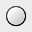
\includegraphics[width=8mm]{bilder804-all/inkscape-tool-skapa-cirklar}}

\index{Inkscape!rita cirkel}
\index{Inkscape!rita ellips}
\index{Inkscape!rotera}
\index{Inkscape!skeva}
\index{Inkscape!skala}

\item Tryck ned muspekaren och dra åt valfritt håll någonstans på den tomma sidan, så ritar du upp en cirkel i önskad storlek. Om du håller ned tangenten \xkey{ctrl} blir det en perfekt cirkel och inte en ellips. Om du vill ändra storleken på cirkeln efter att du har ritat den kan du välja verktyget \textbf{Markera och transformera objekt}. Klicka på objektet du vill ändra, så dyker små handtag i form av pilar upp i de fyra hörnen och mitt på de fyra sidorna (se \fref{inkscape-handtag}). Med dessa kan du ändra storleken på objektet. Om du klickar på objektet ytterligare en gång ändras dessa till rotera- och skeva-handtag (se \fref{inkscape-handtag-rotera}). Du kan växla mellan de två lägena genom att klicka på objektet. Experimentera gärna en stund med de olika handtagen, men se till att du till slut har en cirkel som liknar den i \fref{inkscape-boll-1}. För att flytta ett objekt behöver du bara klicka och dra någonstans i objektet. 

\xbildl{bilder804-all/}{inkscape-handtag}{Handtag för att ändra storlek på objekt.}

\xbildl{bilder804-all/}{inkscape-handtag-rotera}{Handtag för att rotera och skeva objekt.}

\item Häftiga hexagoner. Den som har studerat en fotboll vet att den ofta är sydd av sexkantiga bitar. Sådana behöver vi även här -- Inkscape har ett utmärkt verktyg för ändamålet. Välj verktyget \textbf{Skapa stjärnor och polygoner} i verktygslådan till vänster i fönstret.

\index{Inkscape!rita polygon}

\fbox{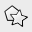
\includegraphics[width=8mm]{bilder804-all/inkscape-tool-skapa-polygoner}}

Kanske lade du nu märke till att en av verktygslisten ovanför ritytan ändrades. Verktygen i verktygslådan har olika alternativ som du kan styra med hjälp av verktygslisten, så även Skapa stjärnor och polygoner-verktyget. 

\xbildw{bilder804-all/}{inkscape-alt-polygoner}{Ställ in hur du vill att verktyget ska fungera i verktygslisten.}

Klicka på knappen \textbf{Vanlig polygon} och stega fram till siffran 6 i menyn \textbf{Hörn}. 

Tryck sedan ned muspekaren och dra åt valfritt håll någonstan på den tomma sidan, så ritar du upp en hexagon i önskad storlek. Klicka på hexagonen med Markera-verktyget och använd handtagen för att ändra storlek och rotera hexagonerna till önskat utseende. Upprepa proceduren tills du har en bild som liknar den i \fref{inkscape-boll-1}.

\xbildl{bilder804-all/}{inkscape-boll-1}{Cirkel och hexagoner: början till en boll.}

\item Du kan ställa in färg både på linjer och fyllning för ett objekt. Ett objekt kan ha valfri bredd på linjerna. Markera först objektet du vill ställa in fyllningsfärg på. Gå till menyn \textbf{Objekt \textgreater{} Fyllning och linje\ldots{}}, så öppnas dialogfönstret Fyllning och linje.

\index{Inkscape!fyllnadsfärg}
\index{Inkscape!linjefärg}
\index{Inkscape!linjetjocklek}

Detta öppnar det flytande fönstret Fyllning och linje (\fref{inkscape-fyllning-linje}. Klicka på fliken \textbf{Fyllning}. Klicka på knappen \textbf{Enfärgad} och kontrollera att fliken \textbf{RGB} är vald. Dra färgreglagen \textbf{R} (röd), \textbf{G} (grön), och \textbf{B} (blå) så långt det går åt vänster (alla ska stå på värdet 0) och färgreglaget \textbf{A} (alfa, genomskinlighet) så långt det går åt höger (värdet 255). Kontrollera också att det övergripande transparensreglaget längst ned i fönstret Fyllning och linje står på 100 procent. Upprepa proceduren för övriga hexagoner.

\xbildw{bilder804-all/}{inkscape-fyllning-linje}{Ställ in fyllning, linjefärg, linjestil med mera.}

\item Nu återstår att fullborda fotbollen genom att knyta ihop hexagonerna med vanliga streck. Välj verktyget \textbf{Rita Bezierkurvor och raka streck} i verktygslådan.

\index{Inkscape!rita streck}
\index{Inkscape!rita Bezierkurva}

\fbox{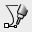
\includegraphics[width=8mm]{bilder804-all/inkscape-tool-rita-vektor}}

Ställ in linjetjockleken genom att gå markera den linje du vill justera och gå till fönstret Fyllning och linje (se \fref{inkscape-fyllning-linje}). Klicka på fliken \textbf{Linjefärg}. Klicka på knappen \textbf{Enfärgad} och kontrollera att fliken \textbf{RGB} är vald. Gör linjen svart på samma sätt som du gjorde med fyllningsfärgen i steget ovanför. Klicka sedan på fliken \textbf{Linjestil} och välj önskad bredd på linjen. 

Klicka på den plats du vill att första strecket ska börja. Klicka sedan på den plats du vill att det ska sluta. Tryck på tangenten \xkey{enter} för att ''avsluta'' strecket. Upprepa proceduren tills du har en bild som liknar \fref{inkscape-boll-2}.

\xbildl{bilder804-all/}{inkscape-boll-2}{En fotboll? Hmm \ldots{} inte riktigt än.}

%\item Vi lägger till någon grad av realism med hjälp av en gradient i cirkeln. Markera cirkeln och gå återigen till fönstret Fyllning och linje (\fref{inkscape-fyllning-linje}. Klicka på fliken \textbf{Fyllning}. Klicka på knappen \textbf{Linjär gradient} (motstå lusten att klicka på Radiell gradient just nu, den ger inte önskad skuggeffekt). Detta ger cirkeln en fördefinierad gradient (svart till vitt). Du kan exakt styra vilken del av gradienten som ska synas genom att välja gradientverktyget. 

%\fbox{
\includegraphics[width=8mm]{pics/inkscape-boll-2}}

%Detta visar start- och stoppnoderna för gradienten. Du kan klicka och dra i noderna för att flytta dem till valfri plats, även långt utanför själva objektet. Justera gradienten tills du är nöjd. (Tänk på att en försiktig effekt ofta blir snyggare än om du överdriver.)

\item Vi är inte riktigt färdiga, bollen ser lite märklig ut. Det som återstår är att dölja de delarna av illustrationen som sticker utanför den runda cirkeln. För att göra detta skapar vi en mask, som vi sedan använder som urklippsmall. 

Urklippet skapar vi i två steg. 

\begin{itemize}

\item Först slår vi ihop alla delar av fotbollen som vi har ritat hittills till en så kallad grupp. När du grupperar ett antal objekt låser du dem i förhållande till varandra. När du roterar, skevar och flyttar gruppen följer alla ingående objekt med -- delarna sitter ihop. Välj verktyget \textbf{Markera och transformera objekt} och klicka och dra en kring alla objekt så att de alla markeras. Gå sedan till menyn \textbf{Objekt \textgreater{} Gruppera}. Se \fref{inkscape-gruppera}. 

\xbildw{bilder804-all/}{inkscape-gruppera}{Gruppera alla objekt som du har ritat hittills.}

\item Rita först en ny cirkel ovanför gruppen. Se till att den nya cirkeln har en fyllnadsfärg (det spelar ingen roll vilken) och att den täcker gruppen. Markera sedan både gruppen du nyss gjorde och den nya cirkeln och gå till \textbf{Objekt \textgreater{} Klipp \textgreater{} Sätt}. Se \fref{inkscape-maskera}.

\xbildw{bilder804-all/}{inkscape-maskera}{Klipp bort de oönskade delarna av teckningen med hjälp av en mask.}
	
\end{itemize}

\item Spara ditt mästerverk genom att gå till \textbf{Arkiv \textgreater{} Spara som\ldots{}}. Fyll i fältet \textbf{Namn}, välj filformat \textbf{Inkscape SVG (*.svg)} i rullgardinsmenyn längst ned till höger, samt ange var du vill spara filen. Klicka på \textbf{Spara}, så sparas filen.
 
\end{enumerate}

\xbildl{bilder804-all/}{inkscape-fotboll-klar}{Det blev en fotboll! Bra jobbat!}

\section{Gör en affisch}

När vi nu har börjat bli lite varma i kläderna tycker jag att vi fortsätter och gör en riktig fyrfärgsaffisch i PDF-format, som vi kan skriva ut själva eller skicka till ett tryckeri. För det behöver vi lägga till text samt göra en fungerande layout. Sagt och gjort:

\begin{enumerate}

\item Börja med att lägga till texten. Som vanligt: \textit{less is more}. En gammal formgivningssanning är att man bör vara återhållsam med att blanda typsnitt. Ett typsnitt har åtminstone fyra olika varianter: normal, kursiv, fet och fet kursiv. Den variationen räcker vanligtvis både till rubriker, brödtext, bildtext och annat. Använd hellre ett enda typsnitt än fyra olika. Vi nöjer oss här med det inbyggda standardtypsnittet Sans i fet stil.

Välj verktyget \textbf{Skapa och redigera textobjekt} i verktygslådan till vänster i fönstret.

\fbox{
\includegraphics[width=8mm]{bilder804-all/inkscape-tool-text}}

Klicka någonstans i bilden för att börja skriva in text. (Du kan behöva zooma in med \textbf{Visa \textgreater{} Zooma \textgreater{} Zooma in} för att se texten ordentligt.)

\item Du kan ändra typsnitt och -storlek genom att gå till \textbf{Text \textgreater{} Text och typsnitt}. Detta öppnar fönstret Text och typsnitt (se \fref{inkscape-typsnitt}).

\index{Inkscape!skriva text}

\xbildw{bilder804-all/}{inkscape-typsnitt}{Ställ in typsnitts, storlek, stil, radavstånd och justering.}

\item Finlir och fintar. Om du vill kan du finjustera bollen så att den ser ytterligare lite ut som en riktig boll. Med verktyget \textbf{Redigera slingor via noder} (Edit paths by nodes) kan du ta tag i enstaka noder i hexagonerna och flytta dem för att förstärka perspektivskänslan. Med verktyget \textbf{Markera och transformera objekt} kan du rotera bollen. Du kan också rita dit några enkla ''fartstreck'', så att det ser ut som om bollen slängs in från vänster i affischen. Lägg också till resten av texten -- svara på frågorna vad?, vem?, när? och var? \ldots{} Gräset då? Hur kom det dit? Det är något för dig att bita i själv. Ett tips: testa verktyget Rita Bezierkurvor och raka linjer.

\index{Inkscape!exportera till PDF}

\item Spara som PDF. Om du vill skicka din trycksak till ett tryckeri bör du spara illustrationen i PDF-format. PDF-formatet är numera närmast att betrakta som \textit{lingua franca} i den grafiska branschen, och både Inkscape och Scribus skapar PDF-filer som funkar direkt hos alla moderna tryckerier. Det enda du bör tänka på när du använder PDF-formatet är att objekt med genomskinlighet och/eller suddighet bör göras om till bildpunktsbaserade element \textit{inuti} Inkscape, annars riskerar du att de går förlorade i PDF-exporten. 

\index{Inkscape!spara som SVG}

Gå till \textbf{Arkiv \textgreater{} Spara som\ldots{}}. Istället för Inkscape SVG (*.svg) väljer du \textbf{PDF via Cairo (*.pdf)} i rullgardinsmenyn längst ned till höger. Skriv in \textbf{Namn} och ange var du vill spara filen, klicka sedan på \textbf{Spara}. Detta öppnar ett inställningsfönster, Cairo PDF Output. Kryssa i \textbf{Convert texts to paths} (konvertera texter till slingor; detta gör om typsnitten till slingor så att du slipper krångel med saknade typsnitt hos tryckeriet) och klicka \xok{}. Filen sparas på den angivna platsen.

\xbild{bilder804-all/}{inkscape-pdf}{Kryssa i rutan för att konvertera texter till slingor, så slipper du typsnittskrångel hos tryckeriet.}

\index{Inkscape!exportera till PNG}
\index{bildformat!PNG}

\item När du är klar kan det vara bra att kunna skapa en bildpunktsbaserad variant av logotypen, exempelvis för användning på klubbens hemsida eller i en OpenOffice.org Impress-presentation. Gör så här för att exportera affischen i PNG-format, lämpligt för webbpublicering.

Markera det objekt du vill göra en bildpunktsbaserad kopia av och gå till \textbf{Redigera \textgreater{} Exportera bitmappsbild}. Fönstret Exportera bitmappsbild öppnas. Klicka på knappen \textbf{Markering} (tredje från vänster längst upp). Ställ in önskad storlek och upplösning på bilden under \textbf{Bitmappens storlek} och ange ange var och med vilket namn filen ska sparas under \textbf{Filnamn}. Klicka därefter på \textbf{Exportera}, så sparas en PNG-bild på önskad plats.

\end{enumerate}

\begin{figure}[htb] 
\noindent\fbox{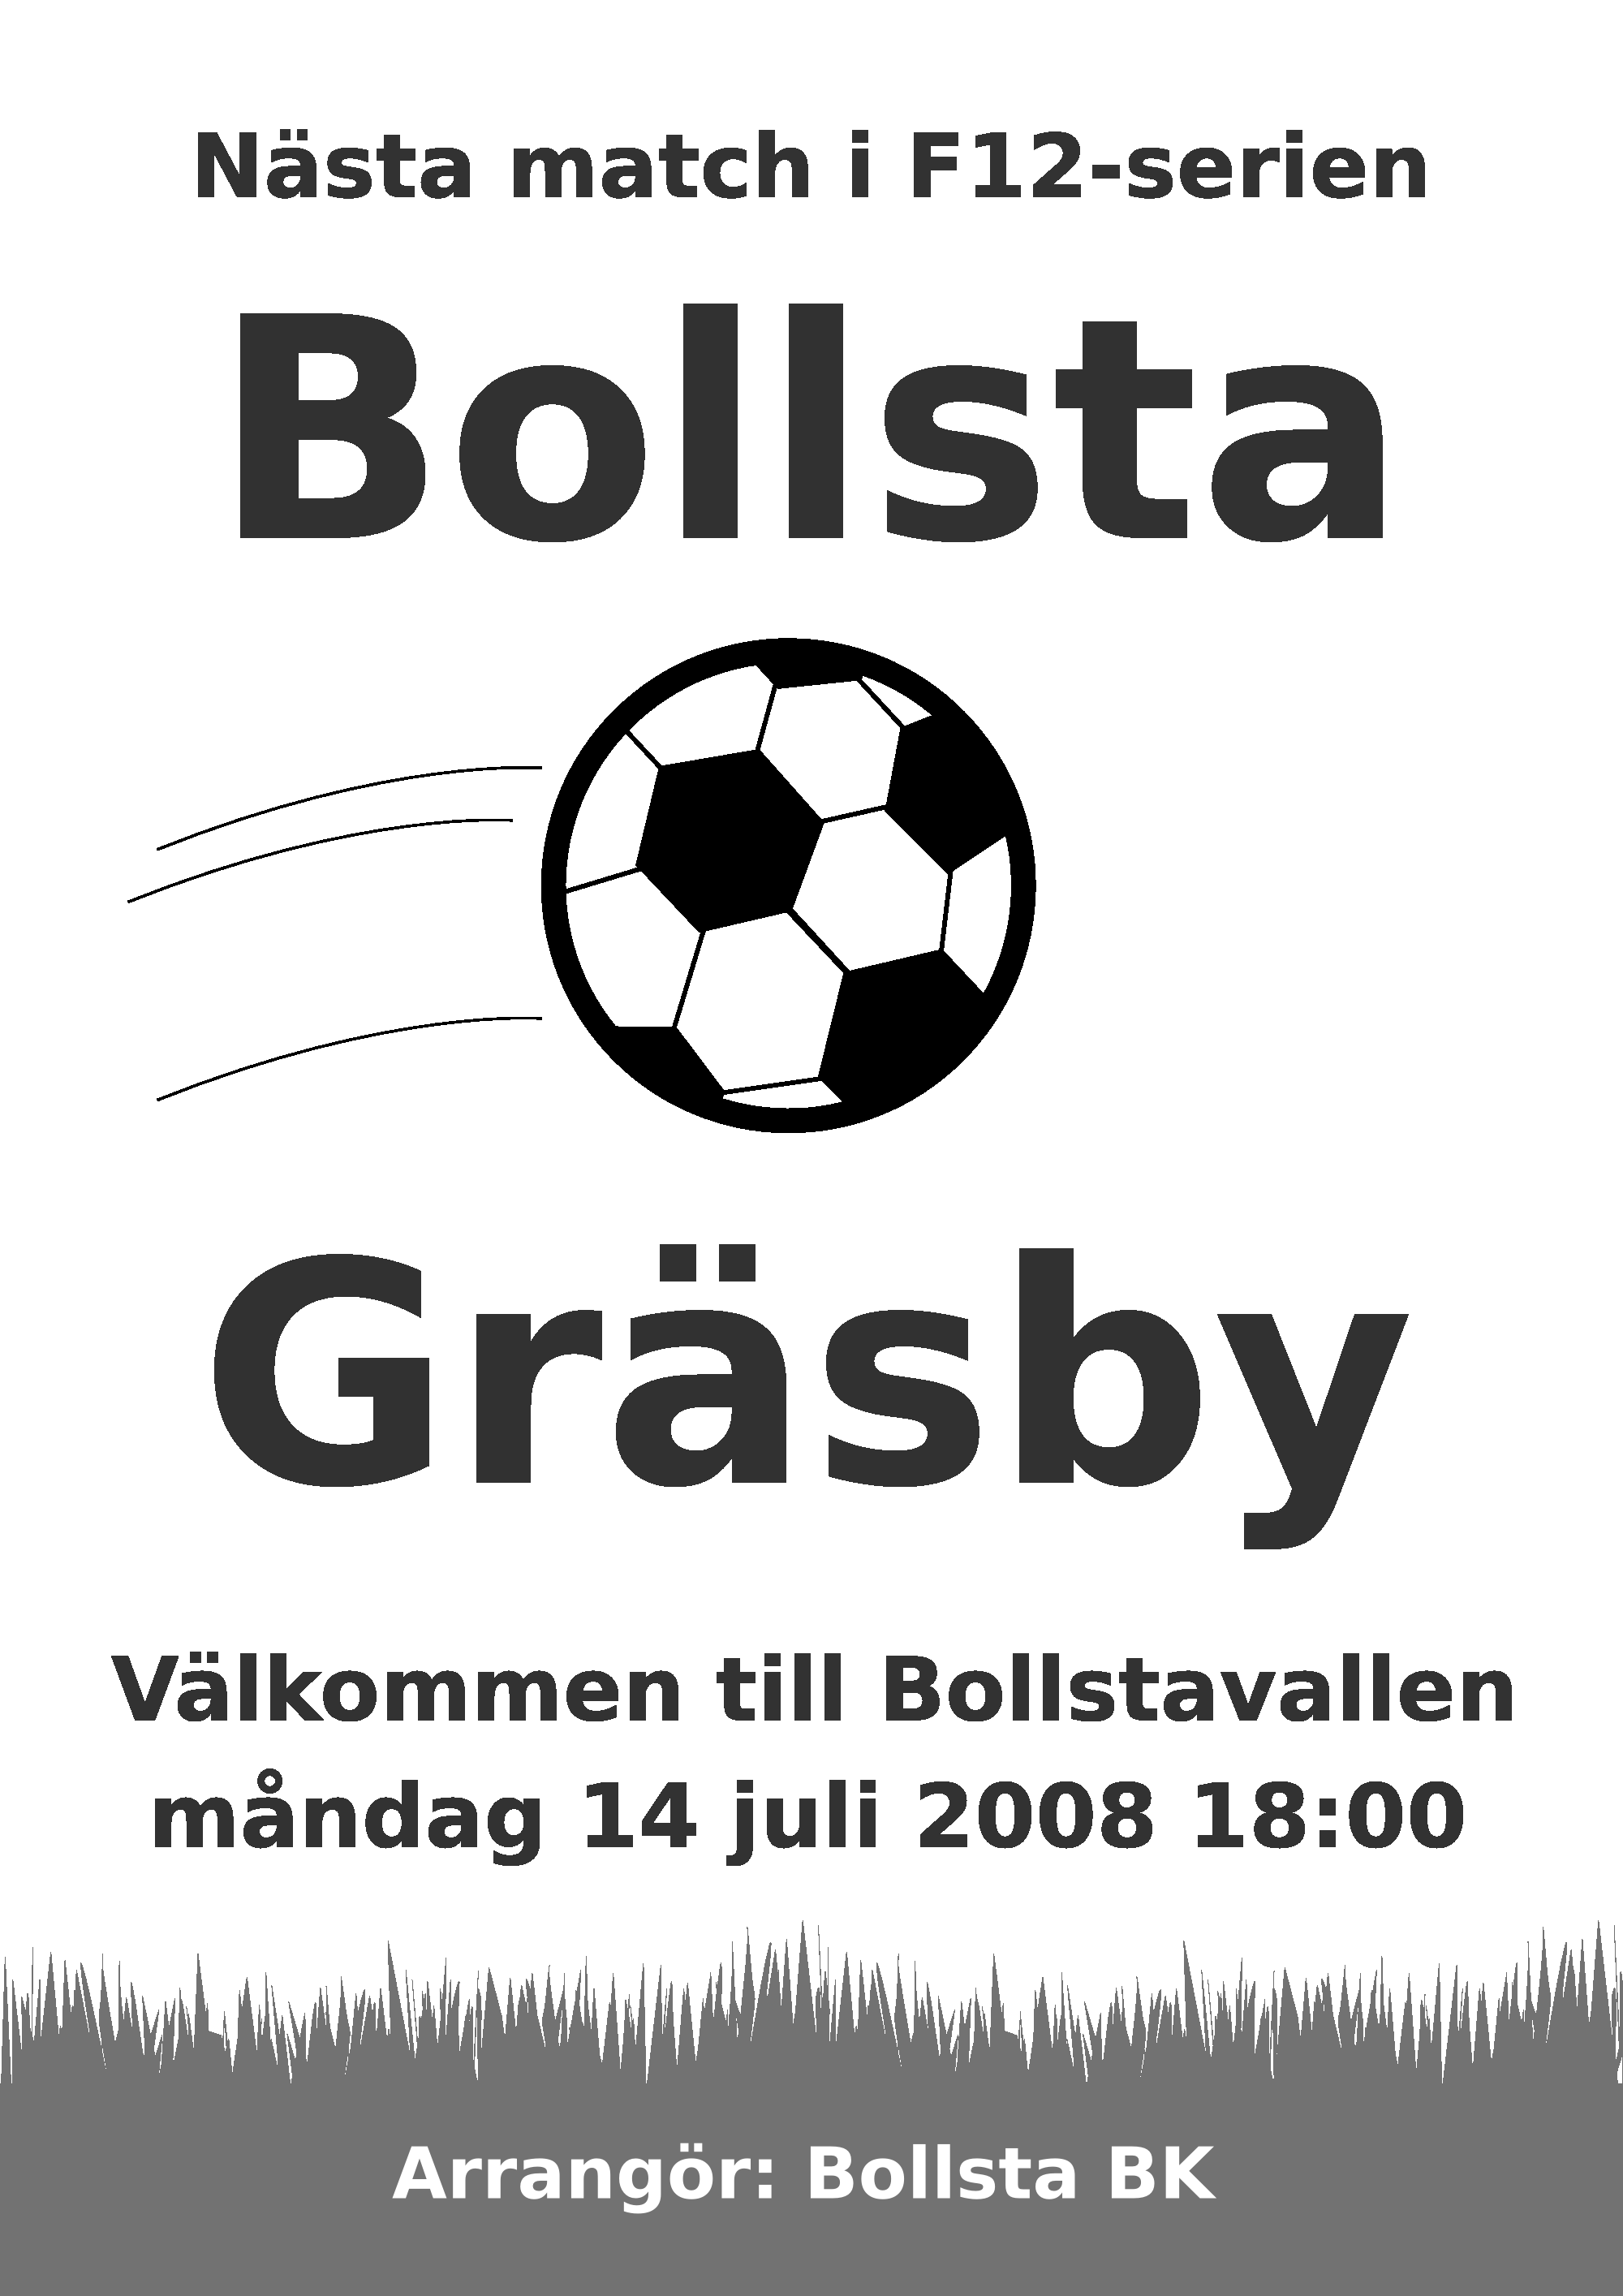
\includegraphics[width=.97\textwidth]{bilder804-all/fotbollsaffisch}}
\smallskip
\caption{Färdig affisch att skriva ut och tejpa upp på byns lyktstolpar.}
\end{figure}

\section{Avancerade tips och tricks (valfritt)}

Inkscape är avancerat nog att ge Adobe Illustrator en match. Du kan på egen hand utforska en mängd avancerade funktioner som gör dina bilder mer realistiska, exempelvis transparens, gradienter och suddighet. Några av de funktioner jag har mest nytt av är följande. Vissa av knepen nedan är ganska avancerade och kräver lite tålamod -- men det är det värt.

\begin{description}

\item[Använda rutnät] Om du vill rada upp objekt prydligt och ordnat kan du slå på ett rutnät, som lägger sig bakom bilden du jobbar med. Slå på rutnätet genom att gå till \textbf{Visa \textgreater{} Stödlinjer}. Om du vill att kanterna på objekt ska sugas fast vid närmaste bakomliggande stödlinje när du jobbar med objektet kan du slå på/av funktionen med \textbf{Visa \textgreater{} Snap}.

\item[Lager] Liksom de flesta andra grafikprogram har Inkscape stöd för lager. Gå till \textbf{Lager \textgreater{} Lager\ldots{}} för att öppna ett dialogfönster som du kan använda för att skapa nya lager, flytta dem upp och ned och visa/gömma dem.

\item[Kalkera bitmappsbilder] Inkscape har en inbyggd funktion för att automatiskt kalkera av bildpunktsbaserade bilder. Du kan använda den genom att skanna en en bildpunktsbaserad bild, importera den till ett Inkscape-dokument med \textbf{Arkiv \textgreater{} Importera}, markera din importerade bilden och därefter gå till \textbf{Slinga \textgreater{} Kalkera bitmappsbild}. Detta öppnar fönstret Kalkera bitmappsbild. Experimentera med inställningarna och förhandsgranska resultatet genom att trycka på knappen \textbf{Update}. När du är nöjd kan du klicka på \xok{} -- så gör Inkscape en vektorvariant av din bild. Mycket smidigt, eller hur?

\item[Justera och distribuera] Under menyalternativet \textbf{Objekt \textgreater{} Justera och distribuera} gömmer sig ett otroligt användbart litet dialogfönster. Med det kan du justera och distribuera objekt relativt varandra på ett mycket smidigt sätt. Öppna dialogrutan och se efter själv, den är lika kraftfull som enkel att förstå sig på.

\item[Klona] Om du vill använda flera kopior av ett objekt i en bild (vilket är ett mycket vanligt sätt att spara tid när man jobbar med exempelvis dekorelement i en illustration) kan du klona objektet med hjälp av \textbf{Redigera \textgreater{} Skapa länkad kopia \textgreater{} Skapa klon}. När du redigerar originalet uppdateras också alla länkade kloner! Du kan till och med automatiskt skapa valfritt antal kopior i ett svep med dialogfönstret Skapa kloner som brickor, under \textbf{Redigera \textgreater{} Skapa länkad kopia \textgreater{} Skapa klon}. Dialogfönstret är lite klurigt att greppa, men experimentera och och fundera, så kommer du kan du bli en supereffektiv illustratör.

\item[Kolla inställningarna] Under \textbf{Arkiv \textgreater{} Inkscape Inställningar} kan du hitta en uppsjö olika inställningar som gäller för Inkscape och alla dokument du skapar i det. Här är det lätt att förlora sig i alla detaljer. Menyalternativet \textbf{Arkiv \textgreater{} Dokumentinställningar} ger dig däremot en bra och koncis sammanfattning av de flesta viktiga inställningarna som du kan behöva göra för ett specifikt dokument, bland annat måttenheter och om du vill att objekt ska sugas fast vid stödlinjer, rutnät och varandra när du för dem nära ett sådant element.

\end{description}

\xtip{Om du vill läsa på mer om Inkscape finns en hel del dokumentation på \url{http://www.inkscape.org/doc/index.php}. På \url{http://tavmjong.free.fr/INKSCAPE/MANUAL/html/} finns också en handledning till Inkscape, skriven av Tavmjong Bah.}

\index{Inkscape|)}
\index{SVG|)}
\index{bildformat!SVG|)}

\xchapter{bilder804-all/Spela_spel_med_tux}{Spela spel på datorn}\label{cha:spel}

\index{spel|(}

\xintro{Antalet riktigt bra spel på Linux växer sakta men säkert. Här är några av de allra bästa, som vart och ett håller hög klass. Det går lika bra att fördriva tid i Linux som i Windows \ldots{}}

\section{Inbyggda klassiska spel}

Med GNOMEs inbyggda spel behöver du inte sakna något från Windows (inte ens spelet Minesweeper). Här finns en hel drös klassiska spel. Gå till \textbf{Program \textgreater{} Spel}. Där hittar du bland annat Schack, Fyra-i-rad och AisleRiot-patiens, liksom min personliga favorit Mahjong. Och om du gillar sudoku behöver du inte bli besviken. 

\index{Mahjong}\index{Shack}\index{Fyra-i-rad}\index{Patiens}\index{Minesweeper}

\xbildw{bilder804-all/}{spel-mahjong}{Ubuntu har fler klassiska spel än du orkar med -- testa Mahjong till exempel.}

\section{Frozen Bubble}\index{Frozen Bubble}

Frozen Bubble är ett enkelt men lätt beroendeframkallande spel. I alla enkelhet går det ut på att med olikfärgade bubblor skjuta ned andra bubblor med samma färg. Spelplanen liknar den för Tetris, eller Gnometris som den inbyggda varianten i GNOME heter, och precis som för Gnometris är målet att få spelplanen tom. Om spelplanen fylls helt och hållet är spelet förlorat. Tricket är att skjuta bubblorna på så sätt att de spräcker likfärgade bubblor. Om du misslyckas fastnar de istället \ldots{}

\xbildw{bilder804-all/}{spel-frozenbubble}{Spräck bubblorna, så blir du inte mosad.}

Installera spelet genom att gå till \textbf{Program \textgreater{} Lägg till/ta bort\ldots{}}, sök på \textbf{frozen bubble} och installera programmet i enlighet med instruktionerna i \Cref{cha:programinstallation}.

\section{FreeCiv}\index{FreeCiv}

FreeCiv är ett spel som i både upplägg och utseende har många likheter med Sid Meiers klassiska spel Civilization och Civilization II. Ditt uppdrag är att år 4~000 före Kristus leda en stam till välstånd och välmåga, med hjälp av teknisk utveckling, diplomati och krigföring. Under seklernas gång förvärvar din civilisation alltmer kunskaper, vilka ständigt sätts på prov i kraftmätningar mot andra civilisationer. Den civilisation som har slagit ut alla andra civilisationer står kvar som vinnare. 

Du kan spela mot andra med FreeCiv över det lokala nätverket eller nätet. Rekommenderas för dig som gillar strategispel.

\xbildw{bilder804-all/}{spel-freeciv}{Civilization II-kopian FreeCiv.}

Installera spelet genom att gå till \textbf{Program \textgreater{} Lägg till/ta bort\ldots{}}, sök på \textbf{freeciv} och installera programmet i enlighet med instruktionerna i \Cref{cha:programinstallation}.

\section{Battle for Wesnoth}\index{Battle for Wesnoth}

Battle for Wesnoth har släktskap med FreeCiv, men är till skillnad från denna inte en klon eller kopia av ett kommersiellt spel. Battle for Wesnoth är ett originalspel för Linux som på kort tid har blivit mycket populärt -- spelet har ett helt unikt upplägg, mycket välgjort grafik och helt egen bakgrundshistoria. Spelet är dragbaserat (du och motståndarna turas om att utföra drag) och har enkla regler. Världen som spelet utspelar sig i är starkt präglad av fantasy och rollspel. Du kan enkelt ansluta till servrar på nätet där du kan kliva in i nya världar och träffa andra spelare.

Spelet är helt översatt till svenska, med omfattande hjälp och guider inbyggt. Rekommenderas varmt.

\xbildw{bilder804-all/}{spel-wesnoth}{Bygg en armé och erövra Wesnoth-världen. Battle for Wesnoth är ett fascinerande fantasifyllt strategispel. Akta dig för orcherna!}

Installera spelet genom att gå till \textbf{Program \textgreater{} Lägg till/ta bort\ldots{}}, sök på \textbf{wesnoth} och installera programmet i enlighet med instruktionerna i \Cref{cha:programinstallation}.

\section{Planet Penguin Racer (3D)}\index{Planet Penguin Racer}

Planet Penguin Racer är ett enkelt men kul 3D-spel med Linuxmaskoten Tux som huvudperson (du måste ha ett relativt nytt grafikkort för att kunna spela spelet, eftersom det kräver att grafikkortet klarar av 3D-grafik). I Planet Penguin Racer tävlar Tux mot klockan i utförsåkning à la pingviner, det vill säga hasandes på mage. För att komma vidare till nästa bana måste du åka snabbt, svänga rätt och fånga många sillar (eller om det nu är strömming).

\xbildw{bilder804-all/}{spel-tuxracer}{Hur många sillar hinner du ta? Det gäller att hitta rätt spår i banan.}

Planet Penguin Racer är en vidareutveckling av det på Linux klassiska 3D-spelet Tux Racer. Prova också varianten Extreme Tux Racer, som är en snarlik variant av Tux Racer.

Installera spelet genom att gå till \textbf{Program \textgreater{} Lägg till/ta bort\ldots{}}, sök på \textbf{planetpenguin} (eller \textbf{extremetuxracer}) och installera programmet i enlighet med instruktionerna i \Cref{cha:programinstallation}.

\section{OpenArena (3D)}\index{Open Arena}

3D-spelet OpenAreana bygger på samma spelmotor som Quake III Arena (det krävs att du har ett modernt grafikkort och en drivrutin för kortet som stödjer 3D för att spelet ska gå att spela). Liksom Quake är det ett \xeng{First Person Shooter}-spel, det du ser på skärmen är det som rollfiguren ser. Spelet är våldsamt adrenalinhöjande och bygger på att du med olika skjutvapen försöker oskadliggöra motståndarna i ett virrvarr av rum, schakt och korridorer.

Installera spelet genom att gå till \textbf{Program \textgreater{} Lägg till/ta bort\ldots{}}, sök på \textbf{openarena} och installera programmet i enlighet med instruktionerna i \Cref{cha:programinstallation}.

\section{Hitta fler Linuxspel}

Det snabbaste sättet att leta efter fler spel är att gå till \textbf{Program \textgreater{} Lägg till/ta bort\ldots{}}. Klicka på kategorin \textbf{Spel} i fönstret som öppnas, så ser du alla spel som finns tillgängliga. Installera de önskade spelen med hjälp av instruktionerna i \Cref{cha:programinstallation}.

\section{Windowsspel}

Om du har ett Windowsspel som du vill fortsätta kunna spela har du flera alternativ, även om alla är en hel del krångligare att komma igång med. Det finns flera alternativ för dig som vill kombinera Ubuntu med Windowsspel.

\begin{enumerate}

\item Installerar du Windows parallellt med Linux (se \Sref{sec:dualboot}), så att du kan starta om datorn med Windows när spellusten slår till. Detta alternativ är det bästa om du vill spela Windowsspel med 3D-grafik.

\item Använd en virtuell maskin (se \Cref{cha:virtualbox}) med Windows i, parallellt med Linux. 3D-prestandan blir lidande eftersom VirtualBox ännu inte har stöd för accelererad 3D-grafik. 

\item Ett alternativ som inte kräver att du startar om datorn är att du installerar Windowskompatibilitetslagret Wine, som gör att du kan köra många Windowsprogram direkt i Linux utan att du behöver äga en Windowslicens eller installationsskiva från Microsoft. Mer information om Wine finns på \url{https://help.ubuntu.com/community/Wine}. 

\item Ännu ett alternativ är Cedega, som är anpassat för snabb 3D-grafik men som är helt kommersiellt. Med Cedega kan du installera de flesta en mängd Windowsspel, exempelvis Battlefield 2142, Oblivion, World of Warcraft, Civilization IV och Madden 2007. Du kan köpa en Cedega-licens från GGS-Data, \url{http://www.ggsdata.se}.

\end{enumerate}

\index{spel|)}

\xchapter{bilder804-all/Kor_flera_OS_Virtualbox}{Kör flera operativssystem samtidigt med VirtualBox}\label{cha:virtualbox}

\index{VirtualBox|(}
\index{virtualisering|(}

\xintro{Varför välja när man kan ha allt? Om du ibland vill kunna starta Windows eller något annat operativsystem samtidigt som Ubuntu är igång kan du använda dig av ett virtualiseringsprogram.}

Med virtualiseringsprogrammet VirtualBox kan du skapa en dator i datorn som du sedan startar ett andra operativsystemet i -- utan att du måste starta om datorn. Inuti den virtuella datorn kan du installera vad du vill: Windows, en andra Ubuntu-maskin, OpenSolaris, eller valfritt annat operativsystem. Skärmen på den virtuella datorn visas som ett vanligt programfönster.

\xbildw{bilder804-all/}{virtualbox-maxat}{Windows XP och Ubuntu i Ubuntu. Med VirtualBox kan du förvandla en dator till flera.}

\section{En kort introduktion}

\index{virtualisering!introduktion|(}

För ett operativsystemet i en virtuell dator (eller virtuell maskin som det ofta kallas) ser den virtuella datorn ut precis som en vanlig dator med grafikkort, ljudkort, hårddisk, minne och processor -- men allt är fejkat av virtualiseringsprogrammet. 

Den virtuella dator kallas gäst och den riktiga datorn som ligger i botten kallas värd.

Gästens virtuella hårddisk består av en skivavbild som ligger på värdens hårddisk. Det gör att du kan flytta en virtuell maskin från en värd till en annan -- du behöver bara kopiera över skivavbilden. En annan fördel med virtualisering är att du får mer valuta datorpengarna, i alla fall om du har en ny snofsig dator med dubbla eller fyrdubbla processorer. Med en eller flera virtuella datorer igång kan alla processorer få jobba!

Andra sofistikerade virtualiseringslösningar av VirtualBox kaliber är antingen krångliga att installera och komma igång med, eller så kostar de en hel del pengar. Företaget VMware erbjuder visserligen en gratisvariant av sitt virtualiseringsprogram, men det är inte fri programvara och har begränsad funktionalitet. I början av 2007 släpptes virtualiseringsprogrammet VirtualBox i en fri källkodsvariant, som numera finns tillgängligt direkt i Ubuntu. VirtualBox OSE (\xeng{Open Source Edition}, fri källkodsutgåvan) har ett smidigt grafiskt gränssnitt för att ställa in och hantera virtuella maskiner.

Fördelen med VirtualBox jämfört med andra fri källkodsvarianter (som exempelvis Xen\footnote{http://www.citrixxenserver.com/Pages/default.aspx} och KVM\footnote{http://kvm.qumranet.com/kvmwiki}) är att det har ett polerat och lättanvänt grafiskt gränssnitt. Det gör det mycket lämpat för hemanvändare som ibland vill kunna köra ett Windowsprogram eller -spel, webbutvecklare som vill testköra sina hemsidor i olika webbläsare på olika plattformar, eller datorintresserade som vill testa olika operativsystem. VirtualBox är i det avseendet precis lika lättanvänt och lika snabbt som gratisversionerna av de icke-fria virtualiseringsprogrammen från VMware (Server respektive Player). 

I den här kapitlet kommer vi gå genom stegen för att att installera ett operativsystem inuti en virtuell dator, helt i enlighet med \textit{learning-by-doing}-filosofin. Utmed vägen stöter du på de mest grundläggande koncepten och handgreppen. När du är klar kommer du själv kunna skapa en ny virtuell dator, konfigurera den, samt installera ett valfritt operativsystem (exempelvis Windows, om du skulle vilja). 

Som exempel använder vi Ubuntus avlägsna lite äldre kusin OpenSolaris, ett fri källkodsvariant av UNIX-operativsystemet Solaris från Sun Microsystems. 

OpenSolaris är del annorlunda än Ubuntu under skalet, men mycket likt på ytan. Istället för kärnan Linux använder OpenSolaris en tidigare helt kommersiell men numera öppnad UNIX-kärna med anor från 1983. För den grafiska miljön använder det dock exakt samma GNOME-gränssnitt som Ubuntu. Det gör det mycket lämpat för detta test: du kommer känna igen dig. Det är bra att hälsa på sina släktingar -- även avlägsna kusiner -- ibland. 

\index{virtualisering!introduktion|)}

\section{Installera och ställ in Virtualbox}\label{sec:virtualboxinstallera}

VirtualBox finns inte installerat från början i Ubuntu, men är enkelt att lägga till. Gå till \textbf{Program \textgreater{} Lägg till/ta bort\ldots{}} och kontrollera att \textbf{Alla tillgängliga program} är valt i rullgardinsmenyn \textbf{Visa}. Sök på \textbf{VirtualBox} och installera programmet i enlighet med instruktionerna i \Cref{cha:programinstallation}.

Innan du kan köra programmet första gången måste du göra två handgrepp på värddatorn: 1) se till att kärnmodulen vboxdrv kan laddas (det är denna drivrutin till Linuxkärnan som gör det möjligt för VirtualBox att skicka vidare gästens kommandon till värdens hårdvara) och 2) lägga till din användare till en speciell användargrupp. 

Dessa saker kan verka krångliga, men följ instruktionerna nedan noggrant så kommer det att gå bra.

\subsection{Installera kärmodulen vboxdrv}

\index{VirtualBox!ställa in|(}

Följande behöver endast göras en gång och kräver att du har en aktiv internetuppkoppling. Stäng VirtualBox OSE-fönstret om du har redan har öppnat det.

\begin{enumerate}

\item Öppna ett Terminalfönster genom att gå till \textbf{Program \textgreater{} Tillbehör \textgreater{} Terminal}.

\item Skriv in följande på raden och avsluta med att trycka på \xkey{enter}:

\texttt{\small sudo apt-get install virtualbox-ose-modules-generic}

\item Du ombeds då skriva in ditt lösenord. Gör det och tryck därefter på \xkey{enter}. 

\item Tryck \xkey{enter} när du får frågan om du vill fortsätta. Detta ber programmet \xcommand{apt-get} att ladda ned och installera den saknade kärnmodulen.

\end{enumerate}

\xtip{I \Cref{cha:kommandoraden} kan du läsa mer om både kommandoraden i allmänhet, liksom om kommandot \xcommand{apt-get}.}

\subsection{Lägg till din användare till gruppen vboxusers}

Även detta behöver du endast göra en gång.

\begin{enumerate}

\item Gå till \textbf{System \textgreater{} Administration \textgreater{} Användare och grupper}. Detta öppnar fönstret Användarinställningar.

\item Klicka på knappen \textbf{Lås upp} längst ned i fönstret. Du ombeds då skriva in ditt lösenord. Gör det och tryck på \textbf{Autentisera} för att återgå till fönstret.

\item Klicka på knappen \textbf{Hantera grupper}, vilket öppnar fönstret Grupp\-inställningar.

\item Rulla ned i listan av grupper tills du hittar \textbf{vboxusers}. Dubbelklicka på namnet, så öppnas fönstret Egenskaper för gruppen ''vboxusers''.

\item Kryssa för ditt eget namn i listan \textbf{Gruppmedlemmar} och klicka på knappen \textbf{OK}.

\item Klicka på \textbf{Stäng} för att stänga fönstret Gruppinställningar och sedan återigen på \textbf{Stäng} för att stänga fönstret Användarinställningar.

\end{enumerate}

Slutligen måste du logga ut och sedan logga in igen för GNOME ska upptäcka ändringarna av gruppinställningarna. Gå till \textbf{System \textgreater{} Avsluta\ldots{}} och välj \textbf{Logga ut}, så kommer du till inloggningsskärmen. Väl där loggar du in igen som vanligt. 

Puh! Nu är vi redo att äntligen sätta igång!

\index{VirtualBox!ställa in|)}

\section{Skapa en ny virtuell dator}

\index{VirtualBox!skapa ny dator|(}

Om du installerade och ställde in VirtualBox i enlighet instruktionerna i \Sref{sec:virtualboxinstallera} kan vi sätta igång med skapandet av en ny virtuell maskin.

\begin{enumerate}

\item Gå till \textbf{Program \textgreater{} Systemverktyg \textgreater{} VirtualBox OSE}. Detta öppnar programmet kontrollfönster (se \fref{virtualbox-start}).

\xbildw{bilder804-all/}{virtualbox-start}{Du kan installera valfritt antal virtuella datorer i din dator med Virtualbox.}

\item Klicka på knappen \textbf{Ny}. Detta öppnar sidan Skapa ny virtuell maskin.

\item Klicka på knappen \textbf{Nästa} för börja skapa den nya maskinen. Du kommer då till sidan Namn och operativsystem.

\item Skriv in ett valfritt namn på maskinen i fältet \textbf{Namn} och välj alternativet \textbf{Solaris} i rullgardinsmenyn \textbf{Operativsystem}. Klicka på \textbf{Nästa}, så kommer du till sidan Minne. 

\item Flytta reglaget \textbf{Basminnesstorlek} till den önskade storleken på den virtuella datorns arbetsminne (RAM), eller skriv in det i rutan till höger om reglaget. Om du installerar OpenSolaris, Windows XP eller en Linuxvariant rekommenderas 512~MB eller mer. Om du installerar Windows Vista rekommenderas minst 1~000~MB (1~GB). Dubbla samtliga rekommendationer om du vill att den virtuella datorn ska fungera riktigt optimalt. Eftersom den virtuella datorn lånar sitt arbetsminne från Ubuntudatorns riktiga RAM-minne behöver du se till att det åtminstone finns lika mycket minne kvar till värddatorn. Bästa prestanda får du om du delar upp arbetsminnet solidariskt mellan värden och gästen (eller gästerna). Klicka på \textbf{Nästa}, så landar du på sidan Virtuell hårddisk.

\item Här kan du skapa en ny virtuell hårddisk för din nya virtuella maskin (som är egentligen är en enkel skivavbild i Ubuntu) genom att klicka på knappen \textbf{Ny\ldots{}}, alternativt välja en eventuell befintlig avbild i rullgardinsmenyn \textbf{Uppstartshårddisk (primär master)}. Om du väljer att skapa en ny hårddisk öppnas guiden Skapa ny virtuell disk. Gör då följande:

\begin{itemize}

\item Klicka på \textbf{Nästa} för att börja skapa hårddiskavbilden.

\item Välj typen \textbf{Dynamiskt växande avbild} i rutan \textbf{Avbildstyp}. (Du kan välja alternativet \textbf{Avbild med fast storlek} om du vill, då blir prestandan aningen bättre, men å andra sidan tar den virtuella hårddiskavbilden mer plats på din hårddisk.) Klicka \textbf{Nästa} så öppnas sidan Plats och storlek för virtuell disk.

\item Skriv in ett namn i fältet \textbf{Filnamn för avbild} och ange en storlek på hårddisken med reglaget \textbf{Avbildsstorlek}. Ange en storlek på minst 10~GB, gärna ännu större för att få plats att jobba med filer på den virtuella hårddisken. Om du har valt dynamiskt växande avbild tar skivavbilden ändå inte upp mer plats än nödvändigt. Klicka \textbf{Nästa}, så kommer du till sidan Sammandrag. 

\item Klicka \textbf{Färdigställ} för att avsluta guiden och återgå till sidan Virtuell hårddisk i guiden Skapa ny virtuell maskin.

\end{itemize}

\item Kontrollera att den nya skivavbilden är vald i rullgardinsmenyn \textbf{Uppstartshårddisk (primär master)} och klicka på \textbf{Nästa} för att se sista sidan, Sammandrag.

\item Klicka på \textbf{Färdigställ}, varpå guiden Skapa ny virtuell maskin stängs. Du ser åter VirtualBox kontrollfönster, med den nya maskinen tillagd i den vänstra ramen. Här samlas alla virtuella maskiner som du skapar. Du kan skapa hur många virtuella datorer som helst (men du kan förstås inte ha ett obegränsat antal igång samtidigt, värdens prestanda sätter stopp för hur många du kan köra åt gången).

\end{enumerate}

Grattis, nu har du skapat en virtuell dator-i-datorn, som du kan installera ett nytt operativssystem i. 

\index{VirtualBox!skapa ny dator|)}

\section{Ställa in en virtuell dator}

Innan vi börjar installationen av OpenSolaris måste du ladda ned en skivavbild. Precis som Ubuntu-installationsskivan kan man starta operativsystemet direkt från skivan (en så kallad \textit{live-cd}), vilket gör den till ett utmärkt alternativ för att testa VirtualBox med -- du kommer igång med den virtuella datorn direkt.

Börja med att gå till \url{http://www.opensolaris.com/get} och klicka på nedladdningslänken. Nedladdningen är helt gratis, OpenSolaris är precis som Linux ett fritt operativsystem. Spara skivavbilden på hårddisken. Du behöver inte bränna den till en cd-skiva, vi kommer använda den som den är i den virtuella datorn.

Det som återstår är att tala om för VirtualBox att den virtuella datorn ska använda skivavbilden du laddade ned för installationen. Gör så här:

\begin{enumerate}

\item Klicka på knappen \textbf{Inställningar} i programmets kontrollfönster VirtualBox OSE. Detta öppna fönstret Inställningar.

\item Vi börjar med att ställa in den virtuella datorn att använda skivavilden. Välj alternativet \textbf{CD/DVD-ROM} i den vänstra ramen.

\item Kryssa i \textbf{Montera CD/DVD-enhet} och välj alternativet \textbf{ISO-avbildsfil}. Klicka sedan på den gula lilla mappknappen till vänster om rullgardinsmenyn, så öppnas fönstret Virtuell diskhanterare som du kan använda för att lägga till skivavbilden.

\xnote{Om du istället väljer alternativet \textbf{Värdmaskinens CD/DVD-enhet} kan du installera direkt från en skiva i datorns cd- eller dvd-enhet. Detta är praktiskt om du exempelvis installerar Windows från en skiva.}

\item Klicka på knappen \textbf{Lägg till} uppe till vänster, vilket öppnar filbläddraren Välj en CD/DVD-ROM-diskavbildsfil. Bläddra dig fram till och markera filen du laddade ned ovan och klicka därefter på \textbf{Öppna}. Detta tar dig åter till fönstret Virtuell diskhanterare.

\item Markera den skivavbild som du nyss lade till och klicka sedan på knappen \textbf{Välj} för att återgå till fönstret Inställningar.

\item Klicka på \textbf{OK} för att stänga fönstret Inställningar.

\end{enumerate}

Nu är vi redo att starta ett nytt operativsystem.

\section{Starta en virtuell dator}

\index{VirtualBox!installera i virtuell dator|(}

Nu är allt klart för att starta den virtuella datorn. Se till att önskad virtuell dator är vald i den vänstra ramen i fönstret VirtualBox OSE och klicka på knappen \textbf{Starta}. Detta öppnar ett nytt fönster med den virtuella datorns skärm.

Om du följde instruktionerna ovan startar datorn med OpenSolaris. När OpenSolaris har laddat klart kommer du till ett skrivbord som är mycket likt Ubuntuskrivbordet -- precis som Ubuntu använder OpenSolaris fönstermiljön GNOME. Du bör känna igen dig i det mesta.

Du kan börja utforska OpenSolaris-skrivbordet, GNOME och alla menyer genom att helt enkelt klicka någonstans i det virtuella datorfönstret. När du interagerar med gästoperativsystemet tar det över musen och tangentbordet. Tryck på den högra \xkey{ctrl}-tangenten för att återge värden kommandot över musen och tangentbordet (se \Sref{sec:virtualbox-anvanda} för information om hur du kan ställa in gästen för att slippa detta). 

Kanske har du lagt märke till att OpenSolaris live-skiva liksom Ubuntu lägger till en installationsikonen på skrivbordet. Klicka på den för att starta installationen av OpenSolaris permanent i den virtuella datorn. 

Installationen är enkel att genomföra, följ bara stegen på skärmen tills du ombeds starta om datorn. 

Gör följande efter avslutad installation av operativsystemet:

\begin{enumerate}

\item Gå då direkt till \textbf{Maskin \textgreater{} Stäng\ldots{}} för att stänga av den virtuella datorn helt. Fönstret Stäng virtuell maskin öppnas.

\item Välj alternativet \textbf{Stänga av maskinen} (alternativet sist i listan) och klicka på \textbf{OK}. Detta stänger av maskinen.

\item Klicka på knappen \textbf{Inställningar} i kontrollfönstret VirtualBox OSE och välj \textbf{CD/DVD-ROM} i den vänstra ramen.

\item Välj alternativet \textbf{Värdmaskinens CD/DVD-enhet}, så är inte längre installationsskivan inkopplad. Detta gör att datorn från och med nu startar från den virtuella hårddisken istället för skivavbilden. 

\item Klicka på \textbf{OK} för att stänga fönstret Inställningar.

\end{enumerate}

Klart!

Nu kan du starta och använda din nya virtuella dator efter eget behag.

\index{VirtualBox!installera i virtuell dator|)}

\section{Använda VirtualBox}\label{sec:virtualbox-anvanda}

Det kan till en början vara lite förvirrande att jonglera med flera operativsystem samtidigt. Läs på om följande, så blir det enklare att använda VirtualBox.

Överst i fönstret finns en menyrad. Med denna menyrad kan du kontrollera den virtuella dator. I menyn \textbf{Maskin} finns ett antal val, bland annat följande:

\begin{description}

\item[\textbf{Helskärmsläge}] Välj detta om du vill att den virtuella datorn ska ta över hela skärmen. När du är i helskärmsläget och vill återgå till det normala läget trycker du \xkeycombination{\xkey{ctrl}+\xkey{f}}. Om använder en gäst som inte har installerat stöd för så kallade Guest Additions (se \Sref{virtualbox-additions}) kan gästfönstret visas med svarta sorgkanter runtom. För att ändra storleken på gästfönstret så att det täcker hela bildskärmsytan måste du ändra bildskärmsupplösning i gästen, med den metod som gästen tillhandahåller. Om du ökar upplösningen blir gästfönstret större, om du sänker upplösningen blir det mindre.

\item[\textbf{Starta om}] Startar direkt om datorn utan att fråga först. Motsvarar att rycka ur elsladden ur en vanlig dator, sedan sätta tillbaka den och starta datorn på nytt. Bör undvikas i alla andra fall än när datorn har hängt sig, eftersom den abrupta nedstängningen kan leda till problem och/eller dataförlust i den virtuella maskinen.

\item[\textbf{Justera fönsterstorleken}] Anpassar skärmfönstret för gästen så att det exakt passar bildskärmsupplösningen i gästen.

\item[\textbf{Ändra automatisk storlek på gästvisning}] Om du har installerat stöd för Guest Additions (se \Sref{virtualbox-additions}) kan du i vissa fall använda den här funktionen för att automatiskt ändra bildskärmsupplösning i gästen. Om gästen inte har Guest Additions installerat gör detta alternativ inget alls. När du använder Ubuntu Linux som gäst fungerar inte heller funktionen.

\item[\textbf{Spara ögonblicksbild\ldots{}}] VirtualBox har många avancerade funktioner som annars bara återfinns i dyra kommersiella program. Ett exempel är funktionen \textbf{Ögonblicksbilder}, vilket låter dig spara frysta ögonblicksversioner av din virtuella maskin. Du kan senare återgå till en sparad ögonblicksbild, vilket är särskilt bra om du kör Windows. Genom att återgå till en tidigare ögonblicksbild kan du mycket snabbt återställa datorn till ett fungerande skick även om du råkar få virus eller spionprogram på maskinen.

\item[\textbf{Stäng\ldots{}}] Om du väljer detta alternativ öppnas fönstret Stäng virtuell maskin, i vilket du har tre alternativ för nedstängning. Det första alternativet, \textbf{Spara maskintillståndet} säger åt VirtualBox att frysa det aktuella tillståndet (inklusive öppna program och dokument) i gästen och sparar ned det på värdens hårddisk. Nästa gång du startar gästen kan VirtualBox tina upp gästen så att du kan fortsätta jobba med det du höll på med tidigare. Detta är ett mycket smidigt sätt att starta och stoppa gäster. Det andra alternativet, \textbf{Skicka avstängningssignal} skickar bara vidare avstängningssignalen till gästen, som sedan själv påbörjar en ordnad, säker, nedstängning. Det tredje alternativet, \textbf{Stänga av maskinen}, motsvarar ett brutalt strömavbrott till gästen, som om du drog ut elsladden till en dator. Alternativ ett eller två rekommenderas, undvik alternativ tre för andra fall än när gästen har hängt sig.

\end{description}

\subsection{Fånga och släppa muspekar- och tangentbordsfokus}

\index{VirtualBox!Guest Additions |(}

När du klickar i gästfönstret efter att ha startat en virtuell dator dyker det upp ett fönster som upplyser dig om att du har alternativet \textbf{Fånga tangentbordet automatiskt} påslaget. Det betyder att när du klickar i gästfönstret ger du gästen kontroll över muspekaren och tangentbordet. När du använder musen eller skriver med tangentbordet är det inuti gästoperativsystemet som det registreras.

Om du vill att gästen ska släppa taget om musen och tangentbordet trycker du på den så kallade värdtangenten. Värdtangenten är som standard inställd att vara höger \xkey{ctrl}-tangent.

Om du vill att VirtualBox automatiskt ska släppa taget om musen när du för muspekaren till och över kanten på gästfönstret måste du installera VirtualBox Guest Additions (se \Sref{virtualbox-additions}).

\subsection{Använda VirtualBox Guest Additions}\label{virtualbox-additions}

VirtualBox Guest Additions är mjukvara som du kan installera inuti en Windows- eller Linux-gäst. Detta ger bland annat stöd för en enda muspekare som du kan röra fritt mellan både värden och gästen utan att behöva använda värdtangenten \xkey{ctrl}, bättre grafikstöd och andra finesser. Starta gästen i VirtualBox och gör sedan följande i gästen (ej i värden):

\subsubsection{Windows som gäst}

\begin{enumerate}

\item Gå till \textbf{Enheter \textgreater{} Installera Guest Additions\ldots{}} i fönstret VirtualBox OSE. Detta monterar automatiskt en cd-avbild i Windows-gästen som innehåller ett installationsprogram, som startar automatiskt. Se \fref{virtualbox-windows}.

\xbildw{bilder804-all/}{virtualbox-windows}{Installera Guest Additions för bättre grafikstöd och sömlös muspekarintegration.}

\item Följ instruktionerna i installationsprogrammet.

\item Ett tag in i installationsprogrammet dyker ett fönster upp som varnar för att mjukvaran du försöker installera inte har genomgått Microsofts testprogram. Klicka på \textbf{Fortsätt ändå}.

\item När installationsprogrammet är klart säger det åt dig att du måste starta om datorn för att slutföra installationen. Välj \textbf{Reboot now} (starta om nu) och klicka på \textbf{Finish} (avsluta).

\end{enumerate}

Så där ja, bra jobbat. När gästen har startat om kan du fritt ändra storlek på gästfönstret, varpå Windows automatiskt ändrar sina bildskärmsupplösning för att exakt matcha fönsterstorleken. Du behöver inte heller frikoppla musfokus med värdtangenten, utan kan fritt flytta muspekaren mellan värd och gäst.

\subsubsection{Ubuntu Linux som gäst}

Om du kör Ubuntu Linux \xubuntuver{} som gäst i VirtualBox kan du installera Guest Additions direkt från Ubuntus förråd. 

\begin{enumerate}

\item Öppna ett Terminalfönster genom att gå till \textbf{Program \textgreater{} Tillbehör \textgreater{} Terminal}.

\item Skriv in följande (allt på en och samma rad) och avsluta med att trycka på \xkey{enter}:

\texttt{sudo apt-get install \\\hspace*{\baselineskip} virtualbox-ose-guest-modules-generic \\\hspace*{\baselineskip}  virtualbox-ose-guest-utils}

\item Du ombeds då skriva in ditt lösenord. Gör det och tryck därefter på \xkey{enter}. 

\item Tryck \xkey{enter} när du får frågan om du vill fortsätta. Detta ber programmet \xcommand{apt-get} att ladda ned och installera modulen.

\item Starta om gästen för att aktivera Guest Additions.

\end{enumerate}

Om inte muspekarintegrationen fungerar trots att du gjorde ovanstående kan det bero på att din gäst inte kör VirtualBox egen grafikdrivrutin. Det kan du ändra genom att följa instruktionerna i \Sref{sec:gtk-displayconfig} och välja grafikkortet \textbf{vboxvideo}.

%\subsubsection{Annat operativsystem som gäst}

%Om du har ett annat operativsystem som gäst, som exempelvis en annan Linuxdistribution än Ubuntu, eller OpenSolaris, kan 

\index{VirtualBox!Guest Additions |)}

\subsection{Använda hårdvaruvirtualisering med VT-x/AMD-V}

\index{VirtualBox!VT-x|(}
\index{VirtualBox!AMD-V|(}

Bakom kulisserna vidarebefordrar VirtualBox gästens kommandon till värdens hårdvara. Kruxet med detta sofistikerade datorlurendrejeri är att kan bli väldigt långsamt på grund av de extra stegen i virtualiseringsmjukvaran. Därför har processortillverkarna Intel och AMD i de senaste versionerna av sina processorer byggt in ett särskilt stöd som gör det möjligt för virtualiseringsprogramvara att ''prata'' direkt med hårdvaran. Intel kallar sin teknologi för VT-x eller, AMD kallar sin för AMD-V. VirtualBox har stöd för VT-x och AMD-V, vilket gör en gäst på en värd med en modern processor snabbare -- i alla fall i teorin. VirtualBox i sitt grundutförande är så snabb att det till och med är bättre att lämna VT-x och AMD-V-funktionerna avstängda, enligt uvecklarna av VirtualBox\footnote{http://tombuntu.com/index.php/2007/10/01/should-you-enable-intels-vt-x-in-virtualbox/}. Du kan själv experimentera med att slå på och av stödet i dina virtuella maskiner. Välj det alternativ som funkar bäst.

Om du vill använda stöd för VT-x (eller AMD-V) kan du göra så här:

\begin{enumerate}

\item Klicka på knappen \textbf{Inställningar} i fönstret VirtualBox OSE. Detta öppnar fönstret Inställningar.

\item Välj alternativet \textbf{CD/DVD-ROM} i den vänstra ramen.

\item Välj alternativet \textbf{Allmänt} i den vänstra ramen i fönstret Inställningar. 

\item Klicka på fliken \textbf{Avancerat} och kryssa i rutan \textbf{Aktivera VT-X/AMD-V} i rutan Utökade funktioner. 

\item Klicka på \textbf{OK} för att stänga fönstret Inställningar.

\end{enumerate}

\index{VirtualBox!VT-x|)}
\index{VirtualBox!AMD-V|)}

\subsection{Bra att veta om Windows Vista och Virtualbox}

Eftersom Windows Vista inte innehåller en drivrutin för det virtuella nätverkskort som VirtualBox tillhandahåller måste du installera Windows Guest Additions för att få en fungerande nätverksuppkoppling. Se \Sref{virtualbox-additions} ovan.

\subsection{Läs mer/få hjälp}

\begin{itemize}

\item På \url{http://www.virtualbox.org/wiki/Downloads} kan du ladda ned en manual (på engelska) för VirtualBox. Manualen gäller den icke-fria versionen av VirtualBox, men den är mycket välskriven och överensstämmer med VirtualBox OSE-versionen i nästan allt (den icke-fria har ytterligare några finesser).

\item På \url{http://www.opensolaris.org/help.html} finns mer hjälp och information (på engelska) om hur du använder virtuella datorer i VirtualBox.

\item På \url{http://forums.virtualbox.org/viewforum.php?f=7} finns ett supportforum på engelska där du kan ställa frågor specifikt om VirtualBox på Linux.

\end{itemize}


\index{VirtualBox|)}
\index{virtualisering|)}


\xchapter{bilder804-all/Fler_Smarta_funktioner_i_Gnome}{Fler smarta funktioner i GNOME}\label{cha:referens}

\index{GNOME skrivbordsmiljö|(}

\xintro{Börjar du känna dig varm i kläderna? Vill du lära dig behärska GNOME-skrivbordet till fulländning? Läs vidare.}

\section{Flera funktioner i Nautilus}

I den här sektionen går vi igenom en mängd riktigt användbara funktioner i filbläddraren Nautilus -- bland annat hur du ansluter din dator till Windowsdatorer i ett hemma- eller kontorsnätverk och hur du kan bränna cd- och dvd-skivor med några musklick.

\subsection{Sätta ett emblem på en mapp}

\index{Nautilus!använda emblem|(}

Emblem är en trevlig Linux-unik sak som kan göra det lättare att snabbt visuellt hittat det du söker. Säg att din hemmapp består av en uppsättning mappar för olika ändamål -- en mapp som heter Musik, en annan som heter Bilder, en tredje som heter Privat och så vidare. För var och en av dessa mappar kan du klistra på ett litet märke, eller emblem, som ger en indikation om vad mappen innehåller. Det finns mängder av emblem att välja mellan för ett stort antal ämnen. 


Gör så här för att sätta ett emblem på en mapp:

\begin{enumerate}

\item Gå till din hemmapp genom att gå till \textbf{Platser}-menyn.
\item Leta reda på och högerklicka på den mapp eller fil du vill sätta ett emblem på (om du vill sätta ett emblem på den mapp som du ser innehållet för i Nautilusfönstret kan du högerklicka någonstans på den vita bakgrunden).
\item Välj \textbf{Egenskaper} i menyn. 
\item Öppna fliken \textbf{Emblem} i fönstret som öppnas. Nu ser du alla tillgängliga emblem -- här finns det mesta (se \fref{nautilus-emblem}). 
\item Kryssa i rutan bredvid det eller de emblem du vill sätta på mappen (ja, det går utmärkt att sätta flera emblem på en mapp) och klicka \xstang{} för att stänga fönstret.

\end{enumerate}

\xbild{bilder804-all/}{nautilus-emblem}{Sätt emblem på dina mappar så känner du igen innehållet snabbare.}

\index{Nautilus!använda emblem|)}

\subsection{Ändra behörigheterna för filer och mappar}

\index{Nautilus!filbehörigheter, ändra|(}

I Linux klassificeras användare i tre olika kategorier, som var och en kan ha olika typer av rättigheter att använda filer och mappar. Dessa användarkategorier och rättighetsinställningar används för att bestämma vem som har rätt att läsa och ändra i en viss fil eller köra ett visst program. Det är bland annat det här systemet som gör Linux till ett väldigt säkert operativsystem. En användare på en dator kan inte komma åt andras filer på datorn (om inte användaren har ett administratörskonto, förstås).

Nu lät allt det här säkert ganska krångligt, men läs vidare ändå -- det viktiga här och nu är att du har hört talas om det och att du vet att du kan gå tillbaka hit om du vill fördjupa dig senare. 

De tre olika typerna av användare är följande:

\begin{itemize}
\xitem{Ägaren}{Ägaren till en fil är detsamma som användaren som skapade filen. Om du startar OpenOffice.org Writer, skriver ett brev och sedan sparar det på hårddisken blir du automatiskt ägaren till den filen.}
\xitem{Gruppen}{Varje fil tilldelas också en grupptillhörighet. En grupp är helt enkelt en samling olika användare som delar samma behörighet till en fil. Det som gör vissa användare till administratör av datorn är att han eller hon tillhör administratörsgruppen. (I grundläget tilldelas alla filer som du skapar en grupp med samma namn som ägaren -- din användare har en egen grupp som endast består av dig själv.)}
\xitem{Andra}{Med de andra menas just detta: alla andra.}
\end{itemize}

De olika typer av rättigheter som var och en av användartyperna ovan kan ha är också tre till antalet. De är:

\begin{itemize}
\xitem{Läsa}{Att kunna läsa en fil betyder att du kan komma åt den, öppna den och läsa innehållet.}
\xitem{Skriva}{Att kunna skriva till en fil betyder att du förutom att kunna läsa den också ändra i filen.}
\xitem{Köra}{Den här rättighetstypen avser endast program och avgör om du har rätt att starta programmet eller inte.}
\end{itemize}

De tre olika användarkategorierna kan var och en ha olika uppsättningar rättigheter och kombineras hur som helst. Du som \textit{ägare} till en fil kan ha rätt att både läsa och skriva till den, medans \textit{gruppen} kanske endast har rätt att läsa den och alla \textit{andra} varken har rätt läsa eller skriva till den. 

Tack och lov behöver du som vanlig datoranvändare inte bry dig om allt detta -- Ubuntu, GNOME och Nautilus tar hand om alla smaskiga detaljer bakom kulisserna så att du dag efter dag fortsätter komma åt dina egna filer, alltmedan din retsamma lillasyster inte kan göra det.

Men kanske vill du och din syster faktiskt kunna komma åt vissa gemensamma filer -- kanske ett arkiv fullt med musik som ni har kopierat över från era cd-skivor till datorn. Då kan det vara bra att kunna ändra inställningarna för den mapp och/eller de filer som ni önskar ha gemensam åtkomst till. Då är det bra att känna till hur du kan ställa in det precis så. I Nautilus är det ganska enkelt. Gör så här:

\begin{enumerate}

\item Gå till din hemmapp genom att gå till \textbf{Platser}-menyn.
\item Leta reda på och högerklicka på den mapp eller fil du vill ändra rättigheterna för (om du vill ändra egenskaperna för den mapp som du ser innehållet för i Nautilusfönstret kan du högerklicka någonstans på den vita bakgrunden).
\item Välj \textbf{Egenskaper} i menyn. 
\item Öppna fliken \textbf{Rättigheter} i fönstret som öppnas. Nu ser du alla rättigheter för var och en av de tre användartyperna ägare, grupp och andra (se \fref{nautilus-filrattigheter}). 
\item Ställ in rättigheterna så att de blir som du vill ha dem och klicka \xstang{} för att stänga fönstret.

\end{enumerate}

Ändringarna börjar gälla omedelbart.

\xbild{bilder804-all/}{nautilus-filrattigheter}{Ställ in rättigheterna för filer och mappar i Nautilus.}

\index{Nautilus!filbehörigheter, ändra|)}

\subsection{Ansluta till en Windows- eller Macdator}\label{samba}

\index{Nautilus!Samba|(}
\index{Nautilus!ansluta till Windows-dator|(}
\index{Windows!ansluta till dator|(}

%Linux kan mycket enkelt ansluta till andra datorer på nätverket, oavsett om de kör Linux, Windows eller Mac OS. Det finns flera olika sätt att koppla ihop din dator med andra datorer, men i det här avsnittet koncentrerar vi oss på den metod som är enklast och som fungerar med alla tre datortyper: med mjukvaran Samba. Samba är en fri källkodsvariant av Windows standard för hur datorer pratar med varandra i ett nätverk och finns inbyggt i Nautilus. 

Med Nautilus kan du ansluta din Linux-dator direkt till en Windows-dator, eller din Windows-dator till din Linux-dator. Lika enkelt kan du koppla ihop din Linux-dator med en Mac OS~X-dator och vice versa.

Instruktionerna nedan kräver att du har en Windows- eller Mac-dator inkopplad på ditt hem- eller kontorsnätverk och att du har ett användarkonto med ett lösenord på den datorn. Du måste också ha ställt in datorn så att den accepterar anslutningar utifrån och att du har delat ut åtminstone en mapp på den datorn. 

Gör så här för att ansluta till en delad mapp på en Windows- eller Macdator:

\begin{enumerate}

\item Gå till \textbf{Platser}-menyn och välj \textbf{Nätverk}.
\item Klicka på \textbf{Windows-nätverk}.
\item Du kommer nu att se en eller flera ikoner med namn på dina så kallade domäner (olika grupper av Windowsdatorer). Se exempel i bild \fref{nautilus-bladdra-natverk}.
\item Nu ser du namnet på den eller de datorer som ingår i den valda domänen. Klicka på datornamnet.
\item I det här steget ser du de mappar som är utdelade på den valda datorn. Klicka på den mapp du vill komma åt.
\item I det här steget poppar det upp ett fönster som frågar efter inloggningsnamn och lösenord på datorn du vill ansluta till. Skriv in uppgifterna och klicka på knappen \textbf{OK}.

\end{enumerate}


\xbild{bilder804-all/}{nautilus-bladdra-natverk}{Anslut till ett Windowsnätverk (med Windows-, Mac- eller andra Linuxdatorer).}


Det är allt! Nu öppnas ett fönster som visar innehållet i mappen på den andra datorn i nätverket. Du kan nu fritt kopiera mappar och filer mellan datorerna.

%På \pref{delademappar} får du lära dig hur du ställer in din egen dator så att det går att ansluta till den från andra Windows-, Mac- och Linuxdatorer.

\index{Nautilus!Samba|)}
\index{Nautilus!ansluta till Windows-dator|)}
\index{Windows!ansluta till dator|)}

\subsection{Lägga till ett panelprogram/programstartare i panelen}

\index{panelprogram!lägga till|(}
\index{programstartare!lägga till|(}

I \Cref{cha:programinstallation} fick du lära dig att installera program och lägga till en programstartare för programmet i den övre panelen. Förutom startare till vanliga program kan du lägga till speciella små panelprogram. Exempel på sådana är tid- och datumknappen, batteriindikatorn och ljudvolymsknappen i den övre panelen och papperskorgsikonen i den nedre panelen. Det finns många fler sådana små användbara panelprogram. 

Men vi börjar med ett ytterligare sätt att lägga till just programstartare, både för program som finns i Program-menyn och sådana som inte gör det.

\subsubsection{Lägga till en programstartare}\label{panelprogram-programstartare}

Du kan lägga till en ny programstartare så här:

\begin{enumerate}

\item Högerklicka någonstans på en tom del av panelen och välj alternativet \textbf{Lägg till i panelen\ldots{}} (\fref{programstartare}) i menyn som dyker upp. Detta öppnar fönstret Lägg till i panelen.

\xbild{bilder804-all/}{programstartare}{Lägg till ett panelprogram eller en programstartare genom att högerklicka någonstans på en tom yta i den övre panelen, så öppnas en meny som du kan använda för ändamålet.}

\item I Lägg till i panel-fönstret finns bland annat knappen \textbf{Programstartare\ldots{}}. Klicka på den knappen så visas en lista med alla installerade program på datorn (\fref{panelprogram-programstartare-laggtill}).

\xbild{bilder804-all/}{panelprogram-programstartare-laggtill}{Lägg till en programstartare i den övre panelen för något av de installerade programmen.}

\item Bläddra dig fram till det program du vill lägga till en programstartare för. Markera programmet och klicka \textbf{Lägg till}. Du kan lägga till hur många programstartare som du önskar på det här sättet.

\item Klicka \xstang{} när du är klar.

\end{enumerate}

Använd knappen \textbf{Anpassad programstartare} för att manuellt lägga till en programstartare för ett program som inte finns i Program-menyn på datorn. Då öppnas fönstret Skapa programstartare. Ange \textbf{Namn}, \textbf{Kommando} samt eventuellt en ikon (genom att klicka på knappen \textbf{Ingen ikon} och välja en valfri ikon från listan som visas i fönstret som öppnas) och klicka sedan på \xok{}.

\subsubsection{Lägga till ett panelprogram}\label{panelprogram}

Lägg till ett panelprogram så här:

\begin{enumerate}

\item Högerklicka någonstans på en tom del av panelen och välj alternativet \textbf{Lägg till i panelen\ldots{}} i menyn som dyker upp. Detta öppnar fönstret Lägg till i panelen.

\item I Lägg till i panel-fönstret finns en mängd olika panelprogram (se nedan för mer information om några av dem). Markera det panelprogram som du vill lägga till och klicka på knappen \textbf{Lägg till}.

\item Klicka \xstang{} när du är klar.

\end{enumerate}

Om du vill ändra inställningarna för ett panelprogram kan du högerklicka på ikonen för panelprogrammet och välja \textbf{Inställningar}. För att ta bort ett panelprogram högerklickar du och väljer \textbf{Ta bort från panelen}.

\subsubsection{Några bra panelprogram att välja mellan}

Följande är en lista över några av de panelprogram du kan lägga till utöver de som finns i panelerna från början:

\begin{itemize}

\xitem{Fönsterväljare}{Om du har använt Mac~OS 9 eller tidigare kommer du kanske ihåg att det längst till höger i den övre menyraden fanns en liten smidig meny som man kunde använda för att växla mellan alla öppna fönster. Fönsterväljare är precis ett sådant litet program. Använd det för att snabbt växla mellan öppna fönster.}

\xitem{Låda}{En låda är ett slags anpassningsbar liten meny som kan innehålla precis det du vill: programstartare, andra panelprogram, mappar, dokument\ldots{}. Efter att du har lagt till en låda kan du dra och släppa det du vill till den.}

\xitem{Tvinga avslutande}{Ibland händer det att ett program krånglar, hänger sig och slutar svara på dina kommandon. Det kanske till och med inte går att stänga det. Med det här panelprogrammet kan du klicka bort ett sådant program som annars vägrar göra som du vill. När du har lagt till Tvinga avslutande i panelen kan du klicka på det för att förvandla den vanliga muspekaren till ett kors. Samtidigt visas en kort instruktion (\fref{tvingaavslutande}). Klicka med korset på programmet som trilskas, så elimineras det snabbt och smärtfritt.}\index{tvinga avslutande}

\xbild{bilder804-all/}{tvingaavslutande}{Använda panelprogrammet Tvinga avslutande för att ta kål på ett motvalls program.}

\xitem{Modemövervakare}{Detta panelprogram kan du använda för att aktivera och inaktivera en modemuppkoppling som du har ställt in med fönstret Nätverksinställningar (se \Sref{natverksinstallningar}). Efter att ha installerat panelprogrammet kan du styra uppkopplingen genom att högerklicka på dess panelprogrammets ikon och välja \textbf{Aktivera} eller \textbf{Inaktivera}.}\index{modem!koppla upp/ned}\index{nätverk!modemuppkoppling}

\xitem{Systemövervakare}{Med panelprogrammet Systemövervakare kan du med en små animerade diagram direkt i panelen hålla koll på processorbelastningen, nätverksaktiviteten, hårddiskaktiviteten, systembelastningen och minnesanvändningen -- utan att starta något separat program. I grundläget visas endast processorbelastningen, men du kan enkelt aktivera övervakning av övriga resurser genom att högerklicka på processorövervakare och välja \textbf{Inställningar}.}

\xitem{Övervakare av processorfrekvensskalning}{Många bärbara datorer hushållar med batteriladdningen genom att sänka processorhastigheten när systembelastningen går ner. Detta kallas processorfrekvensskalning. Med panelprogrammet med samma namn kan du se vilken hastighet datorns processor kör i för tillfället.}

\xitem{Fisk}{En fisk som heter Wanda. Prova den så blir allt uppenbart.}

\xitem{Ordboksuppslagning}{Stoppar in ett litet sökfält som du kan mata in ord som du vill få förklarade i. Kräver internetuppkoppling, eftersom panelprogrammet söker efter ordförklaringarna på servrar på nätet. Innehåller huvudsakligen engelska ordböcker.}

\xitem{Tomboy}{Tomboy är en anteckningsbok som du kan använda för att snabbt krafsa ned telefonnummer, saker du vill komma ihåg och vad som helst som faller dig in. Den har en smart funktion som låter dig länka en anteckning till en annan (ungefär som en Wiki på nätet) samt möjlighet att söka i dina anteckningar.}

\xitem{Väderrapport}{Med Väderrapport kan du få senaste väderuppgifterna från en väderstation nära dig (bra om du inte orkar dra upp persiennerna) eller någon annanstans. Ställ in önskad väderstation genom att högerklicka på panelprogrammets ikon och välja \textbf{Inställningar}, klicka på fliken \textbf{Plats} i fönstret som öppna bläddra dig fram till rätt världsdel, land och stad. Klicka sedan \xstang{}. Om du klickar med vänsterknappen på ikonen öppnas ett fönster som heter Detaljer (\fref{vader}). Det innehåller just det -- temperatur, daggpunkt, luftfuktighet, vind, tryck, sikt med mera\ldots{}}

\xbild{bilder804-all/}{vader}{Väderbiten? Missa inga detaljer med panelprogrammet Väderrapport.}

\xitem{Tangentbordsindikator}{Med den här kan du med en knapptryckning växla mellan de olika tangentbordslayouter som du har aktiverat. Se instruktioner för detta på \pref{tangentbordslayout}.}\label{layoutvaxling}

\xitem{Teckenpalett}{Med Teckenpalett kan du snabbt komma åt knepiga tecken som inte finns på tangentbordet, som $\bullet{}$, $\pm$, med flera.}

\end{itemize}

Du kan ta bort en programstartare eller ett panelprogram genom att högerklicka på det och välja \textbf{Ta bort från panelen} i menyn som poppar upp. Likaså kan du flytta ikonen om du högerklickar och väljer \textbf{Flytta}.

\index{panelprogram!lägga till|)}
\index{programstartare!lägga till|)}

\subsection{Växla mellan arbetsytor}\label{arbetsytor-vaxla}

\index{arbetsyta!växla mellan|(}

En av de nya finesserna som Apple marknadsför hårt i den senaste versionen av Mac OS X (kodnamn Leopard) är något som kallas ''Spaces'', med argumentet att det ger användaren ordning och reda i livet. För alla Linuxanvändare är funktionen skåpmat: motsvarande funktion har funnits i Linux sedan urminnes tider (i datorsammanhang i alla fall) och kallas arbetsytor. Tänk på arbetsytorna som separata skrivbord. I verkliga livet kan du ha ett skrivbord i arbetsrummet där du kan bre ut dina jobbprylar, ett annat i gästrummet för symaskinen, ett tredje i garaget som arbetsbänk när du täljer träfigurer\ldots{} och så vidare. 

Med hjälp av funktionen arbetsytor i Linux kan du ha så många skrivbord du behöver. Du kan ha ditt mejlprogram i helfönsterläge på en arbetsyta, webbläsaren på ett andra och en ordbehandlare igång på ett tredje, utan att något av fönsterna skymmer sikten (maximala antalet arbetsytor är betryggande stort -- 36).

\xbildl{bilder804-all/}{arbetsytebytare}{Klicka på arbetsytebytaren för att hoppa mellan dina arbetsytor.}

Ubuntu är förinställt att visa två arbetsytor. Titta längst ned till höger på skärmen. Bredvid papperskorgsikonen i den nedre panelen ser du två rektanglar, som vardera representerar en arbetsyta (se \fref{arbetsytebytare}. Den vänstra rektangeln är förmodligen den du ser på skärmen för närvarande. Klicka nu på den högra. Poff -- nu hoppade du till en ny, tom arbetsyta. Testa nu att öppna ett fönster, till exempel din hemmapp genom att gå till \textbf{Platser \textgreater{} Hemmapp}. Detta öppnar ett Nautilus-fönster som visar innehållet i din hemmapp. Klicka igen på den vänstra rektangeln. Poff igen -- Nautilus-fönstret försvann och du är nu åter på den ursprungliga arbetsytan.

Att växla mellan arbetsytorna är lika enkelt som att klicka med musen. 

\index{arbetsyta!lägga till|(}
\index{arbetsyta!ta bort|(}

\subsubsection{Lägga till/ta bort arbetsytor}

Om du har börjat använda arbetsytor och vill lägga till flera är det enkelt åtgärdat. Högerklicka på någon av arbetsytorna i den nedre panelen och välj \textbf{Inställningar} i menyn som poppar upp. Detta öppnar fönstret Inställningar för arbetsytebytare.

I inmatningsfältet \textbf{Antal arbetsytor} kan du själv ställa in hur många arbetsytor du vill ha. För varje ny arbetsyta du lägger till läggs också en motsvarande rektangel till i panelen. Klicka på \xstang{} när du är klar.

\index{arbetsyta!lägga till|)}
\index{arbetsyta!ta bort|)}
\index{arbetsyta!växla mellan|)}

\subsection{Använda Nautilus inbyggda cd- och dvd-brännare}\label{subsec:burner}

Till skillnad från Windows XP har Linux en inbyggd cd- och dvd-brännare. Den är dessutom föredömligt enkel att använda, även för dig som aldrig tidigare har vågat dig på att bränna en cd- eller dvd-skiva. I Ubuntu Linux behöver du inte installera någon extra mjukvara med en massa avancerade finesser (även om sådana också finns i Linux) för att göra en kopia av en musikskiva, mångfaldiga sommarens semesterfilm på dvd eller bränna en installationsskiva för Linux. Allt finns redan tillgängligt på några musklicks avstånd. Följ med så får du se!

\xnote{Jag rekommenderar att du håller dig à jour med vilka rättigheter du har att kopiera musik och annat enligt upphovsrättslagstiftningen (ett område som för övrigt är föremål för livliga diskussioner just nu). Du får naturligtvis inte kopiera skyddad musik för att sälja den vidare, men du har rätt att göra en kopia av en musik- eller dvd-skiva som du själv har köpt om skiva inte innehåller kopieringsskydd. Om den innehåller något slags tekniskt skydd som ska hindra kopiering får du i grundläget inte kringgå det. Men om en skiva som du har köpt har kopieringsskydd och du vill \textit{spela upp} den i Linux är det däremot enligt svensk lag tillåtet att kringgå kopieringsskyddet. \\\indent På regeringens hemsida, \url{http://www.regeringen.se/sb/d/1920/a/55368}, kan man bland annat läsa följande fråga och svar: ''För att kunna lyssna på cd-skivor med kopieringsskydd i en dator måste man ofta kringgå kopieringsskyddet. Är det olagligt? Nej, det är tillåtet att gå förbi spärrar som hindrar dig från att t.ex. lyssna på en cd-skiva i vilken apparat du vill. Man kan alltså lagligen gå förbi en spärr för att spela upp musik, filmer m.m. på alternativa operativsystem. En förutsättning är dock att man har lovlig tillgång till det exemplar man vill lyssna eller titta på, t.ex. genom att man köpt en cd-skiva.'' \\\indent Mer om upphovsrätt i allmänhet finns på \url{http://www.regeringen.se/sb/d/1910/a/12248}.}

\subsubsection{Bränna filer på en data-cd eller data-dvd}\label{nautilus-burn-data}

\index{Nautilus!bränna data-cd/dvd|(}

Det vanligaste skälet att bränna en skiva är förmodligen för att göra en säkerhetskopia på filer som du har sparat på hårddisken, eller för att kunna flytta filerna till en annan dator. Då är det smidigt att stoppa in en tom cd- eller dvd-skiva, välja ut filerna som ska kopieras och klicka på en knapp -- sedan är skivan klar. 

\xnote{Innan vi börjar: se till att du har tillgång till en tom cd-skiva eller dvd-skiva med minst lika mycket utrymme ledigt som storleken på de filer du vill bränna. Om du vill använda en dvd-skiva måste du kontrollera att den passar med den typ av dvd-brännare som du har. Det finns två slags dvd-skivor. De två typerna kallas -- (brukar stå DVD-R, DVD-RW på förpackningen) och + (DVD+R, DVD+RW). Om din brännare klarar båda slagen spelar det ingen roll vilken du väljer.}

Så här går det till:

\begin{enumerate}
\item Gå till din hemmapp genom att gå till \textbf{Platser}-menyn.
\item Gå till menyn \textbf{Gå \textgreater{} Cd/dvd-skapare}. Fönstret Cd/dvd-skapare öppnas.
\item Dra och släpp de filer du vill bränna på fönstret. Filerna du drar till fönstret flyttas inte från sina ursprungsplatser, de ligger tryggt kvar (se bild \fref{nautilus-cddvdbrannare-filer}).
\item Är du nöjd med innehållet på skivan? Klicka i sådana fall på \textbf{Skriv till skiva}. Detta öppnar fönstret Skriv till skiva.
\item Skriv in ett valfritt namn på din skiva i fältet \textbf{Namn på skiva}, eller låt det förifyllda förslaget vara kvar. Klicka sedan på \textbf{Skriv}. Om du inte redan har stoppat in en tom skiva i din cd-/dvd-enhet poppar det nu upp ett fönster som ber dig göra det.
\item Stoppa i en tom skiva, vänta några ögonblick tills datorn hinner spinna igång skivläsaren och klicka \textbf{OK}. Nu visar ett fönster en statusstapel under tiden som bränningen fortskrider. (Du kan när som helst avbryta bränningen genom att klicka på knappen \textbf{Avbryt}.)
\item När bränningen är klar är statusstapeln full. Du kan då klicka på knappen \xstang{} eller \textbf{Skapa ytterligare en kopia} om du vill göra en kopia till.
\end{enumerate}

\xnegskip\xtip{Om din cd- eller dvd-brännare ofta trilskas och misslyckas med att bränna skivor kan du prova att sänka bränningshastigheten i rullgardinsmenyn \textbf{Skrivhastighet} i fönstret Skriv till skiva. Om bränningen av dina skivor fungerar som det ska behöver du dock inte ändra inställningen.}

\xbild{bilder804-all/}{nautilus-cddvdbrannare-filer}{Bränn cd- och dvd-skivor enkelt och snabbt med den inbyggda funktionen i Nautilus.}

\index{Nautilus!bränna data-cd/dvd|)}

\subsubsection{Kopiera en befintlig cd- eller dvd-skiva}\label{nautilus-branna-befintlig}

\index{Nautilus!kopiera cd/dvd|(}

Om du har lånat en skiva av en kompis, med en ny version av Ubuntu Linux eller något annat, kanske du själv drabbas av ha-begär. Då kan det vara trevligt att snabbt kunna göra en kopia av skivan innan kompisen måste springa iväg till bussen hem. Gör så här:

\begin{enumerate}

\item Sätt i skivan som du vill kopiera i datorns cd-/dvd-läsare. Vänta tills skivan visas på skrivbordet.
\item Högerklicka på skivans ikon på skrivbordet och välj \textbf{Kopiera cd-skiva} om det är en cd-skiva eller \textbf{Kopiera dvd-skiva} om det är en dvd-skiva. Detta öppnar fönstret Kopiera skiva. Klicka \textbf{Skriv} i fönstret. Fönstret Kopierar skiva öppnas och börjar läsa in skivan innehåll till hårddisken. Därefter öppnas ett fönster som ber dig sätta en in tom skiva. 
\item Stoppa i en tom skiva, vänta några ögonblick tills datorn hinner spinna igång skivläsaren och klicka \textbf{OK}. Nu visar ett fönster en statusstapel under tiden som bränningen fortskrider. (Du kan när som helst avbryta bränningen genom att klicka på knappen \textbf{Avbryt}.)
\item När bränningen är klar är statusstapeln full. Du kan då klicka på knappen \xstang{} eller \textbf{Skapa ytterligare en kopia} om du vill göra en kopia till.

\end{enumerate}

\index{Nautilus!kopiera cd/dvd|)}

\subsubsection{Bränna en skivavbild på cd eller dvd}\label{nautilus-branna-avbild}

\index{Nautilus!bränna skivavbild|(}

Du vet säkert att du kan ladda ned avbildningar av olika slags skivor från nätet, exempelvis installationsskivor. Sådana skivavbildar hittar du lite varstans på nätet. Ett sådant ställe är hemsidan för Ubuntu, \url{http://www.ubuntu.com}. För att kunna använda en skivavbild måste du bränna den till en skiva.

Du känner igen en skivavbild på filändelsen: den är vanligtvis ISO, RAW eller IMG (det finns många fler format och filändelser). Men hur konverterar du skivavbildens ettor och nollor till en riktig, fysisk skiva? Enkelt!

\begin{enumerate}

\item Leta reda på skivavbilden som du har laddat ned från internet med hjälp av Nautilus. 
\item Högerklicka på skivanavbildningens ikon välj \textbf{Skriv till skiva\ldots{}}. Detta öppnar fönstret Skriv till skiva. Klicka \textbf{Skriv} i fönstret. Nu poppar det nu upp ett fönster som ber dig sätta en in tom skiva. 
\item Stoppa i en tom skiva, vänta några ögonblick tills datorn hinner spinna igång skivläsaren och klicka \textbf{OK}. Nu visar ett fönster en statusstapel under tiden som bränningen fortskrider. (Du kan när som helst avbryta bränningen genom att klicka på knappen \textbf{Avbryt}.)
\item När bränningen är klar är statusstapeln full. Du kan då klicka på knappen \xstang{} eller \textbf{Skapa ytterligare en kopia} om du vill göra en kopia till.

\end{enumerate}

\index{Nautilus!bränna skivavbild|)}

\section{Använda skivbrännaren Brasero}\label{sec:brasero}

Det är extremt smidigt att använda Nautilus inbyggda brännarfunktioner (se \Sref{subsec:burner}) för att göra snabba säkerhetskopior och enkelt bränna nedladdade skivavbilder. Men för dig som vill ha ytterligare funktioner, med full kontroll över hela processen, rekommenderas brännarprogrammet Brasero.

Brasero är förinstallerat i Ubuntu. Starta Brasero genom att gå till \textbf{Program \textgreater{} Ljud och video \textgreater{} Skivbrännaren Brasero}. Då öppnas fönstret Brasero (se \fref{brasero-main}).

\xbildw{bilder804-all/}{brasero-main}{Enkelt men med full kontroll. Brasero hjälper dig att bränna alla slags skivor.}

Med Brasero kan du skapa både nya ljudskivor, nya dataskivor, kopiera befintliga skivor (oavsett slag) och bränna befintliga avbilder som du har laddat ned eller skapat tidigare. För det två senare ändamålen rekommenderar jag de enkla inbyggda Nautilus-funktionerna (se \Sref{nautilus-branna-befintlig} och \Sref{nautilus-branna-avbild}), men för de två första erbjuder Brasero en hel del bättre kontroll.

\subsection{Bränna en data- eller ljud-skiva med Brasero}\label{brasero-burn-data}

\begin{enumerate}

\item Starta programmet om du inte redan har gjort det. 

\item Klicka på knappen \textbf{Dataprojekt} eller \textbf{Ljudprojekt}. Förfarandet är detsamma för båda typerna. Nu visas fönstret Nytt projekt för dataskiva/ljudskiva.

\item I den vänstra delen av fönstret finns en integrerad filbläddrare. Bläddra dig fram till den fil eller mapp du vill lägga till på skivan och klicka därefter på knappen \textbf{Lägg till} i övre vänstra delen av fönstret (eller dra och släpp till ramen till höger). Upprepa processen för alla del filer och mappar du vill bränna.

\item Längst ned till höger visar en statusstapel hur mycket plats som finns kvar för den valda skivtypen. Du kan ändra skivtyp med hjälp av den lilla knappen med en skivikon alldeles till vänster om statusstapeln. 

\item Om du har lagt till fler filer än vad som får plats på den valda skivtypen kan du markera de mappar eller filer som du vill ta bort i den högra ramen och klicka på knappen \textbf{Ta bort}.

\item När du är nöjd klickar du knappen \textbf{Bränn} längst ned till höger. Detta öppnar fönstret Konfiguration för skivbränning. 

\xbildw{bilder804-all/}{brasero-konfiguration}{Styr bränningen i detalj. Klicka på knappen \textbf{Egenskaper} för att ändra inställningar för skivenheten.}

\item Sätt i en tom cd- eller dvd-skiva i brännarenhet.

\item Välj brännarenhet att skriva till i rullgardinsmenyn \textbf{Välj en enhet att skriva till}. Klicka på knappen \textbf{Egenskaper} om du vill göra fininställningar. Då kan du ställa in bland annat följande:

\begin{itemize}

\item Du kan sänka hastigheten om du har problem med skivorna du bränner med hjälp av rullgardinsmenyn \textbf{Brännhastighet}.

\item Slå på/av \textbf{Använd burnproof}. Rekommenderas påslagen för bästa tillförlitlighet.

\end{itemize}

\item Välj önskat antal kopior i fältet \textbf{Antal kopior}.

\item Ge skivan ett namn i fältet \textbf{Etikett på skivan}.

\item Om du kommer använda den brända skivan på Windowsdatorer (eller ge den till någon som kör Windows) kan du kryssa i rutan \textbf{Öka kompatibiliteten med Windows-system}.

\item Kontrollera att du har satt i en tom skiva i brännarenheten och klicka på \textbf{Bränn} för att starta bränningen. Om skivan du satte i är av återskrivningsbar typ öppnas fönstret Möjlig dataförlust. Välj \textbf{Radera skiva} om du vill skriva över innehållet eller klicka på \textbf{Ersätt skiva} för att sätta i en annan tom skiva. 

\item Ett fönster visar hur bränningen fortlöper (se \fref{brasero-branner}).

\xbild{bilder804-all/}{brasero-branner}{Brasero eldar på.}

\end{enumerate}

\subsection{Kontrollera en skivabilds kontrollsumma (md5sum)}\label{sec:brasero-md5sum}

Brasero har en inbyggd funktion för att kontrollera kontrollsumman hos en bränd skiva, så att du säkert kan veta att den färdiga skivan innehåller några fel (läs mer om varför det är viktigt i \Sref{sec:checksummor}). Använd denna efter att du har laddat ned och bränt en exempelvis en installationsskiva.

\xbild{bilder804-all/}{brasero-md5sum}{Kontrollera att en skiva som du har laddat ned och bränt är identisk med original-avbilden med hjälp av en md5sum-kontrollsumma.}

Gör så här för att kontrollera en bränd skiva mot en checksummefil av slaget md5sum:

\begin{enumerate}

\item Kontrollera att du har tillgång till eller ladda ned en md5sum-fil från samma ställe som du laddade ned skivavbilden och spara den någonstans på hårddisken. md5sum-filen innehåller den officiella kontrollsumman för avbilden du vill kontrollera. 

\item Gå till \textbf{Verktyg \textgreater{} Kontrollera integritet}. Detta öppnar fönrstret \textbf{Disc checking} (skivkontroll).

\item Sätt i den skiva du nyss har bränt och välj den enhet som skiva sitter i i rullgardinsmenyn \textbf{Välj en brännare}.

\item Kryssa i \textbf{Använd en md5-fil för att kontrollera skivan} och klicka på rullgardinsmenyn. Detta öppnar fönstret Öppna en md5-fil.

\item Bläddra dig fram till och markera md5sum-filen. Klicka sedan på \textbf{Öppna} för att återgå till fönstret Disc checking.

\item Klicka på knappen \textbf{Kontrollera}. Detta startar skivkontrollen -- först skapar Brasero en kontrollsumma baserad på din brända skiva, sedan jämförs denna med den officiella kontrollsumman som du laddade ned. Om kontrollen gick bra kan du vara säker på att det inte är något fel på din skiva, och du kan tryggt använda den för att installera ett program eller ett operativsystem på en dator. Om du får ett felmeddelande (se \fref{brasero-md5sum-fel}) är det ett tecken på att något har gått galet vid antingen nedladdningen eller bränningen. Använd inte en sådan skiva.

\xbild{bilder804-all/}{brasero-md5sum-fel}{Fel på skivan -- använd den ej.}

\end{enumerate}

\section{Installera fler typsnitt}

\index{teckensnitt|see{typsnitt}}
\index{typsnitt!installera nya|(}

Låt oss anta att du vill göra en utspejsad festinbjudan med 80-talstema eller en sirligt elegant logga till kören du är medlem i. Du skulle du ganska snart inse att det inte finns något förinstallerat typsnitt i Ubuntu som håller måttet -- de är alla ganska strikta och ordentliga till karaktären. Lösningen på problemet finns som så ofta på nätet. Där finns massor av gratistypsnitt som du kan ladda ned och installera på datorn. 

\subsection{Ladda ned typsnitt från nätet}

\index{typsnitt!ladda ned|(}

Ubuntu Linux stöder både typsnitt av slaget \textit{Type 1} (så kallade Postscript-typsnitt) och \textit{Truetype}. Särskilt Truetype-typsnitt svämmar det över av på nätet -- du kan få tag på snart när alla typsnitt du behöver (och inte behöver) på nätet. Kvaliteten varierar betänkligt, men eftersom typsnitten på de sajter jag tipsar om nedan är gratis kan du alltid pröva dig tills du blir nöjd.

Välj alltid typsnitt för Windows, de fungerar direkt i Linux. Typsnitt för Mac har ofta ett speciellt format (även om de är Truetype-typsnitt) och fungerar därför oftast inte i Linux.

Här är några sajter som du kan använda för att leta efter nya typer, både gratis och helt fria:

\begin{itemize}

\xitem{Typsnittsfamiljen Liberation}{En uppsättning helt fria typsnitt som ersätter Times New Roman, Arial och Courier New. Från Red Hat, professionellt utvecklad av Ascender Corporation. Ladda ned dem från \url{https://www.redhat.com/promo/fonts}}
\xitem{SIL International}{SIL utvecklar fria typsnitt med fantastiskt stöd för icke-västerländska tecken. Både typsnitten Gentium och Charis SIL är fria och mycket välgjorda -- rekommenderas varmt. Läs mer på \url{http://www.sil.org/computing/catalog/show\_software\_catalog.asp?by=cat&name=Font}}
\xitem{DIVIDE BY ZERO Fonts}{Diverse utflippade och roliga typsnitt, mest lämpade för rubriker och inbjudningar (bör inte användas i en jobbansökan\ldots{}). Typsnitten är skapade av en och samma person, Tom Murphy VII, och är gratis (dock ej fria som ovanstående). Du hittar typsnitten på \url{http://fonts.tom7.com}}
\xitem{1001freefonts.com}{En katalog med mängder av gratis men icke-fria typsnitt av varierande kvalitet, \url{http://www.1001freefonts.com}} 

\end{itemize}

Det översta alternativet i listan ovan är typsnittsfamiljen Liberation. Det är denna familj av typsnitt som den här boken är typsatt med. Typsnittet släpptes i maj 2007 av Linuxföretaget Red Hat och har samma dimensioner på papperet som de extremt populära typsnitten Times New Roman, Arial och Courier New. Typsnittsfamiljen innehåller sålunda ett typsnitt av slaget \textit{serif} (Liberation Serif, ersätter Times New Roman), ett annat av slaget \textit{sans-serif} eller \textit{grotesk} som det också kallas (Liberation Sans, ersätter Arial) och slutligen ett typsnitt där alla tecken har samma bredd (Liberation Mono, ersätter Courier New). Det betyder att dokument som är skapade i Windows med något av dessa typsnitt får likadana radlängder (och därmed likadana radbrytningar) i Linux med Liberation-familjen. Liberation-typsnitten är dessutom riktigt välgjorda. Serif-varianten är klart roligare att se på än det överallt förekommande Times New Roman samtidigt som det är diskret nog att inte störa. Det är dessa typsnitt som du får ladda ned och installera i exemplet nedan. 

\begin{enumerate}

\item Starta Firefox och gå till hemsidan för det typsnitt du vill ladda ned. Gå i det här exemplet till \url{https://www.redhat.com/promo/fonts} och högerklicka på länken \textbf{liberation-fonts-ttf-3.tar.gz} under rubriken \textbf{TTF} och välj \textbf{Spara länk som\ldots{}} i menyn som visas. Detta öppnar fönstret Spara som. Klicka dig fram till mappen \textbf{Nedladdat} i din hemmapp och klicka på \textbf{Spara}.

\item Filen du laddade ned är ett filarkiv och måste packas upp. Stäng ned eller minimera Firefox-fönstret. Gå till \textbf{Platser}-menyn och välj \textbf{Hemmapp}. Detta öppnar din hemmapp i ett Nautilus-fönster. Klicka dig in i mappen \textbf{Nedladdat}. 

\item Högerklicka på filen \textbf{liberation-fonts-ttf-3.tar.gz} och välj alternativet \textbf{Packa upp här}. Nu packas typsnittet upp till mappen liberation-fonts-0.2. 

\item Klicka dig in i \textbf{liberation-fonts-0.2}. Här hittar du alla Liberation-typsnitten. Du kan dubbelklicka på en typsnittsikon för att förhandsgranska typsnittet i en typsnittsvisare (\fref{typsnitt-typsnittsvisare}). Installera dem med instruktionerna nedan.

\end{enumerate}

\xbild{bilder804-all/}{typsnitt-typsnittsvisare}{Förhandsgranska ett typsnitt genom att dubbelklicka på det.}

\index{typsnitt!ladda ned|)}

\subsection{Installera ett typsnitt för ditt eget konto}

\index{typsnitt!installera på ditt konto|(}

\begin{enumerate}

%\item Öppna mappen som innehåller dina typsnitt.

\item Gå till \textbf{Platser \textgreater{} Hemmapp}. Detta öppnar ett Nautilus-fönster som visar innehållet i din hemmapp.

%\item Gå till \textbf{Gå \textgreater{} Plats\ldots{}} i Nautilus-fönstret. Detta visar inmatningsfältet Plats i Nautilusfönstret. 

\item Programmen på datorn letar efter nya typsnitt i en speciell mapp inuti din hemmapp som heter .fonts (punkten innebär att mappen i vanliga fall hålls gömd). Om du ännu inte själv har installerat några egna typsnitt finns förmodligen inte .fonts-mappen. Skapa den så här:

\begin{itemize}

\item Välj \textbf{Visa \textgreater{} Visa dolda filer}. Du ser då samtliga mappar och filer i din hemmapp -- det finns vanligtvis ganska många dolda filer (som olika program använder för att spara dina personliga inställningar).

\item Rulla ned i mappen och kontrollera om du har en .fonts-mapp. Skapa annars mappen själv genom att gå till \textbf{Arkiv \textgreater{} Skapa mapp}. Då skapas en mapp i Nautilus-fönstret. Ge mappen namnet .fonts (glöm inte punkten!).

\end{itemize}

%\item Skriv in \textbf{fonts:///} i fältet \textbf{Plats} och tryck \xenter{}. Detta öppnar GNOMEs typsnittsmapp.

\xbild{bilder804-all/}{typsnitt-typsnittsmapp}{Dra och släpp typsnitt till typsnittsmappen för att installera dem på ditt konto.}

\item Klicka på .fonts-mappen, så att innehållet visas i Nautilus-fönstret. 

\item Öppna ett nytt Nautilus-fönster och bläddra dig fram till de typsnitt som du vill installera.

\item Placera mapparna med dina nya ännu oinstallerade typsnitt bredvid din .fonts-mapp utan att de överlappar varandra. Dra och släpp de typsnitt du vill installera till .fonts-mappen. Du kan sedan stänga båda fönstren. Dina nya typsnitt blir tillgängliga i program som du startar på datorn. Öppna program måste du starta om för att de ska upptäcka de nya typsnitten.

\end{enumerate}

%\xnegskip\xnote{På grund av en bugg i Nautilus dyker inte de nya typsnitten upp i GNOMEs typsnittsmapp efter att du har dragit dem dit (steg 5 i instruktionerna ovan). Men var lugn. De finns där och du kan använda dem i alla dina program. Typsnitten syns först i typsnittsmappen efter en ut- och inloggning på ditt konto.}

\xnegskip\xnote{Om du också vill använda Microsofts populära typsnittsfamiljer Arial, Times New Roman, Verdana, Georgia med flera kan du följa instruktionerna på \pref{msttcorefonts} för att installera dem.}

Läs mer om hur du ställer in vilka typsnitt som ska användas i Ubuntu och i programmen, liksom hur du finjusterar hur typsnitten ritas upp på skärmen, på \pref{inst:typsnitt}.

\index{typsnitt!installera på ditt konto|)}
\index{typsnitt!installera nya|)}

\xchapter{bilder804-all/Administration_i_gnome}{Inställningar och administration \mbox{i GNOME}}

\xintro{Du kan ställa in nästan alla aspekter av hur din dator ser ut och beter med hjälp av programmen i  menyerna Inställningar (personliga inställningar) och Administration (övergripande datorinställningar). Detta kapitel går igenom de viktigaste sakerna.}

\section[Inställningar för ditt konto -- en referens]{Inställningar för ditt konto \\-- en referens}

Under \textbf{System \textgreater{} Inställningar} hittar du ett antal inställningsfönster som du kan använda för att anpassa ditt eget konto. Här följer mer information om ett urval av dessa.


\subsection{Flyttbara enheter och media}

\index{inställningar!flyttbara enheter|(}
\index{flyttbara enheter|(}
\index{löstagbar hårddisk|(}
\index{minneskort|(}
\index{digitalkamera|(}
\index{videokamera|(}
\index{DV-kamera|(}
\index{skanner|(}

Du kan i detalj styra vad som ska hända när du sätter in ett USB-minneskort, en digitalkamera, skanner eller dvd/cd i datorn. Kanske vill du att ett visst videoredigeringsprogram ska öppnas när du sätter i en DV-kamera, exempelvis Kino.

\xbild{bilder804-all/}{autostart-enheter}{Ställ in i vilka program som ska starta när du sätter i digitalkameror, skrivare med mera.}

Gör då så här för att ställa in Kino så att det startar automatiskt när du kopplar in en dvd-kamera till datorn:

\begin{enumerate}

\item Starta fönstret Inställningar för flyttbara enheter och media genom att gå till \textbf{System \textgreater{} Inställningar \textgreater{} Flyttbara enheter och media}.

\item Klicka på fliken \textbf{Kameror}.

\item Kryssa i rutan \textbf{Redigera videofilm när ansluten} under rubriken \textbf{Digitalvideokamera}.

\item Fyll i fältet \textbf{Kommando} så att det lyder \textbf{kino}. 

\item Klicka \xstang{}.

\end{enumerate}

På motsvarande sätt kan du ställa in vilket program som ska starta när du sätter i en digitalkamera, en handdator, en skrivare eller en bildläsare i datorn. 

%Likaså kan du styra vad som ska hända när du stoppar in olika typer av lagringsmedia, externa hårddiskar eller tomma cd/dvd-skivor (se \fref{autostart-lagringsmedia}).

\index{inställningar!flyttbara enheter|)}
\index{flyttbara enheter|)}
\index{löstagbar hårddisk|)}
\index{minneskort|)}
\index{digitalkamera|)}
\index{videokamera|)}
\index{DV-kamera|)}
\index{skanner|)}


\subsection{Föredragna program}

\index{inställningar!föredragna program|(}
\index{föredragna program|(}
\index{webbläsare!välja standard|(}
\index{e-post!välja standardprogram|(}
\index{musikprogram!välja standard|(}
\index{mejlprogram|see{e-post}}

Precis som i Windows och OS~X kan du ställa in vilken webbläsare som ska vara standardwebbläsare i Ubuntu, liksom vilket mejlprogram eller multimediaprogram som ska vara standard. Du hittar fönstret Föredragna program under \textbf{System \textgreater{} Inställningar \textgreater{} Föredragna program} (\fref{foredragna}).

\xbild{bilder804-all/}{foredragna}{Ställ in standardprogram i Ubuntu.} 

Gör då så här för att ställa in Rhythmbox som standardmultimediaspelare:

\begin{enumerate}

\item Starta fönstret Föredragna program genom att gå till \textbf{System \textgreater{} Inställningar \textgreater{} Föredragna program} (\fref{foredragna}).

\item Klicka på fliken \textbf{Multimedia}.

\item Välj \textbf{Rhythmbox} i rullgardinsmenyn \textbf{Multimediaspelare}.

%\item Fyll i fältet \textbf{Kommando} så att det lyder \textbf{vlc}.%\textbf{vlc \%m}. 

\item Klicka \xstang{}.

\end{enumerate}

Nu kommer programmet Rhythmbox automatiskt starta och börja spela upp en musikskiva när du sätter in den i datorn. 

\index{inställningar!föredragna program|)}
\index{föredragna program|)}
\index{webbläsare!välja standard|)}
\index{e-post!välja standardprogram|)}
\index{musikprogram!välja standard|)}


\begin{comment}
\subsection{Hjälpmedelsteknik}\label{sec:tillganglighet}

- slå på hjäl



\begin{enumerate}

\item Starta fönstret Inställningar för hjälpmedelsfunktioner genom att gå till \textbf{System \textgreater{} Administration \textgreater{} Hjälpmedelsteknik}.

\item Klicka på fliken \textbf{Multimedia}.

\item Välj \textbf{Rhythmbox} i rullgardinsmenyn \textbf{Multimediaspelare}.

%\item Fyll i fältet \textbf{Kommando} så att det lyder \textbf{vlc}.%\textbf{vlc \%m}. 

\item Klicka \xstang{}.

\end{enumerate}

\xnote{Läs mer om Ubuntus stöd för olika hjälpmedelsverktyg på Ubuntus hemsida, \url{http://www.ubuntu.com/products/whatisubuntu/accessibility} (på engelska).}


\end{comment}

\begin{comment}
\subsection{Hårdvaruinformation}

\index{inställningar!hårdvaruinformation|(}
\index{hårdvaruinformation|(}
\index{enhetshanterare|(}

Om du vill kolla vilken hårdvara som Ubuntu har hittat på din dator, för att kolla vilken slags processor som du har i datorn, eller bildskärmskortets fabrikat och modell, kan du öppna fönstret Enhetshanterare genom att gå till \textbf{System \textgreater{} Inställningar \textgreater{} Hårdvaruinformation} (\fref{enhetshanterare}).

\xbild{bilder804-all/}{enhetshanterare}{Skaffa detaljerad information om hårdvaran i din dator med fönstret Enhetshanterare.} 

\index{inställningar!hårdvaruinformation|)}
\index{hårdvaruinformation|)}
\index{enhetshanterare|)}

\end{comment}

\subsection{Mus}

\index{inställningar!mus|(}
\index{mus, ställa in|(}

Är du vänsterhänt? Då vill du nog illa kvickt ställa om orienteringen på musknapparna så att de passar dig bättre. Gå till  \textbf{System \textgreater{} Inställningar \textgreater{} Mus} (\fref{mus}). Här kan du också ställa in tidsgränsen för dubbelklick (är du lugn eller het på gröten?), utseendet på muspekaren och hur snabbt muspekaren ska röra sig över bildskärmen när du rör på musen.

\xbild{bilder804-all/}{mus}{Anpassa musinställningarna till dina egna önskemål.} 

\index{inställningar!mus|)}
\index{mus, ställa in|)}

\subsection{Sessioner}

\index{inställningar!sessioner|(}
\index{sessioner|(}
\index{startprogram|see{sessioner}}

Om du vill att ett visst program alltid ska starta automatiskt när du loggar in på datorn (kanske ett tjattprogram, Ekiga, Skype eller något annat program som du alltid använder) kan du göra inställningar för det i fönstret Sessioner.  Gå till \textbf{System \textgreater{} Inställningar \textgreater{} Sessioner} (\fref{sessioner}).

\xbild{bilder804-all/}{sessioner}{Ställ in program som startar automatiskt varje gång du loggar in.} 

Gör så här för att lägga till Skype till dina startprogram:

\begin{enumerate}

\item Starta fönstret Sessioner.

\item Klicka på fliken \textbf{Startprogram}.

\item Klicka på knappen \textbf{Lägg till}. Detta öppnar fönstret Lägg till startprogram.

\item Skriv in \textbf{Skype} i fältet \textbf{Namn} (du kan skriva vad du vill i fältet, det viktiga är fältet nedan).

\item Skriv in kommandot till det program du vill ska starta i fältet \textbf{Kommando}, i det här fallet \textbf{skype}.

\item Skriv in en eventuell kommentar i fältet \textbf{Kommentar}.

\item Klicka sedan \xok{} och sedan \xstang{} i fönstret Sessioner.

\end{enumerate}

Nu startar Skype automatiskt varje gång du loggar in på datorn.

\index{inställningar!sessioner|)}
\index{sessioner|)}

\subsection{Skärmupplösning}\label{upplosning}

\index{inställningar!skärmupplösning|(}
\index{skärmupplösning|(}
\index{grafik!ställa in|(}

Om du vill ändra någon av parametrarna skärmupplösning, uppdateringsfrekvens eller rotering hittar du inställningarna för det under \textbf{System \textgreater{} Inställningar \textgreater{} Skärmupplösning} (\fref{upplosning}).

Om du har en LCD-skärm (\textit{Liquid Crystal Display}, flytande kri\-stall-skärm)\index{LCD, Liquid Crystal Display} har den skärmen en bestämd upplösning som du bör använda, annars ser bilden mer eller mindre suddig ut. Det beror på att LCD-skärmen i sig är uppbyggd av ett precist antal små bildpunkter, och upplösningen måste matcha antalet bildpunkter perfekt för att bilden ska bli riktigt skarp. Förhoppningsvis har Ubuntu ställt in din LCD-skärm så att bilden är perfekt. Om du har en gammaldags skärm med katodrör, en så kallad CRT-skärm (\textit{Cathode Ray Tube}, katodstrålerör)\index{CRT, Cathode Ray Tube}, har du större frihet att ställa in upplösningen. CRT-skärmar klarar av flera olika upplösningar inom ett visst spann. Vilket spannet är beror på skärmens prestanda -- se manualen för skärmen för mer information.

För en LCD-skärm kan du alltid använda uppdateringsfrekvensen 60 Hz. För en CRT-skärm bör du för att undvika flimmer använda en så hög uppdateringsfrekvens som är möjligt med den önskade upplösningen. Om du väljer en för låg uppdateringsfrekvens är det troligt att skärmen upplevs som flimrig, om du väljer en alltför hög kanske bildskärmskortet i datorn inte klarar av att upprätthålla upplösningen, eller så blir bilden suddig.

Vissa LCD-skärmar går att vrida 90 grader, exempelvis för att visa bilden stående på högkant. Den här funktionen är bra om du redigerar textdokument dagarna i ända, och vill få maximalt med text på skärmen utan att behöva rulla texten. Kruxet är då att bildskärmsdrivrutinen måste veta att du har vridit skärmen. Du kan ställa in även detta i Ubuntu. Funktionen är bra även om du har kopplat din dator till en projektor som du monterat i taket och behöver vända bildutmatningen 180 grader.

Moderna grafikkort har ofta dubbla bildskärmsutgångar. För det mesta betyder det att du kan koppla in två olika skärmar samtidigt, antingen för att visa samma innehåll på båda skärmarna, eller låta skärmarna tillsammans utgöra ett extra brett skrivbord. Beroende på vilket grafikkort och vilka drivrutiner du använder är detta mer eller mindre krångligt att ställa in. Om du vill pröva det enklaste sättet (det är inte säkert att det funkar, men det skadar ju inte att testa) kan du använda fönstret Skärmupplösning. 

\xbild{bilder804-all/}{upplosning}{Ställ in bildskärmensinställningar.}

Gör så här för att ställa in din bildskärm (eller dina bildskärmar, om du har två):

\begin{enumerate}

\item Öppna fönstret \textbf{System \textgreater{} Inställningar \textgreater{} Skärmupplösning} om du inte redan har gjort det.

\item Välj önskad upplösning i rullgardinsmenyn \textbf{Upplösning}.

\item Öppna rullgardinsmenyn \textbf{Uppdateringsfrekvens} och välj 60~Hz om du har en platt LCD/TFT-skärm. Välj en så hög uppdateringsfrekvens som möjligt om du har en CRT-skärm, för att undvika att skärmen flimrar.

\item Om du har två bildskärmar inkopplade på datorn kan du arrangera dem på önskat sätt genom att dra och släppa rutorna i den övre ramen. Placera skärmarna i ramen på samma sätt som du har placerat de fysiska skärmarna på ditt skrivbord. Om du vill visa samma bild på båda inkopplade skärmar (bra om du exempelvis använder en videoprojektor och ska hålla en presentation) kryssar du i \textbf{Klona skärmar}.

\end{enumerate}

\xnote{Om du saknar önskade värden i rullgardinsmenyn \textbf{Uppdateringsfrekvens} beror det på att Ubuntu inte har identifierat ditt grafikkort och/eller din bildskärm korrekt. Detta kan du åtgärda med hjälp av instruktionerna i \Sref{sec:gtk-displayconfig}.}

\xnote{Om du har aktiverat en binär tredjepartsdrivrutin från exempelvis Nvidia eller ATI för fullt stöd för 3D-grafik kan vissa av funktionerna i fönstret Inställningar för skärmupplösning vara inaktiverade. Om du använder Nvidias drivrutiner nvidia-glx eller nvidia-glx-new rekommenderas istället verktyget nvidia-settings, om du använder ATIs drivrutin fglrx-driver rekommenderas verktyget fglrx-control. Om du vill installera binärdrivutiner rekommenderar jag att först installera paketet envyng-gtk, som ger dig ett grafiskt gränssnitt som du kan använda för att ladda ned och ställa in de binära drivrutinerna. Se \Sref{sec:binaryscreendrivers} för information om hur du kommer igång med tredjepartsdrivrutiner.}

\index{inställningar!skärmupplösning|)}
\index{skärmupplösning|)}
\index{grafik!ställa in|)}

\subsection{Skärmsläckare}

\index{inställningar!skärmsläckare|(}
\index{skärmsläckare|(}

Förr i tiden var skärmsläckare flitigt använda för att inte slita i onödan på den gamla tidens CRT-skärmar som annars riskerade att få konturerna av skrivbordet och andra statiska element ''inbrända'' i bilden. En skärmsläckare eliminerade risken genom att ständigt ändra bilden. Senare tiders CRT-skärmar har ofta en inbyggd timer som släcker ned skärmen (vilket också sparar ström) efter en viss tids inaktivitet. LCD-skärmar, som ju är uppbyggda med en annan teknik är inte känsliga på samma sätt.

Men skärmsläckare kan ju vara roliga att se på också. Därför finns en uppsjö sådana i \textbf{System \textgreater{} Inställningar \textgreater{} Skärmsläckare} (\fref{skarmslackare}).

\xbild{bilder804-all/}{skarmslackare}{Ställ in skärmsläckaren på din dator.}

Välj önskad skärmsläckare i ramen till vänster i fönstret Skärmsläckarinställningar och kontrollera att rutan \textbf{Aktivera skärmsläckaren när datorn är inaktiv} är ikryssad. Ovanför kryssrutan finns reglaget \textbf{Anse datorn som inaktiv efter} som du kan använda för att ange hur många minuters inaktivitet som krävs för att skärmsläckaren ska aktiveras (standardinställningen är 10 minuter).

Om du vill kan du också kryssa i rutan \textbf{Lås skärmen när skärmsläckaren är aktiv}. För att stänga av skärmsläckaren måste du då mata in ditt personliga lösenord. Detta alternativ kan vara bra om du vill lämna datorn påslagen när du går på lunch på jobbet (eller inte vill att ungarna ska ta över datorn när du går och hämtar en kopp kaffe). 

I rutan bredvid listan med skärmsläckare kan du förhandsgranska den valda skärmsläckaren. Om du vill förhandsgranska skärmsläckaren i helskärmsläge kan du klicka på knappen \textbf{Förhandsgranska}. Då laddas den valda skärmsläckaren på hela skärmen. Längst upp på skärmen ser du då en panel som du kan använda för att växla till föregående och nästa skärmsläckare i listan (piltangenterna upp till höger) samt knappen \textbf{Lämna helskärm} som du kan klicka på för att återgå till normalläget.

När du är nöjd med inställningarna kan du klicka på \xstang{} för att stänga fönstret Skärmsläckarinställningar.

\index{inställningar!skärmsläckare|)}
\index{skärmsläckare|)}

\subsection{Strömhantering}

\index{inställningar!strömhantering|(}
\index{strömhantering|(}

För dig som har installerat Ubuntu Linux på en bärbar dator kan inställningarna för strömhantering på olika sätt hjälpa dig att spara värdefull batteriladdning när du använder datorn utan strömsladden inkopplad. Gå till \textbf{System \textgreater{} Inställningar \textgreater{} Strömhantering} (\fref{stromhantering}). Du kan dels ställa in hur datorn ska spara ström när den är inkopplad på nätspänning, dels när datorn går på batteri.

\xbild{bilder804-all/}{stromhantering}{Ställ in datorn för optimal strömhantering när du är på vift.} 

Ett sätt att spara ström när datorn är i batteridrift är att låta den sova efter någon tids inaktivitet. Ställ in tiden genom att klicka på fliken \textbf{På batterispänning} och använda reglaget \textbf{Låt datorn sova när den varit inaktiv i}. Du kan också ställa in hur lång tid datorn får vara inaktiv innan skärmen sätts i viloläge. Använd reglaget \textbf{Låt skärmen sova när datorn varit inaktiv i} för detta. Slutligen kan du spara en hel del ström genom att sänka skärmens ljusstyrka. Ställ in värdet som du vill använda när datorn går på batteri med reglaget \textbf{Ställ in skärmens ljusstyrka till}.

Dessa inställningar kan du också göra för när nätsladden är inkopplad på datorn med fliken \textbf{På nätspänning}. (Dessa inställningar påverkar förstås dock inte datorns drifttid i batteriläge.)

\index{inställningar!strömhantering|)}
\index{strömhantering|)}

\subsection{Tangentbord}\label{tangentbordslayout}

\index{inställningar!tangentbordslayout|(}
\index{tangentbordslayout|(}
\index{språk!tangentbord|(}

Om du ofta skriver text på andra språk än svenska kan det vara smidigt att veta hur du kan lägga till en tangentbordslayout för det språket. Du kan lägga till hur många tangentbordslayouter som helst i GNOME. Du kan sedan stoppa ett panelprogram i panelen som du kan klicka på för att växla mellan de layouter som du har aktiverat.

Börja med att aktivera stöd för en ytterligare tangentbordslayout så här:

\begin{enumerate}

\item Gå till \textbf{System \textgreater{} Inställningar \textgreater{} Tangentbord}. Fönstret Tangentbordsinställningar öppnas. 

\item Klicka på fliken \textbf{Layouter} (\fref{tangentbord}).

\xbild{bilder804-all/}{tangentbord}{Ändra inställningarna för ditt tangentbord, lägg till stöd för fler tangentbordslayouter.} 

\item Klicka på knappen \textbf{Lägg till\ldots{}}. Fönstret Välj en layout öppnas.

\item Välj önskad layout i rullgardinsmenyn \textbf{Layouter} och klicka därefter på \textbf{Lägg till}.

\item Åter i fönstret Tangentbordsinställningar har din nya tangentbordslayout lagts till i ramen \textbf{Valda layouter}. Klicka i radioknappen i kolumnen \textbf{Standard} bredvid den layout du vill ska vara den förvalda.

\item Klicka på \xstang{} för att avsluta.

\end{enumerate}

Läs sedan hur du lägger till ett panelprogram för växling av tangentbordslayouter på \pref{layoutvaxling}.

\index{inställningar!tangentbordslayout|)}
\index{tangentbordslayout|)}
\index{språk!tangentbord|)}



















\subsection{Utseende}

Du kan styra nästan alla aspekter av hur ditt skrivbord, typsnitt och hur fönsterdekorationerna ska se ut via fönstret Utseende. Här går vi igenom några av de viktigaste inställningarna du kan göra.

\subsubsection{Tema}

\index{handikapp|see{särskilda behov}}
\index{särskilda behov}
\index{särskilda behov!inverterat tema}
\index{tema!inverterat}
\index{tema!välja}

Ingen som testar Ubuntu första gången kan låta bli att lägga märke till att färgtemat inte följer det förhärskande turkos-blå modet från Mac~OS~X eller Windows Vista. Ubuntu går en helt egen, orange-brun, rebellisk väg. Användare brukar antingen reagera mycket positivt eller mycket negativt på färgvalet. Om du tillhör den senare gruppen är det  mycket enkelt att anpassa färgerna (och en hel massa andra aspekter av utseendet) till den egna smaken. 

Funktionen har inte bara en rent estetisk betydelse. För många med mer eller mindre nedsatt syn ger funktionen möjlighet att förbättra läsbarheten på skärmen starkt. Om du vill kan du välja ett tema med extra hög konstrast och öka typsnittstorlekarna. Linux bjuder på många fler anpassningsmöjligheter till enskilda användares behov än Windows.

\xbild{bilder804-all/}{804-tema-inverterad}{Om du har svårt att läsa skärmen med de vanliga inställningarna finns det ett inverterat läge, med eller utan extra stor text. Detta läge är perfekt för den som har nedsatt syn.} 

\xnote{Det finns många fler funktioner som förbättrar tillgängligheten för alla i Ubuntu. Läs mer om dessa funktioner på \url{http://www.ubuntu.com/products/whatisubuntu/accessibility} och \url{https://wiki.ubuntu.com/Accessibility}.}

\begin{enumerate}

\item Gå till \textbf{System \textgreater{} Utseende}, välj fliken {Tema} i fönstret Inställningar för utseende.

\item Välj ett av de fördefinierade teman som finns i ramen. Rulla ned i listan för att se alla alternativ.

\item Bläddra dig fram till önskat tema och klicka på det för att välja det. Ändringen slår igenom direkt.

\item Om du vill anpassa ett valt tema helt till den egna smaken (kanske gillar du allt utom 

\item Klicka på \textbf{Stäng} när du är klar.

\end{enumerate}

\subsubsection{Bakgrund}

Vissa bara måste ha en bild på sitt kattskrälle på skrivbordet. Om du vill ändra bakgrundsbilden är det en baggis.  Gå till \textbf{System \textgreater{} Inställningar \textgreater{} Skrivbordsbakgrund}. Detta öppnar fönstret Inställningar för skrivbordsbakgrund.

%\xbild{bilder804-all/}{skrivbordsbakgrund}{Lägg till valfri skrivbordsbakgrund på det att du må känna dig riktigt hemma.} 

Gör så här:

\begin{enumerate}

\item Gå till \textbf{System \textgreater{} Utseende}, välj fliken {Bakgrund} i fönstret som öppnas.

\item Välj en befintlig bakgrund i ramen \textbf{Bakgrundsbild}, eller klicka på knappen \textbf{Lägg till\ldots{}}. Detta öppnar fönstret Lägg till bakgrundsbild. 

\item Bläddra dig fram till önskad bild och klicka på \textbf{Öppna}. 

\item Nu dyker din nya bild upp i listan i fönstret Inställningar för skrivbordsbakgrund. Samtidigt laddas också bilden på ditt skrivbord.

Om du vill ha en enfärgad eller tonad bakgrund kan du Klicka på en enfärgade bakgrunden och sedan ställa in önskad färg under \textbf{Färger} i nedre vänstra hörnet.

\item Klicka på \textbf{Stäng} när du är klar.

\end{enumerate}

Om du vill ta bort en bakgrundsbild som du har lagt till kan du markera den i och klicka på knappen \textbf{Ta bort}.

\subsubsection{Typsnitt}\label{inst:typsnitt}

\index{inställningar!typsnitt|(}
\index{typsnitt!ställa in|(}

Du kan ändra typsnittet som används i Ubuntu genom att gå till \textbf{System \textgreater{} Inställningar \textgreater{} Typsnitt}. Fönstret Typsnittsinställningar öppnas. 

\xbild{bilder804-all/}{typsnitt}{Ändra typsnittsinställningarna i Ubuntu.}

%\subsubsubsection{Ändra typsnitt i program, dokument och på skrivbordet}

Du kan själv ställa in vilka typsnitt som ska användas i program, dokument, på skrivbordet, för fönstertiteln och i Terminal-fönstret genom att klicka på knappen bredvid respektive kategori i fönstret Typsnittsinställningar. Då öppnas fönstret Välj ett typsnitt, som visar alla tillgängliga typsnitt som är installerade på systemet (\fref{valj-typsnitt}). Välj det det typsnitt du vill ha i ramen \textbf{Familj}, samt önskad \textbf{Stil} (exempelvis \textbf{Regular} (normal), \textbf{Italic} (kursiv), \textit{Bold} (fet) eller \textit{Bold Italic} (fet och kursiv) och \textbf{Storlek}. Klicka sedan på \xok{} så återgår du till fönstret Typsnittsinställningar. 

\xbild{bilder804-all/}{valj-typsnitt}{Välj typsnitt, stil och storlek.}

%\subsubsubsection{Ställ in typsnittsrendering}

Du kan också ställa in på vilket sätt typsnitten visas på skärmen under rubriken \textbf{Typsnittsrendering} i fönstret Typsnittsinställningar. Välj mellan följande:

\begin{itemize}

\xitem{Enfärgad}{Använd denna om du vill att typsnitten visas utan kantutjämning. Det gör å ena sidan typsnitten skarpare, men å andra sidan kantigare. Detta alternativ fungerar bäst med typsnitt som är skapade för visning i små storlekar på bildskärm (med så kallad \textit{hintning}, specialanpassning), annars blir resultatet onödigt ojämnt. Ett exempel på ett väl hintat typsnitt är Verdana från Microsoft (se not nedan).}

\xitem{Bästa former}{Detta alternativ visar typsnitten med kantutjämning påslagen. Lämpligt för CRT-skärmar.}

\xitem{Bästa kontrast}{Detta alternativ visar också typsnitten med kantutjämning, men mer kontrastrikt än alternativet Bästa former. Detta alternativ är också lämpligt för CRT-skärmar.}

\index{typsnitt!delpunktsutjämning}

\xitem{Delbildpunktsutjäming (LCD-skärmar)}{Detta är det allra jämnaste alternativet, som av tekniska skäl endast är lämpligt för LCD-skärmar. Om du väljer det här alternativet kan du klicka på \textbf{Detaljer\ldots{}} för att göra ytterligare finjusteringar i fönstret Typsnittsrenderingsdetaljer.}

\end{itemize}

En generell rekommendation är att välja \textbf{Bästa kontrast} om du har en CRT-skärm och \textbf{Delbildpunktsutjämning (LCD-skärmar)} om du har en LCD-skärm. Men du kan förstås också själv testa dig fram till det alternativ du tycker ser bäst ut på skärmen. 

\index{inställningar!typsnitt|)}
\index{typsnitt!ställa in|)}

\subsubsection{Gränssnitt}

Om du vill spara plats på bildskärmen kan du ställa in GNOME så att programmen inte visar någon förklarande text under ikonerna i verktygsraderna. Du kan och bestämma om några ikoner ska visas över huvud taget. Gå till  \textbf{System \textgreater{} Inställningar \textgreater{} Menyer och verktygsrader}.

%\xbild{bilder804-all/}{meny}{Ställ in hur GNOME-programmen visar verktygsradsknappar.} 

\subsubsection{Visuella effekter}

\index{inställningar!meny- och verktygsrad|(}
\index{inställningar!skrivbordsbakgrund|(}
\index{skrivbordsbakgrund|(}
\index{inställningar!skrivbordseffekter|(}
\index{skrivbordseffekter|(}
\index{compiz|see{skrivbordseffekter}}
%Ett garanterat kul sätt att fördriva tid är att leka med alla animerade effekter som går att slå på i Ubuntu Linux. 

%Mycket inspiration har utvecklarna av Linux skrivbordseffekter hämtat från Mac OS~X, som är en föregångare i genren. Samtidigt är effekterna både häftigare och mindre prestandakrävande än motsvarande ögongodis i Microsofts senaste Windows-version, Vista, som numera också har hakat på trenden. Du kan dessutom anpassa Linux skrivbordseffekter precis till ditt eget tycke. Om du inte gillar fönster som wobblar när du rör på dem kan du stänga av just den effekten.

%Det är svårt att fånga känslan på papper, men titta på \fref{compiz} för ett exempel:

%\xbildw{compiz}{Skrivbordseffekter i Ubuntu Linux. Snurrigt värre.}

%Skrivbordseffekterna är inte påslagna från början i Ubuntu Linux, bland annat på grund av att de inte fungerar på alla datorer och inte är riktigt mogna ännu (de kan med andra ord fortfarande krångla). 

Ubuntu har precis som Mac OS~X och Windows Vista stöd för visuella effekter, exempelvis wobblande fönster och mjuka animationer för fönster och menyer.

\xnote{Du behöver en dator av nyare snitt med relativt stort grafikminne och drivrutiner anpassade för 3D-effekter för att kunna dra nytta av ögongodiset. Läs mer i \Sref{sec:binaryscreendrivers} om hur du kan aktivera 3D-drivrutiner för ATI- och Nvidia-grafikkort.}

Du kan slå på/av funktionerna genom att göra följande:

\begin{enumerate}

\item Gå till \textbf{System \textgreater{} Inställningar \textgreater{} Utseende}, vilket öppnar fönstret Inställningar för utseende. 

\item Klicka på fliken \textbf{Visuella effekter}. 

\item Här kan du välja mellan tre val:

\begin{description}

\item[Inga] Stänger helt av visuella effekter. Detta alternativ används som standard för alla grafikkort som saknar stöd för 3D-grafik.

\item[Normal] Ger väl avvägda visuella effekter som inte stör användarupplevelsen.

\item[Extra] För dig som vill ha allt. Du får bland annat fönster som wobblar när du kryssar i detta alternativ. (Sjösjukevarning utfärdas.)

\end{description}

\item Ett fönster poppar upp och frågar dig om du vill använda de föregående inställningarna eller behålla ändringen. Klicka på \textbf{Behåll inställningar} och du vill använda skrivbordseffekterna. Om det istället visas ett fönster som säger att skrivbordseffekter inte kunde aktiveras saknar grafikkortsdrivrutinerna och -kortet på datorn stöd för 3D.

%Kryssa sedan i de effekter du önskar i fönstret Skrivbordseffekter (i dagsläget kan du välja mellan två olika effekter -- wobblande fönster och arbetsytor på en kub). 

Klicka sedan på \xstang{} för att stänga fönstret Inställningar för utseende.

\end{enumerate}

\xnote{Om du vill ha ännu större kontroll över de visuella effekterna, och till och med slå på finesser som snurrande skrivbordskuber och annat skoj, kan du installera CompizConfig inställningshanterare. Gå till \textbf{Program \textgreater{} Lägg till/ta bort\ldots{}}, sök på \textbf{ccsm} och installera programmet i enlighet med instruktionerna i \Cref{cha:programinstallation}.}

\index{inställningar!skrivbordseffekter|)}
\index{skrivbordseffekter|)}

\index{inställningar!meny- och verktygsrad|)}
\index{inställningar!skrivbordsbakgrund|)}
\index{skrivbordsbakgrund|)}

\index{GNOME skrivbordsmiljö|)}

\section[Övergripande datoradministration -- en referens]{Övergripande datoradministration \\-- en referens}

Utöver de inställningar du kan göra för hur ditt eget användarkonto beter sig och ter sig finns det flera olika inställningar som påverkar datorn i sin helhet, inklusive alla andra användare på den. Dessa finns samlade under \textbf{System \textgreater{} Administration}. Alla inställningar under det menyalternativet kräver att du har administratörsrättigheter och anger ditt lösenord, allt för säkerhetens skull.

\subsection{Användare och grupper}

\index{administration!användare och grupper|(}

Om du delar datorn med någon annan är det säkraste alternativet att ni har varsitt konto på datorn. Dels får ni då har era egna filer i fred, dels kan ni ha egna uppsättningar bokmärken i Firefox, varsitt e-postkonto i Evolution och så vidare\ldots{}. Det mesta blir helt enkelt smidigare så!

Du som installerade Ubuntu på datorn blev automatiskt också systemadministratör, det vill säga du har rättigheter att installera/ta bort program och göra sådana övergripande administrationsåtgärder som beskrivs i här. Du kan själv bestämma om andra användare som du lägger upp på datorn ska vara systemadministratörer eller inte. Du kan också bestämma om användaren ska ha tillgång till olika enheter på datorn, som modem, cd-rom-enheter, lagringsenheter och så vidare. Om du har klåfingriga småungar där hemma kan det kännas tryggt att veta att de inte kan ställa till med någon allvarlig skada -- det värsta som kan hända är att en användare utan administratörsprivilegier råkar raderar sina egna filer. Andra användarkonton, program och systemfiler är helt skyddade mot åverkan.

\subsubsection{Lägg till en användare}

\index{användare!lägga till|(}

Gör så här för att lägga till ett konto för en ny användare på datorn:

\begin{enumerate}

\item Gå till \textbf{System \textgreater{} Administration \textgreater{} Användare och grupper}. Fönstret Användarinställningar öppnas.

\item För att göra ändringar måste du skriva in ditt lösenord. Klicka på knappen \textbf{Lås upp}, så öppnas fönstret Autentisera. Skriv in ditt lösenord och klicka på \textbf{Autentisera}, så återgår du till inställningsfönstret.

\item Klicka på knappen \textbf{Lägg till användare}. Fönstret Nytt användarkonto öppnas.

\item I fliken \textbf{Konto} fyller du i fälten \textbf{Användarnamn} (det namn som den nya användaren använder för att logga in) och \textbf{Verkligt namn} (för- och efternamn). I rullgardinsmenyn \textbf{Profil} anger du en av följande användarprofiler, som var och en ger den nya användaren olika rättigheter på datorn.

\begin{itemize}

\xitem{Administrator}{Detta alternativ ger den nya användaren administratörsrättigheter på datorn -- det vill säga fulla rättigheter att installera/ta bort program och ställa in datorn och hårdvaran. Administratörsanvändare kan också komma åt alla andras konton på datorn, liksom lägga till och ta bort andra användare. Det rekommenderas därför inte att du ger fler personer administratörsrättigheter på varje dator, övriga bör klara sig bra med ett av de följande alternativen.}

\xitem{Desktop user}{Detta alternativet gör användaren till en vanlig användare, med rättigheter att komma åt alla slags enheter men inte att administrera datorn.}

\xitem{Unprivileged}{Om du väljer detta för den nya användaren får han eller hon minimalt med rättigheter. Användaren kan köra program på datorn och spara och hantera filer i sin egen hemmapp, liksom ändra inställningar (inklusive sitt eget lösenord) för det egna kontot. Användare av det här slaget kan dock inte komma åt cd-rom-, diskett- och externa lagringsenheter.}

\end{itemize}

\item Du kan ignorera fälten under rubriken \textbf{Kontaktinformation}, men du måste fylla i båda fälten under rubriken \textbf{Lösenord}. Fyll i det lösenord du ger den nya användaren i fältet \textbf{Användarlösenord}. Upprepa samma lösenord i fältet \textbf{Bekräftelse} (detta måste du göra för att du inte av misstag ska råka felstava lösenordet). Om fantasin tryter kan du klicka i \textbf{Generera slumpmässigt lösenord} så skapar Ubuntu ett säkert lösenord som du kan ge till den nya användaren (kom ihåg att anteckna det på papper).

\item Klicka sedan på \xok{} så skapas den nya användaren.
 
\end{enumerate}

\index{användare!lägga till|)}

\subsubsection{Anpassa rättigheterna på detaljnivå}

Utöver dessa de tre huvudtyperna av användare du hittade i rullgardinsmenyn Profil ovan kan du för var och en av användarna på datorn ytterligare anpassa rättigheterna. Till exempel kan du ge en användare profilen Desktop user men sedan ta bort möjligheten att ansluta till internet med modem. Dessa finjusteringar kan du göra genom att i fönstret Användarinställningar markera användaren du vill ändra egenskaperna för och klicka på knappen \textbf{Egenskaper}. I egenskapsfönstret för den valda användaren klickar du på fliken \textbf{Användarprivilegier} och kryssar i/ur de önskade privilgietyperna. Klicka på \xok{} när du är klar för att återgå till fönstret Användarinställningar.

\subsubsection{Ta bort en användare}

\index{användare!ta bort|(}

Om du vill ta bort ett konto markerar du användaren i fönstret Användarinställningar och klickar på knappen \textbf{Ta bort}. Då öppnas ett fönster som frågar om du är säker på att du vill ta bort kontot. Klicka \textbf{Avbryt} för att avbryta, eller \textbf{Ta bort} för att bekräfta borttagningen.

\xnote{Observera att användarens hemmapp inte tas bort när du tar bort ett konto. Detta är en extra säkerhet som skyddar användarens värdefulla data vid oavsiktlig/felaktig borttagning av användare. Det är ju enkelt att lägga till en felaktigt raderad användare på nytt, men ack så otrevligt att bli av med alla sina filer av misstag. Om du alldeles säkert vet med dig att du vill radera en borttagen användare hemmapp måste du alltså göra det manuellt.}

\index{användare!ta bort|)}
\index{administration!användare och grupper|)}

\begin{comment}
\subsection{Delade mappar}\label{delademappar}

\index{administration!delade mappar|(}
\index{nätverk!dela ut mapp|(}
\index{Windows!dela ut mapp till|(}

Kanske är din Ubuntu-dator en del av ett större nätverk datorer, i ett hemmanätverk eller på kontoret. Du behöver inte känna dig som vore du strandad på en isolerad ö utan kontakt med civilisationen. Linux är något av en expert på kommunikation med andra. Din Linuxdator klarar av att koppla upp sig mot både Windows- och Mac-datorer (se \pref{samba}, \Sref{samba}). Och båda dessa typer av datorer kan dessutom koppla upp sig mot din Ubuntu-dator och använda filer i utdelade mappar. Detta är möjligt eftersom din Ubuntu-dator har förmågan att agera medlem i ett Windows-nätverk. Andra Windowsdatorer ser och kan ansluta till din Ubuntu-dator som vilken annan Windows-dator som helst. Eftersom även en Mac~OS~X-dator kan prata Windowsnätverksspråk kan också en sådan dator ansluta till en utdelad mapp.

Dela ut en mapp så här:

\begin{enumerate}

\item Gå till \textbf{System \textgreater{} Administration \textgreater{} Delade mappar}. Ett fönster poppar upp och ber dig skriva in ditt lösenord för att utföra administrativa uppgifter. Skriv in lösenordet och klicka \xok{}. Fönstret Delade mappar öppnas (\fref{delademappar}). 

\xbild{bilder804-all/}{delademappar}{Dela ut valfria mappar till andra datorer på nätverket.} 

\item Klicka på knappen \textbf{Lägg till\ldots{}}. Fönstret Share Folder (dela mapp) öppnas.

\item Välj den mapp du vill dela ut med hjälp av rullgardinsmenyn \textbf{Sökväg}. 

\item Ange den typ av utdelning som du vill använda i rullgardinsmenyn \textbf{Dela genom}. Välj här \textbf{Windows-nätverk (SMB)}.

\item Under rubriken \textbf{Egenskaper för utdelning} ställer du in under vilket namn mappen du angav i fältet Sökväg ovan ska delas ut. Skriv in ett valfritt namn i fältet \textbf{Namn} -- det kan vara samma namn som mappen du delar ut, eller något helt annat. 

\item Du kan också om du vill fylla i fältet \textbf{Kommentar} med en kort innehållsdeklaration för den utdelade mappen. Detta fält är valfritt.

\item Kryssa i rutan \textbf{Skrivskyddad} om du inte vill att andra som ansluter till mappen ska kunna ändra innehållet, det vill säga ändra filer, lägga till filer eller ta bort filer.

\item Sedan klickar du \xok{} för att bekräfta inställningarna. Åter i fönstret Delade mappar har din utdelade mapp lagts till under fliken Delade mappar.

\item Slutligen bör du öppna fliken \textbf{Allmänna egenskaper} och ändra innehållet i fältet \textbf{Domän / Arbetsgrupp} till namnet på den Windows-domän eller -arbetsgrupp som datorn ska tillhöra. Om du är osäker på vad du ska skriva här kan du använda det förifyllda alternativet. 

\item Klicka på \xstang{} för att avsluta.

\end{enumerate}

Nu kan användare på andra datorer -- oavsett om de är Linux, Mac, eller Windows-datorer hitta den utdelade mappen genom att utforska den arbetsgrupp som Ubuntudatorn tillhör.

På \pref{samba} får du lära dig att själv ansluta din Linuxdator till andra Windows- Mac~OS- och Linuxdatorer med Samba.

\index{administration!delade mappar|)}
\index{nätverk!dela ut mapp|)}
\index{Windows!dela ut mapp till|)}


\end{comment}

\subsection{Nätverk}\label{natverksinstallningar}

\index{administration!nätverksinställningar|(}
\index{nätverk!ställa in|(}

I Ubuntu Linux används som standard programmet Network Mananger, som automatiskt ställer in nätverket så att du kan surfa och dela filer med andra datorer (se \pref{networkmanager}). Oftast fungerar detta bra, men inte alltid. Om du har anslutit din Linuxdator med en nätverksladd direkt till en bredbandsuppkoppling som inte använder automatisk tilldelning av IP-adress (så kallad DHCP, \textit{Dynamic Host Configuration Protocol}) måste du skriva in nätverksinställningarna för hand, liksom om du vill koppla upp din dator med ett analogt modem. \index{nätverk!DHCP}\index{DHCP}

\subsubsection{Ställ in en bredbandsuppkoppling}

\begin{enumerate}

\item Gå till \textbf{System \textgreater{} Administration \textgreater{} Nätverk}. Fönstret Nätverksinställningar öppnas (\fref{natverk}). 

\item För att göra ändringar måste du skriva in ditt lösenord. Klicka på knappen \textbf{Lås upp}, så öppnas fönstret Autentisera. Skriv in ditt lösenord och klicka på \textbf{Autentisera}, så återgår du till inställningsfönstret.

\xbild{bilder804-all/}{natverk}{Ställ in nätverket manuellt.} \index{nätverk!ställa in manuellt}

\item Alla uppkopplingsalternativ är i standardläget inställda på det automatiska alternativet, vilket indikeras av texten Roaming-läget aktiverat. Det betyder att Ubuntu själv automatiskt försöker ställa in din uppkoppling mot nätet och att du kan välja uppkopplingsalternativet i rullgardinsmenyn i den övre panelen. Om du vill modifiera någon av anslutningarna markerar du den i listan och klicka på \textbf{Egenskaper}. Detta öppnar ett inställningsfönster för den valda nätverksenheten. I det här exemplet väljer vi gränssnittet eth0, vilket är datorns namn på den interna kopplingen mot nätverkskortet i datorn (det vill säga enheten som du stoppar in en nätverkssladd i på baksidan av datorn). 

\item För att kunna ställa in uppkopplingen manuellt måste du kryssa ur rutan \textbf{Aktivera roaming-läge}. 

\item Du kan nu skriva in uppkopplingsuppgifterna i fönstret Settings for interface eth0 (inställningar för eth0-gränssnittet). Om du ansluter datorn med automatisk tilldelning av IP-adress väljer du alternativet \textbf{Automatisk konfiguration (DHCP)} i rullgardinsmenyn \textbf{Konfiguration}. Om du vill ställa in alla uppgifter manuellt väljer du istället \textbf{Statisk IP-adress}\index{nätverk!IP-adress}. Då måste du också skriva in rätt uppgifter (se uppgifterna som du har fått från din internetleverantör om du kopplar upp datorn direkt mot internet) i fälten \textbf{IP-adress}, \textbf{Subnätmask} och \textbf{Gateway-adress}. 

\item Klicka på \xok{} när du är klar, så återgår du till fönstret Nätverksinställningar. 

\item Om du valde att ställa in uppkopplingen med DHCP kan du hoppa över det här steget. Om du valde att ställa in internetuppkopplingen med en statisk IP-adress måste du förmodligen också ange DNS-uppgifterna manuellt. Detta gör du i följande två steg.\index{nätverk!DNS}\index{DNS}

\begin{itemize}

\item Klicka på fliken \textbf{DNS} i fönstret Nätverksinställningar.

\item Klicka på knappen \textbf{Lägg till} bredvid rutan \textbf{DNS-servrar}. Detta skapar en ny rad i rutan DNS-servrar. Skriv in den första, primära, DNS-servern (se uppgifterna du har fått av din internetleverantör). Upprepa proceduren för den andra, sekundära, servern.

\end{itemize}

\item Klicka på \xstang{} för att stänga fönstret Nätverksinställningar, varpå datorn applicerar de valda inställningarna. 

\end{enumerate}

Om allt gick som det skulle kan du nu surfa med dina nya inställningar. Öppna annars Nätverksinställningar igen och kontrollera att du skrev in rätt uppgifter. 

\xnote{\index{PPPoE}\index{nätverk!PPPoE}\index{bredbandsrouter}Din bredbandsleverantör kanske använder så kallad PPPoE för att koppla upp dig mot internet. (ComHem är ett exempel på en sådan leverantör i Sverige.) I sådana fall rekommenderar jag dig att skaffa en bredbandsrouter som stöder PPPoE. En sådan router brukar kosta från några hundralappar för en enkel modell upp till en tusenlapp för en riktigt avancerad modell med trådlösa anslutningsmöjligheter. En router är en investering som är väl värd att göra. Ring och fråga din internetleverantör om vilka routrar som de rekommenderar innan du springer iväg till dataaffären, och be om instruktioner för hur du ställer in den. (Leverantörens supportavdelning har garanterat fått frågan förr och bör kunna ställa upp med tips och råd, det brukar i längden göra livet lättare även för supportpersonalen.) Ställ in din nya bredbandsroutern så att den tar hand om alla PPPoE-uppkopplingsdetaljer automatiskt och koppla sedan upp din Ubuntu-dator mot bredbandsroutern med DHCP. Då slipper du använda krångliga inloggningssidor i webbläsaren. Som en bonus kommer du också kunna använda flera datorer med en och samma internetuppkoppling.}

\subsubsection{Ställ in en modemuppkoppling}\index{nätverk!modemuppkoppling}\index{modem!ställa in}

Du kan också ställa in uppkopplingar med den gamla typen (tjutande och tjattrande) av analoga modem med fönstret Nätverksinställningar. Du behöver förstås ett modem som fungerar i Linux -- om du har ett inbyggt modem i datorn är det inte säkert att det fungerar. De flesta inbyggda modemen är idag av typen Winmodem, som tyvärr kräver speciell Windowsmjukvara för att fungera. Därför rekommenderar jag dig att använda ett externt modem som du kopplar in i datorn (starta om datorn efter att du har kopplat in modemet). 

\begin{enumerate}

\item Gå till \textbf{System \textgreater{} Administration \textgreater{} Nätverk}.  Fönstret Nätverksinställningar öppnas (\fref{natverk}). 

\item För att göra ändringar måste du skriva in ditt lösenord. Klicka på knappen \textbf{Lås upp}, så öppnas fönstret Autentisera. Skriv in ditt lösenord och klicka på \textbf{Autentisera}, så återgår du till inställningsfönstret.

\item Klicka på raden \textbf{Modemanslutning} i fönstret Nätverksinställningar för att ställa in ditt modem samt anslutningen till internetleverantören. Då öppnas fönstret Settings for interface ppp0 (inställningar för gränssnittet ppp0). 

\item Ställ in vilken \textbf{Modemport} modemet är anslutet till med fliken \textbf{Modem}.

\item Ställ sedan därefter in \textbf{Telefonnummer}, \textbf{Användarnamn} och \textbf{Lösenord} i fliken \textbf{Allmänt}. Kryssa i rutan \textbf{Aktivera denna anslutning}. 

\item Se också fliken \textbf{Alternativ} för några inställningar som kan vara bra att kontrollera. 

\item Klicka på \xstang{} för att stänga fönstret Nätverksinställningar, varpå datorn försöker koppla upp sig med modemet. Stäng sedan av uppkopplingen genom att starta fönstret Nätverksinställningar, öppna inställningarna för modemet och kryssa ur rutan \textbf{Aktivera denna anslutning} i fliken \textbf{Allmänt}. 

\end{enumerate}

Använd också gärna panelprogrammet Modemegenskaper, så kan du styra uppkoppling och nedkoppling med ett klick i den övre panelen istället för med fönstret Nätverksinställningar. Se \pref{panelprogram}.

\index{administration!nätverksinställningar|)}
\index{nätverk!ställa in|)}

\subsection{Pakethanteraren Synaptic}

\index{administration!pakethanteraren Synaptic|(}
\index{Synaptic|(}
\index{pakethanterare!avancerad|(}

\index{installera!program, avancerat|(}
\index{program!installera|(}
\index{program!ta bort|(}

Lägg till/ta bort Program-fönstret som du hittar längst ned i \textbf{Program}-menyn är föredömligt enkelt att använda för att leta efter och installera program på datorn. Det finns dock några finesser som programmet saknar. Programmet Synaptic kommer då till undsättning. Med det kan du göra allt det du kan göra i Lägg till/ta bort-fönstret, plus mycket mer. En viktig skillnad är att Synaptic till skillnad från Lägg till/ta bort-fönstret inkluderar alla paket som finns i de aktiverade programvarukällorna, inte bara program. För att installera en programkomponent, ett \textbf{programbibliotek}, eller mjukvara för programvarutveckling är det Synaptic du ska använda. Du kan också göra betydligt mer avancerade sökningar i Synaptic. 

Du hittar Synaptic i \textbf{System \textgreater{} Administration \textgreater{} Pakethanteraren Synaptic}. Ett fönster poppar upp och ber dig skriva in ditt lösenord för att utföra administrativa uppgifter. Skriv in lösenordet och klicka \xok{}.

För ändamålen i den här boken är Lägg till/ta bort helt tillräckligt, men du kan fritt välja att använda Synaptic istället om du vill -- resultatet blir detsamma. Läs mer på \url{http://ubuntu-se.org/drupal/node/198#synaptic} om Synaptic.

\index{installera!program, avancerat|)}
\index{program!installera|)}
\index{program!ta bort|)}

\index{administration!pakethanteraren Synaptic|)}
\index{Synaptic|)}
\index{pakethanterare!avancerad|)}

\subsection{Programvarukällor}\label{sec:kallor}

\index{administration!programvarukällor|(}
\index{programvarukällor|(}
\index{pakethanterare!källor|(}

När du installerar program i Ubuntu hämtas de hem från olika så kallade programvarukällor. Ubuntu-utvecklarna har lagt upp ett antal olika källor med mjukvara som du kan installera på din dator. Men inte alla källor är aktiverade från början på din dator. Det beror på att programmen som finns i dessa förråd inte lever upp till definitionerna för fri programvara som vi gick igenom i \Cref{cha:hej}. Om du trots det vill använda sådan mjukvara kan du aktivera dessa källor manuellt.

När du använder Lägg till/ta bort eller Synaptic letar Ubuntu i de källor som du har aktiverat. Det är också från dessa aktiverade källor som programmen laddas ned till din dator innan de installeras.

\subsubsection{Ställ in vilka källor du vill använda}

Starta Programvarukällor med \textbf{System \textgreater{} Administration \textgreater{} Programvarukällor}. Ett fönster poppar upp och ber dig skriva in ditt lösenord för att utföra administrativa uppgifter. Skriv in lösenordet och klicka \xok{}. Detta öppnar fönstret Programvarukällor. I fliken \textbf{Programvara för Ubuntu} finns följande källor angivna:

\begin{itemize}

\xitem{Öppen källkodsprogramvara som stöds av Canonical (main)}{\\Dessa program utgör basen i Ubuntu. Företaget som startade Ubuntu-projektet, Canonical, tillhandahåller också support och hjälp mot betalning för dessa program. Källan är aktiverad från början.}

\xitem{Gemenskapsunderhållen öppen källkodsprogramvara (universe)}{Utöver basprogrammen finns det ett mycket stort antal fria program som är inkluderade i Ubuntu men som Canonical inte har möjlighet att stödja. Dessa stöds istället av frivilliga runt om i världen, både individer och företag. Alla dessa individer och företag utgör Ubuntu-gemenskapen -- även du ingår i den nu när du har installerat Ubuntu på din dator! Källan är aktiverad från början.}

\xitem{Proprietära drivrutiner för enheter (restricted)}{Vissa datorer innehåller hårdvara (trådlösa nätverkskort och grafikkort) som tillverkaren har skapat slutna Linuxdrivrutiner för. Dessa drivrutiner kommer inte med fri källkod och kan inte modifieras av Ubuntuutvecklarna om problem uppstår eller någon vill förbättra dem. För dig som datoranvändare kan dock dessa drivrutiner vara till stor nytta -- de kan vara det enda som gör det möjligt att surfa trådlöst med din bärbara dator. Därför finns denna programvarukälla, som också är aktiverad från början.}

\xitem{Programvara begränsad av upphovsrätt eller juridiska avtal \\(multiverse)}{I denna källa finns program som varken har fri källkod eller är absolut nödvändiga för att din dator ska fungera. Därför är denna källa ej aktiverad från början, men program från den visas automatiskt i Lägg till/ta bort-programmet. Första gången du installerar ett program från den här källan måste du godkänna det genom att bekräfta valet i ett fönster som poppar upp.}

\end{itemize}

Kryssa i de programkällor som du vill ha tillgång till (personligen har jag alla dessa ikryssade). (Källan \textbf{Källkod} kan du ignorera om du inte är programmerare/utvecklare och vill titta på och förbättra källkoden för olika program.)

\subsubsection{Lägga till tredjepartskällor}

Dessutom finns det utöver de officiella källorna flera Ubuntu-kompatibla källor med tredjepartsprogram. Sådana kan du själv lägga till under fliken \textbf{Tredjepartsprogramvara}. Efter att du har gjort det kan du installera program även från dessa källor direkt i Lägg till/ta bort program-fönstret.

Här är två populära tredjepartskällor:

\begin{itemize}

\xitem{Canonicals kommersiella källa för utgåvan Feisty}{Ett exempel på en tredjepartskälla som kan vara bra att ha tillgång till är företaget Canonicals källa för kommersiell programvara. Denna källa innehåller bland annat den kvicka webbläsaren Opera och virtualiseringsprogrammet VMWare Server som du kan använda för att köra Windows parallellt med Linux, utan att behöva starta om datorn. Lägg till följande för att aktivera källan (se instruktionerna nedan): \smallskip \\\texttt{\small deb http://archive.canonical.com/ubuntu feisty-\\commercial main}}

\xitem{Medibuntu}{En annan populär tredjepartskälla är Medibuntu, som innehåller multimediakomponenter som bland annat gör det möjligt att spela upp Windows Media-filer och andra slutna multimediaformat. Dessa slutna program ingår inte i något av de officiella Ubuntu-källorna eftersom de i en del länder är ifrågasatta av upphovsrätts- och patentskäl. I förrådet finns också Acrobat Reader och Google Earth. Lägg till följande för att aktivera källan (se instruktionerna nedan): \smallskip \\\texttt{\small deb http://packages.medibuntu.org/ hardy free non-free}}

\end{itemize}

Gör så här för att lägga till en tredjepartskälla (i exemplet använder vi Canonicals kommersiella förråd):

\begin{enumerate}

\item Starta Programvarukällor med \textbf{System \textgreater{} Administration \textgreater{}\\ Programvarukällor}. Ett fönster poppar upp och ber dig skriva in ditt lösenord för att utföra administrativa uppgifter. Skriv in lösenordet och klicka \xok{}.

\item Klicka på fliken \textbf{Tredjepartsprogramvara}.

\item Klicka på knappen \textbf{Add\ldots{}} (lägg till). Detta öppnar ett fönster som du kan mata in den nya källa in i.

\item Skriv in följande i inmatningsfältet och klicka på \textbf{Lägg till källa}:\smallskip \\\texttt{\small deb http://archive.canonical.com/ubuntu feisty-commercial main}

\end{enumerate}

\subsubsection[Automatisk nedladdning och uppdatering]{Konfigurera automatisk nedladdning och uppdatering}\label{autouppdatering}

\index{uppdatera datorn!automatiskt|(}

Ubuntu håller automatiskt reda på uppdateringar till mjukvaran på din dator. Så fort en säkerhetsuppdatering blir tillgänglig ser du en ikon i notifieringsytan i den övre GNOME-panelen. Inställningarna för hur ofta Ubuntu ska kontrollera om det finns uppdateringar gör du i fliken \textbf{Uppdateringar} i fönstret Programvarukällor. I rullgardinsmenyn \textbf{Leta efter uppdateringar} kan du välja mellan alternativen dagligen, varannan dag, varje vecka och varannan vecka. 

Det finns tre alternativ för hur Ubuntu ska agera när den hittar en uppdatering. Välj mellan följande:

\begin{itemize}

\item Du kan ställa in Ubuntu att själv automatiskt installera uppdateringar, utan att fråga dig om du väljer \textbf{Installera säkerhetsuppdateringar utan bekräftelse}. Ubuntu installerar dock inte uppdateringar av andra slag med det här alternativet -- endast sådana uppdateringar som gör ditt system säkrare. 

\item Om du vill att Ubuntu automatiskt ska ladda ned uppdateringarna så att de är redo för installation direkt kan du välja alternativet \textbf{Hämta uppdateringar i bakgrunden}. 

\item Alternativet \textbf{Enbart notifiera om tillgängliga uppdateringar} är det som gäller om du inte aktivt markerar något av de ovanstående två valen. I grundläget talar Ubuntu endast om för dig att uppdateringar finns tillgängliga, och väntar med att ladda ned dem och installera dem tills du aktivt ber om det.

\end{itemize}

\subsubsection{Välja server att ladda ned ifrån}

Om du befinner dig i Sverige är det troligast bäst att ladda ned från en server i Sverige eller något annat land i Norden. Välj förslagsvis \textbf{Server för Sverige} i listan. Om inget annat näraliggande alternativ är tillgängligt kan du välja \textbf{Huvudserver} under fliken \textbf{Programvara för Ubuntu}.

\index{uppdatera datorn!automatiskt|)}

\index{administration!programvarukällor|)}
\index{programvarukällor|)}
\index{pakethanterare!källor|)}

\subsection{Språkstöd}

\index{administration!språkstöd|(}
\index{språkstöd, ställa in|(}

\textit{Habla Inglés?} Mejlar du ofta icke svensktalande kompisar? Måste du skriva skoluppsatser på engelska? Vill du öva spanskan genom att ha spanska menyer på datorn? Då har du tur: språkstödet i Linux är otroligt bra -- faktiskt världsklass. Du kan mycket enkelt installera stöd för i princip vilket språk du vill. Samiska, esperanto, kinesiska, dzongkha\ldots{}

Med fönstret Språkstöd kan du lägga till stöd för hur många språk du vill, men endast ett språk i taget kan vara standardspråk i inloggningsskärmen och för nya konton på datorn. Däremot kan varje datoranvändare med ett eget konto själv välja standardspråk för det kontot genom att välja det i inloggningsskärmen. 

Val av standardspråk gör du också i fönstret Språkstöd.

Gör så här för att installera stöd för fler språk och ange standardspråket:

\begin{enumerate}

\item Gå till \textbf{System \textgreater{} Administration \textgreater{} Språkstöd} för att lägga till stöd för ett nytt språk.

\item  Kryssa för de språk du vill installera stöd för i listan Språk som stöds. Klicka sedan på \textbf{Verkställ}.  

\item Ett fönster poppar upp och ber dig skriva in ditt lösenord för att utföra administrativa uppgifter. Skriv in lösenordet och klicka \xok{}.

\item Därefter laddas språkstödet ned från internet och installeras på din dator. När allt är klart kan visas fönstret Ändringar verkställda. Klicka på \xstang{}. 

\item Välja det språk som du vill ska vara standard i rullgardinsmenyn \textbf{Standardspråk}. Klicka \xok{} när du är klar.

\end{enumerate}

\xnote{Under rubriken \textbf{Inmatningsmetod} i fönstret Språkstöd finns en kryssruta som heter \textbf{Aktivera stöd för att mata in komplexa tecken}. Kryssa \textit{endast} i den rutan om du behöver stöd för icke-västerländska tecken. För att kunna använda svenska språket behöver du inte kryssa i rutan.}

\index{administration!språkstöd|)}
\index{språkstöd, ställa in|)}

\subsection{Tid och datum}

\index{administration!tid och datum|(}
\index{tid och datum, ställa in|(}

Går klockan rätt på din dator? Då behöver du förmodligen inte ändra några inställningar för tid och datum. Om den går fel kan du åtgärda det så här:

\xbild{bilder804-all/}{tidsservrar}{Tidservrar på nätet gör att datorklockan alltid går rätt. Välj en tidsserver nära dig geografiskt för bästa prestanda.}

\begin{enumerate}

\item Gå till \textbf{System \textgreater{} Administration \textgreater{} Tid och datum}. Fönstret Inställningar för tid och datum öppnas.

\item För att göra ändringar måste du skriva in ditt lösenord. Klicka på knappen \textbf{Lås upp}, så öppnas fönstret Autentisera. Skriv in ditt lösenord och klicka på \textbf{Autentisera}, så återgår du till inställningsfönstret.

\item Om din dator är uppkopplad mot internet kan du använda dig av så kallade tidsservrar på nätet, som i sin tur är kopplade till extremt precisa atomur. Välj \textbf{Synkronisera med internetservrar} i rullgardinsmenyn \textbf{Konfiguration}.

\item Om du väljer alternativet \textbf{Manuell} kan du ställa in tid och datum med hjälp av fälten \textbf{Tid} och \textbf{Datum}. Använd de små trekantiga pilarna för att bläddra fram rätt siffror, månad och år.

\item Klicka sedan på \textbf{Välj servrar} för att ange en eller fler internetservrar som datorn ska kolla tiden mot. Det spelar ingen roll vilken (eller vilka) du väljer, men du får bättre tillförlitlighet om du väljer en nära eller i Sverige. Kryssa i rutan bredvid de servar du vill använda. Klicka \xstang{} när du är klar.

\item Klicka sedan \xstang{} i fönstret Inställningar för tid och datum, så sparas inställningarna.

\end{enumerate}

\xnote{Om stöd för tidsservrar saknas på din dator öppnas först ett fönster som frågar om du vill installera det. Klicka i sådana fall på \textbf{Installera NTP-stöd} och gå genom installationen tills fönstret Ändringar verkställda visas. Klicka då \xok{} för att stänga fönstret och återgå till fönstret Inställningar för tid och datum.}

\index{administration!tid och datum|)}
\index{tid och datum, ställa in|)}

\subsection{Utskrift}

\index{administration!utskrift|(}
\index{skrivare!lägga till|(}

Linux fungerar perfekt med i princip alla skrivare som stödjer skrivarstandarden Postscript. Chanserna är också goda om skrivaren stödjer HP JetDirect. Med Ubuntu kan du också ansluta till skrivare som är utdelade på Windowsdatorer.

Troligen har Ubuntu Linux från början inbyggt stöd för just din skrivare. Det enklaste sättet att ta reda på om det funkar är helt enkelt att prova instruktionerna nedan. Koppla in skrivaren direkt i datorns USB- eller parallellport (om du har en laserskrivare med nätverksport kan du ansluta den till ditt interna nätverk via en hubb eller router). Om skrivaren stöds är det troligt att Ubuntu Linux automatiskt känner igen den och hjälper dig att konfigurera den.

\xtip{Om du funderar på ett köpa en skrivare och vill veta om den stöds i Linux kan du gå till Linux Foundations skrivardatabas på \url{http://www.openprinting.org/printer\_list.cgi}. Om du har en skrivare som trilskas rekommenderar jag också en titt i skrivardatabasen -- där finns en hel del tips som kan hjälpa dig lösa problemet.}

\subsubsection{Lägga till en skrivare}

Börja med att slå på din skrivare, och kontrollera att den är inkopplad på datorn. Gör sedan så här för att installera den på din dator:

\begin{enumerate}

\item Gå till \textbf{System \textgreater{} Administration \textgreater{} Utskrifter}. Fönstret Skrivarkonfiguration öppnas.

%Ett fönster poppar upp och ber dig skriva in ditt lösenord för att utföra administrativa uppgifter. Skriv in lösenordet och klicka \xok{}, varpå fönstret Skrivare öppnas.

\item Klicka på knappen \textbf{Ny skrivare}, så öppnas guiden Lägg till en skrivare (\fref{utskrift-guide1}). Överst i ramen Enheter visas skrivare som har identifierats automatiskt på din dator, därefter följer en lista med olika typer av skrivarenheter som stöds.

Skrivartyperna som stöds är följande:

\begin{description}

\item[Print into PDF file] Använd denna för att lägga till en virtuell PDF-skrivare på datorn. 

\item[AppSocket/HP JetDirect] Används för att lägga till HP-skrivare (och kompatibla modeller från andra tillverkare).

\item[Internet Printing Protocol] Använd detta alternativ för att lägga till en skrivare över nätet  som stöder IPP. (Ubuntus bakomliggande utskriftshanterarare CUPS bygger på IPP.)

\item[LPD/LPR] En äldre men väl fungerande standard för att skicka utskrifter visa ett nätverk. Fungerar bra med äldre laserskrivare med stöd för PostScript.

\item[Windows Printer via SAMBA] Gör det möjligt att använda skrivare som delas ut av Windowsdatorer (eller andra typer av datorer som är kompatibla med Windows metod för skrivarutdelning).

\end{description}

Välj din skrivare (om den är med överst i listan) eller välj önskad skrivartyp och klicka på \textbf{Framåt}.

\item I detta steg väljer du \textbf{Välj skrivare från databasen}, och markerar skrivartillverkaren i listan \textbf{Tillverkare}. Om Ubuntu hittade skrivaren automatiskt har den förmodligen redan valt rätt värden. Klicka på \textbf{Framåt} när du är klar.

\item I detta steg anger du den modell av skrivare som du har i ramen \textbf{Modeller}, och kontrollerar valet av drivrutin i ramen \textbf{Drivrutiner}. Klicka på \textbf{Framåt}.

\item Om din skrivare har stöd för extra alternativ kan du mata in dem i följande steg. Klicka \textbf{Framåt} tills du kommer till sista steget där du anger ett \textbf{Namn} på din skrivare (namnet får inte innehålla blanksteg) och om du vill en \textbf{Beskrivning} och \textbf{Plats} för skrivare (de senare två är frivilliga och kanske mest nödvändiga i ett kontorslandskap). 

\item Klicka på \textbf{Verkställ} när du är klar, så stängs guiden.

\end{enumerate}

\xbild{bilder804-all/}{utskrift-guide1}{Lägg till en ny skrivare.}

Nu ser du skrivaren i fönstret Skrivarkonfiguration och kan använda den för att skriva ut från dina program. Titta i sektionen Ändra egenskaper för en skrivare för att se hur du kan skriva ut en testsida för att kontrollera att allt fungerar som det ska.

\index{skrivare!ställa in|(}

\subsubsection{Ange en standardskrivare}\index{skrivare!ange standardskrivare}

Om du har flera skrivare kan du ange en standardskrivare, det vill säga den skrivare som används om du inte manuellt anger en skrivare när du skriver ut. Gör så här:

Gå till \textbf{System \textgreater{} Administration \textgreater{} Utskrifter}. Detta öppnar fönstret Skrivarkonfiguration. Markera den skrivare du vill göra till standard i den vänstra ramen, och klicka på knappen \textbf{Ange som standard} i fliken \textbf{Inställningar} för den valda skrivaren (om du endast har en skrivare kan du inte ändra något -- din enda skrivare är redan standardskrivare).

\subsubsection{Hantera och ändra egenskaper för en skrivare}\index{skrivare!ändra egenskaper}

Du kan ändra standardinställningarna för din skrivare permanent så att skrivaren till exempel alltid väljer att formattera utskriften för A4-papper istället för det amerikanska Letter-formatet. Olika skrivare har dessutom olika inställningar för papperstyper och färgkalibrering. Alla dessa inställningar kan du göra så här:

Gå till \textbf{System \textgreater{} Administration \textgreater{} Utskrifter}. Detta öppnar fönstret Skrivarkonfiguration. Markera den skrivare du vill ändra egenskaperna för i den vänstra ramen, så ser du fliken \textbf{Inställningar} för den valda skrivaren \fref{utskrift-egenskaper}). 

I nedre vänstra delen av fliken \textbf{Inställningar} finns en knappen \textbf{Skriv ut testsida}. Den kan du använda för att kontrollera resultatet av dina ändringar.

\xbildw{bilder804-all/}{utskrift-egenskaper}{Ställ in papperstyp, -storlek och -vikt och andra egenskaper med fliken Skrivaralternativ.}

Gå till fliken \textbf{Skrivaralterntiv} för att se och ändra standardinställningarna för skrivaren.

Beroende på vilka finesser finns också ett antal inställningsmöjligheter i fönstret. I fliken \textbf{Papper} kan du bland annat ange vilken papperstyp och -vikt du har laddat i skrivaren, om din skrivare använder A4-papper eller något annat format, samt göra inställningar för dubbelsidig utskrift om din skrivare stödjer det. %Flikarna \textbf{Drivrutin} och \textbf{Anslutning} kan du använda för att ändra grundinställningarna för skrivaren.

\index{skrivare!lägga till|)}

\subsubsection{Ta bort en skrivare}\index{skrivare!ta bort}

Gå till \textbf{System \textgreater{} Administration \textgreater{} Utskrifter}. Detta öppnar fönstret Skrivarkonfiguration. Markera den skrivare du vill ta bort och klicka på knappen \textbf{Ta bort}. 

\index{administration!utskrift|)}
\index{skrivare!ställa in|)}

\xchapter{bilder804-all/Linux_och_Sakerhet}{Linux och säkerhet}

\index{säkerhet|(}

\xintro{Vad tänker just du på när du hör ordet 'säkerhet'? Är det skydd mot intrång, skydd mot virus och spionprogram, eller skydd mot förlust av data? Eller allt på en och samma gång?}

Det här kapitlet reder ut några av begreppen och visar hur du med enkla medel kan göra din dator säkrare. Innan vi börjar prata om lösenord, virus, portar och annat vill jag passa på att säga att säkerhetsriskerna med Linux är väldigt små -- så länge som du inte hanterar datorns lösenord vårdslöst. Eftersom det är lika enkelt att lära sig säkra rutiner som det är att fortsätta använda dåliga finns det all anledning att ägna lite tid åt frågan.

\section{Skydda datorn mot intrång}

\index{säkerhet!skydd mot intrång}
\index{lösenord!välja säkert|(}

\subsection{Välj ett säkert användarlösenord}\label{sec:securepasswords}

Ibland hör du rekommendationen att aldrig skriva ned dina lösenord på en pappersbit, eftersom de flesta sådana papperslappar brukar tejpas fast på bildskärmen eller i bästa fall gömmas under tangentbordet. Den rekommendationen är bra bara om du inte kompenserar genom att hitta på ett så enkelt lösenord att en inkräktare kan gissa sig till det. Om du använder namnet på din sambo gör du det lätt för den som vill hacka sin in på din dator, precis som du gör det lätt för inbrottstjuvar om du gömmer husnyckeln under dörrmattan.

Här är några saker som kännetecknar ett bra lösenord.

\begin{description}

\item[Ju längre, desto bättre] En bra tumregel är att aldrig använda lösenord som är kortare än 8 tecken. 
\item[Använd inte ord som är lätta att gissa] Vi har redan nämnt detta: använd inte ord som är uppenbara för andra. 
\item[Använd både små och stora bokstäver] Blanda versaler och gemener.
\item[Använd siffror] Byt ut några av bokstäverna mot siffror, så blir det svårare att uttyda eller gissa ursprungsordet.

\end{description}

Här kommer ett bra knep som du kan använda för att skapa ett krångligt lösenord som ändå är hyfsat enkelt att komma ihåg (exemplet nedan är lånat från \url{http://ucop.edu/irc/policy/ucop/linuxhosts.html}).

\begin{enumerate}

\item Välj ett ord som du enkelt kommer ihåg. Exempel:

\texttt{bulldog}

\item Se till att ordet blir minst 8 tecken långt. Exempel:

\texttt{bulldogg}

\item Ändra några av tecknen till versaler. Exempel:

\texttt{bUlldoGg}

\item Avsluta med att ändra några av bokstäverna till siffror. Exempel:

\texttt{bU11d0Gg}

\end{enumerate}

Observera att det är en riktigt dålig idé att använda just ''bU11d0Gg'', eftersom det knappast är särskilt hemligt och används som exempel på flera ställen. Med med metoden ovan kan du hitta på ett eget klurigt lösenord. Gnugga geniknölarna.

Den bästa rekommendationen för att skapa lösenord kan sammanfattas så här:

\xsign{Välj ett krångligt lösenord som är minst 8 tecken långt och med en blandning av versaler, gemener och siffror. Skriv ned det på en papperslapp för att känna dig helt säker på att inte glömma bort det. Lägg sedan papperslappen någon annanstans än den plats du har datorn på, och utan ange några ledtrådar om vad lösenordet används till.}

Nu har vet hur du kan välja ett säkert lösenord till datorn har du faktiskt klarat av huvuddelen av arbetet med att säkra din dator från intrång. Grattis!

\xtip{Det finns ett trevligt litet kommando som heter \xcommand{pwgen} som används för att slumpa fram säkra lösenord som ändå är hyfsat lätta att memorera. Läs mer i \Sref{sec:pwgen}.}

\index{lösenord!välja säkert|)}

\subsection{Sätt lösenord på GRUB}

\index{GRUB!lösenord|(}
\index{lösenord!GRUB|(}

Följande råd gäller dig som använder din dator på platser där andra kan komma åt den, exempelvis om du använder en bärbar dator på offentliga platser eller på resande fot.

Vem som helst med fysisk tillgång till din dator kan bli root-användare med ett enkelt tillvägagångssätt. Problemet ur säkerhetssynpunkt är att det räcker att ändra startargumenten till starthanteraren GRUB genom att lägga till argumentet \xargument{init=/bin/sh}. Då startar datorn i ''single user mode'', det vill säga i root-läge. Sedan är det enkelt att ändra root-lösenordet med hjälp av kommandot \xcommand{passwd}.

Genom att ställa in GRUB så att det använder ett lösenord kan inte en person med fysisk tillgång till dator inte alldeles enkelt bli root-användaren på datorn.

Du kan ställa in ett lösenord för GRUB med hjälp av programmet Uppstartshanterare.

Installera Uppstartshanterare genom att gå till \textbf{Program \textgreater{} Lägg till/ta bort\ldots{}}, sök på \textbf{uppstartshanterare} och installera programmet i enlighet med instruktionerna i \Cref{cha:programinstallation}.

Därefter kan du starta programmet genom att gå till \textbf{System \textgreater{} Administration \textgreater{} Uppstartshanterare}. 

Gör så här för att ställa in ett lösenord:

\begin{enumerate}

\item Klicka på fliken \textbf{Säkerhet}.

\item Kryssa i samtliga alternativ under rubriken \textbf{Skydds-alternativ}.

\item Skriv in det lösenord du önskar använda för GRUB i fältet \textbf{Lösenord} och upprepa det i \textbf{Bekräfta lösenord} (du kan använda samma lösenord som du gör för ditt användarkonto om du vill).

\item Klicka sedan på knappen \textbf{Uppdatera lösenord}. Då visas ett fönster som säger att lösenordet är ändrat.

\item Klicka på \textbf{Stäng} för att stänga fönstret Uppstartshanterare.

\end{enumerate}

Nästa gång du vill ändra GRUB-inställningarna vid datorstart måste du skriva in ditt lösenord. 

\index{GRUB!lösenord|)}
\index{lösenord!GRUB|)}

\subsection{Sätt lösenord på BIOS}

\index{BIOS!lösenord|(}
\index{lösenord!BIOS|(}

För att lösenordsskyddet på GRUB ska vara meningsfullt bör du också se till att ställa in BIOS att kräva ett lösenord för redigering. Annars kan en obehörig person ändra i BIOS så att datorn startar med hjälp av en annan startskiva eller starthårddisk, varpå inkräktaren kan komma åt innehållet på datorns hårddisk. Hur du ställer in ett lösenord i BIOS finns beskrivet i BIOS-manualen till din dator. Om du saknar manualen och inte hittar inställningsmöjligheten i BIOS-menyerna kan du söka på nätet. Ange BIOS-versionen du använder samt ordet ''password'', så kommer du mycket troligtvis att hitta det du söker.

\begin{comment}

\subsection{Kryptera innehållet på din hårddisk}

Bärbara datorer har den uppenbara säkerhetsrisken att de lätta att stjäla. Eftersom de är gjorda för mobilt bruk är dessutom risken stor att du glömmer den på tågsätet, bussen, taxin \ldots{} För att göra det krångligare för någon som olovandes har lagt vantarna på din dator att komma åt dina privata filer kan du kryptera hårddisken. D

%En annan dum sak med bärbara datorer är att rutinerna för säkerhetskopiering brukar vara sämre eftersom datorn används oregelbundet och på olika platser. Ett hyfsat sätt att hantera problematiken är att alltid göra en säkerhetskopia till en extern hårddisk varje gång du kommer hem (eller till kontoret) med datorn. Bär \textit{inte} med dig säkerhetskopian i datorväskan! Se \Sref{sec:backuprutiner}.

\end{comment}

\index{BIOS!lösenord|)}
\index{lösenord!BIOS|)}

\subsection{Skydda ditt trådlösa nätverk}

\index{säkerhet!skydda nätverk|(}
\index{nätverk!skydda mot intrång|(}

I sin iver att komma igång snabbt slarvar väldigt många med säkerheten när det gäller trådlösa nätverk. De flesta har lärt sig att slå på kryptering och skriva in en nyckel (en lösenfras eller ett lösenord), men det finns några saker till som är bra att göra direkt när du har packat upp din trådlösa router ur kartongen:

\begin{description}

\index{nätverk!kryptering}\index{WEP}\index{WPA}

\item[Slå på kryptering] De flesta känner till att det är viktigt att slå på kryptering och använda en nyckel för att säkra den trådlösa anslutningen. Om möjligt bör du slå på den allra säkraste tillgängliga säkerhetsstandarden. WEP (\textit{Wired Equivalency Privacy}) är en äldre krypteringsstandard som är relativt enkel att knäcka, därför bör du istället använda WPA (\textit{Wi-Fi Protected Access}) i kombination med en riktigt bra lösenordsfras (ju fler tecken desto bättre). Läs \Sref{sec:securepasswords} för tips om hur du hittar på ett säkert lösenord som du också kan komma ihåg.

\index{SSID}

\item[Ändra SSID-namnet på routern] SSID är namnet på routern, som syns i inställningsprogrammet för nätverket. Du bör byta ut standardnamnet till ett eget, helt unikt, namn. D-link-routrar brukar heta "default" som standard, Linksys-routrar brukar heta "linksys". Det är onödigt att tala om för omvärlden vilken typ av router du har, eftersom varje typ har sina egna mer eller mindre kända säkerhetsluckor. Du kan döpa om standard SSID på din router till valfritt annat namn.

\item[Ange egna namn och lösenord] Ändra inloggningsuppgifterna till routerns administrationsgränssnitt (som standard kan de vara tomma, ett antal nollor eller något annat extremt osäkert). Vanligtvis kan du göra inställningarna på din trådlösa router via ett webbgränssnitt som du ansluter till med en vanlig webbläsare. Det första du gör när du har loggat in på ett sådant gränssnitt bör vara att ändra inloggningsnamnet och lösenordet till inloggningssidan. Det är riktigt, riktigt dumt att fortsätta använda standardinloggningsnamnet och standardlösenordet, eftersom alla routrar av samma modell använder samma uppgifter.

\end{description}

Slarva inte med ovanstående. Dels bör du göra allt du kan för att skydda den trådlösa trafiken från avlyssning (sniffning), dels vill du förmodligen själv kunna styra över i vilken grad omgivningen ska kunna utnyttja ditt ''trådlösa moln''.

\index{säkerhet!skydda nätverk|)}
\index{nätverk!skydda mot intrång|)}

\subsection{Hämta säkerhetsuppdateringar automatiskt}

\index{uppdatera datorn!automatiskt|(}

För Ubuntu, liksom för de flesta andra Linuxvarianter, släpps löpande säkerhetsuppdateringar. Om din dator är uppkopplad på nätet kan du ställa in den så att det automatiskt kontrollerar om det finns sådana uppdateringar en gång om dagen. Genom att snabbt uppdatera till de senaste versionerna av programmen på datorn håller du den så säker som möjligt. Läs mer om hur du gör detta i \Sref{autouppdatering}.

\index{uppdatera datorn!automatiskt|)}

\subsection{Verifiera nedladdade filer med kontrollsummor}\label{sec:checksummor}

\index{md5sum|(}\index{säkerhet!kontrollsumma|(}

Ofta läggs program och installationsavbilder upp på tredjepartsservrar som speglar innehållet på ursprungsservern. Eftersom det är enkelt för vem som helst att sätta upp en spegel kan det vara svårt att veta om filen du laddar ned från en sådan källa är exakt identisk med ursprungsfilen. Men det finns ett enkelt sätt att kolla äktheten på en fil som du laddat har laddat ned från nätet: genom att jämföra den nedladdade filens kontrollsumma med en officiella kontrollsumman, om ursprungsavsändaren har skapat en sådan. Sådana anges i sådana fall i anslutning till nedladdningslänken. Om checksummorna stämmer är filen identisk med originalet. Som en bonus kan du också vara säker på att skivan inte innehåller några fler orsakade av fel under nedladdningen.

En kontrollsumma är enkelt uttryckt en kort siffer- och bokstavsrad som är framräknad utifrån filinnehållet. Om två filer är identiska blir checksummorna också identiska. Om så lite som en enda bit skiljer blir checksummorna olika. Det finns flera olika sätt att räkna ut checksummor. Den vanligaste typen är md5sum.

Gör så här för att beräkna en kontrollsumma på en fil med Terminalfönstret:

\begin{enumerate}

\item Öppna ett Terminalfönster genom att gå till \textbf{Program \textgreater{} Tillbehör \textgreater{} Terminal}.

\item Skriv in följande på raden och avsluta med att trycka på \xkey{enter}:

\texttt{md5sum /sökväg/till/nedladdad-fil.iso}

\item Tryck därefter på \xkey{enter}. 

\end{enumerate}

När beräkningen är klar visas kontrollsumman på raden under kommandot. 

Du bör bara använda checksummor som du har hittat på den officiella webbplatsen. Ubuntus officiella md5sum-kontrollsummor finns på \url{https://help.ubuntu.com/community/UbuntuHashes}.

\xtip{Om du vill använda ett grafiskt gränssnitt för att kontrollera brända skivor kan du använda en funktion i skivbrännare Brasero. Läs mer i \Sref{sec:brasero-md5sum}.}

\index{md5sum|)}\index{säkerhet!kontrollsumma|)}

\subsection{Slarva inte med USB-minnen}

USB-minnesstickor finns att köpa för några hundralappar är förföriskt enkla att använda för att flytta data mellan olika datorer. Enkelheten gör det också riskfyllt. USB-minnen är ofta förbisedda säkerhetsrisker, men konsekvenserna av slarv med löstagbara minnesenheter kan bli allvarliga.\footnote{http://www.aftonbladet.se/nyheter/article1563893.ab}

\section{Hindra virus och spionprogram att nå Windowsdatorer}

Det finns idag inga kända aktiva virushot mot Ubuntu och andra moderna Linuxvarianter. Inget system är dock helt skyddat mot virus, spionprogram och annat otyg. Även om det just nu inte existerar något reellt hot mot Linux kan man med säkerhet utgå från att antalet elaka program kommer att öka i takt med att Linux popularitet ökar.  Dessutom finns det faktiskt anledning att ta problematiken med Windowsvirus på allvar, för Windowsanvändarnas skull. 

\subsection{Minska risken att ladda ned infekterade filer}

Eftersom Linux från början har alla ''dörrar låsta'' (stängda portar) är risken extremt liten att illasinnad programvara kan smita in av sig själv. Däremot är alla slags program som interagerar med omvärlden potentiella lönndörrar. Den största riskfaktorn är webbläsare och e-postprogram, eftersom användare ofta laddar ned filer från nätet till den lokala datorn med dessa verktyg. 

Det enklaste sättet att surfa och mejla säkert är att hålla huvudet kallt -- klicka inte på misstänkta länkar, håll ett öga på antibedrägerivarningarna i din webbläsare och öppna inte bifogade filer i mejl som du får från avsändare som du inte känner till.

Se \Sref{firefox-radera} för information om hur du gör webbsurfandet så säkert som möjligt.

Se \Sref{evolution-junk} för information om hur du eliminerar skräppost med hjälp av e-postprogrammet Evolution.

Läs vidare om hur du eliminerar Windowsvirus som råkar passera din dator.

\subsection{Skydda Windowsanvändare från virus}

\index{ClamAV|(}
\index{antivirus|(}
\index{säkerhet!antivirus|(}

Om du använder din Linuxdator i ett Windowsnätverk eller delar filer med Windowsanvändare kan Windowsvirus mellanlanda på din dator. Det är osannolikt att ett sådant virus skulle kunna ställa till skada på din dator, men ett virus för Windows som du har fått per e-post kan ställa till med desto större oreda om du utan att märka det skickar det vidare till en Windowsanvändare. Det är ju inte särskilt snällt att smitta ned kompisens dator även om just din dator är immun, eller hur? Då är det bättre att hitta och oskadliggöra Windowsviruset redan på din Linuxmaskin.

Om du vill ha ett antivirusprogram som kan leta efter Windowsvirus i filer som du har fått vie e-post kan du prova Virus Scanner, som är ett grafiskt gränssnitt för Linux till det fria antivirusprogrammet ClamAV, som är mycket populärt på Windows. ClamAV är ett bra antivirusprogram som hjälper många Windowsanvändare att hålla datorn ren från otyg. 

\xbild{bilder804-all/}{antivirus-skanning}{Du kan ha nytta av ett antivirusprogram för att hjälpa till att skydda Windowsanvändare från Windowsvirus -- men för din egen del har du egentligen ingen anledning att oroa dig.}

Installera Virus Scanner genom att gå till \textbf{Program \textgreater{} Lägg till/Ta bort}, sök efter \textbf{virus scanner} och installera programmet i enlighet med instruktionerna i \Cref{cha:programinstallation}.

Mest nytta har du av att skanna enstaka filer som du har fått från Windowsanvändare. Om du vill kan du också skanna hela hårddisken på datorn, eller en vald mapp. 

Gör så här för att skanna en fil på din hårddisk:

\begin{enumerate}

\item När programmet väl är installerat kan du starta det genom att gå till \textbf{Program \textgreater{} Systemverktyg \textgreater{} Virus Scanner}. Detta öppnar fönstret ClamTk Virus Scanner.

\item Gå till \textbf{Arkiv \textgreater{} Skanna en fil}, varpå ett filbläddrarfönster öppnas.

\item Välj den fil du vill viruskontrollera och klicka på \xok{}. Detta startar skanningen.

\item En statusstapel längst ned i fönstret visar hur lång tid som återstår av skanningen. När allt är klart visas texten Skanningen färdig under rubriken Information. 

\item Virusinfekterade filer flyttas automatiskt till en speciell karantänmapp. Om filen enligt ClamTk Virus Scanner är infekterad av ett virus kan du hantera den genom att gå till \textbf{Karantän \textgreater{} Underhåll}. 

\item I fönstret Karantän visa de infekterade filerna. Markera filer du vill slänga bort och klicka på \textbf{Radera}.

\end{enumerate}

\index{ClamAV|)}
\index{antivirus|)}
\index{säkerhet!antivirus|)}

\section{Skydda data från stöld, brand, krascher}\label{sec:backuprutiner}

\subsection{Skydda utrustningen mot överspänning i elnätet}

Om du bor på landsbygden där många elledningar hänger i trådar mellan stolpar kan du behöva ett överspänningsskydd för att skydda din dator från strömtoppar orsakade av exempelvis blixtnedslag i närheten. Ett överspänningsskydd kostar inte särskilt många hundralappar och är en mycket billig försäkring mot dataförlust orsakad av naturens nycker.

Kom ihåg att du också måste sätta ett överspänningskydd på telefonkontakten om du har kopplat in datorn på ett modem.

\index{säkerhetskopia, skapa|(}

\subsection{Säkerhetskopiera}

Förutom förebyggande åtgärder av ovanstående slag är det enda sättet att skydda sig mot förlust av data att göra säkerhetskopior. Om du har data på hårddisken som är värdefull -- ekonomiskt eller känslomässigt -- bör du lägga lite tid på att hitta rutiner för säkerhetskopiering av din data. Ingen är immun mot hårddiskkrascher. %Och hårddiskkrascher händer ju alltid vid olämpliga tidpunkter.

Första steget är att bestämma sig för vilken data som ska säkerhetskopieras. Dina mp3-filer? Digitalfotografierna? E-posten? Textdokumenten? Vilka filer klarar du dig inte utan?

Det andra är att välja någon form av lagringsmedium som rymmer all den data du vill göra backup på. Det behöver inte vara krångligare än att regelbundet bränna en dvd-skiva på den data du inte vill riskera att förlora, eller att skaffa en extra extern hårddisk som du regelbundet kopierar över filerna till. I båda fallen ökar säkerheten om du flyttar säkerhetskopian till en annan fysisk plats. Till exempel kanske du kan låsa in säkerhetskopian med hemdatorinnehållet i skrivbordshurtsen på jobbet. Då skyddar du dig också mot otrevliga saker som brand och översvämning i hemmet. Om du har en bra bredbandsuppkoppling och tillgång till en fjärrdator är ett väldigt smidigt att ställa in datorn att göra automatiska säkerhetskopieringar till fjärrdatorn med regelbundenhet, exempelvis varje natt.

Det tredje steget är att upprätta en rutin så du verkligen gör säkerhetskopior med regelbundenhet. Snåla inte på sådant som underlättar rutinerna. Köp till exempel ett rejält lager med tomma dvd-skivor, så att du alltid har en tom skiva till hands. Eller köp en lite större hårddisk än du tror att du behöver. 

Om inget annat hjälper får du skrämma upp dig själv med regelbundenhet. Ställ dig frågan: hur skulle jag må om allt detta försvann?

%\subsubsection{Enkel säkerhetskopiering med cd-/dvd-skivor}

Det enklaste sättet att göra säkerhetskopior är med Nautilus inbyggda skivbrännarfunktion. Se \Sref{nautilus-burn-data} för en instruktion.

\xnote{Om du är intresserad av ett program som hjälper dig att ställa in automatisk säkerhetskopiering rekommenderar jag KDE-programmet Keep (installera via Lägg till/ta bort Program, sök efter \textbf{keep}).}


\index{säkerhetskopia, skapa|)}

%\subsubsection{Automatisk säkerhetskopiering till en extern hårddisk (medelavancerat) eller fjärrdator (avancerat)}

%Har du bredbandsuppkoppling? Och känner du någon med bredbandsuppkoppling? Då kan ni hjälpa varandra att lösa problemet med säkerhetskopiering genom att skaffa varsin extra hårddisk och ställa in datorerna att göra säkerhetskopior i båda riktningarna över nätet. Detta förutsätter förstås att datorerna är påslagna vid tidpunkten för den automatiska kopieringen. Ett enklare (och nästan lika säkert) är att göra kopieringen till annan egen dator i ett hemmanätverk. Allra enklast (men inte riktigt lika säkert) är att göra säkerhetskopieringen till en extra hårddisk.

%Programmet 

\index{säkerhet|)}

\xchapter{bilder804-all/En_Introduktion_till_kommandoskalet}{Kom igång med \hbox{kommandoraden (helt frivilligt)}}\label{cha:kommandoraden}

\index{kommandorad|(}
\index{terminal-fönster|(}

\xintro{Linux användargränssnitt är enkelt och vänligt mot både nybörjare och erfarna användaren. Men alla peka-dra-klicka-släppa-operationer till trots finns det vissa saker som går snabbare i ett terminalfönster -- men att utnyttja den kraften är förstås helt valfritt.}

Det är inte alls nödvändigt att kunna något om kommandoraden för att ha nytta och glädje av Ubuntu. När detta är sagt vill jag snabbt lägga till att kommandoraden inte alls är läskig. Se den som ett hav av möjligheter. Även om du inte känner till varje kubikmeter av en ocean kan det vara skönt att simma i den. I det här kapitlet fokuserar vi på de första simtagen, genom att visa ett antal användbara och nyttiga kommandon, rätt upp och ned. Inga anspråk görs på att vara komplett, men du kan redan från början ha stor glädje av kommandona. Kommandoraden handlar om att vara effektiv och ha kul under tiden!

\section{Varför skriva obskyra kommandon på tjugohundratalet?}

Ett grafiskt gränssnitt kan vara väldigt mycket enklare att använda än ett kommandoradsgränssnitt. I GNOME (liksom i Windows eller Mac~OS) räcker det med att klicka på en mappen ''fotografier'' för att ett fönster ska öppnas och innehållet visas. Vill du flytta ''kattskrälle.jpg'' till mappen ''favoriter'' drar och släpper du  filen -- allt detta känns självklart. I kommandoraden måste du däremot explicit tala om för datorn vart och ett av stegen. Först måste du skriva kommandot  \index{kommando!cd}\index{cd}\xcommand{cd fotografier} för att gå till den önskade mappen, sedan kommandona  \index{kommando!ls}\index{ls}\xcommand{ls} för att se innehållet och \xcommand{mv kattskrälle.jpg favoriter} för att flytta filen till undermappen. För det flesta går det snabbare att göra detta i ett grafiskt gränssnitt. 

Men vänta nu lite innan du dissar kommandoraden -- säg att du har tusentals filer i mappen fotografier och vill flytta det femtiotal JPEG-filer som innehåller ordet ''katt'' i namnet till mappen ''kattbilder''. Säg också att du vill göra dessa bilder svartvita och konvertera dem från JPEG- till TIFF-format. Det skulle bli många musklick och menyval i filbläddraren Nautilus och bildredigeraren GIMP. Du skulle behöva öppna var och en av filerna i GIMP för att ändra färgläge och spara om dem i TIFF-format. Det skulle kanske ta större delen av en lördagsförmiddag att göra jobbet. Med kommandoraden behöver du bara skriva \index{kommando!mv}\index{mv}\xcommand{mv *katt*.jpg kattbilder} -- vips landar bilderna i rätt mapp, oavsett hur många de är. Tack vare jokertecknet asterisk, *, körs kommandot \xcommand{mv} på alla filer med ändelsen ''.jpg'' som har ordet ''katt'' i början, slutet eller i mitten av namnet. Om du sedan kör kommandot  \index{kommando!mogrify}\index{mogrify}\xcommand{mogrify -format TIFF -type grayscale *}  i mappen ''kattbilder'' så tar grafiksuperkommandot \xcommand{mogrify} alla bilder i mappen svartvita samtidigt som det konverterar dem till TIFF-format. Inte illa för bara tre kommandon. Själv hinner du precis hämta en kopp kaffe medan datorn och  \xcommand{mogrify} gör konverteringsjobbet. 

Inuti Terminal-fönstret gömmer sig massor av sådana supereffektiva program, för olika slags ändamål.

\section{Kommandoprompten}\label{sec:prompt}

När du startar ett Terminalfönster ser du en \xdefinition{kommandoprompt}\index{prompt|see{kommandoprompt}}. Exakt hur prompten ser ut beror på vilken Linuxdistribution och vilket skal du använder.

\newcommand{\xcaption}[1]{\par\quarterskip\textsf{\small#1}}


%\xbild{bilder804-all/}{pics/bertil.png}{Användaren ''bertil'' inloggad på datorn ''localhost'', i hemmappen.}

Så kan kommandoprompten se ut:

\xcode{användarnamn@datornamn:aktuell\_mapp\$}

Exempel:

\xcode{bertil@skalman:\texttildelow{}/dokument\$}

Detta betyder kort och gott att den aktuella användaren heter ''bertil'', att datornamnet är ''skalman'' och att du för tillfället befinner dig i mappen ''dokument'', som ligger i din hemmapp. Det lilla tecknet \xdefinitionstyle{\xoption{\texttildelow{}}} är ett alias för den aktuella användarens hemmapp (mer om detta i \Sref{sec:tilde}). Sist i prompten är ett dollartecken, \xdefinitionstyle{\$ (vanlig användare)}\index{användare}\index{användare!\$ (vanlig användare)}, som anger att den aktuella användare är en vanlig användare. Om du är inloggad som administratören på en dator, med root-användaren, anges detta med ett brädgårdstecken, \xdefinitionstyle{\# (root-användaren)}\index{användare!\# (root-användaren)}\index{root|see{användare}}.

\subsection{Skriva in kommandon}

Det är enkelt att skriva in och köra ett kommando. Skriv helt enkelt kommandonamnet efter prompten, lägg till eventuella \xdefinition{alternativ} som kommandot stöder och avsluta med eventuella \xdefinition{argument}. Alternativ ändrar beteendet hos kommandot, argumentet är det som kommandot ska köras på (exempelvis en fil, sökväg eller text).

Skriv kommandon på följande sätt, avsluta alltid med ett tryck på tangenten \xkey{enter}:

\xcode{kommandonamn -alternativ argument}

Detta gäller bokens alla kommandon, även om tangenttryckningen på \xkey{enter} har uteslutits från instruktionerna för att undvika onödiga upprepningar.

Ett praktiskt exempel:

\xcode{ls -l /home/bertil}

Detta kör kommandot \xcommand{ls} med alternativet \xoption{-l} och \xargument{/home/bertil} som argument. Resultatet är en utförlig lista med alla filer i hemmappen för användaren ''bertil''. Läs mer om \xcommand{ls} i \Sref{sec:ls}.


%\xbild{bilder804-all/}{pics/bertil-ls.png}{Resultatet av kommandot \xcommand{ls}: innehållet i ''bertils'' hemmapp.}


För att ange flera alternativ till ett kommando på en och samma gång går det lika bra att slå ihop dem som att ange dem separerade från varandra.

Till exempel fungerar 

\xcode{ls -al /home/bertil}

precis lika bra som 

\xcode{ls -a -l /home/bertil}

I vissa fall använder olika kommandon samma alternativ med samma betydelse, men huvudregeln är att varje kommando har en unik uppsättning alternativ. För en del kommandon kan alternativ inte anges alls. 

\xnote{Lägg märke till att alternativ ibland kallas flagga\index{flagga|see{alternativ}} eller väljare\index{väljare|see{alternativ}}. Dessa ord är alla synonymer i kommandoradssammanhang.}

\section{Nyttiga kommandon för nybörjaren}

\subsection{Grundläggande kommandon}

\subsubsection{Visa mappinnehåll med ls}\label{sec:ls} \index{kommando!ls}\index{ls}

Använd \xcommand{ls} (från \textit{list}) för att visa innehållet i en mapp. Med alternativet \xoption{-l} visar kommandot extra information. Öppna ett terminalfönster och skriv in följande:

\xcode{ls -l}

Detta visar dig innehållet i den mapp du står i (din hemmapp om du just öppnade terminalfönstret).

Om du lägger till alternativet \xoption{-a} får du också se alla gömda filer du har i hemmappen (gömda filer börjar med en punkt i filnamnet). Om du vill se det fullständiga innehållet i mappen kattbilder i mappen fotografier i din hemmapp kan du skriva

\xcode{ls -al /home/användare/fotografier/kattbilder}

där ''användare'' är ditt inloggningsnamn.

\subsubsection{Flytta dig mellan mappar med cd}\label{sec:cd} \index{kommando!cd}\index{cd}

Om du har en mapp i din hemmapp som heter ''fotografier'' kan du byta till den genom att använda kommandot \xcommand{cd} (byt mapp, från \textit{change directory}):

\xcode{cd fotografier}

Om du vill återgå till din hemmapp kan du antingen skriva 

\xcode{cd /home/användare}

eller

\xcode{cd ..} 

Se \Sref{sec:joker} för mer information.

\subsubsection{Kopiera filer och mappar med cp}\label{sec:cp} \index{kommando!cp}\index{cp}

Med \xcommand{cp} (kopiera, från \textit{copy}) är det enkelt att kopiera en fil till en annan mapp eller till en ny fil med ett nytt namn.

\xcode{cp gräddnos.jpg /home/användare/Skrivbord/maja.jpg} 

där ''användare'' är ditt inloggningsnamn.

Detta gör en kopia av ''gräddnos.jpg'' i den aktuella mappen och lägger kopian på skrivbordet, med namnet ''maja.jpg''.

Hade du bara skrivit 

\xcode{cp gräddnos.jpg /home/användare/Skrivbord/} 

så skulle en en fil med namnet ''gräddnos.jpg'' dykt upp på skrivbordet.

\subsubsection{Flytta filer och mappar med mv}\label{sec:mv} \index{kommando!mv}\index{mv}

Kommandot \xcommand{mv} (flytta, från \textit{move}) fungerar på samma sätt som \xcommand{cp}, men istället för att kopiera flyttas bara filen.

\xcode{mv svanslös.jpg /home/användare/Skrivbord/pelle.jpg} 

där ''användare'' är ditt inloggningsnamn.

flyttar filen ''svanslös.jpg'' från den aktuella mappen till skrivbordet och döper samtidigt om den till ''pelle.jpg''.

\subsubsection{Ta bort filer med rm}\label{sec:rm} \index{kommando!rm}\index{rm}

Lika enkelt är det att ta bort en fil med \xcommand{rm} (ta bort, från \textit{remove}).

\xcode{rm måns.jpg}

tar bort filen måns.jpg.

\subsubsection{Skapa en ny mapp med mkdir}\label{sec:mkdir} \index{kommando!mkdir}\index{mkdir}

Skapa en ny mapp \xcommand{mkdir} (skapa mapp, från \textit{make directory}) så här:

\xcode{mkdir favoriter}

\subsubsection{Ta bort en mapp med rmdir eller rm}\label{sec:rmdir} \index{kommando!rmdir}\index{rmdir}

Om du vill ta bort en hel mapp kan du använda \xcommand{rmdir} (ta bort mapp, från \textit{remove directory}). För att det ska fungera måste du först tömma mappen på allt innehåll (med \xcommand{rm}).

\xcode{rmdir skräpbilder}

Om du (lite mera brutalt) vill ta bort både innehållet i mappen samt själva mappen kan du använda kommandot \xcommand{rm} med alternativen \xoption{-rf}:

\xcode{rm -rf skräpbilder}

Alternativet \xoption{-r} betyder att kommandot ska ta bort filer rekursivt (det vill säga i mappar i mappen), \xoption{-f} betyder att att kommandot ska göra det utan att varna.

\subsubsection{Sök efter filer med find}\label{sec:find} \index{kommando!find}\index{find}

Sök och du ska finna, i kommandoraden med hjälp av \xcommand{find} (sök). Du kan använda vanliga jokertecken (se \Sref{sec:joker}) för att göra avancerade sökningar. 

För att söka efter filen ''pelle.jpg'' i din hemmapp kan du skriva följande:

\xcode{find /home/användare -file pelle.jpg}

där användare är ditt inloggningsnamn.

Om du vill hitta alla jpg-filer i din hemmapp skriver du följande:

\xcode{find /home/användare -file *.jpg} 

där användare är ditt inloggningsnamn.

Du kan göra mycket mer än ovanstående, till exempel begränsa sökresultatet baserat på när filen skapades. Kör \xcommand{find -{}-help} för att se mer information om hur du kan använda kommandot.

\subsection{Installera och uppdatera program}

Istället för det grafiska gränssnittet för att lägga till och ta bort program (Program \textgreater{} Lägg till/ta bort\ldots{}) kan du använda kommandot \xcommand{apt-get} för att ladda ned och installera program. \xcommand{apt-get} har blivit synonymt med en av huvudfördelarna med Debian (och i förlängningen Ubuntu, eftersom det är baserat på Debian), eftersom det är en del av ett extremt smidigt system för installation och uppgradering av programmen på datorn. I systemet ingår också en programdatabas, som håller reda på exakt vilka program (så kallade paket) och vilka versioner av de programmen du har installerat på just din dator. Genom att stämma av programdatabasens innehåll med de programvaruförråd som finns i Ubuntu kan datorn enkelt kontrollera om din dator behöver uppdateras.

Du kan styra programmet \xcommand{apt-get} genom att lägga till ett antal kommandon. Nedan går vi genom de viktigaste och mest använda.

\subsubsection{Hämta hem information om uppdateringar}

Om du kör kommandot 

\xcode{sudo apt-get update}  \index{kommando!apt-get}\index{apt-get}

kontrollerar din dator de senaste versionerna av programmen i förråden. Gör alltid detta innan du kör \xcommand{apt-get dist-upgrade}.

\subsubsection{Ladda ned och installera alla uppdaterade program}

När du har kontrollera vilka de senaste versionerna är kan du enkelt uppdatera hela ditt system med

\xcode{sudo apt-get dist-upgrade}

Om du vill kan du till och med skriva båda på en och samma rad för att kontrollera och uppdatera i ett svep:

\xcode{sudo apt-get update \&\& sudo apt-get dist-upgrade}

De två ampersand-tecknen (\&\&) gör så att det andra kommandot körs direkt efter att det första slutfördes framgångsrikt.

\subsubsection{Söka efter program}

Ofta vet man vilket slags program man behöver, men inte vad programmet som löser problemet kan tänkas heta. För sådana situationer finns programmet \xcommand{apt-cache}. Du kan använda kommandot för att söka efter program vars beskrivning innehåller det nyckelord du anger.

Om du till exempel vill veta vilka program som kan hantera PDF-filer kan du göra följande sökning:

\xcode{apt-cache search pdf} \index{kommando!apt-cache}\index{apt-cache}

Eftersom du inte modifierar systemet på något sätt när du söker behöver du inte använda \xcommand{sudo}.

\subsubsection{Installera ett nytt program}

Det är busenkelt att installera ett nytt program med \xcommand{apt-get install}. För att installera den enkla PDF-läsaren xpdf behöver du endast skriva följande:

\xcode{sudo apt-get install xpdf}

\xcommand{apt-get} tar automatiskt hand om att identifiera de eventuella övriga paket som xpdf behöver för att fungera, och installerar allt åt dig.

\subsubsection{Ta bort ett nytt program}

Det är lika lätt att ta bort ett program som det är att installera det. Följande avinstallerar xpdf från din dator:

\xcode{sudo apt-get remove xpdf}

Om du helt vill eliminera varje spår av programmet kan du lägga till alternativet \xoption{-{}-purge}:

\xcode{sudo apt-get remove --purge xpdf}

\subsubsection{Ta bort använda programpaket från hårddisken}

Varje gång du laddar ned och installerar en uppgradering eller ett nytt program sparas installationspaketen på datorn. Efter en tid kan de utgöra en ganska stor mängd data. Med kommandot \xcommand{apt-get clean} kan du radera dem från hårddisken (det är helt ofarligt, skulle de av någon anledning behövas igen laddas de automatiskt ned från nätet).

\xcode{apt-get clean}

Ovanstående ger dig åter diskutrymme som tagits upp av använda installationsfiler.

\subsection{Osorterade kommandon}

Här följer bara några av alla hundratals effektiva kommandon som gömmer sig i Terminal-fönstret. Om du vill läsa mer om dessa och många andra kommandon rekommenderas \textit{Effektivare Linux -- kom igång med kommandoraden} av Gareth Anderson, i översättning och bearbetning av undertecknad.

\subsubsection{Kolla manualsidorna för kommandon med man} \index{kommando!man}\index{man}

Ett kommando som kan vara extra bra att känna till är \xcommand{man}. Med det kan du nämligen själv läsa på om alla andra kommandon på systemet. Nästan alla kommandon har manual-sidor.

För att läsa en manual-sida för exempelvis kommandot \xcommand{apt-get} skriver du följande:

\xcode{man apt-get}

Manual-sidorna kan te sig skrämmande i all sin detaljrikedom, men om du ger dig tid att läsa dem kommer du kunna lära allt som är viktigt att känna till om ett kommando. Linuxvärlden innehåller ett fantastiskt stort antal användbara kommandon med tillhörande dokumentation. Kommandot \xcommand{man} är den hemliga dörren till den världen.

\subsubsection{Skapa säkra lösenord med pwgen}\label{sec:pwgen} \index{kommando!pwgen}\index{pwgen}\index{lösenord!slumpa fram säkert}

Om du snabbt behöver skaka fram ett så säkert lösenord som möjligt, men som du har en rimlig chans att kunna memorera, kan kommandot \xcommand{pwgen} komma till räddning. 

\xcode{pwgen}

Kör kommandot ovan så visas ett stort antal förslag på lösenord. Välj ett som du kan komma ihåg. Du kan om du vill ange önskat antal tecken i lösenordet som argument, exempelvis så här:

\xcode{pwgen 18}

Detta skapar ett antal 18 tecken långa lösenord.

Läs mer om hur du kan skapa ett säkert lösenord i \Sref{sec:securepasswords}.

\subsubsection{Ändra ditt lösenord med passwd} \index{kommando!passwd}\index{passwd}

Ändra ditt lösenord med kommandot \xcommand{passwd}.

\xcode{passwd}

När du kör ovanstående får du först skriva in ditt nuvarande lösenord en gång, och därefter skriva in ditt nya lösenord två gånger (för att minska risken för felstavningar). Kommandot uppdaterar därefter lösenordsfilen på datorn med ditt nya lösenord.

\subsubsection{Se aktiva processer med top} \index{kommando!top}\index{top}

Skriv in kommandot \xcommand{top} för att se en lista (som uppdateras dynamiskt) med processerna som körs på datorn. Bredvid namnet på varje process visas också hur mycket processorkraft (kolumnen \%CPU) och RAM-minne (\%MEM) som den tar i anspråk. 

Kör kommandot genom att skriva:

\xcode{top}

Om du råkar ut för att datorn blir extremt seg kan du använda kommandot för att identifiera den skyldiga processen. Du kan sedan ta kål på den med hjälp av process-id (kolumnen PID) och kommandot \xcommand{kill}.

\subsubsection{Döda en krånglande process med kill} \index{kommando!kill}\index{kill}

Ibland händer det: en process hänger sig och får hela datorn att bli extremt långsam. Med hjälp av \xcommand{top} kan du lokalisera den skyldiga processen och göra den kort. Det enda du behöver göra är att köra kommandot \xcommand{kill} med (ett eller flera) process-id som argument.

\xcode{kill 1234}

Detta tar kål på processen -- om den svarar på kommandon vill säga. Ofta är problemet att processen inte längre lyssnar på omgivningens signaler. Då kan du ta fram storsläggan, i form av alternativet \xoption{-9}. Det tvingar processen att gå hädan, oavsett vad den själv tycker om saken. 

\xcode{kill -9 1234}

\subsubsection{Kolla kalendern med cal} \index{kommando!cal}\index{cal}

Måste du snabbt kolla upp på vilken veckodag 13 juni 2010 infaller? Kör kommandot \xcommand{cal}, det har stenkoll.

\xcode{cal juni 2010}

Svaret blir:

\hbox{\vbox{
\begin{verbatim}
     juni 2010      
må ti on to fr lö sö
    1  2  3  4  5  6
 7  8  9 10 11 12 13
14 15 16 17 18 19 20
21 22 23 24 25 26 27
28 29 30
\end{verbatim}
}}

Söndag är svaret. Om du kör kommandot utan argument, \xcommand{cal}, får du se den aktuella månadskalendern, om du lägger till alternativet \xoption{-3} får du se tre månader i följd: föregående, aktuell och kommande månad.

\subsubsection{Se nätverksinfo med ifconfig} \index{kommando!ifconfig}\index{ifconfig}

Vilket är din dators IP-nummer? Hur mycket data har skickats via nätverkskortet sedan det aktiverades senast? Vad är MAC-adressen för nätverkskortet? Allt detta och en hel del till får du reda på med hjälp av \xcommand{ifconfig}. 

Om du kör kommandot rätt upp och ned får du reda på en mängd information om de nätverksanslutningar som är aktiva på datorn:

\xcode{ifconfig}

\hskip-15mm\hbox{\vbox{\small
\begin{verbatim}
eth0  Link encap:Ethernet  HWaddr 00:11:d8:2e:8d:e5  
      inet addr:192.168.0.190 Bcast:192.168.0.255 Mask:255.255.255.0
      inet6 addr: fe80::211:d8ff:fe2e:8de5/64 Scope:Link
      UP BROADCAST RUNNING MULTICAST  MTU:1500  Metric:1 
      RX packets:7295 errors:0 dropped:0 overruns:0 frame:0
      TX packets:6807 errors:0 dropped:0 overruns:0 carrier:0
      collisions:0 txqueuelen:1000 
      RX bytes:7033672 (6.7~MB)  TX bytes:1320126 (1.2~MB)
      Interrupt:17 Base address:0xa800 
\end{verbatim}
}}

Ur ovanstående kan man utläsa att enheten har IP-nummer (inet addr) 192.168.0.190, MAC-adress (HWaddr) 00:11:d8:2e:8d:e5, att det har tagit emot (RX) 7295 paket och att det har skett utan fel (errors:0) med mera.

Egentligen kan kommandot mycket mer än att visa information, det är framför allt skapat för att ställa in nätverksenheter. Mer information om hur du gör detta hittar du om du tittar i manual-sidan för kommandot. Gör detta med \xcommand{man ifconfig}.

\subsubsection{Konvertera/redigera och fixa bilder med mogrify} \index{kommando!mogrify}\index{mogrify}

Trodde du att kommandoraden och grafik var en omöjlig kombination? Inte alls! Tack vare kommandoradens effektivetet och möjlighet att välja ut filer baserat på jokertecken (se \Sref{sec:joker}) är det ett utmärkt komplement till GIMP och andra bildredigerare. Kommandot \xcommand{mogrify} (som ingår i ett helt pakat olika grafikkommandon som heter ImageMagick) är perfekt för sådana slags bildoperationer som inte kräver att du förhandsgranskar resultatet på skärmen. Exempel på sådant är att ändra till ett annat färgläge (RGB till CMYK eller tvärtom), rotera bilder baserat på EXIF-info från digitalkameran, ändra upplösning, öka bildskärpan och konvertera mellan olika filformat. Med \xcommand{mogrify} kan du göra någon av dessa saker, eller alla, på ett stort antal bilder (hundratals om du vill).

Kommandot \xcommand{mogrify} är inte installerat som standard i Ubuntu. Installera det (och flera andra användbara bildredigeringskommandon) genom att skriva \xcommand{sudo apt-get install imagemagick} i ett terminalfönster. 

Exempel för att konvertera alla jpg-bilder i en mapp till TIFF-bilder:

\xcode{mogrify -format tiff *.jpg}

Du kan också lägga på flera operationer på en och samma gång, exempelvis både konvertera till ett annat format samt ändra bilderna till gråskala:

\xcode{mogrify -format tiff -type grayscale *.jpg}

Skriv in \xcommand{mogrify -help} för en komplett lista med olika åtgärder du kan göra.

Observera att kommandot skriver över bilderna den arbetar med om du inte anger alternativet \xoption{-format formatnamn} där formatnamn är det format du önskar på bilden (JPEG, TIFF, PNG, PSD och så vidare). Om du vill jobba med en bild i taget och inte vill riskera att råka skriva över en bild rekommenderas systerkommandot \xcommand{convert}, som också ingår i ImageMagick-paketet.

\subsubsection{Surfa med lynx} \index{kommando!lynx}\index{lynx}\index{webbläsare}

\xcommand{lynx}

Det går faktiskt väldigt bra att ge sig ut på webben utan en grafisk skrivbordsmiljö. Testa kommandot \xcommand{lynx} om du vill surfa i ett Terminalfönster. Skriv bara kommandonamnet följt av den hemsida du vill titta på. Exempel:

\xcode{lynx http://www.hme.se}

Använd piltangenterna för att förflytta dig inom en sida. Tryck på tangenten \xkey{q} för att avsluta programmet.

\section{Specialtecken och jokertecken}\label{sec:joker} \index{kommando!jokertecken}\index{jokertecken}

Det finns ett antal specialtecken som du är bra att känna till när du vill åstadkomma lite mer avancerade saker i Terminalfönstret. Dessa specialtecken och jokertecken fungerar med alla kommandon.

\subsection{. (punkt)}

En punkt betyder kort och gott ''här''. Den anger med andra ord den aktuella mappen.

Om du till exempel står i mappen ''/home/bertil'' och vill kopiera en fil till just den här mappen kan du använda kommandot \xcommand{cp} (kortform av \xeng{copy}, se \Sref{sec:cp}).

\xcode{cp /tmp/fil.txt .}

istället för

\xcode{cp /tmp/fil.txt /home/bertil}

Båda exemplen ovan kopierar ''fil.txt'' från mappen ''/tmp'' till den mapp du för tillfället står i, men den övre är enklare och snabbare.

\subsection{.. (två punkter)}

Två punkter anger föräldramappen. Du använder två punkter för att ange en mapp i hierarkin (närmare roten i filträdet). 

Om du till exempel står i mappen ''/home/bertil'' och vill gå till ''/home'' kan du använda kommandot \xcommand{cd} (kortform av \xeng{change directory}, se \Sref{sec:cd}):

\xcode{cd ..}

Detta ställer dig i mappen ''/home''.

Om du står i mappen ''/home/bertil/musik/mp3'' och snabbt vill hoppa till ''/home/bertil/dokument'' kan du skriva

\xcode{cd ../../dokument}

Om du står i mappen ''/home/bertil/dokument'' och vill se en detaljerad lista över filerna i ''/home/bertil'' kan du använda kommandot \xcommand{ls} (kortform av \xeng{list}, se \Sref{sec:ls}).

\xcode{ls -l ..}

\subsection{\texttildelow{} (tilde)}\label{sec:tilde}

Tilde-tecknet används som ett alias för användarens hemmapp.

Om ditt användare till exempel är ''bertil'' kan du istället för att skriva in \xcommandstyle{cd /home/bertil} helt enkelt knappa in \xcommandstyle{cd \texttildelow{}}. Om du vill hoppa till en mapp i hemmappen som heter tmp kan du skriva \xcommandstyle{cd \texttildelow{}/dokument}.

\xtip{\texttildelow{} (tilde) kan också användas som en genväg till andra användares hem\-mappar. Skriv då \texttildelow{}användare, så hoppar du till hemmappen för den användaren.}

\subsection{? (frågetecken)}

\index{jokertecken!\xoption{?} (frågetecken)}

Jokertecknet ? representerar ett enda tecken, vilket som helst. Till exempel matchar ''hd?'' både hda, hdb, hdc eller vilket annat tecken som helst från a till z, liksom vilken siffra som helst mellan 0 till 9.

Exempel:

\xcode{ls dokument-?.doc}

Detta visar alla filer vars namn börjar med ''dokument-'', som därefter innehåller exakt ett tecken (vilket som helst) och som slutar med ''.doc''.

\subsection{* (asterisk)}

\index{jokertecken!\xoption{*} (asterisk)}

Detta är det vanligast förkommande jokertecknet, med betydelsen matcha allt. Asterisken representerar ett godtyckligt antal tecken (inklusive inget tecken alls). Till exempel matchar ''cd*'' både cd, cda, cdrom, cdrecord -- allt som börjar med cd inklusive enbart cd. Exemplet ''m*l'' matchar både ml, mall och multilateral -- allt som börjar med m och slutar med l, med andra ord.

Exempel:

\xcode{ls *.doc}

Detta visar alla filer som slutar med ändelsen .pdf i den aktuella mappen.

\subsection{\textbackslash{} (bakstreck)}\label{sec:backslash}

Tecknet \textbackslash{} kan användas före speciella tecken som mellanslag och jokerteck\-en för att förhindra att Bash försöker tolka, ''expandera'', dem. Ett sådant speciellt tecken är mellanslag. Du kan till byta till en mapp vars namn innehåller mellanslag så här:

\xcode{cd namn\textbackslash{} med\textbackslash{} mellanslag}

Ovanstående skulle inte fungera utan bakstrecken, eftersom Bash då istället skulle försöka byta till  en mapp med endast namnet ''namn'', resten av raden skulle ha ignorerats.

Tecknet kan också användas för att förhindra att Bash expanderar vissa symboler. (Som ett alternativ kan du visserligen använda enkla citattecken istället, men ibland måste du använda båda samtidigt.)

Istället för att använda bakstreck före mellanslag i filnamn kan du kapsla in hela filnamnet med enkla citationstecken, \textquotesingle{}så här\textquotesingle{}.

Exempel:

\xcode{cd \textquotesingle{}namn med mellanslag\textquotesingle{}}

Båda sätten fungerar lika bra!

\xnote{Lägg märke till att \xkey{tab}-tangenten (automatisk ifyllning av namn och kommandon) automatiskt sätter in bakstreck före mellanslag, du slipper skriva in dem manuellt.}

\section{Bli en über-hacker}

Har du någonsin hängt över axeln på en sådan där über-hacker som liksom matar in kommandon snabbare än du själv hinner tänka? (Jag har flera sådana kompisar.) I den här sektionen hittar du några av de hemliga knepen som snabbar upp kommandoradsredigerandet.

\subsection{Komplettera kommandon och sökvägar automatiskt}

Skriv in de första bokstäverna i namnet på ett kommando och tryck på tangenten \xkeycombination{\xkey{tab}}, så kompletterar skalet automatiskt med det som återstår av namnet åt dig. Du kan använda funktionen för att fylla i kommandonamn (\xeng{automatic commmand completion}), liksom när du navigerar och jobbar i filsystemet, exempelvis när du hoppar mellan mappar, kopierar filer och så vidare (\xeng{automatic filename completion}).

\subsection{Använda kommandoradshistoriken}

När du arbetar med terminalen sparas alla kommandon du kör i en loggfil. Du kan gå fram och tillbaka bland redan körda kommandon med hjälp av upp- och nedåt-pilarna på tangentbordet. Tänk på funktionen som tillbaka- och framåt-knapparna i en webbläsare. Om du försökte köra ett kommando men misslyckades på grund av att du hade stavat något fel slipper du skriva in allt igen. Tryck på uppåtpil-tangenten och använd sedan vänsterpil-tan\-gen\-ten för att stega dig in till den felaktiga positionen. Där kan du sudda ut den felaktiga texten och skriva in korrekt text. 

\subsection{Använda tangentbordsgenvägar}

Det finns många tangentbordsgenvägar som du kan använda för att förenkla redigeringen av kommandon i skalet och för att snabba upp arbetet. Nedan är en lista med några av dem (se också \xkeycombination{\xkey{ctrl}+\xkey{r}} i historiksektionen ovan).

\subsubsection{CTRL+A och CTRL+E}

Dessa tangentbordsgenvägar används för att gå till början eller slutet av en rad i terminalen. Använd \xkeycombination{\xkey{ctrl}+\xkey{a}} för att gå till början på raden, använd \xkeycombination{\xkey{ctrl}+\xkey{e}} för att hoppa till slutet av raden.

Normalt fungerar tangenterna markerade \xkeycombination{\xkey{home}} och \xkeycombination{\xkey{end}} likadant om du är van vid dessa.

\subsubsection{CTRL+K}

Den här tangentbordsgenvägen används för att klippa ut eller radera det som finns framför markören.

\subsubsection{CTRL+Y}

Den här tangentbordsgenvägen kan användas för att klistra in det du senaste klippte ut (med \xkeycombination{\xkey{ctrl}+\xkey{k}} eller \xkeycombination{\xkey{ctrl}+\xkey{w}}).

\subsubsection{CTRL+W}

Den här tangentbordsgenvägen kan användas för att klippa ut eller radera hela rader.

\index{kommandorad|)}
\index{terminal-fönster|)}

\addtocontents{toc}{\newpage}

\xchapter{bilder804-all/Valja_konfigurera_och_felsoka}{Välja, ställa in och felsöka hårdvara}\label{cha:hardvara}

\index{felsöka|(}
\index{hårdvara!felsöka|(}
\index{hårdvara!välja|(}

\xintro{Innan köper den där skannern, webbkameran eller skrivaren du önskar extrautrusta din Ubuntulåda med rekommenderar jag dig att ta en titt i någon av alla hårdvarudatabaser som finns på nätet. Där finns också hjälp när något krånglar.}

Det vore ju tråkigt att komma hem med dyr utrustning som inte funkar med ditt nya favoritoperativsystem, eller hur? Om du ännu inte har en Linuxdator kan du spara tid och möda på att välja en modell som redan från början funkar perfekt med Linux -- eller varför inte till och med en som redan har Linux förinstallerat? 

\section{Välja tillbehör och komponenter}

Om du frågar i en datastormarknad är sannolikheten ganska låg att personalen kan svara på om en viss extrautrustning eller datorkomponent fungerar med Linux eller inte. Specialiserade datahandlare, som de i listan i \Sref{sec:datorhandlare}, kan ge bättre besked. Men för att helt undvika felköp är den bästa rekommendationen att själv söka i någon av de hårdvarudatabaser för Linux som finns på nätet, innan du fattar ett köpbeslut.

Här är några bra ställen att kolla på:

\begin{description}

\item[Ubuntus wiki -- https://wiki.ubuntu.com/HardwareSupport] Innehåller\\\noindent allmän kompatibilitetsinformation sorterad efter tillverkare om allt från moderkort, nätverkskort, modem och ljudkort till webbkameror och musikspelare.

\item[Ubuntusgemenskapens hjälp -- https://help.ubuntu.com/community] Se avsnittet \textbf{Connecting and Configuring Hardware}. Där finns information om hur du kommer igång med olika typer av hårdvara.

\item[UbuntuHCL.org -- http://www.ubuntuhcl.org] En omfattande sajt med betyg på datorer och hårdvara utifrån hur väl de fungerar med Ubuntu. Väl värt ett besök om du funderar på att köpa en ny bärbar dator.

\item[Hardware4Linux -- http://hardware4linux.info] Databas med information om hårdvarukompatibiliteten för en mängd Linuxvarianter.

\item[OpenPrinting.org --  \url{http://openprinting.org/printer_list.cgi}] Den mest\\\noindent kompletta databasen med utförlig information om vilka skrivare som stöds i Linux, och med vilken drivrutin. Innehåller också knep och tips om hur du kan gå runt problem med vissa skrivarmodeller. Läs gärna rekommendationerna på \url{http://www.linux-foundation.org/en/OpenPrinting/Database/SuggestedPrinters}.

\end{description}

\section{Köpa färdigkonfigurerad Linuxdator}\label{sec:datorhandlare}

Genom att köpa en dator med Linux förinstallerat slipper du betala flera hundralappar i onödan för en Windowslicens som du kanske inte behöver. Därigenom utöver du också konsumentmakt: genom att fatta ett medvetet beslut att köpa en Linuxdator bidrar du något litet till ökad konkurrens och större valfrihet på marknaden -- vilket gynnar alla. Men det är förstås helt möjligt att du helt vill strunta i dessa skäl och köpa en Linuxdator enkom för att du vill känna dig säker på att datorn funkar perfekt med ditt nya favoritoperativsystem.

Följande är en lista av med några återförsäljare av färdigkonfigurerade Linuxdatorer som säljer via postorder i Sverige. 

\begin{description}

\item[GGS Data -- http://ggsdata.se] Den första datortillverkaren i Sverige att erbjuda färdigkonfigurerade Ubuntudatorer, både bärbara och stationära. Försäljning via postorder och butik i Göteborg.

\item[Compless -- http://compless.se] Ett Mjölbyföretag som säljer datorkomponenter och kompletta datorer. Ubuntu kan väljas som förinstallerat operativsystem på alla stationära datorer. Försäljning via postorder.

\item[Unode -- http://www.unode.se] Ett företag i Karlstad som säljer färdigkonfigurerade datorer och supporttjänster till företag och privatpersoner. 

\end{description}

Dessutom finns det ett möjlighet att köpa datorer helt utan operativsystem från andra välkända tillverkare (tänk på att du själv måste kontrollera att hårdvaran fungerar bra med Linux). Om du till exempel ringer direkt till Dell (\url{http://www.dell.se}) och pratar med en säljare istället för att beställa på webben kan du välja bort Windows, då sparar du några hundralappar. Det danska företaget Zepto säljer också datorer utan Windows  i Sverige (\url{http://www.zepto.se}). Antalet tillverkar som säljer Linuxdatorer ökar stadigt -- sök på nätet efter fler köpställen.

\index{hårdvara!välja|)}

\section{Ställa in drivrutiner för grafikkort och bildskärm}\label{sec:gtk-displayconfig}

\index{X11|see{skärmupplösning}}
\index{skärmupplösning|(}

Förutsatt att Ubuntu själv har lyckats identifiera datorns grafikkort och bildskärm korrekt kan du ändra bildskärmsinställningarna för ditt konto genom att gå till \textbf{System \textgreater{} Inställningar \textgreater{} Skärmupplösning}. Om du inte kan välja sådan bildskärmsinställningar som du vet att hårdvaran i datorn klarar av är det troligt att Ubuntu har misslyckats med att automatiskt ställa in rätt drivrutiner.

Du kan hjälpa Ubuntu på traven med inställningarna genom att köra verktyget Inställningar för skärm och grafik. 

\xbild{bilder804-all/}{displayconfig-main}{Ställ in rätt bildskärm och grafikkort på datorn.}

Gör så här:

\begin{enumerate}

\item Tryck på tangenterna \xkeycombination{\xkey{alt}+\xkey{f2}} samtidigt. Detta startar fönstret Kör program.

\item Skriv in \textbf{gksudo displayconfig-gtk} i inmatningsfältet och tryck på \textbf{Kör}.

\item Du ombeds nu skriva in ditt lösenor. Gör det och tryck på \xok{}. Detta öppnar fönstret Inställningar för skärm och grafik. I fönstret finns två flikar: Skärm respektive Grafikkort. 

\item Om du vill ändra bildskärmsinställningarna kontrollerar du att fliken \textbf{Skärm} är vald. Gör följande för att ställa in rätt bildskärmen på datorn:

\begin{itemize}

\item Klicka på knappen \textbf{Modell}. Detta öppnar fönstret Välj skärm (se \fref{displayconfig-skarm}).

\xbild{bilder804-all/}{displayconfig-skarm}{Ställ in rätt bildskärm på datorn. Glöm inte att kryssa i rutan \textbf{Bredbildsskärm} om du har en bildskärm i \textit{widescreen}-format.}

\begin{itemize}

\item Välj först bildskärmens \textbf{Tillverkare} i vänstra ramen. Om du inte hittar din bildskärmstillverkare väljer du \textbf{Allmän}.

\item Välj sedan bildskärmsmodell i \textbf{Modell} i högra ramen.

\item Kryssa i rutan \textbf{Bredbildsskärm} om din bildskärm har andra proportioner än 4:3. Detta är nödvändigt för att få tillgång till alla tillgängliga bredbildsupplösningar.

\item Klicka sedan på \xok{} för att återgå till fönstret Inställningar för skärm och grafik.

\end{itemize}

\item Öppna rullgardinsmenyn \textbf{Upplösning} och välj den upplösning du vill ska vara standard på datorn (inklusive inloggningsskärmen). Om du inte hittar den högsta upplösning du vet att skärmen kan klara av kan du dubbelkolla att du kryssade i knappen \textbf{Bredbildsskärm} i steget ovan. Om du trots detta inte kan ställa in rätt upplösning är datorn förmodligen inställd på fel grafikkort, följ då stegen nedan.

\item Öppna rullgardinsmenyn bredvid och välj den uppdateringsfrekvens du vill ska vara standard på datorn. 

\end{itemize}

\item Om du behöver ändra grafikkortsinställningarna klickar du på fliken \textbf{Grafikkort}.

\begin{itemize}

\item Klicka på knappen \textbf{Drivrutin}. Detta öppnar fönstret Välj drivrutin för grafikkort (se \fref{displayconfig-grafikkort}). Här kan du välja grafikkortsdrivrutin på ett av två sätt.

\xbild{bilder804-all/}{displayconfig-grafikkort}{Ställ in rätt grafikkort på datorn.}

\item Först alternativet är att öppna rullgardinsmenyn \textbf{Drivrutin} och direkt välja den drivrutin som passar passar ditt grafikkort. Detta kräver att du på förhand vet vilken drivrutin du ska använda.

\item Andra alternativet är att välja drivrutin efter modell. Börja med att välja \textbf{Tillverkare} i vänstra ramen.

\item Välj sedan rätt grafikkortsmodell i \textbf{Modell} i högra ramen.

\item Klicka sedan på \xok{} för att återgå till fönstret Inställningar för skärm och grafik.

\end{itemize}

\item Klicka på \xok{} när du är klar med inställningarna. Detta öppnar ett fönster som säger att alla användare måste logga ut för att ändringarna ska aktiveras.

\item Klicka \xstang{} för att stänga fönstret Inställningar för skärm och grafik.

\end{enumerate}

När du är klar med detta måste du logga ut och logga in igen för att ändringarna ska aktiveras. Gå till \textbf{System \textgreater{} Avsluta\ldots{}} och välj \textbf{Logga ut} för att gå till inloggningsskärmen. Logga in som vanligt. 

När du gjorde ovanstående ändrade du de övergripande inställningarna för bildskärmen på datorn. Enskilda användare kan fortfarande valfritt ändra till önskad upplösning som stöds av hårdvaran med hjälp av \textbf{System \textgreater{} Inställningar \textgreater{} Skärmupplösning}. Om du trots att du har gjort ovanstående får fel upplösning kan det hända att du måste öppna detta fönstret Skärmupplösning för att ställa in även ditt användarkonto rätt. Läs mer om hur du gör detta i \Sref{upplosning}. 

Om du vill använda en sluten drivrutin för ett ATI- eller Nvidia-grafikkort för optimal 3D-grafik kan du läsa mer om detta i \Sref{sec:binaryscreendrivers}.

\section{Använda hårdvara som inte stöds officiellt i Linux}

Först ett tips från Pingvinpatrullen: försök om du kan att undvika proprietära, slutna, drivrutiner som endast distribueras i binärformat. Anledningen till Linux framgång är öppenheten och fri källkods-licenserna som stipulerar att programvara som släpps fri måste fortsätta vara fri, även efter att någon har förbättrat eller utökat koden. Vissa företags tjurskalliga envishet med sluten programvara går stick i stäv med en övergripande ambitionen att ge alla möjlighet att använda vettig programvara utan hinder. Dessutom har sluten programvara i Ubuntu inget officiellt stöd vare sig från Ubuntu eller Canonical, företaget bakom Ubuntu. Om du stöter på problem är du hänvisad till tillverkaren av mjukvaran.

\subsection{Slutna drivrutiner för ATI- och Nvidia-grafikkort med EnvyNG}\label{sec:binaryscreendrivers}

\index{grafik!3D}
\index{EnvyNG}

Om du har ett modernt ATI- eller Nvidia-kort och inte är nöjd med prestandan i 3D-spel eller för Ubuntus skrivbordseffekter har du möjlighet att installera och använda slutna grafikkortsdrivrutiner från ATI och Nvidia. Eftersom dessa inte är fri programvara finns de inte i Ubuntus programförråd. Däremot finns det ett smidigt litet program med namn EnvyNG enkelt tillgängligt, som i sin tur kan hjälpa dig att välja, ladda ned och installera rätt drivrutin för just ditt kort. 

Observera att följande instruktioner inte stöds officiellt av Ubuntu, eftersom drivrutinerna använder sätt att kommunicera med hårdvaran som hålls hemliga av tillverkarna. Om dessa drivrutiner krånglar måste du söka hjälp direkt från tillverkaren, eller på ett forum där frivilliga tipsar och hjälper varandra (se \Sref{sec:felsoka} och \Sref{sec:gemenskaper} för tips).

Paketet EnvyNG och kan installeras på följande sätt:

\begin{enumerate}

\item Öppna ett Terminalfönster genom att gå till \textbf{Program \textgreater{} Tillbehör \textgreater{} Terminal}.

\item Skriv in följande på raden och avsluta med att trycka på \xkey{enter}:

\texttt{sudo apt-get install envyng-gtk}

\item Du ombeds då skriva in ditt lösenord. Gör det och tryck därefter på \xkey{enter}. 

\item Tryck \xkey{enter} när du får frågan om du vill fortsätta. Detta ber programmet apt-get att ladda ned och installera den programmet.

\end{enumerate}

\xbild{bilder804-all/}{envyng}{Installera slutna drivrutiner från ATI och Nvidia med det grafiska installationsprogrammet EnvyNG.}

Installera sedan rätt drivrutin genom att göra följande:

\begin{enumerate}

\item Starta EnvyNG genom att gå till \textbf{Program \textgreater{} Systemverktyg \textgreater{} EnvyNG}. Ett fönster som ber dig skriva in ditt lösenord visas.

\item Skriv in ditt lösenord och klicka på \textbf{OK}. Detta öppnar fönstret EnvyNG \fref{envyng}.

\item Klicka på fliken \textbf{Primär} och välj det fabrikat som gäller för ditt grafikkort i ramen till vänster i fönstret.

\item Välj alternativet \textbf{Installera drivrutiner (Automatisk hårdvarudetektion)} för det valda fabrikatet.

\item Klicka på \textbf{Verkställ}, så öppna ett kommandoradsfönster som visar vilka kommandon EnvyNG kör. När allt är klart visas ett fönster som säger till att åtgärden är färdig. 

\item Klicka \xok{}, varpå ett fönster frågar dig om du vill starta om datorn. Klicka \textbf{Ja} för att starta om datorn med de nya drivrutinerna.

\end{enumerate}

Efter att du har tredjepartsdrivrutin från Nvidia eller ATI kan funktionerna i fönstret Inställningar för skärmupplösning vara inaktiverade, eftersom tillverkarna använde egna, hemliga, sätt att kommunicera med hårdvaran. 

Om du använder Nvidias drivrutiner nvidia-glx eller nvidia-glx-new rekommenderas istället verktyget nvidia-settings, om du använder ATIs drivrutin fglrx-driver rekommenderas verktyget fglrx-control. Efter installation bör du kunna hitta inställningsverktyget under \textbf{System \textgreater{} Administration}.

Läs mer om EnvyNG på \url{http://albertomilone.com/envyngfaq.html}

\index{skärmupplösning|)}

\subsection{Surfa trådlöst med Windows-drivrutiner}

\index{ndiswrapper|see{ndisgtk}}
\index{Windows!trådlösa nätverkskort|(}
\index{ndisgtk|(}

Av någon konstig anledning envisas några tillverkare av trådlösa nätverkskort att inte skapa Linuxanpassade drivrutiner för sin utrustning. Varför begriper jag inte -- det leder ju bara till sämre försäljning. En god nyhet är att den motsträviga skaran tillverkare blivit allt mer decimerad. Jättar på området som Intel är numera helt öppna och hjälper också till att utveckla Linux-drivrutiner till den senaste hårdvaran.

Om du har oturen att ha en dator med ett trådlöst nätverkskort som inte fungerar direkt i Ubuntu behöver du dock inte deppa. Du kan nämligen använda Windowsdrivrutiner (sådana som följde med ditt nätverkskort/din dator på cd) direkt i Linux tack vare ett listigt litet program med ett kryptiskt namn, ndisgtk. Ndisgtk är ett grafiskt gränssnitt till ndiswrapper, som är en kärnmodul till Linux som i sin tur kan använda sig av Windowsdrivrutiner.


Installera ndisgtk så här:

\begin{enumerate}

\item  Gå till \textbf{Program \textgreater{} Lägg till/ta bort\ldots{}}, sök på \textbf{ndisgtk} och installera programmet i enlighet med instruktionerna i \Cref{cha:programinstallation}.

\item Kontrollera också att kärnmodulen ndiswrapper laddas korrekt när du startar datorn -- det är nödvändigt för att Windows-drivrutinerna ska kunna laddas. Tryck på \textsc{alt} och \textsc{f2} på tangentbordet samtidigt, så öppnas fönstret Kör program. Skriv in \textbf{gksudo gedit /etc/modules} och klicka på \textbf{Kör} (observera mellanslagen på vardera sida av gedit). Nu öppnas ett fönster som ber dig skriva in ditt administratörslösenord. Skriv in det och klicka på \xok{}. Detta öppnar filen modules som ligger i etc-mappen i roten på hårddisken. Lägg till följande text på en egen rad längst ned i filen: \textbf{ndiswrapper}.

\item Starta om datorn.

\item Starta sedan konfigurationsprogrammet genom att gå till \textbf{System \textgreater{} Administration \textgreater{} Windowsdrivrutiner för trådlösa nätverkskort}. Nu öppnas ett fönster som ber dig skriva in ditt lösenord.

\item Skriv in ditt lösenord och klicka \xok{}. Detta öppnar fönstret Drivrutiner för trådlösa nätverkskort. 

\item Ladda antingen ned och packa upp rätt Windows-drivrutin för ditt nätverkskort från tillverkens hemsida (med hjälp av en trådbunden uppkoppling till datorn, eller på en annan dator), eller leta reda på den installationsskriva för Windows som följde med datorn eller nätverkskortet. På skivan finns de nödvändiga drivrutinerna, som ska ha filändelsen inf.

Klicka på knappen \textbf{Installera ny drivrutin} (installera ny drivrutin), så öppnas fönstret Installera drivrutin. I rullgardinsmenyn \textbf{Plats} kan du ange den plats där Windows-drivrutinen finns. Klicka sedan på knappen \textbf{Installera}.

\end{enumerate}

När du har installerat rätt drivrutin för ditt trådlösa nätverkskort kan du konfigurera nätverket med instruktionerna för nätverksinställningar på \pref{natverksinstallningar}.

\xnote{Om ovanstående trots allt inte fungerar är det enklaste och bästa alternativet att byta till ett annat trådlöst nätverkskort som stöds direkt i Linux. Min personliga erfarenhet av ndiswrapper är att det fungerar ibland men oftast krånglar. Kom ihåg att du försöker använda Windows-drivrutiner med en Linuxdator, det är ju ungefär som att försöka mecka ett originallasträcke till en Saab på en Volvo. Det kan gå med lite tålamod, men är garanterat krångligt och blir troligtvis inte särskilt stabilt. Ett nytt trådlöst nätverkskort kostar några hundralappar.}

\index{Windows!trådlösa nätverkskort|)}
\index{ndisgtk|)}


\section{Felsöka}\label{sec:felsoka}

Ibland går det käpprätt åt skogen, eller värre (det kan åtminstone kännas så). Håll huvudet kallt, det finns hjälp att få. Följ instruktionerna nedan -- de hjälper dig att börja nysta i trasslet.

Att lösa problem med Linux är lite annorlunda än med Windows eller Mac OS~X. Det är på en och samma gång både lättare och mer svårare. Det är lättare därför att det finns så himla mycket bra information att hitta på nätet. Det är svårare just därför att det finns så himla mycket information på nätet. Att vaska fram ett relevant svar på det specifika problemet är det knepiga.

Men tappa inte modet. Det finns några bra knep som underlättar både fel- och informationssökandet. Det viktigaste är att börja leta på rätt plats. Det här avsnittet innehåller ett slags checklista som du kan använda dig av när du kör fast eller när något med datorn trilskas. Om du följer stegen nedan är det mycket sannolikt att du faktiskt hittar en lösning på ditt problem. 

Tänk positiva tankar. Du kommer att fixa problemet. Och kom ihåg att du är omgiven av en stor skara hjälpsamma Linuxanvändare. Tveka aldrig att fråga!

%Försök gärna att lösa ett problem själv en stund, det brukar vara mycket utvecklande. Men tveka inte heller om att be om hjälp när du stöter på problem som du inte kan lösa själv.

\begin{enumerate}

\item Försök beskriva problemet för dig själv. Vad var det egentligen som gick snett. Fundera också genom vilka steg du gjorde fram till den olyckliga stunden då allt gick åt pipsvängen. Kanske löser sig problemet redan i det här skedet, när du gör klart för dig själv vad som hände. Gör också en snabbinventering av din mjuk- och hårdvara. Om det är ljudkortet som har börjat strejka behöver du ta reda på ljudkortets fabrikat och modellbeteckning. Om det är ett program som krånglar bör du kolla upp vilken version av programmet du kör (informationen finns ofta under \textbf{Hjälp \textgreater{} Om} i programmet), liksom vilken version av Ubuntu (och ibland också Linuxkärnan) som du använder. Gå till \textbf{System \textgreater{} Administration \textgreater{} Systemövervakare}, och klicka på fliken \textbf{System} i fönstret som öppnas. Notera all information du ser där, den kan komma att efterfrågas när du ställer frågor i forum eller i mejllistor.

\item Försök att formulera en fråga för dig själv, baserat på informationen du grävde fram. Beskriv problemet så detaljerat som möjligt i din fråga. Om du verkligen vill bli ett veritabelt ''nybörjarproffs'' som alltid får bra svar på sina frågor rekommenderar jag att du läser \url{http://se.linux.org/dokument/how-to/att-stalla-smarta-fragor} av open-source-legenden Eric S. Raymond\index{Eric S. Raymond}\index{Raymond, Eric S.}\footnote{Eric S. Raymond är författaren till dokumentet Katedralen och Bazaren, \url{http://se.linux.org/dokument/tutorial/katedralen-och-basaren/katedralen-och-basaren}, som fick stort genomslag när det kom ut i början på 1990-talet. Rekommenderas för alla som är intresserad av mekanismerna bakom öppen källkod.} och Rick Moen, i översättning av Alexander Nordström.

\item Ta en titt i Ubuntus officiella handbok, som finns på \url{https://help.ubuntu.com/8.04/} (i skrivande stund endast på engelska). Kanske hittar du svaret på din fråga där, åtminstone om problemet är mjukvarurelaterat. 

\item Gör en snabb sökning på Google eller någon annan sökmotor. Var så specifik du kan. Skriv in namnet på den hårdvara eller det program som du vill ha hjälp med plus den linuxvariant du använder. Exempel: ''raw-format Gimp Ubuntu \xubuntuver{}''.

\item Om inte det gav en snabb lösning på problemet, fortsätt genom att gå till forum-sidorna för någon av alla Ubuntu-gemenskaper som finns. Ett exempel är \url{http://ubuntu-se.org/forum}. Här finns en stor mängd information upplagd av frivilliga som har gör ett fantastiskt jobb med att förklara, svara på frågor och peppa nybörjare. Här finns information om det mesta, och saknas en lösning på ditt problem behöver du bara registrera dig, läsa igenom etikett-reglerna och börja fråga! Ingen fråga är för dum. Se \Sref{sec:gemenskaper} för en lista över de vanligaste Ubuntu- och Linuxgemenskaperna.

\item Prova också att skicka en fråga till den svenska Ubuntu-mejllistan. Registrera dig på \url{https://lists.ubuntu.com/mailman/listinfo/ubuntu-se} och skicka sedan ett e-brev med en vänlig fråga. ''Den här listan är avsedd för \_allt\_ som har med Ubuntu att göra och är skrivet på svenska'', som det står på hemsidan. Listans medlemmar är mycket vänliga och försöker hjälpa frågeställarna enligt bästa förmåga -- det är mycket sällan som ett problem lämnas olöst. Skriv att du är nybörjare, så anpassar deltagarna på mejllistan sina svar till din förkunskapsnivå. Återigen: ingen fråga är för dum.

\item Om du är bekväm med att skriva på engelska kan du också testa att ställa en fråga på Launchpad Answers, \url{https://answers.launchpad.net}. Launchpad Answers är ett slags smart frågelåda som du kan använda för att ställa frågor och snabbt få svar. Efter att ha ställt en fråga föreslår Lunchpad Answers själv några lösningar. Om inte något av dessa svar löser ditt problem kvarstår din fråga som öppen tills någon annan person i Ubuntu-gemenskapen har svarat på den. Då blir detta svar i sin tur en del av kunskapsdatabasen, och så vidare. Det gör att Lunchpad Answers med tiden kommer att bli allt bättre på att lösa problem.

\end{enumerate}

\index{felsöka|)}
\index{hårdvara!felsöka|)}

\xchapter{bilder804-all/hitta_hjalp}{Linuxgemenskaper och nyhetssajter}\label{sec:gemenskaper}

\xintro{Som nybliven Ubuntuanvändare är du varmt välkommen att ansluta dig till någon av alla gemenskaper som finns. Nivån bestämmer du själv -- från väldigt aktivt till att bara genom att läsa inlägg och ställa en fråga då och då.}

\begin{description}

\item[Ubuntu Sverige -- http://ubuntu-se.org] Det officiella Ubuntuforumet för Sverige, med ett extremt stort antal välvilliga och hjälpsamma medlemmar. Här kan du ställa frågor och få snabba svar när du kör fast -- och själv bidra när du läser frågor från andra i nöd. På \url{http://ubuntu-se.org/wiki/Huvudsida} finns omfattande dokumentation och guider.

\item[Ubuntu Sverige -- http://www.ubuntuforeningen.se] En förening öppen för alla intresserade, som tillsammans med Ubuntu Sverige arbetar för att sprida information om och marknadsföra Ubuntu. Har också en webbutik med Ubuntuprylar.

\item[Lokala Ubuntugrupper -- http://ubuntu-se.org/drupal/node/765] An\-vän\-dar\-grupper runt om i Sverige, som med öppna armar tar emot nya medlemmar.

\item[Ubuntu.se -- http://www.ubuntu.se] Ett nystartat alternativt nätforum, öppet för alla. Drivs av ett antal enskilda Ubuntu-entusiaster.

\item[Linuxportalen http://www.linuxportalen.se] Nyheter, kunskapsbank och forum. En ambitiös portal om det mesta kring Linux. Har mycket matnyttig information om fri programvara i allmänhet, inklusive andra Linuxvarianter än Ubuntu.

\item[Svenska Linuxföreningen -- http://se.linux.org] En förening för alla som är intresserade av fri och öppen programvara. Har mer än 4~000 medlemmar och arbetar bland annat med att skriva och översätta dokumentation liksom att sprida kunskap om och göra PR för fri programvara i Sverige. Stödjer också grundandet av lokala svenska Linuxföreningar och -grupper.

\item[Gnuheter -- http://www.gnuheter.com] En samling av flera mycket läsvärda bloggar från Linuxentusiaster (varav många också är Linuxpionjärer) i Sverige. Här hittar du bland annat inlägg om politiska och idémässiga aspekter kring fri programvara.

\end{description}

%Utöver dessa skriver datortidningarna allt mer om Linux i allmänhet och Ubuntu i synnerhet, bland dem Datormagazin (\url{http://www.datormagazin.se}) och Techworld OpenSource (\url{http://opensource.idg.se}).

Jag hoppas du kommer trivas i Linuxland! Lycka till! 

\backmatter

%\include{licens}

\printindex

\pagestyle{xempty}

\newpage

\newcommand{\xannons}{\hfill{\usefont{T1}{phv}{m}{n}\small Annons $\blacktriangledown$}}

\xannons 

\vspace*{0pt plus 2fill}

\begin{center}

\noindent
\includegraphics[width=.8\textwidth]{bilder804-all/fuse}

\end{center}

\vspace*{0pt plus 1fill}

\noindent\textbf{\huge Bli medlem i Föreningen Ubuntu Sverige}

\vspace*{.75\baselineskip}

\noindent Föreningen Ubuntu Sverige är en ideell förening som verkar för spridning och marknadsföring av Ubuntu och fri programvara i Sverige.

Som en del av detta har vi tagit fram informationsblad som vem som helst kan beställa kostnadsfritt och dela ut. Vi står för frakten.

Vi engagerar oss i och deltar i projekt och evenemang. Vi står bland annat bakom Software Freedom Day, både finansiellt och med material. Läs mer om evenemanget på \url{www.softwarefreedomday.se}.

Vid större evenemang kan vi trycka upp affischer som tillhandahålls på samma villkor som flygbladen.

Föreningen har en webbshop där vi bland annat säljer böcker om Ubuntu och fri programvara, klistermärken och Ubuntu-media (live-cd).

Bli medlem du också -- och bidra med dina idéer och tankar! Hjälp oss att sprida Ubuntu!

\vspace*{.75\baselineskip}

{\Large

\noindent www.ubuntuforeningen.se

}

\vspace*{0pt plus 4fill}

\newpage

%\hrule

\xannons 

\vspace*{0pt plus 2fill}

\begin{center}

\noindent
\includegraphics[width=.75\textwidth]{bilder804-all/ggs1024}

\end{center}

\vspace*{0pt plus 1fill}

\noindent\textbf{\huge Vi profilerar oss med Ubuntu Linux!}

\vspace*{.75\baselineskip}

\noindent GGS-Data erbjuder datorsystem med Ubuntu, både stationära och bärbara PC-datorer. Vår målsättning är alltid att ge dig som kund bästa support och service. Besök gärna vår hemsida, och välkommen att prova oss!

\vspace*{.75\baselineskip}

\noindent GGS-Data

\noindent Korsklevegatan 30

\noindent 418 72 Göteborg

\noindent Tel: 031-644350

\vspace*{.75\baselineskip}

{\Large

\noindent www.ggsdata.se

}
\vspace*{0pt plus 4fill}

\newpage

\xannons 

\RaggedRight
\raggedbottom

\renewcommand{\itemhook}{%
  \setlength{\topsep}{.75\baselineskip plus 0pt minus .25\baselineskip}%
  \setlength{\partopsep}{0pt plus 0pt minus 0pt}%
  \setlength{\itemsep}{0pt plus 0pt minus 0pt}%
%  \setlength{\parsep}{.5\baselineskip plus 0pt minus .5\baselineskip}
  \setlength{\parsep}{0pt}
}

\definecolor{lightgrey}{cmyk}{0,0,0,.33}
\newcommand{\xlistskip}{\vspace*{.25\baselineskip}}
\newcommand{\xlistrule}{\xlistskip\vskip-1.3pt\hrule\xlistskip\vskip2pt}
\newcommand{\bitem}[1]{\noindent{#1}\vskip.25\baselineskip\xlistrule}

\newlength{\bitemadjust}
\setlength{\bitemadjust}{1.5\baselineskip plus 1\baselineskip minus .75\baselineskip}

\newenvironment{booklist}{\xlistrule}{
\vskip\bitemadjust
}

\newcommand\pitem{\vspace*{.25\baselineskip}\item[\strut\color{lightgrey}{$\blacktriangleright$}]}

\vspace*{0pt plus 2fill}

\begin{center}

\noindent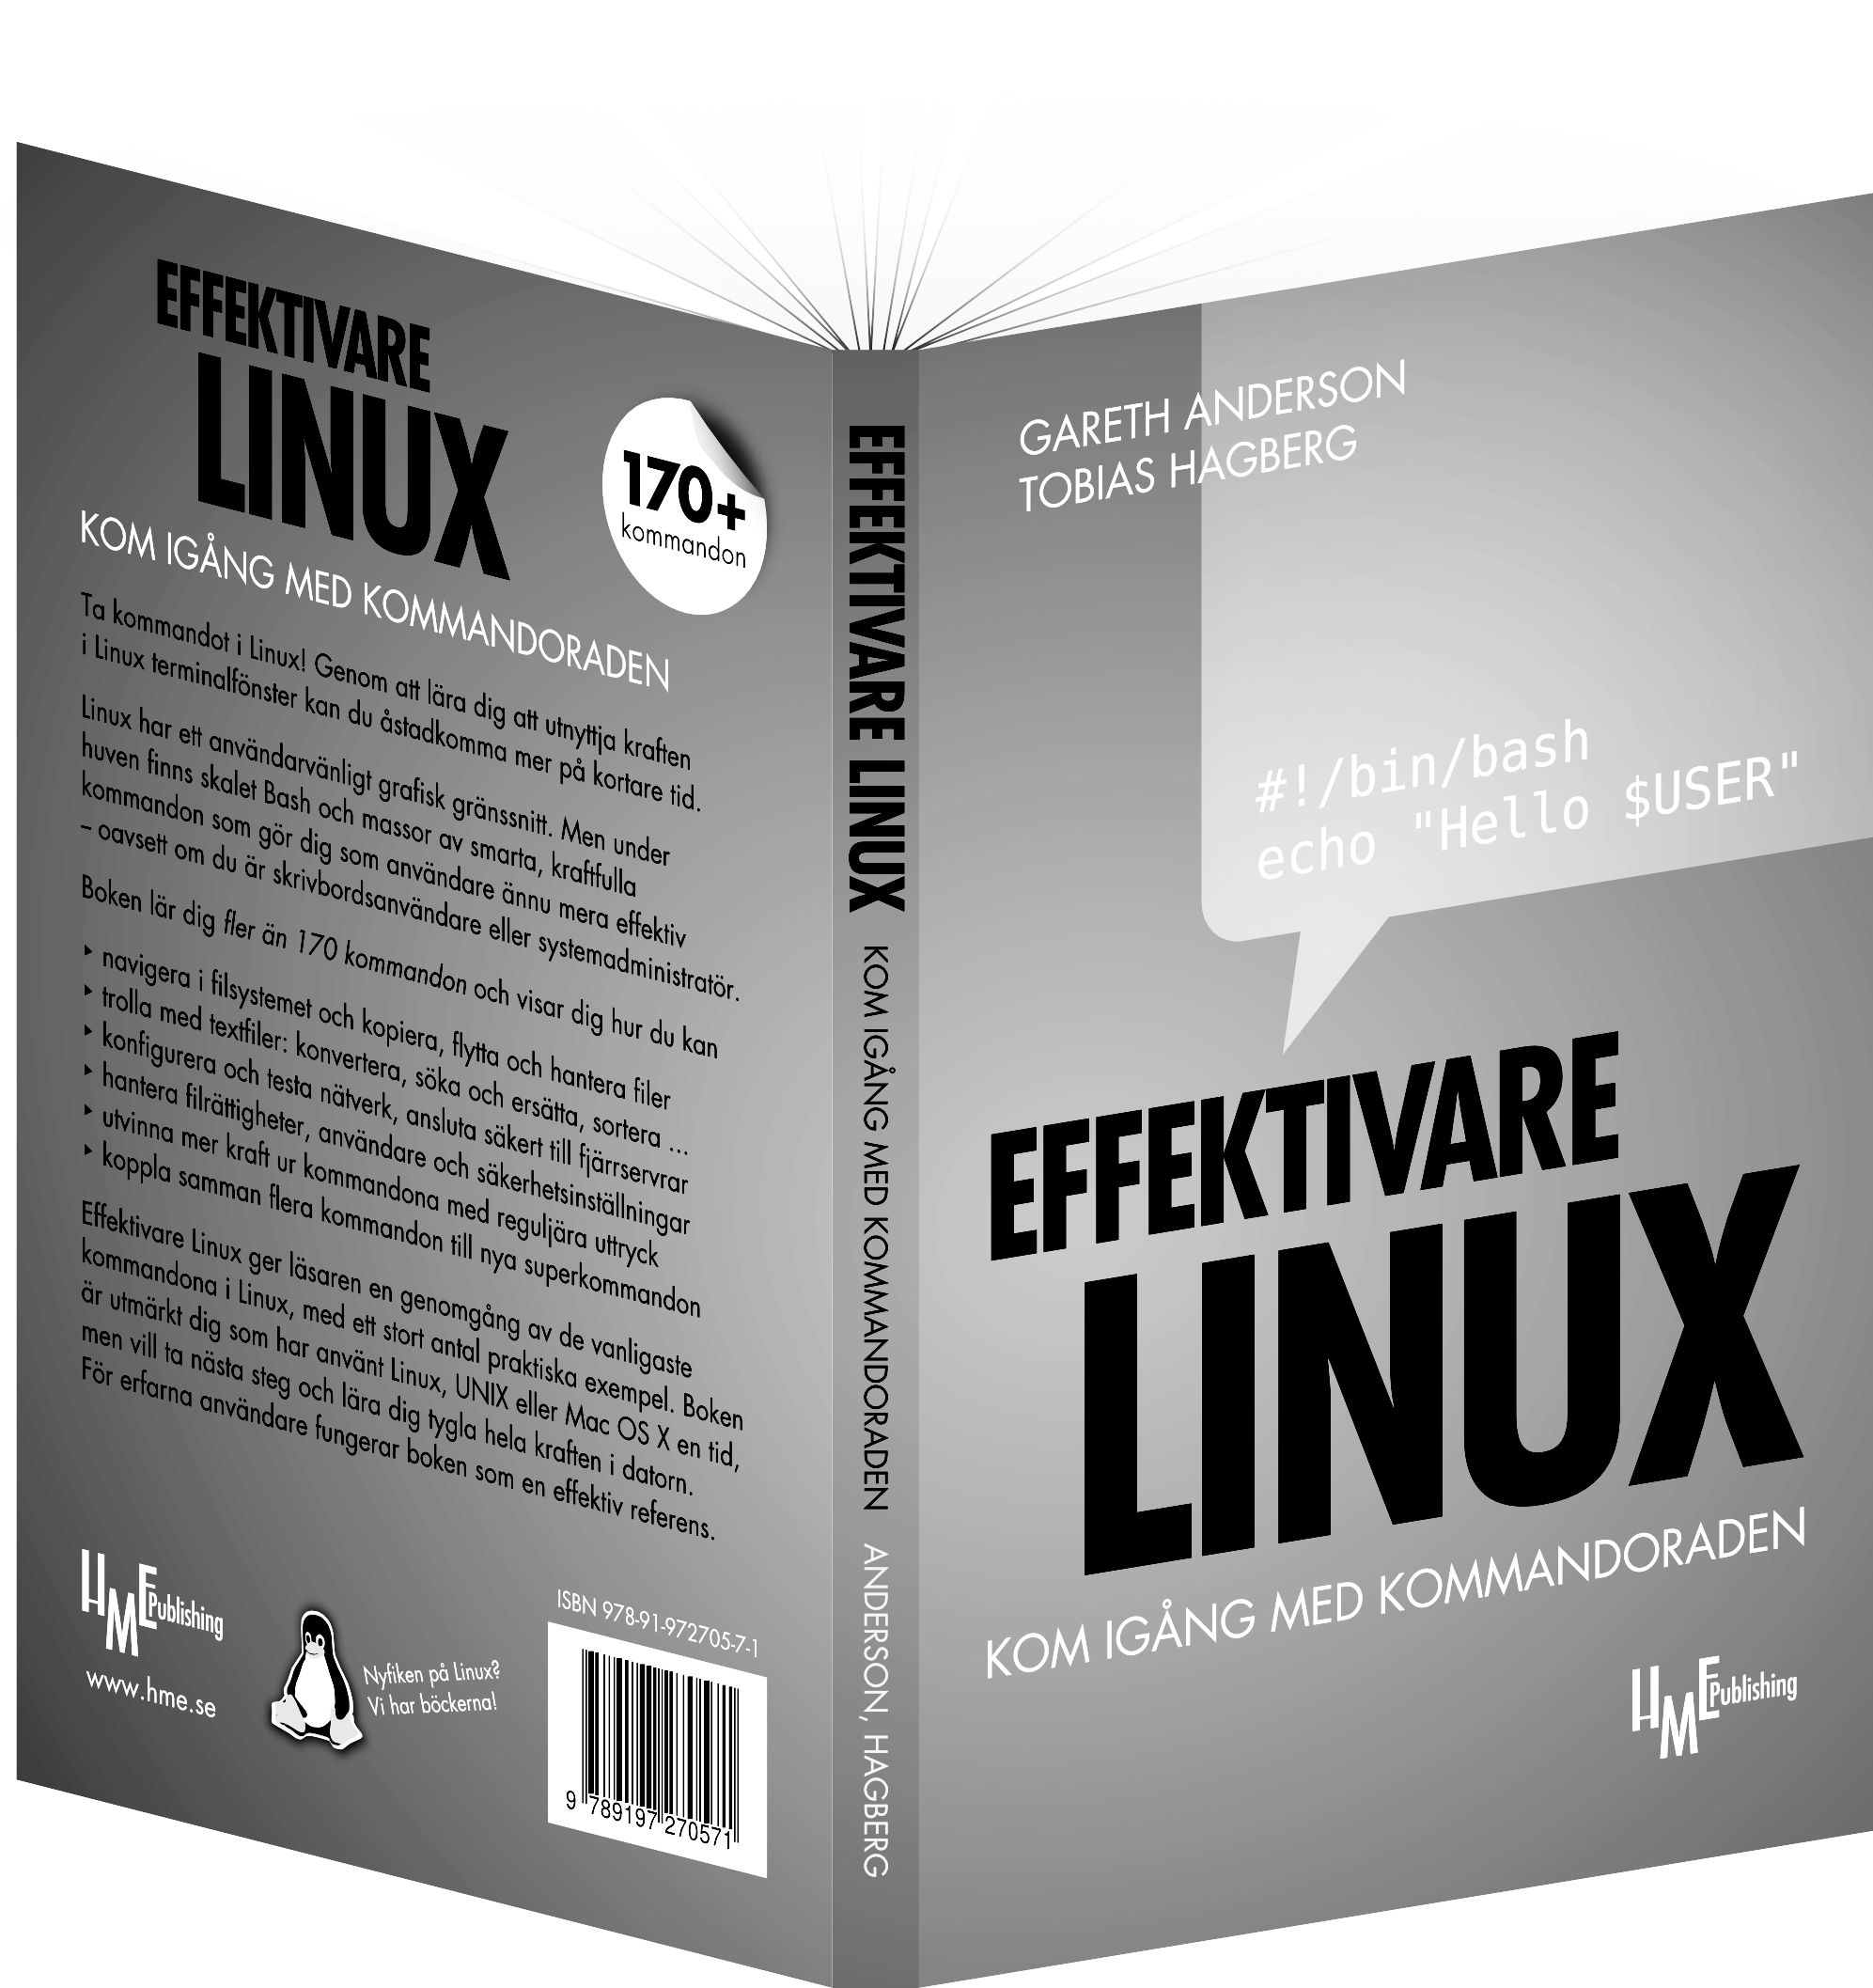
\includegraphics[width=56mm]{bilder804-all/el-reklam}

\end{center}

\medskip

\vspace*{0pt plus 1fill}

\noindent\textbf{\huge Ta kommandot i Linux!}

{\small

\begin{multicols}{2}

\bitem{\textbf{Effektivare Linux \\\noindent -- kom igång med kommandoraden}}
\bitem{av Gareth Anderson \\\noindent\& Tobias Hagberg}
\bitem{212 sidor, häftad}
\bitem{utkom i april 2008}
\bitem{ISBN 978-91-972705-7-1}

\medskip

Effektivare Linux -- kom igång med kommandoraden lär läsaren att utnyttja kraften i Linux terminalfönster för att åstadkomma mer på kortare tid.

\medskip

Linux har ett användarvänligt grafisk gränssnitt. Men under huven finns skalet Bash och massor av smarta, kraftfulla kommandon som gör dig som användare ännu mera effektiv -- oavsett om du är skrivbordsanvändare eller systemadministratör.

\medskip

Boken lär läsaren fler än 170 kommandon och visar pedagogiskt hur man kan 

\begin{itemize}
\pitem navigera i filsystemet och kopiera, flytta och hantera filer
\pitem trolla med textfiler: konvertera, söka och ersätta, sortera text
\pitem konfigurera och testa nätverk, ansluta säkert till fjärrservrar
\pitem hantera filrättigheter, användare och säkerhetsinställningar
\pitem utvinna mer kraft ur kommandona med reguljära uttryck
\pitem koppla samman flera kommandon till nya superkommandon
\end{itemize}

Effektivare Linux ger läsaren en genomgång av de vanligaste kommandona i Linux, med ett stort antal praktiska exempel. Boken är utmärkt för Linuxanvändare som vill ta nästa steg och lära sig tygla hela kraften i datorn. 
\end{multicols}

}

\vspace*{0pt plus 2fill}

{\Large

Läs mer på hme.se/katalog/2-2-44

}

\vspace*{0pt plus 6fill}

\hfill\noindent
\includegraphics[width=22mm]{bilder804-all/logo_final_bw}

\newpage

~

\end{document}

%%endskip

